\documentclass[a4paper,12pt,twoside]{book}
%\documentclass[a4paper,12pt,leqno]{book}
\usepackage{amsmath}
\usepackage{array}
\usepackage{latexsym}
\usepackage{amsfonts}
\usepackage{upgreek}
%\usepackage{cite}
\usepackage{color}
\usepackage{colortbl}
\usepackage[usenames,dvipsnames]{xcolor}
%\usepackage[top=2cm, bottom=2cm, left=1.5cm, right=1.5cm]{geometry}
\usepackage[titletoc]{appendix} 
%\usepackage{multirow}
\usepackage{pgf}
\pagestyle{myheadings} \markboth{SEAPODYM-MASS Reference Manual}{Release 4.0}

\newcommand\doublespacing{\baselineskip=1.6\normalbaselineskip}
%\usepackage[pdftex,final]{graphicx}
\usepackage{rotating}
\usepackage{textcomp}
\usepackage{lineno}
\usepackage{caption}
\usepackage{subcaption}

\renewcommand{\thesubfigure}{\alph{subfigure}}
\usepackage{longtable}
 
\renewcommand{\bibname}{References}
\usepackage[sectionbib]{natbib}

\usepackage[T1]{fontenc} % to make words with '_' searchable, but requires 'lmodern' to look pretty
\usepackage{lmodern} 

\usepackage{etoolbox}
%\usepackage{enumitem} to use with horisontal spacing, e.g. \begin{enumerate}[leftmargin=4cm]


\usepackage{multirow}
\let\cite=\citen
\newcommand\help[1]{{\color{red}(#1 ?)\normalcolor}}

%% Make URLs clickable
\usepackage[colorlinks, bookmarks=true, linkcolor=blue, urlcolor=blue,citecolor=black]{hyperref}

%% package to make URLs word wrap nicely
\usepackage{breakurl}
%% to have the choice of color 
\newcommand{\myhref}[3][black]{\href{#2}{\color{#1}{#3}}}

%\hyperref[sec:hello]{this section}

\usepackage{comment}
\usepackage{float}

%% Code highlighting
\usepackage{listings}

\usepackage[pass]{geometry}


%\patchcmd{\thebibliography}{\chapter*}{\section*}{}{}

\setlength{\oddsidemargin}{0pt}
\setlength{\evensidemargin}{\oddsidemargin}
\setlength{\textwidth}{6.5truein}
\newlength{\fullwidth}  \setlength{\fullwidth}{\textwidth}
\newlength{\fullheight} \setlength{\fullheight}{\textheight}
\newlength{\halfheight} \setlength{\halfheight}{0.375\fullheight}

\colorlet{config}{Orange}
\colorlet{forcing}{Green}
\colorlet{control}{Red}
\colorlet{cohort}{Blue}
\colorlet{species}{Turquoise}

%%% OT: macros

\newcommand{\config} {\textbf{\textcolor{config}{[config]}}}
%\newcommand{\model} {\textbf{\textcolor{model}{[model]}}}
\newcommand{\forcing}{\textbf{\textcolor{forcing}{[forcing]}}}
\newcommand{\control}{\textbf{\textcolor{control}{[control]}}}
\newcommand{\cohort}{\textbf{\textcolor{cohort}{[cohort]}}}
\newcommand{\species}{\textbf{\textcolor{species}{[species]}}}
\newcommand{\minitab}[2]{
  \renewcommand{\arraystretch}{0.6}
  \begin{tabular}{@{}l@{}}
    #1\\
    #2
  \end{tabular}
}
%%% / OT: macros

%Guillaume packages----------------------------------------------------
\usepackage{makecell} %%guillaume
\newcommand{\bracedincludegraphics}[2][]{%
  \sbox0{$\vcenter{\hbox{\includegraphics[width=0.4\textwidth]{#2}}}$}%
  \overbrace{\left.
    \vphantom{\copy0}{\box0}
  \kern-\nulldelimiterspace\right\rbrace}^{\textsc{\normalsize{NLON}}}}
%----------------------------------------------------------------------

\newcommand{\argmin}{\operatornamewithlimits{argmin}}	

%\title{A reference manual for\\ \vspace{0.5cm}  \LARGE{\bfseries{SEAPODYM-MASS version 4.0}}\\ \Large\slshape{Spatial Ecosystem and POpulation DYnamics Model} \\ \Large\slshape{for Migratory Age-Structured Stocks} \\}
%\author{I. Senina, O. Titaud, G. Briand, and P. Lehodey}
%
%\date{}
%
%\frenchspacing
%\maketitle

\begin{document}
\newgeometry{top=1cm,bottom=3cm,left=2cm,right=2cm}
\begin{titlepage}
\centering

\includegraphics[height=2cm]{intro/figs/SPC-CPS-logo_27_stars} \hspace{1.5cm}
\includegraphics[height=2cm]{intro/figs/logo-PFRP-large} \hspace{1.5cm}
\includegraphics[height=2cm]{intro/figs/logo-CLS}
\noindent{\color{gray}\rule{16cm}{0.4pt}}

\vspace{4cm}

{\fontsize{36pt}{42pt} \bfseries \color{teal} SEAPODYM \par}

\vspace{3.5cm}

%\noindent\rule{14cm}{0.4pt}

%{\Large\scshape{ A reference manual }\\}
{\Large \slshape \bfseries{Spatial Ecosystem and POpulation DYnamics Model} \\ \Large\slshape{for Migratory Age-Structured Stocks \par}}

\vspace{1.5cm}
{\large Inna Senina, Olivier Titaud, Guillaume Briand, and Patrick Lehodey \par}

\vspace{3cm}
{\Large \scshape --version 4.0-- \par}

\vspace{5cm}

\noindent{\color{gray}\rule{5cm}{0.4pt}}

{\large June 2022 \par}


\vfill

\end{titlepage}
\restoregeometry

%\clearpage
%%%%%%%%%%%%%%%%%%%%%%%%%%%%%%%%%%%%%%%%%%%%%%%%%%%%%%%%%%%%%%%%%%%%%%%%%%%%%%%%%%%%%%%%%%%%%%%%%%%
%\vspace{1.0cm}
\begin{comment}
\noindent Copyright \copyright  2022 by SPC\footnotemark[1], PFRP\footnotemark[2] and CLS\footnotemark[3].

\footnotetext[1]{Oceanic Fisheries Programme, Secretariat of the Pacific Community, BPA5 Noumea, New Caledonia}
\footnotetext[2]{Pelagic Fisheries Research Program, University of Hawaii at Manoa. 1000 Pope Road, Honolulu, HI 96822 United States}
\footnotetext[3]{Marine Ecosystems Modelling, CLS, Sustainable Fisheries Management Business Unit. 11 rue Hermes, 31520 Ramonville Saint-Agne, France}
\end{comment}
%\section*{LICENSE}

THE PROGRAM (AS DEFINED BELOW) IS PROVIDED UNDER THE TERMS OF THIS LICENSE. THE
PROGRAM IS PROTECTED BY COPYRIGHT AND/OR OTHER APPLICABLE LAW. ANY USE OF THE
PROGRAM OTHER THAN AS AUTHORIZED UNDER THIS LICENSE IS PROHIBITED.

BY EXERCISING ANY RIGHTS TO THE PROGRAM PROVIDED HERE, YOU ACCEPT AND AGREE TO
BE BOUND BY THE TERMS OF THIS LICENSE. THE LICENSOR GRANTS YOU THE RIGHTS
CONTAINED HERE IN CONSIDERATION OF YOUR ACCEPTANCE OF SUCH TERMS AND CONDITIONS.

1. Definitions

a. "Derivative Program" means a program based upon the Program or upon the
Program and other pre-existing programs in which the Program may be recast,
transformed, or adapted, except that a program that constitutes a Package will
not be considered a Derivative Program for the purpose of this License.

b. "Licensor" means the individual or entity that offers the Program under the
terms of this License.

c. "Original Author" means the individual or entity who created the Program.

d. "Package" means a software package, in which the Program in its entirety in
unmodified form, along with a number of other contributions, constituting
separate and independent programs in themselves, are assembled into a collective
package. Such a Package will not be considered a Derivative Program for the
purposes of this License.

e. "Program" means the copyrightable computer software, including executable and
source code, offered under the terms of this License.

f. "You" means an individual or entity exercising rights under this License who
has not previously violated the terms of this License with respect to the
Program, or who has received express permission from the Licensor to exercise
rights under this License despite a previous violation.

2. Fair Use Rights. Nothing in this license is intended to reduce, limit, or
restrict any rights arising from fair use, first sale or other limitations on
the exclusive rights of the copyright owner under copyright law or other
applicable laws.

3. License Grant. Subject to the terms and conditions of this License, Licensor
hereby grants You a worldwide, royalty-free, non-exclusive, perpetual (for the
duration of the applicable copyright) license to exercise the rights in the
Program as stated below:

a.    to reproduce the Program, to incorporate the Program into one or more
Packages, and to reproduce the Program as incorporated in the Packages;

b.    to distribute copies of the Program including as incorporated in Packages;

The above rights may be exercised in all media and formats whether now known or
hereafter devised. The above rights include the right to make such modifications
as are technically necessary to exercise the rights in other media and formats.
All rights not expressly granted by Licensor are hereby reserved.

4. Restrictions. The license granted in Section 3 above is expressly made
subject to and limited by the following restrictions:

a.    You may distribute the Program only under the terms of this License, and
You must include a copy of this License with every copy of the Program You
distribute. You may not offer or impose any terms on the Program that alter or
restrict the terms of this License or the recipients' exercise of the rights
granted hereunder. You may not sublicense the Program. You must keep intact all
notices that refer to this License and to the disclaimer of warranties. You may
not distribute the Program with any technological measures that control access
or use of the Program in a manner inconsistent with the terms of this License
Agreement. The above applies to the Program as incorporated in a Package, but
this does not require the Package apart from the Program itself to be made
subject to the terms of this License.

b.    You may not exercise any of the rights granted to You in Section 3 above
in any manner that is primarily intended for or directed toward commercial
advantage or private monetary compensation.

c.    If you distribute the Program or any Packages, You must keep intact all
copyright notices for the Program and give the Original Author credit reasonable
to the medium or means You are utilizing by conveying the name (or pseudonym if
applicable) of the Original Author if supplied; the title of the Program if
supplied. Such credit may be implemented in any reasonable manner; provided,
however, that in the case of a Package, at a minimum such credit will appear
where any other comparable authorship credit appears and in a manner at least
as prominent as such other comparable authorship credit.

5. Representations, Warranties and Disclaimer

a.    By offering the Program for public release under this License, Licensor
represents and warrants that, to the best of Licensor's knowledge after
reasonable inquiry:

i.      Licensor has secured all rights in the Program necessary to grant the
license rights hereunder and to permit the lawful exercise of the rights granted
hereunder without You having any obligation to pay any royalties, compulsory
license fees, residuals or any other payments;

ii.      The Program does not infringe the copyright, trademark, publicity
rights, common law rights or any other right of any third party or constitute
defamation, invasion of privacy or other tortious injury to any third party.

b.    EXCEPT AS EXPRESSLY STATED IN THIS LICENSE OR OTHERWISE AGREED IN WRITING
OR REQUIRED BY APPLICABLE LAW, THE PROGRAM IS LICENSED ON AN "AS IS" BASIS,
WITHOUT WARRANTIES OF ANY KIND, EITHER EXPRESS OR IMPLIED INCLUDING, WITHOUT
LIMITATION, ANY WARRANTIES REGARDING FITNESS OF THE WORK FOR A PARTICULAR
PURPOSE.

6. Limitation on Liability. EXCEPT TO THE EXTENT REQUIRED BY APPLICABLE LAW,
AND EXCEPT FOR DAMAGES ARISING FROM LIABILITY TO A THIRD PARTY RESULTING FROM
BREACH OF THE WARRANTIES IN SECTION 5, IN NO EVENT WILL LICENSOR BE LIABLE TO
YOU ON ANY LEGAL THEORY FOR ANY SPECIAL, INCIDENTAL, CONSEQUENTIAL, PUNITIVE OR
EXEMPLARY DAMAGES ARISING OUT OF THIS LICENSE OR THE USE OF THE PROGRAM, EVEN IF
LICENSOR HAS BEEN ADVISED OF THE POSSIBILITY OF SUCH DAMAGES.

7. Termination

a.    This License and the rights granted hereunder will terminate automatically
upon any breach by You of the terms of this License. Individuals or entities who
have received Packages from You under this License, however, will not have their
licenses terminated provided such individuals or entities remain in full
compliance with those licenses. Sections 1, 2, 5, 6, 7, and 8 will survive any
termination of this License.

b.    Subject to the above terms and conditions, the license granted here is
perpetual (for the duration of the applicable copyright in the Program).
Notwithstanding the above, Licensor reserves the right to release the Program
under different license terms or to stop distributing the Program at any time;
provided, however that any such election will not serve to withdraw this License
(or any other license that has been, or is required to be, granted under the
terms of this License), and this License will continue in full force and effect
unless terminated as stated above.

8. Miscellaneous

a.    Each time You distribute the Program or a Package, the Licensor offers to
the recipient a license to the Program on the same terms and conditions as the
license granted to You under this License.

b.    If any provision of this License is invalid or unenforceable under
applicable law, it shall not affect the validity or enforceability of the
remainder of the terms of this License, and without further action by the
parties to this agreement, such provision shall be reformed to the minimum
extent necessary to make such provision valid and enforceable.

c.    No term or provision of this License shall be deemed waived and no breach
consented to unless such waiver or consent shall be in writing and signed by the
party to be charged with such waiver or consent.

d.    This License constitutes the entire agreement between the parties with
respect to the Program licensed here. There are no understandings, agreements or
representations with respect to the Program not specified here. Licensor shall
not be bound by any additional provisions that may appear in any communication
from You. This License may not be modified without the mutual written agreement
of the Licensor and You.


\mbox{ }
\vspace{4cm}

\begin{center}{\copyright Pacific Community (SPC) 2022}\end{center}
All rights for commercial/for profit reproduction or translation, in any form, reserved. SPC authorises the partial reproduction or translation of this material for scientific, educational or research purposes, provided that SPC and the source document are properly acknowledged. Permission to reproduce the document and/or translate in whole, in any form, whether for commercial/for profit or non-profit purposes, must be requested in writing. Original SPC artwork may not be altered or separately published without permission.

\vspace{.5cm}

\begin{center} 
Original text: English

\vspace{2cm}
%Pacific Community Cataloguing-in-publication data

\vspace{7.5cm}
Prepared for publication at SPC’s headquarters. \\
B.P. D5, 98848 Noumea Cedex, New Caledonia, 2022 \\

www.spc.int | spc@spc.int

\end{center}

\chapter*{Preface}

SEAPODYM is a numerical modelling framework developed initially for investigating population dynamics of tunas under the influence of environment and fishing (\url{www.spc.int/ofp/seapodym}; \url{www.seapodym.eu}). The modelling effort started in 1995 at the Pacific Community (SPC) in Noumea, New Caledonia, under two consecutive EU-funded projects: SPR-TRAMP (1995-2000) and PROCFISH (2002-2005). The model development has continued under a grant from the Pelagic Fisheries Research Program (PFRP) at the University of Hawaii, allowing the implementation of a quantitative approach to estimate model parameters from massive spatio-temporal catch and size data (2004-2007). Since 2007 the development has been conducted at Collecte Localisation Satellites in Toulouse, France, in collaboration with the Oceanic Fisheries Program of SPC and under various research projects and funding provided by PFRP, the European Commission, Global Environment Facility (GEF) and the French National Research Agency. 

SEAPODYM includes two conceptually different dynamical models: i) a model of spatio-temporal dynamics of functional groups of zooplankton and micronekton, that is called SEAPODYM for Lower and Mid-Trophic Level (SEAPODYM-LMTL), and ii) a model describing full spatio-temporal dynamics of a single species population, called SEAPODYM for Migratory Age-Structured Stocks (SEAPODYM-MASS). The underlying continuous equations of SEAPODYM-MASS are classical advection-diffusion-reaction equations with an ageing term, describing the population dynamics in time, age and two-dimensional space. Using environmental data and outputs of the SEAPODYM-LMTL model as a forcing, this model predicts the biomass of modelled species as well as the catch and size frequency of catch based on parameter estimation and data assimilation techniques.

This reference manual describes version 4.0 of the SEAPODYM-MASS model and software, which has been updated and enhanced with a method for integrating tagging data to inform movement parameters, a new mechanism of modelling seasonal migrations between feeding and spawning grounds, revised definitions of habitat indices and movement rates, and a method to account for fishing mortality and to predict catch in the absence of fishing effort data. In addition to a complete model, this version allows running the simulations and estimations of movement parameters of a single or selected cohorts using tagging data and building the following minimal models with maximum likelihood estimation (MLE) method: i) a model of spawning habitat, ii) a model of feeding habitats for selected age classes, and iii) a model of virgin stock (without fisheries) with population density considered as an observation in the likelihood. These model applications can be used in model downscaling and/or adaptation to a different forcing dataset.

After a general introduction, this reference manual provides the full mathematical description of underlying continuous models, the numerical approximation scheme, a comprehensive guide on how to run numerical simulations and design various simulation studies, and a suite of numerical and statistical recipes for \textit{data assimilation} in complex spatio-temporal fisheries models, aimed at informing model parameters from massive geo-referenced data and providing quantitative model reconstruction of observed phenomena as well as unbiased model predictions of the independent observations.

\clearpage

\chapter*{List of changes from version 3.0}

\begin{itemize}
\item Integration of a movement model of tagged fish and tagging data likelihood.
\item Implementation of an alternative approach to account for fishing mortality and to
predict catch without fishing effort, i.e. based on observed catch only.
\item Introduction of an additional likelihood term to allow estimation of minimal biomass supporting observed catches.
\item A fully revised method to describe seasonal spawning migrations with a new mechanism of modelling large-scale migrations in the Eulerian model context.
\item Revised spawning habitat as a product of prey, predator and thermal functions, 
the latter with seasonal variable when playing the role of movement habitat of spawning adults.
\item Estimation of one additional parameter associated to each functional group of prey,
providing more flexibility in the representation of vertical behaviour and
access to preferred forage when computing the feeding habitat index.
\item Decoupled optimal temperature and thermal range for larval survival and for feeding habitat at age zero, to allow a separate estimation of these parameters.
\item Extension of sensitivity analysis by allowing two types of model global sensitivity runs: all-at-a-time (AAT) and one-at-a-time (OAT) runs, with names referring to the model parameter variations.
\item A standalone habitat models build {\bfseries seapodym\_habitats}, computing either spawning or multiple feeding habitats (at selected ages) in a simulation or optimisation mode, with associated parameter estimation from provided habitat fields.
\item A standalone model build {\bfseries seapodym\_densities} for population dynamics without fisheries, where biomass is considered both as observations and predictions in the likelihood.
\item A standalone model build {\bfseries seapodym\_fluxes} to compute the biomass flow rates between $n$ non-overlapping regions. The outputs of this application are stored in $n \times n$ matrices for each age class and quarterly time period.
\item Various code modifications to minimise the memory use during adjoint gradient computation.

\end{itemize}

\clearpage

{
  \hypersetup{linkcolor=black}
  \tableofcontents
}

\clearpage


\chapter*{Introduction}
\addcontentsline{toc}{chapter}{Introduction} 

\setcounter{figure}{0}
\renewcommand{\thefigure}{I.\arabic{figure}}

The Spatial Ecosystem And POpulation DYnamics Model (SEAPODYM) is being continuously enhanced to provide a general framework allowing integration of biological and ecological knowledge of migratory species, primarily tunas and potentially other oceanic top predator species, within a comprehensive description of the pelagic ecosystem. It includes detailed relationships between the population dynamics and basic biological and ecological functions, a realistic representation of the vertical oceanic habitat in terms of both physical and foraging conditions. The forage fields are predicted by a separate model in which various mid-trophic level organisms (micronekton) are classified by their diel migration pattern, and the spatiotemporal transfer of energy from oceanic primary productivity to the micronekton is described using an allometric scaling equation and passive transport of the biomass with oceanic water masses. The environmental variables that drive fish dynamics (temperature, currents, oxygen and primary production) are predicted by coupled physical--biogeochemical models. The model also includes a rigorous mathematical parameter estimation procedure using available catch and size frequency data. Because the model includes detailed representation of the biophysical environment of the species, the complete spatially explicit population dynamics can be described with a small number of parameters. In return, such a model depends strongly on the quality of environmental forcing variables. \\

When considering the definition of an ecosystem, that is, how assemblages of species are organised in space and time, and how they interact with each other and the physical environment, modelling the ocean pelagic ecosystem is obviously a challenge that requires drastic simplifications. These simplifications need to be considered carefully alongside the level of observations and knowledge that we have for each component of the system, to make sure that the model can be properly parametrised and can adequately describe observed processes. In addition, the model is focusing on the population dynamics and the fisheries of exploited species, as there is a special interest to provide a new generation of modelling tools for the management of these species, taking into account not only the impact of the fisheries but also the natural fluctuations of the populations in their climate-driven ecosystems. Top predators in the marine pelagic ecosystem are essentially opportunistic omnivorous predators. Their diets reflect both the faunal assemblage of the components of the ecosystem that they explore and their aptitude to capture prey species during different periods of the day (i.e., daytime, night-time and twilight hours). It seems that most of them are in the upper layer during the night. But high sensory specialisation (e.g., olfaction in sharks, vision in bigeye tuna, swordfish and cephalopods, and echolocation in marine mammals), and morphological and physiological adaptations (e.g., thermoregulation) allow them also to exploit the darker and colder, deeper layers. The three-layer ocean definition used for the mid-trophic (forage) species seems to match particularly well with the known vertical behaviour of large predators (Figure~\ref{Predators_3layers}). \\


\begin{figure}[H]  
	\centering
		\includegraphics[width=0.95\textwidth]{intro/figs/Fig_3layersPredators}
	\caption{Five typical vertical movement behaviours simulated using a three-layer and two-type-of-prey pelagic system (adapted from Dagorn et al. 2000): 1, epipelagic predators (e.g., skipjack tuna, marlins and sailfish); 2, predators moving between the surface and intermediate layers during the day (e.g., yellowfin tuna); 3, predators mainly in the intermediate layer during the day (e.g., albacore tuna); 4, predators moving between deep and intermediate layers during the day (e.g., blue shark); 5, predators mainly in the deep layer during the day (e.g., bigeye tuna and swordfish).}
	\label{Predators_3layers}
\end{figure}

Large pelagic predators are often exploited species for which there is detailed knowledge on biology, physiology, population structure and fisheries data. Describing the spatial dynamics of these fish populations at oceanic scales is of paramount importance for fisheries management, so as to understand and predict the consequences of fishing, climate change and changes in fishery management regulations. Many spatially explicit models have been developed for fish populations; however, most of them are Lagrangian models considering only passive movements of small fish or early life stage individuals transported by currents \citep*[see, e.g.,][]{DeAngelis, Rossi, Popova, Ramesh, vanSebille}. Parametrisation of Lagrangian models can only be done by manual calibration, using empirically derived parameter values or relying on estimates from external models \citep*[as in, e.g.,][]{Scutt}. Advection-diffusion-reaction (ADR) equations were suggested by many mathematical ecologists as an elegant solution to deal with complex spatio-temporal patterns arising from animal behaviour \citep*[see, e.g.,][]{Keller-Segel,Okubo80, Okubo-Levin, Murray, Grunbaum98, Grunbaum99, Flierl, Tyutyunov, TT, Berezovskaya,Petrovskii}. While ADR equations are unsuitable for low-abundance populations sparsely distributed in space, they provide a very convenient framework for modelling spatial dynamics of migratory species that occupy vast oceanic regions and may create low- and high-density concentrations. The movement dynamics within ADR equations are governed by the distribution of stimuli attracting or repulsing the population density. This classical approach has been thoroughly studied in theoretical movement ecology, widely used in various modelling applications and its interconnections with individual movements are well understood \citep{Okubo77, Okubo80, Grunbaum94, Grunbaum98, Grunbaum99,  Flierl, Turchin, Faugeras2007, Tyutyunov2013, TT}. 

The advantages of using ADR equations can be summarised as follows. While predicting the trajectory of a single individual is impossible due to the stochastic component of its movement, the evolution of density distributions of a large number of individuals can be effectively predicted in a continuous advection--diffusion framework \citep{Grunbaum99, Flierl, Tyutyunov}. In addition, explicitly modelling movement not only leads to a reduced number of model parameters and simplified local (in every position in space) functional responses \citep*[e.g.,][]{Arditi, TT}, but also allows considering simple aggregated statistics (e.g., mean squared step length) in model parametrisations \citep{Grunbaum98}. Moreover, incorporating biological-physical interactions by accounting for the impact of temporal and spatial environmental variability on population dynamics and thus reducing the number of model parameters is more straightforward in ADR equations \citep*[e.g.,][]{Grunbaum98, Flierl} than in classical, spatially aggregated stock assessment models operating in large management regions \citep{Punt}. In exchange for their parsimony, spatially explicit dynamic models applied to full-life-cycle fish population dynamics have higher dimensionality. The latter represents the cost for being more realistic models.\\

Being continuous, ADR equations allow implementation of quantitative methods to estimate model parameters from available observations \citep{Sibert, Senina08}. Nevertheless, before applying these models to solve fishery management problems, we need to be confident in the reliability of model predictions. Hence, we need to work on developing the dynamic model, providing adequate descriptions of observed phenomena, and improving the model structure, allowing quantitative dynamics, under the tight coupling of the model predictions to observations. \\

The SEAPODYM modelling approach for top predator population dynamics has greatly benefited from the work undertaken by \citet{Sibert} on implementation of continuous ADR equations to describe movement dynamics and estimate movement and mortality rates of tagged skipjack and yellowfin tunas \citep*[see also][]{Sibert-Fournier}. SEAPODYM has been continuously evolving since the initial development of a single-cohort tuna population model presented in \citet{Bertignac}. A few years later \citet{Lehodey2001} proposed a coupled predator--prey model with the model for tuna forage. In the study of \citet{Lehodey2003}, discrete-type age structured equations were added to the numerical solver of continuous ADR equations. The first fully parametrised and fully operational SEAPODYM model was presented in \citet{Lehodey2008}, and with an added parameter estimation method in \citet{Senina08}. The general scheme of the model and parameter estimation approach is shown in Figure~\ref{model_scheme}. \\

\begin{figure}[htbp]
	\centering
	\includegraphics[width=0.85\textwidth]{intro/figs/fig-scheme-old}
	\caption{General scheme of the model with optimization approach \citep[from][]{Senina08}.} 
	\label{model_scheme}
\end{figure}

The current model version is based on a continuous ADR equation with an ageing term, and is fully described in \citet{Senina20a,Senina20b}. The SEAPODYM modelling framework now includes several models, and allows, besides the full population dynamics model, computing and estimating the parameters of spawning and feeding habitats, modelling movement dynamics of tagged cohorts, and integrating tagging data to inform movement rates of modelled fish at different ages/sizes. The model can be now be parametrised through integration of industrial fisheries data and conventional as well as archival tagging data, and optimization is carried out using the maximum likelihood estimation approach. The implementation of adjoint code allows an exact, analytical evaluation of the likelihood gradient to be obtained. The approach to select the ``best parameter estimate'' is based on a series of computer experiments in order to i) determine model sensitivity with respect to variable parameters and, hence, investigate their observability; ii) estimate observable parameters and their errors; iii) justify the reliability of found solutions; iv) validate the parametrisation with independent information; and v) compute the errors of parameter estimates. \\

The continuous improvements in the model structure, the implementation of the numerical model coupled with the quantitative methods of parameter estimation allowed numerous model applications to different pelagic species such as Pacific skipjack tuna \citep{Lehodey2013,Senina20b}, Pacific yellowfin tuna \citep{Senina2015}, Pacific bigeye tuna \citep{Senina2021}, Atlantic albacore tuna \citep{Dragon2015,Senina20a}, South Pacific albacore tuna \citep{Lehodey2015,Senina20a}, Chilean jack mackerel \citep{Dragon2017} and Pacific swordfish \citep{Abecassis}. Informing model parameters through integration of various types of data for different migratory species thus showed that such models have the capacity to provide valid quantitative predictions of the species population dynamics, and can be used in the development of management strategies \citep{Sibert2012} and in investigating the climate change impacts \citep{Lehodey2010,Lehodey2013,Lehodey2015,Bell}. All examples of applications and related projects can be found in the dedicated websites (\url{www.seapodym.eu}; \url{www.spc.int/ofp/seapodym}).\\

This reference manual for the SEAPODYM-MASS model is constructed as follows. {\hypersetup{linkcolor=black} Chapter 1, {\bfseries ``\nameref{ch:model}}"} is devoted to the mathematical model and the dynamic processes it describes. It also details the underlying biological mechanisms behind the definitions of spawning and feeding habitats. {\hypersetup{linkcolor=black} Chapter 2, {\bfseries ``\nameref{ch:numerics}}"} describes the discretisation of model dimensions, the numerical model that is the approximation of the continuous ADR equations with an ageing term, its integration with alternating-direction implicit (ADI) method and the general algorithm implementation within the main time and age loop. {\hypersetup{linkcolor=black} Chapter 3, {\bfseries ``\nameref{ch:configurations}}"} provides detailed documentation on how to run the model simulation with predefined configurations. The input and output data files are also described in this chapter. {\hypersetup{linkcolor=black} Chapter 4, {\bfseries ``\nameref{ch:parametrisation}}"} reviews the methods to build up quantitative models. This final chapter is intended for advanced use of the model, providing the methods for the model application to the new species.

\setcounter{figure}{0}
\renewcommand{\thefigure}{\arabic{chapter}.\arabic{figure}}

\addcontentsline{toc}{section}{References}


\begin{thebibliography}{}

\bibitem[Lehodey et al., 1998]{Lehodey1998} Lehodey P., André J-M., Bertignac M., Hampton J., Stoens A. 1998. Predicting skipjack tuna forage distributions in the Equatorial Pacific using a coupled dynamical bio-geochemical model. \textit {Fisheries Oceanography} 7: 317–325.

\bibitem[Lehodey et al., 2010]{Lehodey2010} Lehodey, P.,  Murtugudde R., Senina I. 2010. Bridging the gap from ocean models to population dynamics of large marine predators: A model of mid-trophic functional groups. \textit{Progress in Oceanography}, Volume 84:69-84.

\bibitem[Lehodey et al., 2015]{Lehodey2015} Lehodey P., Conchon A., Senina I., Domokos R., Calmettes B. et al. 2015. Optimization of a micronekton model with acoustic data. ICES Journal of Marine Research. 53, 571-607. Science 72(5):1399–1412. \url{https:/doi.org/10.1093/icesjms/fsu233}

\end{thebibliography}


%%%%%%%%%%%%%%%%%%%%%%%%%%%%%%%%%%%%%%%%%%%%%%%%%%%%%%%%%%%%%%%%%%%%%%%%%%%%%%%%%%%%%%%%%%%%%%%%%%%

%%% Local Variables:
%%% TeX-master: "../Seapodym_user_manual.tex"
%%% End:
\chapter{The fish population dynamics model}
\label{ch:model}

\section{Underlying equations}
\label{sec:underlying-equations}

The general model of SEAPODYM is based on a classical advection--diffusion--reaction (ADR) equation. Let $N(a,t,\mathbf{x})$ be the density of the fish population at age $a \in \left[0,\bar{a}\right]$, at time $t \in \left[t_0,t_{\text{fin}}\right]$ and at position $\mathbf{x}=(x,y) \in \Omega \in \mathbf{R}^2$. Herein for brevity we omit notations of age, time and space, and use the gradient operator $\nabla = (\partial_x, \partial_y)^{\text{T}}$ and the divergence operator of a two-dimensional vector field $\text{div}(\mathbf v)=\partial_x u+\partial_y v$.
\begin{linenomath}
The continuous version of SEAPODYM describing spatial, temporal and age dynamics of fish population density $N$ is represented by the system of ADR equations with an ageing term, the initial and boundary conditions:
\begin{align}
& \partial_t N+\partial_a N =-\text{div} (\mathbf{v} N ) +\nabla (D \nabla N) - M N \label{eq:model-1}\\
& N(a,\mathbf{x},t_0)  = N_0 (a,\mathbf{x})  \label{eq:model-2} \\
& N(0,\mathbf{x},t) =  S(t,\mathbf{x}) \label{eq:model-3}\\
& \mathbf n \cdot \mathbf v \Bigr\rvert_{\mathbf x \in \partial \Omega} = \mathbf n \cdot\nabla N \Bigr\rvert_{\mathbf x \in \partial \Omega} = 0 \label{eq:model-4}  
\end{align}
\end{linenomath}
where 
\begin{itemize}

\item[] $\mathbf{v}={\mathbf{v}}_c+{\mathbf{v}}_N$ is the velocity field including velocity of ocean currents ${\mathbf{v}}_c$ and directed movement velocities of population density ${\mathbf{v}}_N$ (see eqs.~\ref{eq:mean-currents} and \ref{eq:active-movement-velocity});
\item[] $D$ is the diffusivity (see eq.~\ref{eq:diffusion}); 
\item[] $M = m_N + m_F$ is the total mortality that is the sum of natural $m_N$ and fishing $m_F$ mortality rates (see eqs.~\ref{eq:Mvar} and \ref{eq:FM}); 
\item[] $N_0(a,\mathbf{x})$ in (eq.~\ref{eq:model-2}) is the initial value of the state vector, i.e. the population density for all ages $a \in \left[0,\bar{a}\right]$ in the two-dimensional space, where $\bar{a}$ is the maximal age of individuals in a given population; 
\item[] $S(t,\mathbf{x})$ in (eq.~\ref{eq:model-3}) gives the new recruited biomass after spawning, i.e. the boundary condition at $a=0$ (see eqs.~\ref{eq:larvae} and \hyperref[sec:reproduction]{\ref*{sec:reproduction}}); 
\item[] Neumann zero-flux boundary conditions (eq.~\ref{eq:model-4}) imply impenetrability of the two-dimensional domain $\Omega\in\mathbb{R}^2$ boundaries, $\partial \Omega$; 
and
\item[] $\mathbf{n}$ is the unit normal vector to $\partial\Omega$.
\end{itemize}


In addition to age dynamics, the model (\ref{eq:model-1}--\ref{eq:model-3}) describes the dynamics of four life stages. These are larvae, small juveniles, immature (young) and mature (adult) fish (Table \ref{tab:life_stages}). The reasoning behind considering these life stages is their different movement dynamics. Larvae drift in the surface where they are passively transported by ocean currents; hence their survival depends on the local environmental conditions in the sites to which they are transported. Small juveniles (for tunas, up to 3 months of age, for other fish species, age classes which cannot be considered autonomous in terms of movements) occupy the epipelagic layer, through which they start performing diel migrations to avoid predation. However, their large-scale horizontal movements are still passive and depend on currents in this layer. In the next life stage of young immature fish, in addition to being passively transported by ocean currents, fish can undertake directed movements in search of food. At the fourth life stage, mature adults, the fish have two drivers of movement -- survival, that is, searching for food, and reproduction, that is, moving to habitats that provide optimal conditions for spawning and for survival of larvae. Note that dynamics of all life stages are modelled by the general model (eqs.~\ref{eq:model-1}--\ref{eq:model-3}); however, the rates of reproduction, mortality and movement are considered differently. 


\begin{table}[!htb]
  \caption{
    Considered life stages of a modelled population. The column ``driver'' specifies the biological driver for active movement (both directed and non-directional).
  }
\centering
  \begin{tabular}{p{2.75cm}|p{2.25cm}|p{1.75cm}|p{3.5cm}|p{4cm}}
  \hline
%  \begin{tabular}{p{2.75cm}p{2.75cm}p{1.75cm}p{3.75cm}p{3cm}}
    \textbf{Life stage} & \textbf{Ages, $a$} & \textbf{Layer} & \textbf{movement} &\textbf{Driver}\\
    \hline   \hline
    Larvae         & $a=0$ & surface & passive drift & none\\
%    \hline
    Small juveniles& $0 < a \leq a_J$ & epipelagic & passive drift & none\\     
%    \hline
    Young adults   & $a_J <  a \leq a_Y$ & all & passive and active & survival \\   
%    \hline
    Mature adults  & $a_Y < a \leq \bar{a}$ & all & passive and active & survival, reproduction\\
    \hline%\hline
  \end{tabular}
\label{tab:life_stages}   
\end{table}

\section{Dynamic processes}
\label{sec:model-dyn}

SEAPODYM follows a biophysical approach explicitly describing the spatio-temporal dynamics of a species population density arising from animal behaviour as a response to environment. The environment is described by physical, biogeochemical and biological variables derived from external models. These variables are temperature, currents, dissolved oxygen, primary production, euphotic depth and density of micronektonic organisms that are the prey of tunas and other large predators (see section~\ref{sec:model-forcing}). As seen from the model (eqs.~\ref{eq:model-1}--\ref{eq:model-3}), the fish population dynamics in SEAPODYM are resolved in four dimensions: two-dimensional space, time and age. The vertical dimension is simplified into three pelagic layers. 

Two main drivers of animal behaviour, reproduction and survival, are considered. To integrate them into the model, two types of habitat indices, spawning $H_s$ and feeding $H_a$, are defined. Definitions of species habitats are based on empirical evidence. A thermal habitat of tuna species is derived from an individual heat budget model. The feeding habitat is computed according to the accessibility of tuna predator cohorts to the different vertically migrating and non-migrating micronekton (mid-trophic) functional groups. The spawning habitat is based on temperature and density of predators and food for larvae in the spawning sites. These habitats, as well as the movements, reproduction and survival, are driven by a biophysical environment predicted from a coupled ocean physical--biogeochemical model. 


\subsection{Species environment}\label{sec:model-forcing}

The species environment is described by the spatio-temporal fields of the following variables: i) physical -- temperature and ocean currents, ii) biochemical -- dissolved oxygen concentration, primary production and euphotic depth, and iii) biological -- the food resource for the species (see Table~\ref{forcing}). The temperature, dissolved oxygen concentration, and zonal/meridional currents are the three-dimensional outputs of coupled ocean general circulation (OGCM) and biogeochemical (BGCH) models. The euphotic depth and integrated primary production are the two-dimensional outputs of either BGCH models or observation-based empirical models. Three pelagic layers represent a simplified vertical dimension of SEAPODYM: the surface epipelagic layer, the subsurface mesopelagic layer and the deep mesopelagic layer. The current definition of these layers is based on the euphotic depth and originates from the definition of six functional groups of micronekton (Figure~\ref{fig:mnk_groups}). 


\begin{table}
\caption{Forcing variables used in SEAPODYM applications. The column {\bfseries Model} refers to the external model type. }
%\vspace{0.5cm}
\begin{tabular}{>{\bfseries}m{1.5cm}m{2.25cm}m{11.5cm}}
\hline
{Model} & {\textbf{Variables}} & {\textbf{ Description}}\\
\hline
\hline
\multicolumn{3}{c}{\cellcolor[gray]{0.8}\textit{Physical forcing}}\\
\footnotesize{OGCM} & $T$, $u,v$ &  Ocean reanalysis by general circulation model with atmospheric forcing based on meteorological observations. \\

\multicolumn{3}{c}{\cellcolor[gray]{0.8}\textit{Biogeochemical forcing}}\\

\footnotesize{BGCH} & $P$, $O_2$, $z_e$ & Primary production, dissolved oxygen and euphotic depth, either  predicted by BGCH model coupled to OGCM, or by empirical model (e.g. VGPM) derived from satellite data. \\


\multicolumn{3}{c}{\cellcolor[gray]{0.8}\textit{Biological forcing}}\\
\footnotesize{LMTL} & $F$, $Z$ & Six micronekton groups and one lower-trophic level group (zooplankton) predicted by SEAPODYM-LMTL model with the above forcing, excluding dissolved oxygen. \\
\hline
\label{forcing}
\end{tabular}
\end{table}

First, all three-dimensional environmental variables are averaged over three pelagic layers (Figure~\ref{fig:forcing_integration}). These integrated variables are then used to force the SEAPODYM-LMTL (Lower and Mid-Trophic Level) model. The SEAPODYM-LMTL model relies on primary production, temperature and ocean currents to simulate the biomass of six functional groups of micronekton, that is, mid-trophic-level prey organisms of tunas, residing or migrating through three pelagic layers within the upper 1000~m of the water column. The depth $\mathbf{z}$ of pelagic layers is linked to the depth of euphotic layer $z_e$ as follows: 
\begin{equation}\label{eq:pelagic-layers}
\mathbf{z}=(1.5 z_e,4.5 z_e,min(10 z_e,1000)). 
\end{equation}

\begin{figure}[H]
\centering
 \includegraphics[width=0.92\textwidth]{chapter1/figs/mnk-groups}
 \caption{The definition of micronekton functional groups by their vertical diel behaviour. }
 \label{fig:mnk_groups}
\end{figure}

\begin{figure}
 \centering
 \includegraphics[width=0.3\textwidth]{chapter1/figs/T-3d-grid}
 \includegraphics[width=0.3\textwidth]{chapter1/figs/T-3d-grid-zeu}
 \includegraphics[width=0.32\textwidth]{chapter1/figs/T-2d-grid}
 \caption{The integration of three-dimensional environmental variables. Here three-dimensional temperature (left) is integrated over three pelagic layers (middle) and divided by each layer's thickness to provide the two-dimensional mean fields of each forcing variable.}
 \label{fig:forcing_integration}
\end{figure}

The definition \eqref{eq:pelagic-layers} of pelagic layers in SEAPODYM is derived from the diurnal patterns in vertical distributions of micronektonic species shown by acoustic observations (see \citet{Lehodey2015} for further details on vertical layer definition and the SEAPODYM-LMTL model). The spatio-temporal fields of modelled micronekton together with the physical and biochemical variables are used to describe the preferred habitats of the large pelagics for foraging and spawning and to predict their temporal and spatial dynamics. 


Let us denote $var_{\mathbf{z}}(t,\mathbf{x})$, the forcing variable averaged over vertical layer $\mathbf{z}$, where $var$ can be either water temperature $T$, dissolved oxygen $O_2$, or ocean currents $u$ and $v$. As mentioned above, the primary production $P =P(t,\mathbf{x})$ is integrated through the whole water column (knowing that most of it is concentrated in the euphotic layer). Vertically integrated primary production is given in units of $\text{mmol C} \text{ m}^{-2} \text{d}^{-1}$. The density of micronekton $F_{z_d z_n}=F(t,\mathbf{x},z_{d},z_{n})$ refers to the modelled density of small nektonic organisms (representing prey of modelled predatory species) aggregated into a functional group by their vertical behaviour, that is, all inhabiting layer $z_d$ and $z_n$ during the day and night respectively, as shown in Figure~\ref{fig:mnk_groups}. For brevity, hereafter we omit dimensional notations (time, 2D space) for SEAPODYM forcing variables once they are defined. Also, for convenience let us represent all prey functional groups as a diagonal matrix of dimension $dim(\mathbf z) \times dim(\mathbf z)$,

\begin{equation}
 \mathbf{F} = \left( 
  \begin{array}{ccc}
	F_{11} & 0 & 0 \\
	F_{21} & F_{22} & 0 \\
	F_{31} & F_{32} & F_{33}
  \end{array} \right)
\label{eq:F}
\end{equation}

\noindent where the rows and columns show the composition of vertical layers during the day and night respectively.  

\subsection{Spawning habitat}\label{sec:spawning-habitat}
The spawning habitat describes the ensemble of environmental conditions that are favourable for spawning and optimal for larvae survival. In other words, the spawning habitat describes the ensemble of conditions that constrain larval production and mortality, and affect the subsequent recruitment. This habitat then represents the following four mechanisms:
\begin{itemize}
	\item changes in the spatial extent of the spawning habitat with temperature;
	\item coincidence of spawning with presence or absence of food for larvae (micro-zooplankton, approximated by primary production), that is, the match/mismatch mechanism proposed by Cushing (1975);
	\item coincidence of spawning with presence or absence of predators of larvae (that are the micronektonic organisms, i.e., the prey of adults); and
	\item redistribution of larvae by the oceanic circulation, which can retain larvae in favourable areas with lower natural mortality, or conversely move the larvae to unfavourable zones where the natural mortality will be higher. 
\end{itemize}

The favourability of tuna habitat in terms of spawning success and larvae survival depends on three oceanic variables -- sea surface temperature ($SST(t,\mathbf{x})$), prey of larvae ($\Lambda(t,\mathbf{x})$, can be either plankton density or primary production as a proxy), and density of predators of larvae present in the surface layer, which are also the food for spawners ($F_1(t,\mathbf{x})$, surface micronekton, see below).  

The index of spawning habitat, $H_s(t,\mathbf{x}) \in (0,1)$, is defined as the following product (for brevity, we omit here the dimensional notations of environmental variables, micronekton density and habitats):

\begin{align}
	H_s = f_1(SST;{T}^{*},\sigma) \times f_2(\Lambda,\alpha) \times f_3(F_1,\alpha_F,\beta_F),
\label{eq:spawning_habitat}
\end{align}

\noindent requiring that all three environmental conditions are optimal for the species for the habitat index to be maximal. These three functions (see Figure~\ref{fig:reproduction-funcs}) are defined between 0 and 1 as follows. The thermal conditions are described by

\begin{equation}
f_1 = e^{-\frac{\left(SST-T^*\right)^2}{2\sigma^2}},
\label{eq:spawning-thermal}
\end{equation}

\noindent a Gaussian function with two parameters, ${T}^{*}$ and $\sigma$, being the optimal temperature and thermal tolerance interval of larvae respectively. The function $f_2$ is the analogue of the Holling type III functional response function with $n=2$:

\begin{equation}
f_2=\frac{\Lambda^n}{\alpha+h\Lambda^n},
\label{eq:spawning-prey}
\end{equation}

\noindent where handling time $h=1$ (to allow the function scaling within $[0,1)$ interval) and $\alpha\ge0$ the inverse of searching efficiency defining the shape of functional response to the prey densities (no response with $\alpha=0$, mostly hyperbolic within the effective range of prey densities as the inflection point $\Lambda=\sqrt{\frac{\alpha}{3}}$ gets too close to 0 with small $\alpha$ and marked logistic relationship with large enough $\alpha$). Note that when using primary production $P$ as a proxy for the density of phyto- and zooplankton, which are the actual prey of larvae, we should convert primary production to the wet weight of plankton. So if ocean primary production $P$ is given in mmol$\cdot$C$\cdot$m$^{-2}$, we use the energy transfer constant $E=0.354$ to compute the part of $P$ that will be transferred to lower-trophic level groups \citep*[see][]{Lehodey2015} and the conversion factor $c=0.1415$~gWW$\cdot$mmol$^{-1}$~C \citep{Iverson}, so that $\Lambda=cEPt$, the $t$ being the unit time of production $P$, provides the wet weight of plankton species in the units of g$\cdot$m$^{-2}$. 


The third function, $f_3$, is the log-normal distribution function rescaled on $(0,1)$ allowing selection of the optimal window of micronekton densities $F_1$ in the surface layer:

\begin{equation}
f_3 = \frac{1}{F_1 e^{0.5\beta^2_F-\alpha_F}} e^{-\frac{\left(\log{F_1}-{\alpha_F}\right)^2}{2\beta^2_F}}
\label{eq:spawning-pred}
\end{equation}

\noindent where parameters $\alpha_F$ and $\beta_F$ are the mean and standard deviation of log-normal distribution function, and the surface micronekton densities $F_1$ (1 is the layer index) is computed as follows: 

\begin{equation}
F_1 = \tau {\mathbf F_{1 \cdot}}{\mathbf \delta} +(1-\tau) {\mathbf {F_{\cdot 1}}^{\mathsf{T}}} {\mathbf \delta}
\label{eq:pred-surface}
\end{equation}

\noindent with $\mathbf{\delta}=(1,1,1)^{\mathsf{T}}$ and $\tau$ is the proportion of light hours in a 24-hour cycle. In other words, $F_1$ is the density of all micronektonic organisms present in the epipelagic layer during the day, ${\mathbf F_{1 \cdot}}$, and during the night, ${\mathbf {F_{\cdot 1}}^{\mathsf{T}}}$, either residing or migrating here from deeper layers. However, larvae predation is likely maximal during daytime and twilight periods, and therefore only two twilight hours are considered in the second term; hence the formula~\ref{eq:pred-surface} simplifies to 

\begin{equation}
F_1 = \tau {\mathbf F_{1 \cdot}}{\mathbf \delta} + {\mathbf {F_{\cdot 1}}^{\mathsf{T}}} {\mathbf \delta}/12
\label{eq:pred-surface2}
\end{equation}

%the density of predators of larvae ~\ref{eq:pred-surface} is computed as the sum of mid-trophic biomass in the epipelagic layer during daytime (the daylength) and epi- and migrants from deeper pelagic mid-trophic biomass during the sunrise and sunset hours only. In practice, in model applications

\subsection{Reproduction}\label{sec:reproduction}
Successful larval recruitment is linked to both the spawning stock density and the conditions of larvae survival. Hence, the number of recruited larvae $N(0,t,\mathbf{x})$ is the product of $H_s$ (eq.~\ref{eq:spawning_habitat})  and the stock-recruitment function of density of mature adults.

The total amount of  mature adults in each position of two-dimensional space, $\hat{N}(t,\mathbf{x})$, is computed using the continuous maturity function $\mu=\mu(a)$ obtained from external studies (see section~\ref{sec:sp-biology}) and the density of adult tuna predicted by the model (for brevity, hereafter we leave notation of age dimension and deliberately omit (time, 2D space) notations for SEAPODYM state variables):
\begin{equation}
	\hat{N} = \int_{a_J}^{\bar{a}}{\mu(a)N(a)da}
\label{eq:Nmature}
\end{equation}

\noindent where $a_J$ is the last age in a small juvenile stage and $\bar{a}$ is the maximal age of individuals in the population. The number of new recruits at zero age, $N(0,t,\mathbf{x})$, that is, the term $S$ in eq.~\ref{eq:model-1}, is then the product of the Beverton--Holt stock-recruitment function \citep{Beverton-Holt} and the spawning habitat index:

\begin{equation}
	N(0) = H_s \frac{r\hat{N}}{1+b\hat{N}}
\label{eq:larvae}	
\end{equation}	

\noindent where $r$ is the reproduction rate and $b$ is a parameter defining the strength of the stock--recruitment relationship between the density of spawners, $\hat{N}$ (in $\text{Nb}\cdot\text{km}^{-2}$, Nb - number of individuals), and those of larvae, $N(0)$, survived and recruited to the first age class (Figure~\ref{fig:reproduction-funcs}). This relationship is suitable for opportunistic spawners, for which the spawning success depends on the local spawning habitat index and the adult biomass.   

\begin{figure}
 \centering
 \includegraphics[width=0.92\textwidth]{chapter1/figs/reproduction-funcs}
 \caption{Functions used in the definition of spawning habitat and reproduction: (a) Beverton--Holt stock--recruitment function, (b)thermal function $f_1$, (c) prey function $f_2$, and (d) predator function $f_3$, based on parameters estimated for bigeye tuna \citep{Senina2020b}.}
 \label{fig:reproduction-funcs}
\end{figure}

\subsection{Growth and maturity}\label{sec:sp-biology}

SEAPODYM uses the species' biological parameters estimated in external studies, which are usually obtained from fitting the classical \citet{Bertalanffy} growth equation either to data derived either from conventional tagging or from otolith increments. This equation assumes that as the organism ages, its length increases to an asymptote $\ell_{\infty}$, which is the greatest possible length that the organism can attain under the given conditions:

\begin{equation}
\ell(a) = \ell_{\infty}\left(1- \mathrm{e}^{(-k(a-a_0)}\right)
\label{eq:vonBertalanffy}
\end{equation}

\noindent where $\ell(a)$ is length of a species at age $a$, constant $\ell_{\infty}$ is asymptotic length corresponding to the known maximum length of the oldest fish, $k$ is growth rate, and $a_0$ is age ``zero'' length. In SEAPODYM, the relationships length-at-age and its inverse are used in the definitions of habitats, the integration of length frequency and tagging data.

%\citep{Beverton-Holt} (Huxley, 1924):
The weight of organisms relates to length-at-age following the general allometric relationship:

\begin{equation}
w(a)=q{\ell}(a)^p
\label{eq:weight-at-length}
\end{equation}

\noindent with the power constant $p$ estimated by fisheries biologists from weight and length measurements. For many fish and tuna species, the constant $p \approx 3$, meaning that the coefficient $q$ is the fraction of the volume of a cube of side $\ell$ that the organism occupies \citep*[see][]{Beverton-Holt}. The species' weight-at-age function has the asymmetrical sigmoid form and is used in SEAPODYM to compute the species' thermal inertia (section~\ref{sec:accessibility}) and in predicting catch statistics (section~\ref{sec:predicted-catch}).

\vspace{0.1cm}
Maturity-at-age is another external (fixed) parameter in SEAPODYM. Two ways of defining maturity in the model are proposed: 
\vspace{-0.1cm}
\begin{itemize}
\item[(i)] ``knife-edge'' maturity, occurring from immature to the mature state at age when $50\%$ of individuals are mature, $a_{50}$, so that only adults older than age $a_{50}$ (equivalent to $a_{Y+1}$ in Table~\ref{tab:life_stages}) are considered capable of reproducing. This means that in the equation~\ref{eq:Nmature} of spawning stock biomass, maturity $\mu(a)=0$ for all $a<a_{50}$ and $\mu(a)=1$, otherwise;
\item[(ii)] the continuous maturity function $\mu(a)$, giving the estimation of maturity at age expressed in values between 0 and 1 equal to the portion of mature adults at a given age $a$. In this case the continuous function is used in eq.~\ref{eq:Nmature}. 
\end{itemize}


\subsection{Feeding habitat and movement rates}

The quality of feeding habitat controls the directed component of tuna density movement. We define the \textbf{index of feeding habitat as the micronekton density that is accessible to the predator}. This index is therefore not null when the predators and prey share the same habitats and the environmental conditions in the prey's habitat can be tolerated by the predator. 

\subsubsection{Accessibility}\label{sec:accessibility}

\begin{figure}%[htbp]
	\centering
        \includegraphics[width=0.85\textwidth]{chapter1/figs/thermal-preference}
	\caption{Changes in thermal preferences function $f_4$ linked to species' growth: the optimal temperature decreases with increased body size, while standard deviation increases with increased body weight. Two panels depict examples of typical parametrisation for (a) skipjack and (b) bigeye tuna.}
	\label{fig:thermal-preference}
\end{figure}


The accessibility of a species to a pelagic layer depends on environmental conditions and the species' preferences and/or tolerances related to these conditions, which vary with age (size). In SEAPODYM, we consider species' thermal preferences and oxygen demands as two main factors stipulating species' accessibility to a given depth and position in two-dimensional space, $\Theta(a,t,\mathbf{x},z)$. For brevity, hereafter we leave notation of age dimension and deliberately omit (time, space) notations for SEAPODYM variables depending on environment once they are defined. Thus, accessibility $\Theta(a)$ to a given vertical layer is the product of the two functions -- temperature and oxygen in the corresponding layer:

\begin{align}
&\Theta(a) = f_4(T;{T}^{*}(a),\sigma(a)) \times f_5(O_2;O_2^{*},\gamma)
\label{eq:accessibility}
\end{align}

\noindent where $f_4$ is the Gaussian function selecting the interval of preferred temperatures around the optimal value ${T}^{*}(a)$ and the width of the interval depending on $\sigma(a)$ (Figure~\ref{fig:thermal-preference}):

\begin{equation}
  \label{eq:feeding-thermal}
  f_4 = \mathrm{e}^{\left(-\dfrac{( T - {T}^{*}(a))^2}{2 \sigma^2(a)}\right)}
\end{equation}

\noindent It is known that species have different tolerances to oxygen levels. The lowering of oxygen concentration can quickly make the habitat unfavourable for tunas, expressed in behavioural responses such as increased speeds \citep*[see, e.g.][]{Brill}. The effect of oxygen on the habitat quality can be described by a sigmoid function, $f_5$, stipulating the minimal level of dissolved oxygen necessary for the modelled species (Figure~\ref{fig:oxygen-tolerance}), with the response to near-critical values of oxygen defined by the parameter $\gamma$:

\begin{equation}
  \label{eq:oxygen}
  f_5=\frac{1}{1+\gamma^{(O_2-O_2^{*})}}
\end{equation}


\begin{figure}%[htbp]
	\centering
        \includegraphics[width=0.65\textwidth]{chapter1/figs/fig-oxyfuncs}
	\caption{Dependence of feeding habitat on oxygen level. Parameters for skipjack and bigeye tunas were obtained with help of MLE method using catch, catch at size and tagging data in the likelihood and objectively analysed oxygen climatologies from World Ocean Atlas \citep{Senina2018, Senina2021}.}
	\label{fig:oxygen-tolerance}
\end{figure}

\subsubsection{Age dependence}\label{sec:age-dependence}

The use of a Gaussian distribution with a preferred temperature mean linked to the fish size-dependent body temperature at steady state, and with a standard error of the distribution linked to the thermal inertia of the fish was formulated in \citet{Lehodey2003} based on earlier works on heat budget models \citep{Holland,Brill,Maury}. It is assumed that for a given species there is an \textit{optimal intrinsic temperature} ($T^{*}$) that remains constant whatever the age/size, and that this temperature is a target temperature for any individual of the species (e.g., due to genetic and physiological adaptation during species evolution). As demonstrated by a tuna heat budget model \citep{Holland}, when becoming larger with age, the fish will have to search for a colder habitat to compensate for their increasing body temperature at steady state. But they will also have a larger temperature range due to their thermal inertia increasing with size $\ell(a)$. Therefore we define the population \textbf{size-dependent thermal preference} with optimal temperature decreasing with size and tolerance interval linearly increasing with weight (Figures~\ref{fig:thermal-preference}, \ref{fig:mean-temperature}).

\begin{figure}[htbp]
	\centering
        \includegraphics[width=0.65\textwidth]{chapter1/figs/mean_temperature}
	\caption{Habitat temperature computed as a weighted spatio-temporal mean, with weights being the population density $N(a,t,\mathbf{x})$. Temperature profiles were obtained by means of parameter estimation for skipjack tuna using different datasets and experimental configurations \citep*[see][for more details]{Senina2016}.}
	\label{fig:mean-temperature}
\end{figure}

Let each age $a$ have corresponding fork-length $\ell(a)$ (eq.~\ref{eq:vonBertalanffy}) and weight $w(a)$ (eq.~\ref{eq:weight-at-length}). Thermal preference implies that the maximal average temperature occurs at age 0, that is, spawning (Figure~\ref{fig:mean-temperature}). We  assume   that  the   species   intrinsic  temperature  $T^{*}=T_0$ is equivalent to  the temperature preferred by the individuals at $a=0$. Then that thermal preference component of the accessibility function has parameters that are functions of age (through dependence on size) as follows:

\begin{align}
  {T}^{*}(a) = T_0-(T_0-T_m){\left(\frac{\ell(a)}{\ell(A^{+})}\right)}^{b_T},
\label{eq:temperature-length}
\end{align} 

\begin{align}
  \sigma(a) = \sigma_0+(\sigma_m-\sigma_0)\frac{w(a)}{w(A^{+})},
\label{eq:sigma-weight}
\end{align} 

\noindent where $T_0$, $T_m$ are the model parameters, denoting temperatures preferred by fish at age 0 and at maximal age ($A^{+}$), and $\sigma_0$, $\sigma_m$ are standard deviations in Gaussian thermal functions (eq.~\ref{eq:feeding-thermal}) for youngest and oldest cohort respectively. The parameter $b\in(1,p)$ allows the linear to approximately cubic ($p \approx 3$ in eq.~\ref{eq:weight-at-length}) relationship between preferred temperature and fish size, with $b=1$ equivalent to a linear decrease with species length at age, $\ell(a)$, and with $b=p$ equivalent to a linear decrease with species weight at age, $w(a)$. Note that, according to the heat budget model outcomes, we may assume that $\sigma_0=\sigma$ and $T_0=T^*$ in the spawning habitat definition (eq.~\ref{eq:spawning-thermal}), that is, that the species' preferred range and the optimal intrinsic temperature are the same as the range and the optimal temperature at larval stage. However, due to the use of integrated temperature fields (Fig~\ref{fig:forcing_integration}), the estimated optimal temperature for spawning might not correspond to the actual temperature at age ``0'' that the fish are seeking. For this reason, these parameters may be considered separately.


\subsubsection{Feeding habitat index}\label{sec:feeding-habitat}

The index of feeding habitat $H_a \in (0,1)$ is a linear combination of the abundance of the  six functional groups of micronekton inhabiting three pelagic layers (eq.~\ref{eq:F}), with the coefficients being the accessibilities to the corresponding pelagic layer (see Table~\ref{tab:forage-in-layers}). However, the biomass levels of micronekton should be considered with caution due to uncertainty associated with the calibration of energy transfer coefficients, which control the total abundance of each functional group \citep{Delpech}, and the lack of information to derive the vertical distribution of the biomass from acoustic data \citep{Lehodey2015}. Therefore, one parameter, $E_{ij}$, per functional group has been added to account for an uncertainty on the absolute value of micronekton biomass density as well as to include the possible effect of food preference of the predator species. Then the matrix $\mathbf{F}$ can be rewritten as:

\begin{equation}
 \mathbf{F} = \left( 
  \begin{array}{ccc}
	E_{11}\cdot F_{11} & 0 & 0 \\
	E_{21}\cdot F_{21} & E_{22}\cdot F_{22} & 0 \\
	E_{31}\cdot F_{31} & E_{32}\cdot F_{32} & E_{33}\cdot F_{33}
  \end{array} \right).
\label{eq:eF-matrix}
\end{equation}

Finally, knowing the accessibility of the predator at age $a$ to each vertical layer $z$ with prey species, $\boldsymbol{\Theta}(a,z)$, which is the row vector of size 3 (number of vertical layers) at each $t$ and position $\mathbf{x}$ , the feeding habitat at age, at each spatial position and model time step can be written as follows:

\begin{equation}
	H_a(a) = \boldsymbol{\Theta}(a) \times \left(\tau {\mathbf F}{\mathbf \delta} +(1-\tau) {\mathbf F^{\mathsf{T}}} {\mathbf \delta}\right),
\label{eq:Ha}	
\end{equation}

\noindent where ${\mathbf F}$ is the matrix~\eqref{eq:eF-matrix}, $\mathbf{\delta}=(1,1,1)^{\mathsf{T}}$, and the weights $\tau$ denote the duration (portion) of daytime to account only for the micronekton biomass when it is present in the layer accessible by the predator. Note that the vector product in eq~\ref{eq:Ha}, $H_a(a,t,\mathbf{x})$, is a scalar field of a unitless quantity. The coefficients $E$, besides modifying the vertical structure of micronekton groups (although preserving their original two-dimensional distributions predicted by the SEAPODYM-LMTL model), have an important physical meaning, that is the inverse of the maximal (asymptotic) value of the density of a given micronekton group, in order to consider the feeding habitat attractive to the predator. The latter theoretically provides that each term of the linear combination~\eqref{eq:Ha} is limited within the $(0,1)$ interval. Besides, due to the Gaussian form of the thermal accessibility function and the definition of vertical layers, two layers cannot be favourable to a species at a given age and point in space and time. So, in practice the habitat index is either the sum of nearly zero contributions of micronekton groups if the conditions in neither layer are favourable, or the selection of micronekton biomass (scaled) in the preferred layer. To ensure in practice that the condition on the resulting index $H_a\leq1$ is met everywhere and for all age classes, additional scaling using a continuous rotated hyperbola function is applied throughout the model dimensions to reset to 1 all $H_a>1$ values obtained from the formula \eqref{eq:Ha}. Since the calibration of parameters $E$ is done by means of constrained function minimisation (Chapter~\ref{ch:parametrisation}), the final habitat is nudged to vary between 0 and 1, and the habitat gradient to provide local cues for predator movements (see section~{\hypersetup{linkcolor=black}{\bfseries \nameref{sec:movement}}} below). 

\subsubsection{Passive movement}\label{sec:oceanic-currents}
We denote $\mathbf{v}_z(t,\mathbf{x})$ the mean horizontal ocean current velocity at time $t$ and position $\mathbf{x}$, averaged over vertical layer $z$. The model simulates passive transport of tuna larvae and small juveniles. Densities of these life stages are transported by oceanic currents in the surface (epipelagic) layer, so the total velocity in~\ref{eq:model-1}, $\mathbf{v}=\mathbf{v}_0$ for ages $[0,a_J]$. Note that for most tuna species the movement dynamics at early life stages is changing rapidly with fish growth. Thus, tuna larvae occupy the upper 50~m of water column \citep{Llopiz}, while small juveniles are capable of diel migrations through the euphotic layer. Hence it is more realistic to use the near-surface currents  to describe the transport of fish at the larval stage and the currents integrated over the epipelagic layer to model advection of small juveniles. More accurate representation of vertical distribution of these early life stages will allow a more realistic description of their horizontal drift.

Whatever the size of the fish, the horizontal oceanic currents influence the movement of fish living in the water column. To incorporate the drift that the fish may experience while performing vertical diel migrations through layers $z$, we calculated the integrated current velocity through the water column, accounting for the time fish spend in each layer during the day and night. This time can be assessed as relative feeding habitat index, that is, for each $t$ and $\mathbf{x}$ we first compute the habitat component in each layer as:

\begin{equation}
 H_a(a,z) = \Theta(a,z) \left( \tau \mathbf{F}_{z \cdot} \mathbf{\delta} +(1-\tau) \mathbf{F}_{\cdot z}\mathbf{\delta}\right)
\end{equation}

\noindent where $\mathbf{F}$ is matrix~\eqref{eq:eF-matrix}. Then the time spent in each layer can be approximated by the relative contribution of the accessible micronekton density to the total accessible micronekton: 

\begin{equation}
 \label{eq:relative-habitat}
 \vartheta(a,z)=\dfrac{H_a(a,z)}{\epsilon+\displaystyle\sum_{z=0}^{z=2} H_a(a,z)}
\end{equation}
  
\noindent where the small constant $\epsilon$ is added to avoid division by zero. Then the averaged velocity, weighted by the time spent in the layer is computed as:

\begin{equation}
    \label{eq:mean-currents}
      \tilde{\mathbf{v}}_c(a) = \sum_{z=0}^{z=2}\vartheta(a,z) \mathbf{v}_z,
%      \tilde{\mathbf{v}}_c(a) = \mathbf{\vartheta}(a) \times \mathbf{v}_c,
 \end{equation}
 
\noindent with $\mathbf{\vartheta}(a)$ and the total velocity in~\eqref{eq:model-1} is

\begin{equation}
  \label{eq:mean-currents-ages}
  \mathbf{v}_c(a) =\left\lbrace
  \begin{array}{llll}
    \mathbf{v}_0   &\mbox{if}& a\leq a_J & \mbox{larvae and juveniles}\\
    \tilde{\mathbf{v}}_c(a) &\mbox{if}& a>a_J & \mbox{adults}
  \end{array}
  \right.
\end{equation}


\subsubsection{Active directed movement}\label{sec:movement}
The movement dynamics in SEAPODYM are governed by the advection--diffusion terms in model~\eqref{eq:model-1}. Thus, directed movements are modelled with the advection component of the model equation, while random (non-directional) dispersal is described by diffusion. Similar to Lagrangian models of individual behaviour, the movements of population density in a Eulerian approach are stipulated by local conditions only. Repeated responses to local cues at the individual level result in movements towards more favourable parts of the environment. These processes are formulated within Eulerian models by allowing the velocity field of population density to be proportional to the gradient of the movement stimuli. Hence, the velocity of directed movements of fish density, $\mathbf{v}$, is proportional to the gradient of the vector field of movement stimuli $\mathbf{I}$: 

\begin{equation}
\label{eq:density-velocity}
\mathbf{v}=\chi \nabla \mathbf{I}
\end{equation}

\noindent with the coefficient of proportionality, the so-called taxis coefficient, $\chi$.  

For any type of movements, the displacement per unit of time is directly dependent on the size of the individuals. Since the SEAPODYM-MASS model resolves population dynamics in age, we can easily formulate the movement rates at age. The movement stimuli are the feeding resource's densities becoming increasingly accessible to fish as they grow, which is described by the feeding habitat index \eqref{eq:Ha}. However, it is also known that the maximal sustainable speed of an individual is linked to its size through physiological mechanisms and not only because of variable environment \citep*[see e.g.,][]{Cayre, Brill, Nihira, Turchin}. To account for this we introduce a link between the density velocity field and the maximal sustainable speed at age (size) by making the coefficient of proportionality in the classical approach~\eqref{eq:density-velocity} a function of age, $\chi(a)$. So the directed component of density velocity field at time $t$ and in position $\mathbf{x}$ is proportional to the gradient of feeding habitat as follows:  

\begin{align}
	\mathbf v_N(a) = \chi(a)\left(\frac{\partial H_{a}}{\partial x}, \frac{\partial H_{a}}{\partial y}\right)^{\text{T}},
\label{eq:active-movement-velocity}	
\end{align}

\noindent where $\chi(a)\propto V_{max,a}$, with the maximal sustainable speed, $V_{max,a}$, being the maximal speed of a population density, hence the mean speed of a large number of individuals. It is linked to the mean individual size at age through the allometric relationship $V_{max,a}=V\ell_a^A$, with parameters $V$ expressed in body length per second ($BL/s$) and the power constant $A<1$ allowing a decrease of the speeds in $BL\cdot s^{-1}$ with increasing size. Note, to ensure that the resulting speeds from~\eqref{eq:active-movement-velocity} do not exceed the $V_{max,a}$, it is necessary that the norm of the velocity $\|\mathbf{v}_N(a)\|=V_{max,a}$ at highest habitat gradients. Thus, denoting $g_{m}=\text{max}(\|\nabla H_a\|)$, \footnote{Note that in the current version of code a simplified formula is implemented for a special case when $\Delta x = \Delta y$.} we may formulate the taxis coefficient as 

\begin{equation}
\chi(a)=g^{-1}_{m} V \ell_a^A 
\label{eq:taxis-coefficient}
\end{equation}

\noindent with parameters $V$ and $A$ the control parameters to be estimated with the help of the MLE approach (see Figure~\ref{fig:mean-movement}),  for example, informing them from movement data, such as conventional tagging (more details about the method in Chapter~{\hypersetup{linkcolor=black}{\bfseries \nameref{ch:parametrisation}}}, section~\ref{sec:model-tags}).

\subsubsection{Active random movement}\label{sec:directed-movements}

The diffusion term in model~\eqref{eq:model-1} describes random non-directional movements of a large number of individuals. Such movements are made by individuals when there is no preferred direction for movement, or when the local conditions became unfavourable (e.g., no more food). Besides, we can expect that individuals stay longer in the presence of favourable conditions (hence low diffusion), but will want to escape quickly from unfavourable habitats (high diffusion). Diffusion rate, or diffusivity, $D$ in \eqref{eq:model-1}, is therefore also linked to the feeding habitat index $H_a$, allowing an increase of non-directional movement velocities in a very poor habitat and minimising random displacements within a favourable habitat. Such a link is formulated as follows for each age $a$, at time $t$ and position $\mathbf{x}$:

\begin{align}
	D(a) = \sigma D_0 \left( 1-c{H^p_a}(a)\right) 
\label{eq:diffusion}	
\end{align}

\noindent where $\sigma$ is a constant parameter, the coefficient $D_0$ is the mean theoretical diffusion rate in an unfavourable (zero) habitat, parameter $c$ controls the reduction of $D_0$ with increasing habitat index; the constant $p=3$ is chosen to limit the reduction of $D_0$ in the lowest habitat indices $H_a<0.5$, making diffusivity less sensitive (always highest) in the poor quality habitat and rapidly increasing in the favourable habitat. 

The coefficient $D_0$ is derived from the theoretical formula for two-dimensional mean square displacement $r^2=4Dt$. Thus, if we make the assumption, although unrealistic, that at zero habitat all individuals move at their maximal speed $\bar{V}$ without turning, that is, mean square displacement at the time interval $\Delta T$ can be expressed as $r^2=\frac{1}{n}\sum\limits^n_{i=1}{(V_i \Delta T)^2}={\bar{V}}^2 {\Delta T}^2$, then we may compute the maximal theoretical diffusivity as

\begin{equation}
D_0=\frac{{\bar{V}}^2 \Delta T}{4},
\label{eq:theoretical-diffusivity}
\end{equation}

\noindent where the average speed of fish is assumed to be $\bar{V}=1~BL \cdot s^{-1}$ for any $a$. Since this formula obviously overestimates the diffusivity due to the unrealistic assumption above, we add the proportionality constant $\sigma$, the meaning of which is the reduction of the maximal theoretical diffusivity \eqref{eq:theoretical-diffusivity}. Note that~\eqref{eq:theoretical-diffusivity} models the non-linear increase of diffusivity with age (see Figure~\ref{fig:mean-movement}).

\begin{figure}[htbp]
  \centering
  \includegraphics[width=0.74\textwidth]{chapter1/figs/mean_movement_rates}
  \caption{Mean movement rates estimated for skipjack tuna using different datasets and experimental configurations: (top) directed velocity of population density in body length per second units at age; (bottom) average diffusion rates at age. The movement rates were averaged over space and time, with weights being spatio-temporal distributions of density $N(a,t,\mathbf{x})$ \citep*[see][for more details]{Senina2016}.}
  \label{fig:mean-movement}
\end{figure}

\subsubsection{Seasonal spawning migrations}\label{sec:seasonal-migrations}
One of the hypotheses of how the search of spawning grounds occurs assumes that adult tuna tend to direct their movements to find a place with environmental conditions like those occurring during their birth \citep*[see e.g.,][]{Cury}. Another hypothesis, which is used in SEAPODYM modelling, implies that the change in daylight triggers the switch from foraging to spawning behaviour \citep{Lehodey2008}. These two hypotheses can be implemented as follows. At every time $t$ and latitude $y$, a continuous seasonal switch function $\varsigma(t,y)$ enables rapid switching between two habitats depending on the function of daylight, so that the habitat of mature adults can be computed as a linear combination of feeding and spawning habitats:

\begin{equation}
  H = \varsigma H_a+(1-\varsigma) H_s	
\label{eq:seasonal-habitat}
\end{equation}

\noindent where the switch $\varsigma(t,y)$ is a step function defined as follows:

\begin{equation}
\varsigma(t,y)=\left(1+\alpha^{\varrho-\varrho_s} \right)^{-1} 
\label{eq:switch-function}
\end{equation}

\noindent with constant $\alpha$ defining the abruptness of the switch, $\varrho(t,y)$ is a function of a day length and $\varrho_s$ is the critical value that triggers the switch. 

\begin{figure}[htbp]
  \centering
  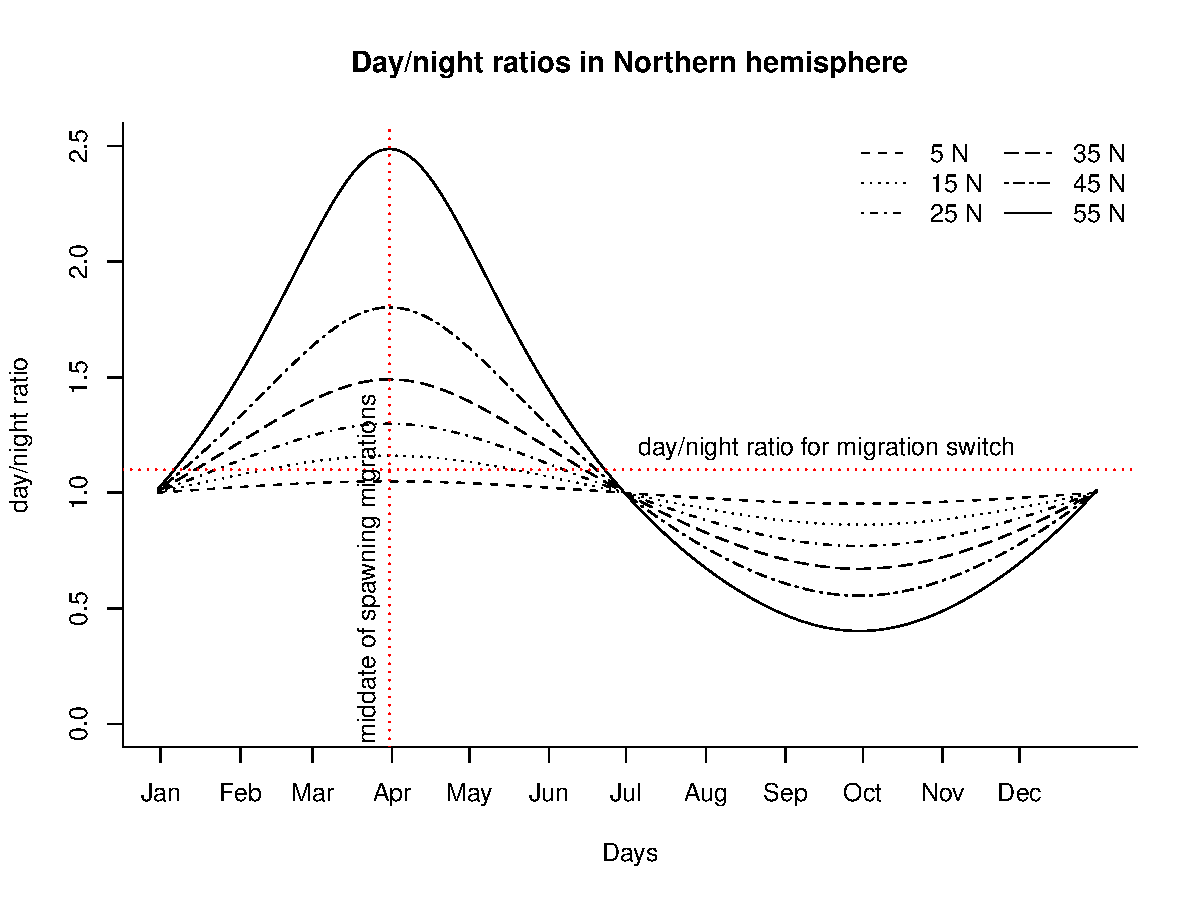
\includegraphics[width=0.75\textwidth]{chapter1/figs/DN-ratio}\\
  \includegraphics[width=0.75\textwidth]{chapter1/figs/seasonal_switch}
  \caption{Illustration of seasonal switch functions: (top) day-night ratio $\varrho$ for northern hemisphere; (bottom) the dates of seasonal switch eq.~\ref{eq:switch-function} between feeding and spawning migrations at different latitudes. The dotted vertical lines denote the mid-date, $\hat{t}$, of the spawning season. The parameter $\varrho_s$ defines the latitude, below which the seasonal switch does not occur. }
  \label{fig:seasonal-switch}
\end{figure}

However, the use of the switch function~\eqref{eq:switch-function} and the linear combination of feeding and spawning habitats~\eqref{eq:seasonal-habitat} may lead to two problems. First, the predefined seasonality of a daylight function does not necessarily align with the timing of albacore migrations to the spawning grounds. Second, when feeding and spawning habitats are characterised by very different oceanographic conditions, which is often the case for the temperate species (e.g. albacore, bluefin tuna), these two habitats, spawning and feeding, do not overlap geographically and hence there are no local cues that may stimulate long-distance migrations to spawning grounds. 

\paragraph{The flexible timing} of the spawning season is enabled by adding a time lag to the day $t^{\bigodot}$ of summer solstice:

\begin{equation}
\delta t=t^{\bigodot}-\hat{t},
\label{eq:season-peak}
\end{equation}

 
\noindent and computing the day length at day $t+\delta t$. So, for the day length $\lambda(t + \delta t,y)$, the $\hat{t}$ becomes the mid-date of the spawning season, also called a season peak. In this case the day length is used only as a convenient periodic function providing the seasonality at every latitude. Note that the choice of mathematical form of the function of day length, $\varrho$, should be done within the MLE approach given that parameters defining the moment of the switch $\varrho_s$, and the mid-date of the spawning season $\hat{t}$ can be effectively estimated from the data (Figure~\ref{fig:seasonal-switch-sigma}). For example, we can use the function of day length, the gradient of the day length, or the day-night ratio $\varrho=\lambda/(24-\lambda)$.


\begin{figure}[htbp]
  \centering
  \includegraphics[width=0.75\textwidth]{chapter1/figs/seasonal_with_sigma}
  \caption{Same as in figure~\ref{fig:seasonal-switch}, but including the variations of standard deviation of the Gaussian thermal function (dashed curve, right y-axis), enabling the local cues (expressed through non-zero gradients of seasonal habitat) for mature adult movements. Parameters of seasonal switch estimated based on fisheries data for south Pacific albacore \citep{Senina2020a}.}
  \label{fig:seasonal-switch-sigma}
\end{figure}

\paragraph{Local gradients} To enable the local cues and hence the non-zero velocities for tunas directed towards the spawning grounds and back to the feeding grounds, the following approach has been implemented. Based on the tuna sensitivity to water temperature and the hypothesis that adult tunas follow warmer temperatures while moving towards maturation and spawning areas \citep{LeGall}, we suggest using thermal gradients as the driver of migrations. In SEAPODYM, the temperature is the common environmental variable to which tunas respond within both feeding and spawning habitats. The thermal preferences at all ages $a \in (0,A^{+})$ are described by Gaussian-type functions with two parameters, ${T_a}^*$ and $\sigma_a$, being the preferred optimum and the temperature tolerance range respectively~\eqref{eq:feeding-thermal}. To link seasonal movements to thermal gradients, we assume that the range of preferred temperatures in the mature tuna’s habitat varies with time. It is maximal at the beginning of migrations, that is, at the moment of the switch, and decreases to the range of temperatures characteristic for the spawning at the seasonal peak. One way to describe this variable $\sigma_{a,s}(t)$ during the spawning season is to relate it linearly to the function of day length $\varrho(t,y_n)$ at a given (fixed to the northernmost) latitude $y_n$, namely to its deviation $\delta \varrho$ from its value at season peak $\varrho (\hat(t),y_n)$:

\begin{equation}
  \sigma_{a,s}=\sigma_0+\left(\bar{\sigma_a}-\sigma_0\right) \frac{\delta \varrho}{\delta \varrho_{max}} 
\label{eq:var-sigma}
\end{equation}

\noindent where $\sigma_0$ is the standard deviation providing a range of preferred temperatures in spawning habitat; $\bar{\sigma_a}={T_0}^*-{T_a}^*$ is the difference between optimal spawning temperatures and preferred temperatures of tunas aged $a$; and $\delta \varrho_{max}$ is the maximum deviation of the chosen day length functions. Note that one standard deviation $\sigma_{a,s}$ being the difference between $H_a$ and $H_s$ thermal optima provides the highest gradients of the Gaussian thermal function. The seasonality of the spawning migrations and variable thermal range $\sigma_{a,s}$ are illustrated in Figure~\ref{fig:seasonal-switch-sigma}. Note that the variability of $\sigma_{a,s}$ is effective only within a spawning season occurring once per year in each hemisphere. 



\subsection{Natural mortality}\label{sec:natural-mortality}

The natural mortality of fish includes two mechanisms --  population decay due to the predation process and population abundance decrease due to senescence of individuals with age, denoted $m_P(a)$ and  $m_S(a)$ , respectively. They are modelled in SEAPODYM by the following equations:

\begin{align}
	m_P(a) = \bar{m}_P e^{-\beta_P a} \label{eq:Mp}\\
	m_S(a)  = \bar{m}_S a^{\beta_S} \label{eq:Ms}
\end{align}
	
\noindent where parameter $\bar{m}_P>0$ is the maximal predation rate, corresponding to age 0 and $\bar{m}_S>0$ is the senescence mortality rate at $a=1$, and $\beta_P>0$ and $\beta_S>0$ define the rates of mortality change with age; their positiveness corresponds to an assumption that predation mortality decreases with age and senescence increases. So the total mortality rate is simply a sum of two terms, predation and senescence mortality (Figure~\ref{fig:mean-mortality}):

\begin{equation}
m(a) = m_P(a)+m_S(a)
\label{eq:M}
\end{equation}

\begin{figure}[htbp]
  \centering
  \includegraphics[width=0.55\textwidth]{chapter1/figs/mortality-func}
  \caption{Total mortality rates due to senescence,$m_S(a)$ eq.~\eqref{eq:Ms}, due to predation, $m_P(a)$ eq.~\eqref{eq:Mp}, the total mortality rate, $m(a)$ eq.~\eqref{eq:M}, as well as the range of variability of mortality rate $m_N$, eq.~(\ref{eq:Mvar}), related to feeding habitat index.}
  \label{fig:mean-mortality}
\end{figure}

In addition, it is assumed that at any age, the natural mortality can be altered by environmental conditions, such as temperature, availability of food and predators. Hence, we assume that total mortality rate $m$ can vary in space and time depending either on the spawning habitat index $H_s$ (for larval and small juvenile stages) or feeding habitat index $H_a$ for adult life stages. Let us denote $I$ the index of habitat occupied by the life stage:

%\begin{displaymath}
\begin{eqnarray}
 I = \left\{
 \begin{array}{cl}
	H_s\text{, if}& a=0\\
	H_j\text{, if}& a \in (0,a_J]  \\
	H_a\text{, if}& a>a_J
  \end{array} 
  \right.
\label{eq:H-in-M}  
\end{eqnarray}
%\end{displaymath}

\noindent where the index $H_j$, used to describe the conditions for survival of juveniles and affecting only the local (in every position $\mathbf{x}$) mortality rates of juveniles, is computed as follows:

\begin{itemize}
\item $H_j=f_1(\Lambda,\alpha) \times f_2(T_1;T^*_0,\sigma_0)$, or
\item same as above but including the density-dependent function accounting for cannibalism by adults. However, this is deliberately left out of the scope of this manual due to weak observability of the mechanism from fisheries data. 
\end{itemize}

\noindent It is important to note that index $H_j$ does not affect movements of juveniles, hence their distribution can be modified by $H_j$ only in case of strong environmental variability and the variable mortality effect estimated by the MLE approach (see chapter~\ref{ch:parametrisation}). 

To account for the effect of environmental conditions on local mortality rates, the mortality at age $m$ in eq.~\ref{eq:M} is affected by the habitat index variability in time and space. Hence the final formulation of a species' natural mortality $m_N=m_N(a,t,\mathbf{x})$ becomes:

	\begin{align}
	m_N & = m(a)(1+\varepsilon)^{1-2I}
	\label{eq:Mvar}
	\end{align}
	
\noindent where $\varepsilon$ is the parameter that gives the range of variability of mortality rate with habitat index within the range $m_N \in [m(a)/(1+\epsilon),m(a)(1+\epsilon)]$ where the minimal value corresponds to the most favourable habitat, $I=1$, and the maximal to the less favourable habitat, $I=0$. 


\subsection{Fishing mortality}\label{sec:FM}
In SEAPODYM, the mortality due to fishing $m_F=m_F(t,a,\mathbf{x})$ is computed based on two methods: 1) using  the Gordon--Schaefer formula and 2) using the catch removal method. The first classical approach relies on the geo-referenced observed fishing effort $E=E(t,\mathbf{x})$ as in the continuous Gordon--Schaefer model, and in the context of age explicit modelling, the mortality rate caused by fishing activity for the part of population at age $a$ is  

\begin{align}
&m_F(a)= q \cdot E \cdot s(a), 
\label{eq:Gordon--Schaefer}
\end{align}

\noindent where $q$ is the catchability of the fishing gear, and $s(a)$ is its selectivity for the fish at age $a$. Note, the fish population is usually harvested with different fishing gears, meaning that the model must consider multiple fisheries, so the catchability coefficient, $q_f$, fishing effort, $E_f$, as well as the gear selectivity, $s_f(a)$, are all fishery dependent. Then the total fishing mortality is computed as a sum of all mortality rates for fisheries being considered:

\begin{align}
&m_F(a)= \sum_f(q_f \cdot E_f \cdot s_f(a)). 
\label{eq:FM}
\end{align}

The selectivity, $s_f(a)$, being a function of age (length), is computed either as a non-linear concave function with a limit one (type I selectivity function), sigmoid function (type II selectivity function) or asymmetric Gaussian (type III):

\begin{eqnarray}
  \label{eq:fishery-specific-selectivity}
  s_{f}(a) = 
  \left\{\begin{array}{lll}
      \frac{\ell(a)}{\varsigma_f+\ell(a)},  & \textrm{  type I} \\
      \left(1+e^{-\varsigma_f (\ell(a)-\hat{l}_f)}\right)^{-1}, 
      & \textrm{  type II} \\
      e^{-\frac{(\ell(a)-\hat{l}_f)^2}{\sigma_{s_f}}}, 
      & \textrm{if $\ell(a)\leq\hat{l}$} \textrm{,  type II,}\\
      \mu_f+(1-\mu_f)e^{-\frac{(\ell(a)-\hat{l}_f)^2}{\sigma_{s_f}}}, 
      & \textrm{if $\ell(a)>\hat{l}$} \textrm{,  type III.} 
  \end{array}\right.
\end{eqnarray}	 


\noindent where
\begin{itemize}
\item $\varsigma_f$ is a half-saturation constant in the selectivity function type I;
\item $\varsigma_f$ is a slope coefficient in sigmoid-shape selectivity;
\item $\hat{l}_f$ and $\sigma_{s_f}$ are the parameters of Gaussian function (mean and standard deviation); and
\item $\mu_f$ is the asymptotic value of selectivity at large fish sizes.
\end{itemize}

\noindent The choice of the functional form of selectivity depends on fishing gear and hence is determined by different factors such as the use of hooks or seine, their depths and mesh size (in case of seine). For example, the sigmoid function is commonly used for long-line fishery, while for purse seine gear, operating at the surface and targeting mostly the younger (smaller) fish, type III is more appropriate (see Figure~\ref{fig:sq-plots}).  

\begin{figure}[htbp]
	\centering
		\includegraphics[width=1.00\textwidth]{chapter1/figs/plots_sq}
	\caption{Catchability and selectivity by fishery estimated for different optimization experiments for south Pacific albacore \citep*[from][]{Senina2020a}. The y-axis shows the product of catchability coefficient (constant in space and time) and selectivity function (varies with size between 0 and 1) so that the plot gives catchability by size. For fisheries for which a dashed line is present, the catchability was allowed to vary linearly in time to account for the change in the gears/strategy efficiency. In that case the dashed lines correspond to the catchability at size at the beginning of the run and the solid lines show the catchability at size at the end of the run.}
	\label{fig:sq-plots}
\end{figure}

The second method, called the \textit{catch removal} method, consists of subtraction of total (summarised over all fisheries) observed catch in number of fish of a given age class directly from the predicted fish density. Note that since catch is by definition a discrete variable, it is more convenient to use discrete notations for this variable as well as for all operators including it. Obviously, catch subtraction occurs only in those locations in space where catch is non-zero. Let us denote all variables in a position of a discretised space, that is, in a grid cell with indices $(i,j)$. 
Subscripts $f,K,p,i,j$ denote fishery, model integration time step index, age index and grid cell indices respectively (notations of Chapter 2~{\hypersetup{linkcolor=black}{\bfseries \nameref{ch:numerics}}}).

Let us denote by $N_{k,p,i,j}$ the population density in number of fish within age class $p$ per unit area at the model integration sub-step $k\frac{\Delta T}{n_t}$ ($k=1,\dots,n_t$, $n_t$ -- number of iterations in the inner loop of ADI method). Quantity $C^{\text{obs}}_{k,p,i,j}=\frac{1}{n_t}C^{\text{obs}}_{K,p,i,j}$ is the $n$th portion of the total observed catch in number of individuals from age class $p$ and time interval $K$. The fishing mortality is accounted through the subtraction (removal) of the observed catch directly from the population density at the ADI method sub-step. To ensure the positivity of the fish population density, it can only be reduced by the amount that corresponds to the sustained catch, that is smaller than the model biomass in a given position in space. Hence, we have the following:

\begin{align}
&N_{k+1,p,i,j} = N_{k,p,i,j}-\text{min}\left(\frac{C_{k,p,i,j}^{\text{obs}}}{\Delta x_i \Delta y}, N_{k,p,i,j}\right),
\label{eq:MCR}
\end{align}

\noindent where a differentiable version of the min function is implemented using a rotated hyperbola in order to avoid a problem of the non-differentiability of the minimum of two values.

Note that the age stratification in catch is usually not available in the observational datasets, but the fraction of observed total catch by age $C_{p,i,j}^{\text{obs}}$ can be derived either from the observed length frequency distributions, or simply using the model fishery selectivity function. Because of scarcity of fine-resolution length frequency data, currently the second method is implemented. The latter means that in the catch removal method even though we use the observed quantities, the mortality induced by a fishery depends on model parameters. For more details on catch prediction and parameter estimation see chapter 4~{\hypersetup{linkcolor=black}{\bfseries \nameref{ch:parametrisation}}}.


\begin{comment}
%\section{Model predictions}\label{sec:model-predictions}
%
%%\subsection{Population biomass}\label{sec:predicted-biomass}
%
%\subsection{Catch}\label{sec:predicted-catch}
%In the current version there are two methods of computing fishing mortality and predicted catch: 1) using Gordon--Schaefer formula and 2) using catch removal method. See the fishing mortality methods in section~\ref{sec:FM} in chapter~\ref{ch:model}. The first method is based on the fishing effort. The mortality due to fishing $F_{fa}$, computed in eq.~\ref{FM}, depends on the catchability, $q_f$, of the fishing gear $f$, its selectivity, $s_{fa}$, for the fish at age $a$, and the observed fishing effort, $E_{f}$. The predicted catch $C^{\text{pred}}$ is then computed based on the geo-referenced observed fishing effort $E$ as follows: 
%
%\begin{align}
%&C^{\text{pred}}_{fatij} = F_{fatij} \cdot N_{atij} \cdot \Delta x_i \Delta y_j 
%\label{eq:GS-catch-prediction}
%\end{align}
%
%where sub-scripts $fatij$ denote fishery, age, time step and grid cell indices respectively; $N_{atij}$ is the abundance of fish and $C^{\text{pred}}_{fatij}$ is the total predicted catch in numbers of fish of age $a$. The total predicted catch of fishery $f$ at time $t$, $C^{pred}_{tfij}$ and in weight of fish, is then computed in the model using observed fishing effort $E_{tfij}$ at location $(i,j)$ by 
%
%\begin{align}
%C^{pred}_{tfij}=q_f E_{tfij} \sum\limits^K_{a=1} s_{fa} w_a N_{aij} \mathit{\scriptstyle\Delta} x \mathit{\scriptstyle\Delta} y,
%\label{eq:catch-in-weight}
%\end{align}
%
%
%\noindent where $w_a$ is the mean weight of fish in the $a$-th cohort.
%
%Thus, predicted catch depends not only on the available fish biomass, but equally depends on the fishing effort, gear catchability and selectivity. In SEAPODYM the selectivity parameters do not vary in space and time and catchability is either constant or allowed to change linearly over time. Therefore, the estimation of population spatial distribution in the MLE approach is essentially driven by the spatio-temporal variations of the biomass and the fishing effort. 
%
%Such approach is correct only in the ideal case, i.e. when the fishing effort is well estimated and fully reported. For gears such as purse-seine the estimation of fishing effort is problematic as one should take into account not only the number of sets which were employed after the fish school has been detected, but also the time the boat spent for active searching. The second variable is often hard to estimate and usually the effort becomes inflated in the principal fishing grounds characterized as zones with highest catches and where the fishing boats spend more time and underestimated in the areas, which are rarely visited by the fishermen. As an example, the observed catch per unit of effort (CPUE) of purse-seine fisheries targeting free schools of skipjack are higher outside of main fishing grounds thus showing a clear density gradient towards their edges. 
%
%To avoid the biases associated with the use of inaccurate fishing effort, another method was implemented (see chapter~\ref{ch:parametrisation} for more details). It consists in removal of total (summarized over all fisheries) catch in number of fish of a given age class directly from the predicted fish density. Let us denote $N_{akij}$ - the population density in number of fish of age $a$ per unit area at the model integration step (inner loop in chapter~\ref{ch:numerics}), $k\frac{\Delta t}{n}$ ($k=1..n$, $n$ - number of iterations in ADI method); $C^{\text{obs}}_{akij}=\frac{1}{n}C^{\text{obs}}_{atij}$ is the n-th portion of the total observed catch at time $t$. Then the corresponding predicted catch at the ADI method sub-step is computed as follows:
%
%
%\begin{align}
%&C^{\text{pred}}_{akij} = \text{min}\left(C_{akij}^{\text{obs}}, (N_{akij} \cdot \Delta x_i \Delta y_j) \right).
%\label{eq:catch-removal}
%\end{align}
%
%
%Note, that according to the eq.~\ref{eq:catch-removal} the predicted catch is either equal or less than the observed one. The later happens only if there is not enough biomass in the grid cell. Finally the predicted total catch is attributed to the fisheries $f$ operating in the cell $ij$ according to their observed ratio, i.e.
%
%\begin{align*}
%C^{\text{pred}}_{fatij} = \frac{C^{\text{obs}}_{fatij}}{\sum_f C^{\text{obs}}_{fatij}} \sum_{k=1}^N C^{\text{pred}}_{akij}
%\label{eq:CR-catch-at-age}
%\end{align*}. 
%
%The use of Eqs.\ref{eq:CR} and \ref{eq:MCR} can be combined with the classical approach~\eqref{eq:FM} by applying the later to selected fisheries, for which the fishing effort can be considered unbiased (long-line and pole-and-line fisheries targeting modelled species). One inconvenience of the catch removal approach is that it cannot combine catch data with different units (e.g., metric tons and numbers of fish).  
%
%
%\subsection{Length frequency}\label{sec:length-frequency}
%
%The length frequency, in other words, the predicted proportion at age $a$ in the catch at time $t$ for fishery $f$ in region $r$ is
%
%  \[ Q^{pred}_{tfar}=\frac{s_{fa} \sum\limits_{i,j \in r} E_{fij} N_{aij}\mathit{\scriptstyle\Delta} x \mathit{\scriptstyle\Delta} y}{\sum\limits^K_{a=1} s_{fa} \left(\sum\limits_{i,j \in r} E_{fij} N_{aij}\mathit{\scriptstyle\Delta} x \mathit{\scriptstyle\Delta} y\right)}
%\]
%
%\noindent where indices $ij \in r$, with region $r$ defined by observations, which are usually given at coarser than model resolution (from $5^{\circ} \times 5^{\circ}$ to $10^{\circ} \times 20^{\circ}$); $\Delta x$ and $\Delta y$ are the spatial resolution of computational grid (see~\ref{ch:numerics} for more details). 

\end{comment}

\section{Model parameters}\label{sec:parameters}
We summarise in Table~\ref{tab:parameters} all model parameters that control the SEAPODYM dynamic processes described in this chapter. Note that biological parameters that are used to compute species' length-at-age, weight-at-age as well as maturity-at-age (section~\ref{sec:sp-biology}), are not included in this table as they are not SEAPODYM parameters and usually estimated in external studies. As described in section~\ref{sec:model-dyn}, all dynamic processes in the model are linked to the environmental variables. In addition, the spatial dynamics (movement) that greatly influences all demographic processes in heterogeneous environments, is modelled explicitly. Therefore, a complex and highly dimensional dynamics can be governed by a limited number of parameters. They are listed in Table~\ref{tab:parameters}: reproduction parameters controlling spawning habitat, $H_s$, and source term, $S$; five parameters of natural mortality, $M$; 12 parameters for feeding habitat, $H_a$; and four parameters of movement rates, among which two control advection rates $v_N$ and two define diffusion rates, $D$. In addition, there are two to four parameters per fishery, which contribute to model dynamics through fishing pressure, the number of them depending on the use of a mortality equation (\ref{eq:FM} or \ref{eq:MCR}) and selectivity function eq.~\ref{eq:fishery-specific-selectivity}. However, fisheries parameters also influence  the model predictions, such as predicted catch-at-age and length frequency of catch. The methods for catch and length frequency data predictions are fully detailed in Chapter~\ref{ch:parametrisation}. 

\begin{longtable}{p{.75cm}p{1.5cm}p{11cm}p{1.5cm}}
\caption{Species dynamic parameters with their notations, definitions and  references\label{tab:parameters}}\\\hline
$\boldsymbol \uptheta$	& \textbf{Eq.}&  \textbf{Description} & \textbf{Units}	\\\hline 
\endfirsthead
%\multicolumn{3}{@{}l}{\ldots continued}\\\hline
\multicolumn{3}{@{}l}{Table 1.3 continued}\\\hline
$\boldsymbol \uptheta$	& \textbf{Eq.}&  \textbf{Description} & \textbf{Units}	\\\hline 
\endhead % all the lines above this will be repeated on every page
\hline
%\multicolumn{3}{r@{}}{continued \ldots}\\
\endfoot
\hline
\endlastfoot
    \multicolumn{4}{c}{\textit{Recruitment}} \\
\hline
    $r$ &(\ref{eq:larvae})  &{Reproduction rate in Beverton--Holt function}&$\text{mo}^{-1}$\\
    $b$ &(\ref{eq:larvae})  & {slope parameter in Beverton--Holt function}&$\text{Nb}^{-1}\text{km}^2$\\\hline
    \multicolumn{4}{c}{\textit{Natural mortality}}\\
\hline
    $\bar{m}_p$ &(\ref{eq:Mp}) & {Predation mortality rate age age $0$}&$\text{mo}^{-1}$\\

    $\beta_p$&(\ref{eq:Mp})& {Slope coefficient in predation mortality} &\\

    $\bar{m}_s$ & (\ref{eq:Ms}) & {Senescence mortality rate at age $0$}&$\text{mo}^{-1-\beta_s}$\\

    $\beta_s$ &(\ref{eq:Ms})   & Slope coefficient in senescence mortality&\\

    $\epsilon$ &(\ref{eq:Mvar}) & {Variability of mortality rate with habitat index from $\frac{M}{(1+\epsilon)}$ in the worst habitat to $M(1+\epsilon))$ in the best habitat} &\\\hline

   \multicolumn{4}{c}{\textit{ Spawning habitat}} \\
\hline
    $\sigma$ &\eqref{eq:spawning-thermal}  & {Standard deviation in temperature Gaussian function of spawning habitat}&$^\circ \text{C}$\\

    $T^{\star}$ & \eqref{eq:spawning-thermal} &{Optimal surface temperature for larvae in spawning habitat definition}&$^\circ \text{C}$\\

    $\alpha$ &\eqref{eq:spawning-prey} & {Prey encounter rate in Holling (type III) function} &$\text{day}^{-1}$\\
    $\alpha_{F}$ &(\ref{eq:spawning-pred})  & Log-normal mean parameter in predator-dependent function & g$\cdot$m$^{-2}$\\
    $\beta_{F}$ &(\ref{eq:spawning-pred})  & Log-normal shape parameter in predator-dependent function &\\
\hline
   \multicolumn{4}{c}{\textit{ Feeding habitat}}\\
\hline   
    $T_0$ & (\ref{eq:temperature-length})& {Preferred temperature for age 0} &$^\circ \text{C}$\\
    $T_m$ & (\ref{eq:temperature-length}) & {Preferred temperature for the oldest adult fish} & $^\circ \text{C}$\\ 
    $\sigma_0$ & (\ref{eq:sigma-weight}) 	 & Standard deviation in temperature Gaussian function for age 0 in feeding habitat& $^\circ \text{C}$\\ 
    $\sigma_m$ & (\ref{eq:sigma-weight}) 	 & Standard deviation in temperature Gaussian function at age A+ &  $^\circ \text{C}$\\       
    $b_T$ &(\ref{eq:temperature-length})& {Allometric power coefficient for thermal preferences at age} &\\
    $\gamma$ &(\ref{eq:oxygen})  & {Slope of the oxygen function in layer accessibility}&\\

    $\hat{O}_2$ &(\ref{eq:oxygen}) 	& {Critical value of dissolved oxygen in the layer}& ml/L\\
    
    $E_{11}$ &(\ref{eq:eF-matrix})& Epipelagic forage scaling factor & m$^2\cdot$g$^{-1}$\\
    $E_{22}$ &(\ref{eq:eF-matrix})& Mesopelagic forage scaling factor & m$^2\cdot$g$^{-1}$\\
    $E_{21}$ &(\ref{eq:eF-matrix})& Migrant mesopelagic forage scaling factor & m$^2\cdot$g$^{-1}$\\
    $E_{33}$ &(\ref{eq:eF-matrix})& Lower mesopelagic forage scaling factor & m$^2\cdot$g$^{-1}$\\
    $E_{32}$ &(\ref{eq:eF-matrix})& Migrant lower mesopelagic forage scaling factor & m$^2\cdot$g$^{-1}$\\
    $E_{31}$ &(\ref{eq:eF-matrix})& Highly migrant lower mesopelagic forage scaling factor & m$^2\cdot$g$^{-1}$\\
\hline
    \multicolumn{4}{c}{\textit{ Adult seasonal migrations}} \\
\hline
    $\hat{t}$ &(\ref{eq:switch-function}) & Mid-date (day of the year) of seasonal spawning migrations of adults &\text{day}\\
    
    $\varrho_s$ &(\ref{eq:season-peak}) & Critical value of day-night ratio, $\varrho$, triggering seasonal migrations& \\
\hline
  \multicolumn{4}{c}{\textit{ Movement}} \\
\hline
    $c$ &\eqref{eq:diffusion} & {Coefficient of diffusion variability with habitat index}&\\
    $\sigma$ &\eqref{eq:diffusion}& {Multiplier for the theoretical diffusion rate $\frac{{\bar{V}}^2 \Delta T}{4}$}& \\
    $V_m$ &\eqref{eq:taxis-coefficient} & {Velocity at maximal habitat gradient and $A=1$, $\text{BL}/\text{s}$}& \\
    $A$ &\eqref{eq:taxis-coefficient} &{Slope coefficient in allometric function for tuna velocity}&\\
\hline
     \multicolumn{4}{c}{\textit{ Fishing mortality and catch prediction}} \\
\hline
    $q_f$ &(\ref{eq:FM},~\ref{eq:catch-in-weight})   & Constant catchability coefficients for all declared fisheries&\\
    $\varsigma_f$ &(\ref{eq:fishery-specific-selectivity})  & Steepness of selectivity function if type I or II, standard deviation if type III&$\text{cm}$\\
    $\hat{l}_f$ & (\ref{eq:fishery-specific-selectivity})  & Threshold length in sigmoid function; mean length in asymmetric Gaussian function &$\text{cm}$ \\
    $\mu_f$ &(\ref{eq:fishery-specific-selectivity}) & Lowest selectivity for large fish in case of asymmetric Gaussian selectivity function&\\		
\hline        
\end{longtable}


\addcontentsline{toc}{section}{References}


\begin{thebibliography}{}

\bibitem[Lehodey et al., 1998]{Lehodey1998} Lehodey P., André J-M., Bertignac M., Hampton J., Stoens A. 1998. Predicting skipjack tuna forage distributions in the Equatorial Pacific using a coupled dynamical bio-geochemical model. \textit {Fisheries Oceanography} 7: 317–325.

\bibitem[Lehodey et al., 2010]{Lehodey2010} Lehodey, P.,  Murtugudde R., Senina I. 2010. Bridging the gap from ocean models to population dynamics of large marine predators: A model of mid-trophic functional groups. \textit{Progress in Oceanography}, Volume 84:69-84.

\bibitem[Lehodey et al., 2015]{Lehodey2015} Lehodey P., Conchon A., Senina I., Domokos R., Calmettes B. et al. 2015. Optimization of a micronekton model with acoustic data. ICES Journal of Marine Research. 53, 571-607. Science 72(5):1399–1412. \url{https:/doi.org/10.1093/icesjms/fsu233}

\end{thebibliography}


\chapter{Discretisation and numerical solution}\label{ch:numerics}

The SEAPODYM underlying partial differential equations (PDE) with initial and boundary conditions eqs.~(\ref{eq:model-1}-\ref{eq:model-3}) are discretised on a regular grid, approximated using the finite-difference method and numerically solved with the alternating-direction implicit (ADI) method \citep{Press}. The numerical approximation scheme and the numerical ADI solver, which are used in SEAPODYM, were developed and implemented by \citet{Sibert-Fournier}  for the general ADR model without an ageing term. It is fully described in \citet{Sibert-Fournier} and \citet{Sibert}. The choice of a classical ADI method despite its known drawbacks, for example, in terms of numerical dispersion, was made for its unconditional stability \citep{Press}, which ensures convergence to a solution for all step sizes and dynamic rates. This method's property enables integration of the numerical model within the optimization method, which implies variations of model parameters. 

The model equations are discretised on a regular Arakawa-A grid. The use of the Arakawa-A grid for the spatial dimensions implies that all quantities are evaluated at the same position, here in the centre of the grid cells. The spatial domain has irregular boundaries. Several boundary conditions are implemented: zero-flux (Neumann) boundary conditions, absorbing (Dirichlet) boundary conditions and conditions for connected east--west borders in the case of a global domain. This chapter describes in detail the discretisation of the model dimensions, the finite-difference approximation of partial derivatives and the numerical solver. 

\section{Discretisation of model dimensions}
\label{sec:discretization}

%\subsection{Discretization of model dimensions}
%\label{sec:dimensions-discretization}

\subsection{Space discretisation}
\label{sec:d-space}

The spatial domain $\Omega\in[X_0,X_m]\times[Y_0,Y_m]$ 
is uniformly discretised in $n_x\times n_y$ cells, 
with a constant step $\Delta x$ (resp. $\Delta y$) along the $x$ (resp. $y$) direction, with the origin $(0,0)$ being the north-west corner of the model domain:

\begin{equation}
  \label{eq:delta-xy}
  \Delta x = (X_m-X_0) / n_x,
  \quad   
  \Delta y = (Y_m-Y_0) / n_y.
\end{equation}
We denote by $(i,j)$, $i=1,\dots n_x$, $j=1,\dots n_y$ the cell that
corresponds to the subdomain 
$[X_0+(i-1)\Delta x,X_0+i\Delta x] \times [Y_0+(j-1)\Delta
  y,Y_0+j\Delta y]$.
All quantities are evaluated at $(x_i,y_j)$, the centre of the cell
$(i,j)$ of the Arakawa-A grid (Figure~\ref{fig:Arakawa-A}), that is
\begin{eqnarray}
  \label{eq:xi}
  x_i &=& X_0+\Big(i-\frac{1}{2}\Big)\Delta x,\quad i=1,\dots, n_x,\\
  \label{eq:yj}
  y_j &=& Y_0+\Big(j-\frac{1}{2}\Big)\Delta y,\quad j=1,\dots, n_y.
\end{eqnarray}


\begin{figure}
   \centering
    \vbox{
    \includegraphics[width=0.5\textwidth]{chapter2/figs/Arakawa-A}
   }
   \caption{Regular Arakawa-A grid used in numerical approximation of SEAPODYM equations. The quantity $N_i=N(x_i,\cdot)$ is the population density described by model eq.~\eqref{eq:model-1}. }
   \label{fig:Arakawa-A}
 \end{figure}

\subsection{Time discretisation}
\label{sec:d-time}

The ADR equation is numerically solved using a multi-incremental algorithm.
The time period $[T_0,T_m]$ is first split into $n_K$ steps or \textbf{outer loops}:
\begin{equation}
  \label{eq:delta-T}
  \Delta T=(T_m-T_0)/n_T,\quad T_K=T_0+K\Delta T,\quad K=0,\dots,n_T.
\end{equation}
where the coefficients of the ADR equation are supposed to be constant. 
Each outer loop is in turn discretised into $n_t$ uniform substeps or \textbf{inner-loops}: 
for a given $K\in\{0,n_T-1\}$ we define
\begin{equation}
  \label{eq:delta-t}
  \Delta t=(T_{K+1}-T_{K})/n_t,\quad t_k=T_{K}+k\Delta t,\quad k=0,\dots,n_t.
\end{equation}
This multi-incremental algorithm is applied with an implicit Euler integration scheme (see below) 
that ensures both stability and good approximation of the solution. 


\subsection{Age discretisation}
\label{sec:d-age}

Population age dimension is discretised into age classes: from the first age class including age $a=0$ to the last age class, including the maximal age $\bar{m}$ of the individuals in the population. In addition, the last age class, also called the $A+$ class, is larger in size than the other age classes. Thus, we define $n_a$ age classes characterized by their age intervals  $[a_p, a_{p+1}]$, $p=0,\dots, n_a$ and the age steps (or age class life period) as follows:
\begin{equation}
  \label{eq:Delta-a}
  \Delta a_p  =a_{p+1} - a_p,\quad p=0,\dots, n_a-1,
\end{equation}
\noindent where the age steps $\Delta a_p = const$ and  $\Delta a_{n_a-1}>\Delta a_p$ for $p=0,\dots, n_a-2$ specify uniformity of all age classes but the last one. Mean age of the age class ${(p)}$ is then given as 
\begin{equation}
  \label{eq:cohort-mean-age}
  \widetilde{a}_{p} = \dfrac{a_{p+1}+a_{p}}{2},\quad p=0,\dots, n_a.
\end{equation}


\begin{table}[!htb]
  \centering
  \begin{tabular}{l|l|l|l|l|l}
    \textbf{Dimension} & \textbf{Variable} & \textbf{Range} & \textbf{Index} & \textbf{Range}  & \textbf{Step}\\
    \hline   \hline                                                                    
    x-coordinate      & $x_i$ & $[X_0,X_m]$      & $i$   & $1,\dots,n_x$ & $\Delta x$ \\\hline
    y-coordinate      & $y_j$ & $[Y_0, Y_m]$     & $j$   & $1,\dots,n_y$ & $\Delta y$ \\\hline
    time (outer loop) & $T_K$ & $[T_0,T_m]$      & $K$   & $0,\dots,n_T$ & $\Delta T$ \\\hline
    time (inner loop) & $t_k$ & $[T_K,T_{K+1}]$  & $k$   & $0,\dots,n_t$ & $\Delta t$ \\\hline
    age               & $a_p$ & $[0,\bar{a}]$    & $p$   & $0,\dots,n_a$ & $\Delta a_p$ \\\hline
    \hline
  \end{tabular}
  \caption{\label{tab:indices}Dimension discretisation indices}
\end{table}

\noindent
\textbf{Notation convention}:
\\
\begin{itemize}
    \item Index names and their meaning are shown in Table \ref{tab:indices}.
    \item For a given quantity $Q$ we define
    \begin{align}
      \label{eq:quantity-grid-tk}
      & Q_{k,p,i,j} = Q(t_k, \widetilde{a}_p, x_i,y_j),&
      \\\nonumber \mbox{and}\\
      \label{eq:quantity-grid-Tk}
      & Q_{K,p,i,j} = Q(T_K, \widetilde{a}_p, x_i,y_j).&
    \end{align}
    \item When there is no loss of clarity we may omit dependence of some variables (or indices). 
\end{itemize}

\section{Approximation of equations and numerical scheme}
\label{sec:equation-discrete-and-numerical-scheme}

The partial derivatives of system (\ref{eq:model-1}-\ref{eq:model-3}) are approximated using centred finite differences. Time integration is performed using a two-step splitting method: advection--diffusion and mortality processes are solved using ADI method along spatial directions: $k\to k+\frac{1}{2}$ for the $x$-direction, $k+\frac{1}{2}\to k+1$ for the $y$-direction. The ageing term is integrated outside of the time integration loop.

During an outer loop period $[T_{K-1},T_{K}]$, we consider that the forcings terms (parameters of advection-diffusion and mortality processes) are constant and equal to their value at $T_{K}$ in order to be consistent with the implicit scheme.

\subsection{Age integration} 
\label{sec:age-integration}

The ageing process is taken into account in between the time integration loops once the solution of the ADR equation is computed over the full time step, that is, between the time steps $[T_{K-1},T_K]$ and $[T_K,T_{K+1}]$ (see also section~\ref{sec:algorithm}). The integration of the ageing term is then done by updating the cohort densities as follows:
\begin{equation}
  \label{eq:aging}
  \left\lbrace
  \begin{array}{lcll}
    N_{K,n_a} &=& N_{K,n_a}+N_{K,n_a-1}&\\
    N_{K,p} &=& N_{K,p-1} &\text{for $p=(n_a-1)\to 1$}
  
  \end{array}
  \right.
\end{equation}


\subsection{Time integration}
\label{sec:two-steps-splitting-method}
%
Time integration from time $T_{K-1}$ to time $T_K$ in the ADI method is done using an iterative \textbf{two-step splitting method along spatial directions}. During these two steps, the ageing process $\partial_a N$ is not taken into account, that is, age class index $p$ is kept constant during time integration.

\paragraph{First half step} \mbox{}\\

\noindent The first implicit half inner-loop time step $k\to k+\frac{1}{2}$ along direction $x$ solves for each inner-loop index $k=0 \dots n_t$:
\begin{align}
  \nonumber
  \dfrac{N_{k+\frac{1}{2}}-N_{k}}{\Delta t/2}
  - \dfrac{\partial}{\partial x}
  \left(
    D_K\dfrac{\partial N_{k+\frac{1}{2}}}{\partial x}
  \right)
  + \dfrac{\partial}{\partial x}
  \left(u_K N_{k+\frac{1}{2}}\right)
  &+ M_{K} N_{k+\frac{1}{2}}
  =\\ \label{eq:2steps-ADI-x}
  &\dfrac{\partial}{\partial y}
  \left(
    D_K\dfrac{\partial N_{k}}{\partial y}
  \right)
  - \dfrac{\partial}{\partial y}
  \left(v_KN_{k}\right).
\end{align}

\paragraph{Second half step} \mbox{}\\
 
\noindent The second implicit  half inner-loop time step $k+\frac{1}{2}\to k+1$ along direction $y$
solves for each inner-loop index $k=0 \dots n_t$:
\begin{align}
  \nonumber
  \dfrac{N_{k+1}-N_{k+\frac{1}{2}}}{\Delta t/2}
  - \dfrac{\partial}{\partial y}
  \left(
    D_K\dfrac{\partial N_{k+1}}{\partial y}
  \right)
  &+ \dfrac{\partial}{\partial y}
  \left(v_KN_{k+1}\right)
  =\\\label{eq:2steps-ADI-y}
  &\dfrac{\partial}{\partial x}
  \left(
    D_K\dfrac{\partial N_{k+\frac{1}{2}}}{\partial x}
  \right)
  - \dfrac{\partial}{\partial x}
  \left(u_KN_{k+\frac{1}{2}}\right)
  - M_{K}N_{k+\frac{1}{2}}.
\end{align}

We then apply discretisation operators \eqref{eq:advection-upwind-x}, \eqref{eq:advection-upwind-y}, \eqref{eq:diffusion-x} and \eqref{eq:diffusion-y} 
depending on the considered cell. For clarity we omit the age class index $p$ in the following paragraphs.

\subsection{Partial derivatives approximation}
\label{sec:ad-derivatives}
\noindent Hereafter we denote by $u$ and $v$ the components of the total velocity 
$\mathbf{v} = \mathbf{v}_c + \mathbf{v}_N$ in eq.~\eqref{eq:model-1}. 

\paragraph{Advection terms}\mbox{} \\

\noindent Derivatives
$\dfrac{\partial}{\partial x}\left( uN \right)$ and 
$\dfrac{\partial}{\partial x}\left( vN \right)$ 
are approximated by centred upwind differencing:
\begin{align}
  \label{eq:advection-upwind-x}
 \left.\dfrac{\partial (uN)}{\partial x}\right|_{i,j} &\approx
 \left\lbrace
   \renewcommand{\arraystretch}{2}
   \begin{array}{lcl}
     \dfrac{1}{\Delta x}(u_{i,j}N_{i,j}-u_{i-1,j}N_{i-1,j}) &
     \mbox{if} & u_{i,j} > 0, \\
     \dfrac{1}{\Delta x}(u_{i+1,j}N_{i+1,j}-u_{i,j}N_{i,j}) &
     \mbox{if} & u_{i,j} < 0, 
   \end{array}
   \right.
   \\
   \label{eq:advection-upwind-y}
   \left.\dfrac{\partial (vN)}{\partial y}\right|_{i,j} &\approx
   \left\lbrace
   \renewcommand{\arraystretch}{2}
   \begin{array}{lcl}
     \dfrac{1}{\Delta y}(v_{i,j}N_{i,j}-v_{i,j-1}N_{i,j-1}) &
     \mbox{if} & v_{i,j} > 0, \\
     \dfrac{1}{\Delta y}(v_{j+1,j}N_{i,j+1}-v_{i,j}N_{i,j}) &
     \mbox{if} & v_{i,j} < 0.
   \end{array}
   \right.
\end{align}

\paragraph{Diffusion terms} \mbox{} \\

\noindent Derivatives
% $ \dfrac{\partial}{\partial x} \left( D\dfrac{\partial N}{\partial x} \right)$ and
% $ \dfrac{\partial}{\partial y} \left( D\dfrac{\partial N}{\partial y} \right)$ 
% are approximated using centered differences on the respective segments $[x_{i-\frac{1}{2}},x_{i+\frac{1}{2}}]$
% and $[y_{j-\frac{1}{2}},y_{j+\frac{1}{2}}]$. The values of $D$ at the boundaries of these segments are approximated by an average 
% (i.e. $D_{i+\frac{1}{2}} \approx (D_{i}+D_{i+1})/2$) \cite{Sibert-1999}: we get:
$\dfrac{\partial}{\partial x} \left( D\dfrac{\partial N}{\partial x} \right)$ and
$ \dfrac{\partial}{\partial y} \left( D\dfrac{\partial N}{\partial y} \right)$ are approximated using centred differences evaluated 
as the mean between the forward finite difference and the backward finite difference of the corresponding terms. We get:
\begin{align}
  %\nonumber
  \left.\dfrac{\partial}{\partial x}\left( D\dfrac{\partial N}{\partial x}\right)\right|_{i,j} 
  &=\left.\dfrac{\partial D}{\partial x}\right|_{i,j} \times \left.\dfrac{\partial N}{\partial x}\right|_{i,j} 
  + D_{i,j}\dfrac{\partial^2 N}{\partial x^2}\\
  &\approx \dfrac{1}{2}\left(
    \dfrac{D_{i+1,j}-D_{i,j}}{\Delta x}\times \dfrac{N_{i+1,j}-N_{i,j}}{\Delta x}\right. \nonumber \\
  &  + \left.\dfrac{D_{i,j}-D_{i-1,j}}{\Delta x}\times \dfrac{N_{i,j}-N_{i-1,j}}{\Delta x}\right) \nonumber\\
  &  + D_{i,j}\times\dfrac{N_{i-1,j}-2N_{i,j}+N_{i+1,j}}{\Delta x^2}\\
%   &\approx\dfrac{1}{\Delta x}\left(
%     D_{i+\frac{1}{2},j} \left.\dfrac{\partial N}{\partial x}\right|_{i+\frac{1}{2},j} -
%     D_{i-\frac{1}{2},j} \left.\dfrac{\partial N}{\partial x}\right|_{i-\frac{1}{2},j}
%    \right)
%    \\
%   &\approx \dfrac{1}{\Delta x}\left(
%       \dfrac{D_{i+1,j}+D_{i,j}}{2}\times\dfrac{N_{i+1,j}-N_{i,j}}{\Delta x}\right.\nonumber \\
%   &-
%       \left.\dfrac{D_{i-1,j}+D_{i,j}}{2}\times\dfrac{N_{i,j}-N_{i-1,j}}{\Delta x}
%     \right)
%     \\
  &\approx
  N_{i-1,j}\dfrac{D_{i,j}+D_{i-1,j}}{2\Delta x^2}
  -N_{i,j}\dfrac{D_{i+1,j}+2D_{i,j}+D_{i-1,j}}{2\Delta x^2} \nonumber\\
  \label{eq:diffusion-x}
  &+  N_{i+1,j}\dfrac{D_{i,j}+D_{i+1,j}}{2\Delta x^2} 
  \\\nonumber\\
  \nonumber
  \left.\dfrac{\partial}{\partial y}\left(
      D\dfrac{\partial N}{\partial y}\right)\right|_{i,j}
  &\approx
  N_{i,j-1}\dfrac{D_{i,j}+D_{i,j-1}}{2\Delta y^2}
  - N_{i,j}\dfrac{D_{i,j+1}+2D_{i,j}+D_{i,j-1}}{2\Delta y^2}
  \\\label{eq:diffusion-y}
  &+ N_{i,j+1}\dfrac{D_{i,j}+D_{i,j+1}}{2\Delta y^2}.
\end{align}


\subsection{Numerical scheme}

For a given grid cell inside the model domain (interior cell), we consider four types of neighbours:
\begin{itemize}
\item ocean cell inside the computation domain,
\item ocean cell outside the computation domain,
\item ocean cell within the East--West overlap zone (in the global domain set-up only),
\item land cell.
\end{itemize}
\vskip 10pt

\noindent Hence, the first three types of interior grid cells are open cells and the last one is the closed boundary cell. Hereafter we provide the model numerical scheme in the interior grid cells; depending whether they are open or closed cells.

\subsubsection{Discretised equations in open grid cells}

In the interior cells surrounded by ocean cells the implicit scheme of eq.~(\ref{eq:2steps-ADI-x}) for the first half time step $k\to k+\frac{1}{2}$ uses spatial terms discretised in the x direction. According to upwind differencing of advection terms, these discrete equations account for the positiveness of $u_{K,i,j}$ and $v_{K,i,j}$:
\begin{itemize}
\item Case $u_{K,i,j}>0$ and $v_{K,i,j}>0$ :
\begin{align}
  \label{eq:2steps-ADI-x-upos-vpos}
  \nonumber
    &N_{k+\frac{1}{2},i-1,j}  \left(
    -\dfrac{u_{K,i-1,j}}{\Delta x}
    -\dfrac{D_{K,i,j}+D_{K,i-1,j}}{2\Delta x^2}
    \right)& \\\nonumber
    &+ N_{k+\frac{1}{2},i,j}  \left(
      \dfrac{2}{\Delta t} 
    +\dfrac{u_{K,i,j}}{\Delta x}
    +\dfrac{D_{K,i+1,j}+2D_{K,i,j}+D_{K,i-1,j}}{2\Delta x^2}
    + M_{K,i,j}    
    \right) \\\nonumber
    & + N_{k+\frac{1}{2},i+1,j} \left(
      -\dfrac{D_{K,i,j}+D_{K,i+1,j}}{2\Delta x^2}
    \right) = \\
    &N_{k,i,j-1}\left(\dfrac{D_{K,i,j}+D_{K,i,j-1}}{2\Delta y^2}+\dfrac{v_{K,i,j-1}}{\Delta y}\right)\\\nonumber
    &+ N_{k,i,j}\left(\dfrac{2}{\Delta t}-\dfrac{v_{K,i,j}}{\Delta y}-\dfrac{D_{K,i,j+1}+2D_{K,i,j}+D_{K,i,j-1}}{2\Delta y^2} \right)
    + N_{k,i,j+1}\left(\dfrac{D_{K,i,j}+D_{K,i,j+1}}{2\Delta y^2}\right)
\end{align}
\item Case $u_{K,i,j}>0$ and $v_{K,i,j}<0$:
\begin{align}
  \label{eq:2steps-ADI-x-upos-vneg}
  \nonumber
    &N_{k+\frac{1}{2},i-1,j}  \left(
    -\dfrac{u_{K,i-1,j}}{\Delta x}
    -\dfrac{D_{K,i,j}+D_{K,i-1,j}}{2\Delta x^2}
    \right)& \\\nonumber
    &+ N_{k+\frac{1}{2},i,j}  \left(
      \dfrac{2}{\Delta t} 
    +\dfrac{u_{K,i,j}}{\Delta x}
    +\dfrac{D_{K,i+1,j}+2D_{K,i,j}+D_{K,i-1,j}}{2\Delta x^2}
    + M_{K,i,j}    
    \right) \\\nonumber
    & + N_{k+\frac{1}{2},i+1,j} \left(
      -\dfrac{D_{K,i,j}+D_{K,i+1,j}}{2\Delta x^2}
    \right) 
    = \\
    \nonumber
    &N_{k,i,j-1}\left(\dfrac{D_{K,i,j}+D_{K,i,j+1}}{2\Delta y^2}\right)
    + N_{k,i,j}\left(\dfrac{2}{\Delta t}+\dfrac{v_{K,i,j}}{\Delta y}-\dfrac{D_{K,i,j+1}+2D_{K,i,j}+D_{K,i,j-1}}{2\Delta y^2} \right)\\
    &+N_{k,i,j+1}\left(\dfrac{D_{K,i,j}+D_{K,i,j+1}}{2\Delta y^2}-\dfrac{v_{K,i,j+1}}{\Delta y}\right)
\end{align}
%
\item Case $u_{K,i,j}<0$ and $v_{K,i,j}>0$:
\begin{align}
  \label{eq:2steps-ADI-x-uneg-vpos}
  \nonumber
    &N_{k+\frac{1}{2},i-1,j}  \left(
      -\dfrac{D_{K,i,j}+D_{K,i-1,j}}{2\Delta x^2}
    \right) \\\nonumber
    &+ N_{k+\frac{1}{2},i,j}  \left(
      \dfrac{2}{\Delta t} 
    -\dfrac{u_{K,i,j}}{\Delta x}
    +\dfrac{D_{K,i+1,j}+2D_{K,i,j}+D_{K,i-1,j}}{2\Delta x^2}
    + M_{K,i,j}    
    \right) \\\nonumber
    &+ N_{k+\frac{1}{2},i+1,j} \left(
      \dfrac{u_{K,i+1,j}}{\Delta x}
      -\dfrac{D_{K,i,j}+D_{K,i+1,j}}{2\Delta x^2}
    \right) 
    = \\
    &N_{k,i,j-1}\left(\dfrac{D_{K,i,j}+D_{K,i,j-1}}{2\Delta y^2}+\dfrac{v_{K,i,j-1}}{\Delta y}\right)\\
    \nonumber
    &+ N_{k,i,j}\left(\dfrac{2}{\Delta t}-\dfrac{v_{K,i,j}}{\Delta y}-\dfrac{D_{K,i,j+1}+2D_{K,i,j}+D_{K,i,j-1}}{2\Delta y^2} \right)
    +N_{k,i,j+1}\left(\dfrac{D_{K,i,j}+D_{K,i,j+1}}{2\Delta y^2}\right)
\end{align}
\item Case $u_{K,i,j}<0$ and $v_{K,i,j}<0$:
\begin{align}
  \label{eq:2steps-ADI-x-uneg-vneg}
  \nonumber
    &N_{k+\frac{1}{2},i-1,j}  \left(
      -\dfrac{D_{K,i,j}+D_{K,i-1,j}}{2\Delta x^2}
    \right) \\\nonumber
    &+ N_{k+\frac{1}{2},i,j}  \left(
      \dfrac{2}{\Delta t} 
    -\dfrac{u_{K,i,j}}{\Delta x}
    +\dfrac{D_{K,i+1,j}+2D_{K,i,j}+D_{K,i-1,j}}{2\Delta x^2}
    + M_{K,i,j}    
    \right) \\\nonumber
    &+ N_{k+\frac{1}{2},i+1,j} \left(
      +\dfrac{u_{K,i+1,j}}{\Delta x}
      -\dfrac{D_{K,i,j}+D_{K,i+1,j}}{2\Delta x^2}
    \right) 
    = \\
    \nonumber
    &N_{k,i,j-1}\left(\dfrac{D_{K,i,j}+D_{K,i,j+1}}{2\Delta y^2}\right)
    + N_{k,i,j}\left(\dfrac{2}{\Delta t}+\dfrac{v_{K,i,j}}{\Delta y}-\dfrac{D_{K,i,j+1}+2D_{K,i,j}+D_{K,i,j-1}}{2\Delta y^2} \right)\\
    &+N_{k,i,j+1}\left(\dfrac{D_{K,i,j}+D_{K,i,j+1}}{2\Delta y^2}-\dfrac{v_{K,i,j+1}}{\Delta y}\right).
\end{align}
\end{itemize}

For the second half time step $k+\frac{1}{2} \to k $, the implicit scheme of eq.~(\ref{eq:2steps-ADI-y}) uses spatial derivatives approximated along the $y$ direction and accounts for the positiveness of $u_{K,i,j}$
and $v_{K,i,j}$
\begin{itemize}
\item Case $v_{K,i,j}>0$ and $u_{K,i,j}>0$:
\begin{align}
  \label{eq:2steps-ADI-y-vpos-upos}
  \nonumber
  &N_{k+1,i,j-1}  \left(
    -\dfrac{v_{K,i,j-1}}{\Delta y}
    -\dfrac{D_{K,i,j}+D_{K,i,j-1}}{2\Delta y^2}
  \right) 
  \\\nonumber
  &+ N_{k+1,i,j}  \left(
    \dfrac{2}{\Delta t} 
    +\dfrac{v_{K,i,j}}{\Delta y}
    +\dfrac{D_{K,i,j+1}+2D_{K,i,j}+D_{K,i,j-1}}{2\Delta y^2}\right) 
  \\\nonumber
  & + N_{k+1,i,j+1} \left(
    -\dfrac{D_{K,i,j}+D_{K,i+1,j}}{2\Delta y^2}
  \right) = 
  \\
  \nonumber
  &N_{k+\frac{1}{2},i-1,j}\left(\dfrac{D_{K,i,j}+D_{K,i-1,j}}{2\Delta x^2}
    +\dfrac{u_{K,i-1,j}}{\Delta x}\right)
  \\\nonumber
  &+ N_{k+\frac{1}{2},i,j}\left(\dfrac{2}{\Delta t}-\dfrac{u_{K,i,j}}{\Delta x}
    -\dfrac{D_{K,i+1,j}+2D_{K,i,j}+D_{K,i-1,j}}{2\Delta x^2}- M_{K,i,j} \right)\\
  &+N_{k+\frac{1}{2},i+1,j}\left(\dfrac{D_{K,i,j}+D_{K,i+1,j}}{2\Delta x^2}\right)
\end{align}
\item Case $v_{K,i,j}>0$ and $u_{K,i,j}<0$:
 \begin{align}
   \label{eq:2steps-ADI-y-vpos-uneg}
    \nonumber
  &N_{k+1,i,j-1}  \left(
    -\dfrac{v_{K,i,j-1}}{\Delta y}
    -\dfrac{D_{K,i,j}+D_{K,i,j-1}}{2\Delta y^2}
  \right) 
  \\\nonumber
  &+ N_{k+1,i,j}  \left(
    \dfrac{2}{\Delta t} 
    +\dfrac{v_{K,i,j}}{\Delta y}
    +\dfrac{D_{K,i,j+1}+2D_{K,i,j}+D_{K,i,j-1}}{2\Delta y^2}\right) 
  \\\nonumber
  & + N_{k+1,i,j+1} \left(
    -\dfrac{D_{K,i,j}+D_{K,i+1,j}}{2\Delta y^2}
  \right) = 
  \\
  \nonumber
  &N_{k+\frac{1}{2},i-1,j}\left(\dfrac{D_{K,i,j}+D_{K,i-1,j}}{2\Delta x^2}\right)
  \\\nonumber
  &+ N_{k+\frac{1}{2},i,j}\left(\dfrac{2}{\Delta t}+\dfrac{u_{K,i,j}}{\Delta x}
    -\dfrac{D_{K,i+1,j}+2D_{K,i,j}+D_{K,i-1,j}}{2\Delta x^2}- M_{K,i,j} \right)\\
  &+N_{k+\frac{1}{2},i+1,j}\left(\dfrac{D_{K,i,j}+D_{K,i+1,j}}{2\Delta x^2}
  -\dfrac{u_{K,i+1,j}}{\Delta x}\right)
 \end{align}
\item Case $v_{K,i,j}<0$ and $u_{K,i,j}>0$:
\begin{align}
  \label{eq:2steps-ADI-y-vneg-upos}
  \nonumber
  &N_{k+1,i,j-1}  \left(
    -\dfrac{D_{K,i,j}+D_{K,i,j-1}}{2\Delta y^2}
  \right) 
  \\\nonumber
  &+ N_{k+1,i,j}  \left(
    \dfrac{2}{\Delta t} 
    -\dfrac{v_{K,i,j}}{\Delta y}
    +\dfrac{D_{K,i,j+1}+2D_{K,i,j}+D_{K,i,j-1}}{2\Delta y^2}\right) 
  \\\nonumber
  & + N_{k+1,i,j+1} \left(
    -\dfrac{D_{K,i,j}+D_{K,i+1,j}}{2\Delta y^2}
    +\dfrac{v_{K,i,j+1}}{\Delta y}
  \right) = 
  \\
  \nonumber
  &N_{k+\frac{1}{2},i-1,j}\left(\dfrac{D_{K,i,j}+D_{K,i-1,j}}{2\Delta x^2}
    +\dfrac{u_{K,i-1,j}}{\Delta x}\right)
  \\\nonumber
  &+ N_{k+\frac{1}{2},i,j}\left(\dfrac{2}{\Delta t}-\dfrac{u_{K,i,j}}{\Delta x}
    -\dfrac{D_{K,i+1,j}+2D_{K,i,j}+D_{K,i-1,j}}{2\Delta x^2}- M_{K,i,j} \right)\\
  &+N_{k+\frac{1}{2},i+1,j}\left(\dfrac{D_{K,i,j}+D_{K,i+1,j}}{2\Delta x^2}\right)
\end{align}
\item Case $v_{K,i,j}<0$ and $u_{K,i,j}<0$:
\begin{align}
  \label{eq:2steps-ADI-y-vneg-uneg}
  \nonumber
  &N_{k+1,i,j-1}  \left(
    -\dfrac{D_{K,i,j}+D_{K,i,j-1}}{2\Delta y^2}
  \right) 
  \\\nonumber
  &+ N_{k+1,i,j}  \left(
    \dfrac{2}{\Delta t} 
    -\dfrac{v_{K,i,j}}{\Delta y}
    +\dfrac{D_{K,i,j+1}+2D_{K,i,j}+D_{K,i,j-1}}{2\Delta y^2}\right) 
  \\\nonumber
  & + N_{k+1,i,j+1} \left(
    -\dfrac{D_{K,i,j}+D_{K,i+1,j}}{2\Delta y^2}
    +\dfrac{v_{K,i,j+1}}{\Delta y}
  \right) = 
  \\
  \nonumber
  &N_{k+\frac{1}{2},i-1,j}\left(\dfrac{D_{K,i,j}+D_{K,i-1,j}}{2\Delta x^2}\right)
  \\\nonumber
  &+ N_{k+\frac{1}{2},i,j}\left(\dfrac{2}{\Delta t}+\dfrac{u_{K,i,j}}{\Delta x}
    -\dfrac{D_{K,i+1,j}+2D_{K,i,j}+D_{K,i-1,j}}{2\Delta x^2}- M_{K,i,j} \right)\\
  &+N_{k+\frac{1}{2},i+1,j}\left(\dfrac{D_{K,i,j}+D_{K,i+1,j}}{2\Delta x^2}
  -\dfrac{u_{K,i+1,j}}{\Delta x}\right)
\end{align}
\end{itemize}

\subsubsection{Discretised equations in closed grid cells}
\label{sec:boundary-conditions}

We now write down the model numerical scheme in closed grid cells, that is, neighbouring with either a land or ocean grid cell assigned as a boundary cell considering three types of boundary conditions: 1) Neumann boundary conditions, 2) Dirichlet boundary conditions, and 3) a special case of Dirichlet boundary conditions in the case of the global domain. 

\paragraph{1) Neumann boundary conditions} \mbox{}\\

\noindent Neumann boundary conditions specify impermeability of domain boundaries. These conditions are applied in the case of closed cells, that is, neighbouring with either land cells or ocean cells, for which impenetrability can be assumed due to natural causes. 

Let's use the case of a \textit{left-closed boundary in the $x$-direction and open boundaries in the $y$-direction} in eq.~\eqref{eq:2steps-ADI-x-upos-vpos}: we have 
$N_{k+\frac{1}{2},i-1,j}= N_{k+\frac{1}{2},i,j}$, $D_{K,i-1,j}=0$ and 
$u_{K,i-1,j}=0$. 
Then if $u_{K,i,j}>0$ and $v_{K,i,j}>0$ we get
\begin{align}
  \label{eq:2steps-ADI-x-upos-vpos+Neumann}
  \nonumber
    &N_{k+\frac{1}{2},i,j}  \left(
      \dfrac{2}{\Delta t} 
    +\dfrac{u_{K,i,j}}{\Delta x}
    +\dfrac{D_{K,i+1,j}+D_{K,i,j}}{2\Delta x^2}
    + M_{K,i,j}    
    \right)
    + N_{k+\frac{1}{2},i+1,j} \left(
      -\dfrac{D_{K,i,j}+D_{K,i+1,j}}{2\Delta x^2}
    \right) 
    = \\
    \nonumber
    &N_{k,i,j-1}\left(\dfrac{D_{K,i,j}+D_{K,i,j-1}}{2\Delta y^2}+\dfrac{v_{K,i,j-1}}{\Delta y}\right)
    + N_{k,i,j}\left(\dfrac{2}{\Delta t}-\dfrac{v_{K,i,j}}{\Delta y}-\dfrac{D_{K,i,j+1}+2D_{K,i,j}+D_{K,i,j-1}}{2\Delta y^2} \right)\\
    &+N_{k,i,j+1}\left(\dfrac{D_{K,i,j}+D_{K,i,j+1}}{2\Delta y^2}\right)
\end{align}
%
Also if $u_{K,i,j}<0$ and $v_{K,i,j}>0$ we get
%
\begin{align}
  \label{eq:2steps-ADI-x-uneg-vpos+Neumann}
  \nonumber
    &N_{k+\frac{1}{2},i,j}  \left(
      \dfrac{2}{\Delta t} 
    +\dfrac{D_{K,i+1,j}+D_{K,i,j}}{2\Delta x^2}
    + M_{K,i,j}    
    \right)
    + N_{k+\frac{1}{2},i+1,j} \left(
      \dfrac{u_{K,i+1,j}}{\Delta x}
      -\dfrac{D_{K,i,j}+D_{K,i+1,j}}{2\Delta x^2}
    \right) 
    = \\
    \nonumber
    &N_{k,i,j-1}\left(\dfrac{D_{K,i,j}+D_{K,i,j-1}}{2\Delta y^2}+\dfrac{v_{K,i,j-1}}{\Delta y}\right)
    + N_{k,i,j}\left(\dfrac{2}{\Delta t}-\dfrac{v_{K,i,j}}{\Delta y}-\dfrac{D_{K,i,j+1}+2D_{K,i,j}+D_{K,i,j-1}}{2\Delta y^2} \right)\\
    &+N_{k,i,j+1}\left(\dfrac{D_{K,i,j}+D_{K,i,j+1}}{2\Delta y^2}\right).
\end{align}

\paragraph{2) Dirichlet boundary conditions} \mbox{}\\

\noindent Dirichlet conditions specify the value that a model variable should take at the boundary. This value can be zero (absorbing boundary) to imply the loss of quantity, or non-zero to account for the incoming quantity  from outside the domain. Dirichlet boundary conditions are applied in the case of a regional domain. 
 
Let us take the case of a \textit{left-open-to-global boundary in the $x$-direction and open boundaries in the $y$-direction} in eq.~\eqref{eq:2steps-ADI-x-upos-vpos}: we have 
%$N_{k+\frac{1}{2},i-1,j}= N^{glo}_{k+\frac{1}{2},i-1,j}$ 
$N_{k+\frac{1}{2},i-1,j} = 0$ 
and the corresponding contribution is part of the second member of the equation. For example, if $u_{K,i,j}>0$ and $v_{K,i,j}>0$ we have
\begin{align}
  \label{eq:2steps-ADI-x-upos-vpos+Dirichlet}
  \nonumber
  &N_{k+\frac{1}{2},i,j}  \left(
    \dfrac{2}{\Delta t} 
    +\dfrac{u_{K,i,j}}{\Delta x}
    +\dfrac{D_{K,i+1,j}+2D_{K,i,j}+D_{K,i-1,j}}{2\Delta x^2}
    + M_{K,i,j}    
    \right) \\ \nonumber
    &+ N_{k+\frac{1}{2},i+1,j} \left(
      -\dfrac{D_{K,i,j}+D_{K,i+1,j}}{2\Delta x^2}
    \right) 
    = \\
    \nonumber
    &N_{k,i,j-1}\left(\dfrac{D_{K,i,j}+D_{K,i,j-1}}{2\Delta y^2}+\dfrac{v_{K,i,j-1}}{\Delta y}\right)
    + N_{k,i,j}\left(\dfrac{2}{\Delta t}-\dfrac{v_{K,i,j}}{\Delta y}-\dfrac{D_{K,i,j+1}+2D_{K,i,j}+D_{K,i,j-1}}{2\Delta y^2} \right)\\
    &+N_{k,i,j+1}\left(\dfrac{D_{K,i,j}+D_{K,i,j+1}}{2\Delta y^2}\right).
    % Comment when N^{glo}=0
    % -N^{glo}_{k+\frac{1}{2},i-1,j}  \left(
    % -\dfrac{u_{K,i-1,j}}{\Delta x}
    % -\dfrac{D_{K,i,j}+D_{K,i-1,j}}{2\Delta x^2}
    % \right)
\end{align}

\paragraph{3) Global domain} \mbox{}\\

\noindent In case of a global domain, namely, the domain covering $360^{\circ}$ in a longitudinal direction, we need to take into account fluxes that come through the western (eastern) boundary from the east (west) of the domain. A special case of \textit{cyclic east--west boundary conditions} is implemented in the SEAPODYM numerical scheme. To make sure that the quantity flows through the open east--west boundaries in the context of the ADI method, we extend the computational domain on both sides along the $x$ (longitudinal) direction to create the buffer zone. The eastern (western) buffer zone is then filled with values from the west (east) of the domain. The size of the buffer zone is defined as large enough to cover the maximal distance of the mass movement during one outer time step $[T_{K-1},T_K]$. The discretised equation is then solved on this extended domain, while at the end of the resolution, we only keep the solution over the non-extended part of the domain.

\section{Tridiagonal matrix system and its resolution} 

\noindent The above numerical scheme eqs.~(\ref{eq:2steps-ADI-x-upos-vpos}--\ref{eq:2steps-ADI-x-upos-vpos+Dirichlet}) can be rewritten in matrix form with the matrices on the left-hand side being tridiagonal. For clarity, we use all dimensional notations here, even though the age index $p$ remains constant within the resolution of linear system. Thus, to get the numerical solution of model~(\ref{eq:model-1}) at a given time step, we solve iteratively (inner loop) two systems of linear equations, and each iteration implies resolution of $n_a\times n_y$ and $n_a\times n_x$ systems of linear equations in a two-step time splitting ADI method. 

Thus, at the first half-step we solve $n_a\times n_y$ linear systems of size $n_x\times n_x$ along the $x$-direction:

\begin{align}
\label{eq:matrix-form-x}
 \mathbf{A}_{K,p,j} \cdot \mathbf{N}_{k+\frac{1}{2},p,j} = \mathbf{g}_{k,p,j}
\end{align}

\noindent and then at the second half-step we solve $n_a\times n_x$ linear systems of size $n_y\times n_y$ along the $y$-direction: 

\begin{align}
\label{eq:matrix-form-y}
 \mathbf{B}_{K,p,i} \cdot \mathbf{N}_{k+1,p,i} = \mathbf{h}_{k+\frac{1}{2},p,i}.
\end{align}   

\noindent Vectors $\mathbf{N}_{k+\frac{1}{2},p,j}=(N_{k+\frac{1}{2},p,1,j},\dots,N_{k+\frac{1}{2},p,n_x,j})^{\text{T}}$ and $\mathbf{N}_{k+1,p,i}=(N_{k+1,p,i,1},\dots,N_{k+1,p,i,n_y})^{\text{T}}$ consist of unknown values of population density along the $x$ and $y$ dimensions respectively. These values are found by solving these linear systems with the help of the forward--backward Gauss elimination (LU decomposition) method. 

The right-hand-side vectors $\mathbf{g}_{k,p,j}=(g_{k,p,1,j},\dots,g_{k,p,n_x,j})^{\text{T}}$ in system~\eqref{eq:matrix-form-x}, and $\mathbf{h}_{k+\frac{1}{2},p,i}=(h_{k+\frac{1}{2},p,i,1},\dots,h_{k+\frac{1}{2},p,i,n_y})^{\text{T}}$ in system~\eqref{eq:matrix-form-y} are constructed either from previous step solution, at $K-1$ (for $k=0$), or from an intermediate solution of the Gauss method, at all $k=1,\dots,n_t$, obtained after each iteration of inner loop of the ADI method. Thus, the elements of vector $\mathbf{g}_{k,p,j}$ are computed for given $a=1,\dots,n_a$ and $j=1,\dots,n_y$ from the coefficients of the matrix $\mathbf{B}$ and density at time $k$ as follows:
\begin{equation}
  \label{eq:second-members-x}
  g_{k,p,i,j} = 
  - d_{K,p,i,j}N_{k,p,i,j-1}
  + \left( \dfrac{4}{\Delta t} - e_{K,p,i,j}\right)N_{k,p,i,j} 
  - f_{k,p,i,j}N_{k,p,i,j+1}.
\end{equation}

\noindent The elements of vector $\mathbf{h}_{k+\frac{1}{2},p,i}$ are computed for given $p=0,\dots,n_a$ and $i=1,\dots,n_x$ from the coefficients of the matrix $\mathbf{A}$ and density at time $k+\frac{1}{2}$ as follows:
\begin{equation}
  \label{eq:second-members-y}
  h_{k+\frac{1}{2},p,i,j} = 
  -a_{K,p,i,j}N_{k+\frac{1}{2},p,i-1,j}
  +\left(\frac{4}{\Delta t}-b_{K,p,i,j}\right)N_{k+\frac{1}{2},p,i,j}
  -c_{K,p,i,j}N_{k+\frac{1}{2},p,i+1,j}.
\end{equation}

\noindent Matrix $\mathbf{A}$ of the linear system~\eqref{eq:matrix-form-x} is defined for all $p=1,\dots,n_a$ and for all $j=1,\dots,n_y$ as follows \citep*[notations of][]{Sibert-Fournier}:
\begin{equation}
  \label{eq:A-matrix}
  \mathbf{A}_{K,p,j}=\left(
    \begin{array}{cccccc}
      b_{K,p,1,j} & c_{K,p,1,j} & 0 & \ldots & 0 & 0\\
      a_{K,p,2,j} & b_{K,p,2,j} & c_{K,p,2,j} & 0 & \ldots & 0\\
      0 & a_{K,p,3,j} & b_{K,p,3,j} & c_{K,p,3,j} & \ldots & 0\\
      \vdots & \ddots & \ddots & \ddots & \ddots & \vdots\\
      0 & \ldots & \ldots & a_{K,p,n_x-1,j} & b_{K,p,n_x-1,j}\ & c_{K,p,n_x-1,j}\\
      0 & \ldots & \ldots & 0 & a_{K,p,n_x,j} & b_{K,p,n_x,j}
    \end{array}
  \right).
\end{equation}

\noindent Matrix $\mathbf{B}$ of the linear system~\eqref{eq:matrix-form-y} is defined for all $p=1,\dots,n_a$, and for all $i=1,\dots,n_x$ as follows:
\begin{equation}
  \label{eq:B-matrix}
  \mathbf{B}_{K,p,i}=\left(
    \begin{array}{cccccc}
      e_{K,p,i,1} & f_{K,p,i,1} & 0 & \ldots & 0 & 0\\
      d_{K,p,i,2} & e_{K,p,i,2} & f_{K,p,i,2} & 0 & \ldots & 0\\
      0 & d_{K,p,i,3} & e_{K,p,i,3} & f_{K,p,i,3} & \ldots & 0\\
      \vdots & \ddots & \ddots & \ddots & \ddots & \vdots\\
      0 & \ldots & \ldots & d_{K,p,i,n_y-1} & e_{K,p,i,n_y-1}\ & f_{K,p,i,n_y}\\
      0 & \ldots & \ldots & 0 & d_{K,p,i,n_y} & e_{K,p,i,n_y}\\
    \end{array}
  \right).
\end{equation}

Below we provide the diagonal coefficients of matrices $\mathbf{A}$ and $\mathbf{B}$ given the type of the boundary conditions. 

\subsection{Diagonal coefficients for Neumann boundary conditions} \mbox{}\\

For a given $p=1,\dots,n_a$ and $j=1,\dots,n_y$, the elements of matrix $\mathbf{A}_{K,p,j}$ are\footnote{Note that the diagonal coefficient of matrix $\mathbf{A}$, $a_{K,p,i,j}$, which is always written with four dimensional indices, should not be confused with age notation $a$, nor with discrete age intervals $a_p$.}
 \begin{align}
   \label{eq:matrix-elements-lowerdiag-x}
   a_{K,p,i,j} &= \left\lbrace
     \renewcommand{\arraystretch}{2.5}
     \begin{array}{lll}
       -\dfrac{u_{K,p,i-1,j}}{\Delta x}
       -\dfrac{D_{K,p,i,j}+D_{K,p,i-1,j}}{2\Delta x^2}
       &\mbox{\minitab{open}{right closed}} & u_{K,p,i,j} > 0 \\
       -\dfrac{D_{K,p,i,j}+D_{K,p,i-1,j}}{2\Delta x^2}
       &\mbox{\minitab{open}{right closed}} & u_{K,p,i,j} < 0\\
       0 & \mbox{\minitab{left closed}{}} & 
     \end{array}
     \right.
     \\
     \label{eq:matrix-elements-diag-x}
     b_{K,p,i,j} &=
     \left\lbrace
     \renewcommand{\arraystretch}{2.5}
     \begin{array}{lll}
       \dfrac{2}{\Delta t} 
       +\dfrac{u_{K,p,i,j}}{\Delta x}
       +\dfrac{D_{K,p,i+1,j}+2D_{K,p,i,j}+D_{K,p,i-1,j}}{2\Delta x^2}\\
       + M_{K,p,i,j}    
       &\mbox{open} 
       & u_{K,p,i,j} > 0 \\
       \dfrac{2}{\Delta t} 
       -\dfrac{u_{K,p,i,j}}{\Delta x}
       +\dfrac{D_{K,p,i+1,j}+2D_{K,p,i,j}+D_{K,p,i-1,j}}{2\Delta x^2}\\
       + M_{K,p,i,j}    
       &\mbox{open} & u_{K,p,i,j} < 0\\
       \dfrac{2}{\Delta t} 
       +\dfrac{D_{K,p,i,j}+D_{K,p,i-1,j}}{2\Delta x^2}
       + M_{K,p,i,j}    
       & \mbox{right closed} & u_{K,p,i,j} > 0\\
       \dfrac{2}{\Delta t} 
       -\dfrac{u_{K,p,i,j}}{\Delta x}
       +\dfrac{D_{K,p,i,j}+D_{K,p,i-1,j}}{2\Delta x^2}
       + M_{K,p,i,j}    
       & \mbox{right closed} & u_{K,p,i,j} < 0\\
         \dfrac{2}{\Delta t} 
         +\dfrac{D_{K,p,i+1,j}+D_{K,p,i,j}}{2\Delta x^2}
         + M_{K,p,i,j}    
       &\mbox{left closed} & u_{K,p,i,j} < 0\\
         \dfrac{2}{\Delta t} 
         + \dfrac{u_{K,p,i,j}}{\Delta x}
         +\dfrac{D_{K,p,i+1,j}+D_{K,p,i,j}}{2\Delta x^2}
         + M_{K,p,i,j}    
       &\mbox{left closed} & u_{K,p,i,j} > 0\\
       \dfrac{2}{\Delta t} + M_{K,p,i,j}
       & \mbox{closed}
     \end{array}
   \right.
   \\
   \label{eq:matrix-elements-upperdiag-x}
   c_{K,p,i,j} &=
     \left\lbrace
     \renewcommand{\arraystretch}{2.5}
     \begin{array}{lll}
        \left(
      -\dfrac{D_{K,p,i,j}+D_{K,p,i+1,j}}{2\Delta x^2}
    \right) 
       &\mbox{\minitab{open}{left closed}} & u_{K,p,i,j} > 0 \\
       \left(
         \dfrac{u_{K,p,i+1,j}}{\Delta x}
         -\dfrac{D_{K,p,i,j}+D_{K,p,i+1,j}}{2\Delta x^2}
       \right) 
       &\mbox{\minitab{open}{left closed}} & u_{K,p,i,j} < 0\\
       0 & \mbox{\minitab{right closed}{}} & 
     \end{array}
   \right.
 \end{align}
For a given $i=1,\dots,n_x$ elements of $\mathbf{B}_{K,p,i}$ are given by
 \begin{align}
   \label{eq:matrix-elements-lowerdiag-y}
   d_{K,p,i,j} &= \left\lbrace
     \renewcommand{\arraystretch}{2.5}
     \begin{array}{lll}
       -\dfrac{v_{K,p,i,j-1}}{\Delta y}
       -\dfrac{D_{K,p,i,j}+D_{K,p,i,j-1}}{2\Delta y^2}
       &\mbox{\minitab{open}{bottom closed}} & v_{K,p,i,j} > 0 \\
       -\dfrac{D_{K,p,i,j}+D_{K,p,i,j-1}}{2\Delta y^2}
       &\mbox{\minitab{open}{bottom closed}} & v_{K,p,i,j} < 0\\
       0 & \mbox{\minitab{top closed}{}} & 
     \end{array}
     \right.
     \\
     \label{eq:matrix-elements-diag-y}
     e_{K,p,i,j} &=
     \left\lbrace
     \renewcommand{\arraystretch}{2.5}
     \begin{array}{lll}
       \dfrac{2}{\Delta t} 
       +\dfrac{v_{K,p,i,j}}{\Delta y}
       +\dfrac{D_{K,p,i,j+1}+2D_{K,p,i,j}+D_{K,p,i,j-1}}{2\Delta y^2}\\
       + M_{K,p,i,j}    
       &\mbox{open} & v_{K,p,i,j} > 0 \\
       \dfrac{2}{\Delta t} 
       -\dfrac{v_{K,p,i,j}}{\Delta y}
       +\dfrac{D_{K,p,i,j+1}+2D_{K,p,i,j}+D_{K,p,i,j-1}}{2\Delta y^2}\\
       + M_{K,p,i,j}    
       &\mbox{open} & v_{K,p,i,j} < 0\\
       \dfrac{2}{\Delta t} 
       +\dfrac{D_{K,p,i,j}+D_{K,p,i,j-1}}{2\Delta y^2}
       + M_{K,p,i,j}    
       & \mbox{bottom closed} & v_{K,p,i,j} > 0\\
       \dfrac{2}{\Delta t} 
       -\dfrac{v_{K,p,i,j}}{\Delta y}
       +\dfrac{D_{K,p,i,j}+D_{K,p,i,j-1}}{2\Delta y^2}
       + M_{K,p,i,j}    
       & \mbox{bottom closed} & v_{K,p,i,j} < 0\\
         \dfrac{2}{\Delta t} 
         +\dfrac{v_{K,p,i,j}}{\Delta y}
         +\dfrac{D_{K,p,i,j+1}+D_{K,p,i,j}}{2\Delta y^2}
         + M_{K,p,i,j}    
       &\mbox{top closed} & v_{K,p,i,j} > 0\\
         \dfrac{2}{\Delta t} 
         +\dfrac{D_{K,p,i,j+1}+D_{K,p,i,j}}{2\Delta y^2}
         + M_{K,p,i,j}    
       &\mbox{top closed} & v_{K,p,i,j} < 0\\
       \dfrac{2}{\Delta t} + M_{K,p,i,j}
       &  \mbox{closed}
     \end{array}
   \right.
   \\
   \label{eq:matrix-elements-upperdiag-y}
   f_{K,p,i,j} &=
     \left\lbrace
     \renewcommand{\arraystretch}{2.5}
     \begin{array}{lll}
        \left(
      -\dfrac{D_{K,p,i,j}+D_{K,p,i,j+1}}{2\Delta y^2}
    \right) 
       &\mbox{\minitab{open}{top closed}} & v_{K,p,i,j} > 0 \\
       \left(
         \dfrac{v_{K,p,i,j+1}}{\Delta y}
         -\dfrac{D_{K,p,i,j}+D_{K,p,i,j+1}}{2\Delta y^2}
       \right) 
       &\mbox{\minitab{open}{top closed}} & v_{K,p,i,j} < 0\\
       0 & \mbox{\minitab{bottom closed}{}} & 
     \end{array}
   \right.
 \end{align}

\subsection{Diagonal coefficients for Dirichlet boundary conditions}

\noindent Let us provide the general formulae for movement rates as well as for diagonal coefficients of tridiagonal matrices of linear system that take into account Dirichlet boundary conditions.

First, we define the following expressions to account for the type of neighbouring grid cell
\begin{align}
  \label{eq:global-flag}
  L^g_{i,j} &= \left\lbrace
    \begin{array}{lll}
      1 &\mbox{if} & \mbox{left open-to-global}\\
      0 & \mbox{else}
    \end{array}
  \right.\\
  R^g_{i,j} &= \left\lbrace
    \begin{array}{lll}
      1 &\mbox{if} & \mbox{right open-to-global}\\
      0 & \mbox{else}
    \end{array}
  \right.
\end{align}
We define the movement rates given the closed boundary
\begin{equation}
  \begin{array}{lcll}
    D_{K,p,i-1,j} &=& -D_{K,p,i,j} 
    & \mbox{left-closed}\\
    D_{K,p,i+1,j} &=& -D_{K,p,i,j} 
    & \mbox{right-closed}\\
    u_{K,p,i-1,j} &=& 0
    & \mbox{left-closed}\\
    u_{K,p,i+1,j} &=& 0
    & \mbox{right-closed}\\
    u_{K,p,i,j} &=&
    \max(u_{K,p,i,j},0)
    & \mbox{left-closed}\\
    u_{K,p,i,j} &=&
    \min(u_{K,p,i,j},0)
    & \mbox{right-closed}
  \end{array}
\end{equation}
We update the expressions including finite differences as follows
\begin{eqnarray}
  \label{eq:alpha}
  \alpha_{K,p,i,j} &= -\dfrac{\mbox{sign}(u_{K,p,i-1,j})+1}{2}
  \times\dfrac{u_{K,p,i-1,j}}{\Delta x}
   -\dfrac{D_{K,p,i,j}+D_{K,p,i-1,j}}{2\Delta x^2}\\
   \gamma_{K,p,i,j} & = \dfrac{1-\mbox{sign}(u_{K,p,i+1,j})}{2}
   \times\dfrac{u_{K,p,i+1,j}}{\Delta x}
   -\dfrac{D_{K,p,i,j}+D_{K,p,i+1,j}}{2\Delta x^2}
\end{eqnarray}
Hence, with Dirichlet boundary conditions diagonal coefficients become
\begin{align}
   \label{eq:matrix-elements-lowerdiag-x-general}
   a_{K,p,i,j} &= \alpha_{K,p,i,j}\times(1-L^g_{i,j})
   \\
   \label{eq:matrix-elements-diag-x-general}
   b_{K,p,i,j} &=
   \dfrac{2}{\Delta t}+\mbox{sign}(u_{K,p,i,j})\dfrac{u_{K,p,i,j}}{\Delta x}\\\nonumber
   &+\alpha_{K,p,i,j}\times L^g_{i,j} + \gamma_{K,p,i,j}\times R^g_{i,j}\\\nonumber
   &+\dfrac{D_{K,p,i+1,j}+2D_{K,p,i,j}+D_{K,p,i-1,j}}{2\Delta x^2}+M_{K,p,i,j}
   \\
   \label{eq:matrix-elements-upperdiag-x-general}
   c_{K,p,i,j} &= \gamma_{K,p,i,j}\times(1-R^g_{i,j})
 \end{align}

Similar expressions can be obtained for the coefficients of matrix $B$. The same formulas for the right-hand-side vector elements as eq.~(\ref{eq:second-members-x}) and eq.~(\ref{eq:second-members-y}) are simply updated with Dirichlet boundary conditions diagonal elements $d_{K,p,i,j}, e_{K,p,i,j}, f_{K,p,i,j}$ and $a_{K,p,i,j}, b_{K,p,i,j}, c_{K,p,i,j}$ (\ref{eq:matrix-elements-diag-x-general}-\ref{eq:matrix-elements-upperdiag-x-general}) for the $x$ and $y$-direction respectively. 

%\begin{align}
%  \label{eq:second-members-x-dirichlet}
%  g_{K,p,i,j} &= 
%  - d_{K,p,i,j}N_{K,p,i,j-1}
%  + \left( \dfrac{4}{\Delta t} - e_{K,p,i,j}\right)N_{K,p,i,j} 
%  - f_{K,p,i,j}N_{K,p,i,j+1} \\
%  % uncomment if N^{glo} \= 0
%%   & - \alpha_{K,p,i,j}N^{glo}_{k,i-1,j} \times L^g_{i,j}
%%   + \gamma_{K,p,i,j} N^{glo}_{k,i+1,j}\times R^g_{i,j}
%\end{align}
%Similar expressions are obtained for the $y$-direction.


\section{Algorithm}
\label{sec:algorithm}

\subsection{Initial conditions}

Each cohort $p\geq0$ is initialised at initial  time, for all $i,j$ as
\begin{equation}
  \label{eq:2steps-init-cohort}
  N_{0,p,i,j} = \mathcal{N}_{p,i,j}, \quad p=0\dots n_a.
\end{equation}
To obtain $\mathcal{N}$ in order to initialise the model, we use either a previous estimation of the population density if available for a given time step (so called restart), or generate this vector designing the spin-up run (see Chapter~\ref{ch:parametrisation} for more details).

%\paragraph{Sources}
%Larvae cohort is initialized at each time step $K$ and for all $i,j$ by the recruitement by spawning:
%\begin{equation}
%  \label{eq:2steps-initial-spawning}
%  N_{K,0,i,j} = \mathcal{S}_{K,i,j}.
%\end{equation}
%where $\mathcal{S}$ is given by \eqref{eq:spawning}.

\subsection{Age initialisation}
The density of larvae, $N(K,0,i,j)$, that is, the population density of the age class $p=0$, is ``initialised'' at each time step $K=1,\dots,n_T$ in all $i,j$ according to eq.~\eqref{eq:larvae}. This initialisation takes place after time and age integration (sections \ref{sec:age-integration} and \ref{sec:two-steps-splitting-method}).


\subsection{Main loop}
The population density is initialised before entering into the time loop. The age loop is embedded into the time loop. The outer loop includes the updates of the environmental and fisheries data, the update of habitats and all dynamic rates for each age class, resolution of numerical model with the ADI method, age integration, which occurs once the full step $[T_{K-1},T_K]$ of the discretised ADR model is done, and finally the age initialisation. These steps are executed as detailed below:\\
%As juvenile mortality at time $K$ depends on adult density (in case of cannibalism), we need to solve equation in decreasing order of cohort index, that is 
\begin{itemize}
\item[$\circ$] Initialise population density as in eq.~\eqref{eq:2steps-init-cohort} at $K=0$ for all $p=0,\dots,n_a$;
\item[$\circ$] Run the outer time loop for $K=1,\dots,n_T$:
   \begin{itemize}
   \item[$\bullet$] update all forcing variables for time $T_K$;
   \item[$\bullet$] do age loop: for $p=0,\dots,n_a$:
     \begin{itemize}
     \item update coefficients of discretised advection--diffusion-reaction eq.~\eqref{eq:model-1}, $u_{K,p}$, $v_{K,p}$, $D_{K,p}$, $M_{K,p}$; 
     \item compute the elements of all matrices $\mathbf{A}_{K,p,j}$, $j=1,\dots,n_y$  (\ref{eq:A-matrix}) for the first half time steps;
     \item compute the elements of all matrix $\mathbf{B}_{K,p,i}$, $i=1,\dots,n_x$ (\ref{eq:B-matrix}) for the second half time steps;
     \item do inner loop of the ADI solver for $k=1,\dots, n_t$:
          \begin{itemize}
          \item[$\diamond$] loop for $j=1,\dots,n_y$ to solve $n_y$ linear systems~\eqref{eq:matrix-form-x} along the $x$-direction at the first half time step:
               %\begin{itemize}
               \item[] \mbox{ } i) compute right-hand side elements $g_{k,j}$ (\ref{eq:second-members-x}) using the solution of linear system either at $k=0$ (for $K-1$) or at $k+1$, that is, $\mathbf{N}_{k+1,p,i}$;
               \item[] \mbox{ } ii) solve system~\eqref{eq:matrix-form-x} to get $\mathbf{N}_{k+\frac{1}{2},p,j}$ vector;
               %\end{itemize}
          \item[$\diamond$] loop for $i=1,\dots, n_x$ to solve $n_x$ linear systems~\eqref{eq:matrix-form-x} along the $y$-direction at the second half time step:
               %\begin{itemize}   
               \item[] \mbox{ } i) compute right-hand-side elements $h_{k+\frac{1}{2},i}$ (\ref{eq:second-members-y}) using the solution $\mathbf{N}_{k+\frac{1}{2},p,j}$ of the first half-step;
               \item[] \mbox{ } ii) solve system~\eqref{eq:matrix-form-y} to get $\mathbf{N}_{k+1,p,i}$ vector, at $k=n_t$ save the model numerical solution corresponding to time step $T_K$;
               %\end{itemize}
          \end{itemize}
     \end{itemize}
  \item[$\bullet$] do age integration as described by eqs.~\eqref{eq:aging};     
  \item[$\bullet$] compute the new larval density $N_{K,0}$ given by eq.~\eqref{eq:larvae};
  \item[$\bullet$] save the state vector and auxiliary variables for each time step $T_K$.  
  \end{itemize}
\end{itemize}  

%\noindent\textbf{Important remarks:}
%\begin{itemize}
%\item Cannibalism term in the expression of mortality $Z$ of Juveniles (\ref{eq:juvenil-mortality-index}) 
%  depends on the total population of the adult cohort $<N>_K$ defined by~(\ref{eq:total-pop}). 
%  Adult density should then be computed before juvenile density.
%\item Food requirement index (\ref{eq:food-requirement-cohort}) in the expression of mortality $Z$ 
%  of adults depends on the considered cohort density: because mortality due to starvation
%  is linked to past condition of food available, we take into account the previous density, 
%  that is the density at the end of the previous outer loop 
%  $N_{K-1,a}$. Remark that this avoid non-linearities. 
%\end{itemize}


\addcontentsline{toc}{section}{References}


\begin{thebibliography}{}

\bibitem[Lehodey et al., 1998]{Lehodey1998} Lehodey P., André J-M., Bertignac M., Hampton J., Stoens A. 1998. Predicting skipjack tuna forage distributions in the Equatorial Pacific using a coupled dynamical bio-geochemical model. \textit {Fisheries Oceanography} 7: 317–325.

\bibitem[Lehodey et al., 2010]{Lehodey2010} Lehodey, P.,  Murtugudde R., Senina I. 2010. Bridging the gap from ocean models to population dynamics of large marine predators: A model of mid-trophic functional groups. \textit{Progress in Oceanography}, Volume 84:69-84.

\bibitem[Lehodey et al., 2015]{Lehodey2015} Lehodey P., Conchon A., Senina I., Domokos R., Calmettes B. et al. 2015. Optimization of a micronekton model with acoustic data. ICES Journal of Marine Research. 53, 571-607. Science 72(5):1399–1412. \url{https:/doi.org/10.1093/icesjms/fsu233}

\end{thebibliography}


%%% Local Variables:
%%% TeX-master: "../Seapodym_user_manual.tex"
%%% End:

\chapter{Configurations and model runs}\label{ch:configurations}

\section{System requirements}
\label{sec:getting-started}

SEAPODYM is a Linux application. When it is used for simulation runs only, namely for simulating population dynamics with fixed (presumably optimal) parameters, there are no specific requirements for the computer configuration. In general, the computer power depends on the numerical model resolutions. For example, Pacific-scale simulations at $1^{\circ}$ spatial resolution and monthly time step can be easily run on a laptop with 8GB of RAM and a 64-bit CPU operating at $2\textrm{GHz}$. However, for higher resolutions and/or global configurations, especially when parameter estimation is envisaged, the advised minimal configuration to run the application efficiently should have a 64-bit CPU at $2\textrm{GHz}$ and higher, with at least $32$~GB of RAM. The physical memory is the key requirement in the case of parameter estimation or other procedures involving the gradient computation. This is because the backward (adjoint) differentiation method stores all intermediate variables needed for the exact evaluation of a cost function gradient in the operational memory. If there is not enough RAM available, the program will dump all temporary data on the hard disk (in files cmpdiff.tmp and gradfil.tmp), which will significantly increase the overall runtime. 

This chapter is for users who want to run the application with the code and executable of the program that are provided. If modifications of some part of the model code are desired, it is highly recommended that the developer's team be contacted, since changes in the code can interfere with computation of the likelihood gradient and hence alter some model functionalities. 
%Read more about memory utilization issues in Chapter ~\ref{ch:optimization}.

\section{Installations}
\label{sec:installations}

Compilation of the source code requires installation of the two additional libraries listed below.

\begin{description}

\item[libxml2] library is used to read and write all application parameters in a text-based {\bfseries xml} parameter file. If it is not installed already, you can download and build the library from 
  \url{ftp://xmlsoft.org/libxml2}

\item[Autodif] libraries provide an array language extension to C ++ enabling the automatic code differentiation \citep{Autodif}. Please visit the \href{www.admb-project.org}{ADMB project} website for the latest release of the \href{http://code.google.com/p/admb-project/downloads/list}{ADModel Builder software}\footnotemark[1] including Autodif libraries and follow the instructions to compile and configure it. 
  
\footnotetext[1]{Note, the program will not use ADModel Builder itself, but only Autodif libraries libado and libadt.}
   
After installation of the ADMB software, you need to declare the environment variable in the .bashrc file pointing to the address where the installed libraries can be found, for example:

\vspace{0.5cm}

{\ttfamily export ADMB\_HOME=/path-to-admb-folder/ }

\vspace{0.5cm}

This variable needs to be specified in the SEAPODYM Makefile. In the case when shared libraries are to be used, add the following in the .bashrc as well:

\vspace{0.5cm}
{\ttfamily export LD\_LIBRARY\_PATH=\$ADMB\_HOME/lib:\$LD\_LIBRARY\_PATH }
\vspace{0.5cm}
 
\end{description}

Once the libraries have been installed and configured, create the source directory, place the code there, edit the provided Makefile.i64 (see Appendix B) to make sure that you have the paths and linker flags recognisable by your gcc compiler, then compile the SEAPODYM application by typing the command:

\vspace{0.5cm}

{\ttfamily make -j -f Makefile.i64} \footnotemark[2]

\vspace{0.5cm}
\footnotetext[2]{The option \texttt{-j} performs a parallel execution of make, and it can be omitted.}

If there are no conflicts in libraries and compiler versions, and all paths are specified correctly, the executable {\bfseries seapodym\_cltags} will be built in the source code directory. It is convenient to create the alias in the .bashrc, for example, {\ttfamily seapodym} to point to this executable, so it can be called without the full path.

\section{Running SEAPODYM with predefined configuration} 
\label{sec:firstrun}

The SEAPODYM-MASS application runs in a command line. Typing the following command:\\

{\ttfamily seapodym -{}-help}\\

provides the usage and the list of available running options:

{\ttfamily 

  Usage: seapodym [options] <parfile name> \\ 

  Options: \\
  \begin{tabular}[here]{lp{9cm}}
    -h, -{}-help 			 & Print this message and exit. \\
    -H, -{}-hessian 		 &Compute Hessian matrix. \\
    -p, -{}-projection 		 &Compute 2D-projection of the likelihood on a grid specified in parfile. \\
    -s, -{}-simulation 		 &Run simulation without optimization. \\
    -sa,-{}-sensitivity-analysis[=FLAG] & Make sensitivity analysis. By default[=0] sensitivity function takes model predictions only. 	If FLAG=1 the sensitivity function takes both predictions and observations.  If FLAG=2 ONE-AT-A-TIME sensitivity analysis. If FLAG=3 ALL-AT-A-TIME sensitivity analysis.  \\
    -t,-{}-twin-experiment[=FLAG], & Perform identical (by default, or FLAG=0) twin experiment. If FLAG=1 the noise will be added to the artificial data. \\
    -v, -{}-version 		 &Print version number and exit. \\
  \end{tabular}
}

\noindent According to this prompt, the program may run with a set of different options, corresponding to available types of runs (described in section~\ref{sec:running-modes}), and requires the configuration file, also called the parfile. However, prior to running the first simulation, one needs to verify the availability of all necessary input data and to configure the paths to these data in the parfile. 

\subsection{Input directories}
\label{sec:inputdir}
First, place the forcing datasets that were provided together with the parfile in the input directories and organise them as shown in Figure~\ref{fig:arborescence_run}. Create two directories, for example, run-OGCMname-domain-resolution and fisheries/spname, for the environmental and the fisheries data respectively. Provide correct absolute paths to these directories in the configuration XML file, in \textcolor{BrickRed}{{\ttfamily strdir}} and \textcolor{BrickRed}{{\ttfamily strdir\_fisheries}}. Second, make sure that the environmental forcing directory contains all necessary input data in binary format and the two ASCII files called mask *.txt and topo*.txt, as shown in Figure~\ref{fig:arborescence_run}. Note also that fisheries data should include spname\_catch\_*.txt file as well as one or several spname\_LF\_*.txt files as described in the XML file (see panels (b) and (c) in Figure \ref{fig:arborescence_run}).

 \begin{figure}[H]
   \centering
    \vbox{
    \includegraphics[width=0.7\textwidth]{chapter3/figs/arborescence_run.pdf}\\
    (a)\\
    \vspace{5mm}
    \includegraphics[width=0.4\textwidth]{chapter3/figs/arborescence_fisheries.pdf} \\
   (b) \\
    \vspace{5mm}
   \includegraphics[width=0.6\textwidth]{chapter3/figs/working_input_directory.png} \\
   (c) \\
   }
   \caption{{\bfseries Organising folders and files with SEAPODYM input data.}
   (a) The folder {\ttfamily run-OGCMname-domain-resolution} includes the binary DYM files with environmental data (physical, biochemical and biological forcings) as well as ASCII files with land mask(s) and auxiliary data (topographic index, Exclusive Economical Zones contours), and two subfolders with forage fields and initial conditions. (b) The fisheries data files are stored in a separate folder. (c) Input directories in the configuration file: the paths to the environmental (\textcolor{BrickRed}{{\ttfamily strdir}}) and fisheries data (\textcolor{BrickRed}{{\ttfamily strdir\_fisheries}}) are absolute, whereas the paths to the initial conditions (\textcolor{BrickRed}{{\ttfamily strdir\_init}}) and to the forage data (\textcolor{BrickRed}{{\ttfamily strdir\_forage}}) are relative. }
   \label{fig:arborescence_run}
 \end{figure}

%\noindent In the parfile, both the directories with forcing data (\textcolor{BrickRed}{{\ttfamily strdir}}) and fisheries data (\textcolor{BrickRed}{{\ttfamily strdir\_fisheries}}) are specified as an absolute path. The paths to the files with micronekton data (\textcolor{BrickRed}{{\ttfamily strdir\_forage}}) and to the initial conditions (\textcolor{BrickRed}{{\ttfamily strdir\_init}}), are relative.


\subsection{Simulation run}

When everything is set, you are ready to run the first simulation. It is advisable to create a running directory, where the model will be executed and the output files will be written. The command to run a simulation is: \\

{\ttfamily 
  seapodym -s <parfile name> \\
}

\noindent Note, if the option {\ttfamily -s} is omitted then {\ttfamily seapodym} will actually start minimising the negative log-likelihood according to the configuration in the parameter file {\ttfamily parfile}, and only after completion of the iteration cycle will it run the simulation during which the model output will be written. If this is not desired, for example, if the reference parameter file already contains the MLE solution and the goal is to get the model outputs, then always use the simulation option.

If the first simulation ran successfully, the output folder was auto-generated in the running directory and the output files were written. In this case see section \ref{sec:seapodym-outputs} for a detailed overview of model outputs. Otherwise, if the run ended abnormally, continue reading the following sections to understand the model configuration, to identify and troubleshoot the problem(s).


%\vspace{0.5cm}
%\begin{tabular}{ll}
  % \hline
 % {\ttfamily strdir \textit{value}="absolute-path-to-forcing-data-directory" }& \\
 % {\ttfamily strdir\_fisheries \textit{value}="absolute-path-to-fishing-data-directory" }&  \\
  % \hline
%\end{tabular}

\section{Parameter file}
Configuration of a SEAPODYM run is written in an \texttt{XML} file, called a \textit{parfile} (see full example of a parfile in Appendix~\ref{sec:appendix-parfile}). The following sections explain model configuration through a detailed description of the parfile. \\

\subsection{Spatial domain and resolution}
%\label{subsec:defin-doma-simul}

The model spatial domain is defined by its rectangular geographic area and the complex boundaries within this area. The geographic extension is chosen in line with the knowledge of habitats and migrations of the modelled species: the domain is always set larger than the known area occupied by the population in order to avoid the impact of closed boundary conditions. The complex boundary of the computational domain is described by the land mask (see below). The spatial resolution of the two-dimensional domain is set up by two parameters, {\ttfamily deltaX} and {\ttfamily deltaY}, which define the constant step of the uniform Arakawa-A grid used to resolve model~\ref{eq:model-1} numerically (more details in Chapter~\ref{ch:numerics}). Note that irregularity of the grid is handled in the code through latitudinal correction of the grid cell size. The vertical resolution is accounted implicitly in the model, and is defined by the euphotic depth that is provided as a forcing variable (see below). The number of vertical layers is fixed in the attribute {\ttfamily nb\_layer}. This setup cannot be modified. 

An example configuration for the Pacific Ocean model domain with $2^{\circ}$ resolution is shown in Figure~\ref{fig:domain_space_parfile}. Table~\ref{table:domain_space_parfile} provides a detailed description for each configuration parameter.  

%\begin{adjustbox}{width=1\textwidth}
\begin{table}[H]
\caption{Definition of the domain boundaries and the spatial resolution in the parfile. The names in the left column correspond to the names of the XML nodes.} 
  \begin{tabular}{p{3cm}p{12.5cm}}\hline
    {\bfseries Parameters} & {\bfseries Description}\\ \hline
    \texttt{latitudeMin} & The latitude of the southern grid cell corner, from $+90$N to $-90$S \\
    \texttt{latitudeMax} & The latitude of the northern grid cell corner, from $+90$N to $-90$S \\
    \texttt{longitudeMin} & The longitude of the western grid cell corner, from $0$ to $360$ \\
    \texttt{longitudeMax} & The longitude of the eastern grid cell corner, from $0$ to $360$ \\\hline
    
    \texttt{nb\_layer} & The number of vertical layers  (always~$3$) \\  \hline 
    \texttt{delta\_x} & The grid resolution in longitudinal dimension, in nautical miles \\ 
    \texttt{delta\_y} & The grid resolution in latitudinal dimension, in nautical miles, see eq.~\eqref{eq:delta-xy} and Figure~\ref{fig:Arakawa-A} \\  \hline
    \end{tabular}
\label{table:domain_space_parfile}
\end{table}
%\end{adjustbox}


 \begin{figure}[t]
   \centering
   \includegraphics[width=0.4\textwidth]{chapter3/figs/domain_resolution_parameters.png}
   \caption{Example of a computational grid configuration in the parfile. Note that the longitudinal and latitudinal coordinates correspond to the corners of the uppermost grid cells and not the centres of the first and last grid cell.}
   \label{fig:domain_space_parfile}
 \end{figure}

\subsection{Land mask}
\label{sec:land_mask}

The land mask is a matrix with integer values of the size corresponding to the number of grid cells in longitudinal and latitudinal dimensions. The land is denoted ``$0$'' and the ocean cells are defined by non-zero values as follows: $1$ -- only epipelagic layer exists, $2$ -- only two vertical layers exist (i.e., epipelagic and upper mesopelagic), and $3$ -- all three layers exist (epipelagic, upper and lower mesopelagic). The land mask is stored in the ASCII file and its name should be provided in the \textcolor{BrickRed}{{\ttfamily str\_file\_mask}} in the parfile. Note that the mask can be produced and/or modified using the $GMB$ software (see Appendix Toolbox~\ref{appendix-toolbox}). \\

  
\subsection{Time control} 
The time control parameters include the configuration of the time stepping and the simulation time period (Table~\ref{table:time_control}). It is not possible to modify time stepping {\ttfamily iterationNumber} for a given configuration, as it is determined by the temporal resolution of the forcing fields. At the same time, the user can modify the starting and the final date of the run, given that these dates belong to the interval of the forcing data availability. It is advised that the parameter {\ttfamily iterationNumber} is kept unchanged, but higher values can be set to improve the precision of the ADI method. An example of a setup for the time control parameters is shown in Figure~\ref{fig:time_control}. Note that the case of a $30$-day time stepping ($360$-day calendar) is particular, as it corresponds to a virtual $360$-day calendar. In this case the day can be omitted as it is automatically set to $15$.

\begin{comment}
There are a couple of parameters that are not supported any more, such as the number of years for the forecast, {\ttfamily nb\_yr\_forecast}, and the option to activate the model spin-up to generate the initial conditions, {\ttfamily tuna\_spinup}. The forcing data for the forecast time period have to be used as a regular forcing, and the initial conditions can be generated by the separate run, writing the restart file at the end, so both parameters, the {\ttfamily nb\_yr\_forecast} and {\ttfamily tuna\_spinup} can be ignored.
\end{comment}


\begin{table}[H]
\caption{Setting up the temporal resolution of the numerical method and the time range of the simulation.} 
  \centering
  \begin{tabular}{p{3cm}p{12.5cm}}\hline
    {\bfseries Parameters} & {\bfseries Description}\\ \hline
    \texttt{deltaT} & The time step in the outer loop of the numerical model, see $\Delta T$ in (\ref{eq:delta-T}), given in days. It is usually predefined by the time step in the forcing data. \\
    \texttt{iterationNumber} & Number of iterations in the numerical model; it determines the time step in the inner loop of the numerical model, i.e. the time step of the ADI method, see $n_t$ in (\ref{eq:delta-t}). \\  \hline 
     \texttt{save\_first\_date} & Starting date of run, can be any date within the time range of the forcing datasets. The user can specify the year, month and day. \\  \hline 
     \texttt{save\_last\_date} & Final date of run, cannot be earlier than starting date and outside the time range of the forcing datasets. \\\hline 
    \end{tabular}    
\label{table:time_control}    
\end{table}

\begin{figure}[t]
   \centering
   \includegraphics[width=0.5\textwidth]{chapter3/figs/time_control.png}
   \caption{Example of a set-up for the time control parameters.}
   \label{fig:time_control}
 \end{figure}


\subsection{Forcing data}
\label{sec:dym-input}
SEAPODYM relies on multiple oceanic variables to describe the environment of modelled species. These include physical, biochemical and biological forcing variables. Some of them are three-dimensional, such as temperature, dissolved oxygen (O\textsubscript{2}) concentration, zonal/meridional currents and primary production, while others are two-dimensional, such as euphotic depth and functional groups of micronekton. These variables are written in SEAPODYM-specific binary files .dym (Figure~\ref{fig:arborescence_run}) that can be visualised with GUI software called SeapodymView (see Appendix~\ref{appendix-toolbox}). The format of these DYM files is detailed in Appendix~\ref{appendix-DYMfiles}. Note that each file contains the mask and domain information, which should correspond to the model configuration in the XML parfile. 

\subsubsection{Physical and biogeochemical forcing data}
\label{sec:phys-biog-data}
\vspace*{-0.1cm}

The physical forcing dataset includes three physical variables: the temperature (in $^{\circ}$C), and the zonal ($u$) and meridional ($v$) components of the currents (in m$\cdot\text{s}^{-1}$). The biogeochemical fields consist of the primary productivity (in mmol~C$\cdot\text{m}^{-2} \cdot\text{day}^{-1}$), the dissolved oxygen concentration (in ml$\cdot\text{L}^{-1}$), and the euphotic depth (in m).
Prior to being used by SEAPODYM, these forcing variables are always interpolated to a regular Arakawa A grid with the resolution specified by $\Delta X$ and $\Delta Y$ and variable values are placed in the centre of the grid cells. Primary production used in SEAPODYM is vertically integrated throughout the water column (while mostly non-zero in the euphotic zone), whereas the other three-dimensional variables are averaged within the three pelagic layers, defined according to the euphotic depth $Z_{\text{eu}}$ (see Figure~\ref{fig:forcing_integration}). The three vertical layers, $z=(1,2,3)$, are bounded within the intervals $(0, 1.5Z_{\text{eu}})$, $(1.5Z_{\text{eu}}, 4.5Z_{\text{eu}})$, and $(4.5Z_{\text{eu}}, \text{min}(10.5Z_{\text{eu}}, 1000m))$ (see Chapter~\ref{ch:model}, section~\ref{sec:model-forcing} for more details). Therefore, there are nine files with physical oceanographic data, three files with dissolved oxygen data and one for the primary production. \\

In the parfile, besides providing the paths to the directory with forcing data (section~\ref{sec:inputdir} and Figure~\ref{fig:arborescence_run}) and the names of each file (Figure~\ref{fig:physical_biogeochemical_parfile}), the following flags are set up in  {\ttfamily strfile\_oxy} depending on the availability of the oxygen data: $0$ (default) means that the time series of oxygen with the same time step are used in the simulation, $1$ means that the available oxygen data are monthly climatology, and $2$ means that oxygen data have only four spatial fields, each corresponding to one calendar season (January--March, April--June, July--September, October--December).\\

\begin{figure}[t]
   \centering
   \includegraphics[width=0.75\textwidth]{chapter3/figs/forcing_data.png}
   \caption{The configuration of input forcing variables in the XML parfile using the generic names (the naming convention is not imposed) for physical and biogeochemical forcing data files.}
   \label{fig:physical_biogeochemical_parfile}
 \end{figure}

Note that contrary to the previous SEAPODYM-MASS versions, the monthly climatology variables are no longer used in the model. For technical reasons these variables, as well as their file names, are kept in the code and can be present in the parfile; however, the program does not require these files. 

\subsubsection{Mid-trophic level biomass}
\label{sec:mtl}

The biological forcing of SEAPODYM-MASS consists of six functional groups of micronekton, representing the prey fields of modelled species. The modelling of the mid-trophic functional groups (i.e. micronekton) is done separately by the SEAPODYM-LMTL submodel based on the same forcing fields of temperature, currents and primary production. The six files produced by SEAPODYM-LMTL, one per functional group, contain the potential biomass (in $\text{gWW}\cdot\text{m}^{-2}$) of micronektonic organisms as shown in Figure~\ref{fig:mnk_groups}. These variables are also written in DYM format. The names of these files are composed from prefix {\ttfamily Fbiom} and the names of the micronekton functional groups that are listed under the {\ttfamily frg\_name} tag in the parfile (see section~\ref{sec:prey_model}). Note that a non-conformance of these names in the forcing directory and the parfile will lead to the runtime error.  


\subsubsection{Initial conditions} 
\label{sec:init-dym}
Initial condition, that is, the model state vector at time $t_0$, $N(a,t_0,x,y)$ in (eq.~\ref{eq:model-1}), is the solution of the numerical model obtained for the date preceding the beginning of the run by one time step. The file with initial conditions, also called the  \textit{restart} file (see also section~\ref{restart-dym}) is automatically generated at the end of each simulation and written in the output directory. The structure of this file, written in the DYM format, is a series of two-dimensional density fields for all age classes from $a_0$ to $A+$ at time $t_0$. Thus the third dimension, {\ttfamily Zlevel} (see Appendix~\ref{appendix-DYMfiles}), in this file is age and not time. The name of this file is spname\_cohorts.dym, where the species short name {\ttfamily spname} is declared in the parfile under the {\ttfamily sp\_name} tag. In order to be taken into account by the seapodym application, the initial condition file should be placed into a subfolder called {\ttfamily init}, and its relative path should be declared in the {\ttfamily strdir\_init} attribute of the parfile (panel (c), Figure~\ref{fig:arborescence_run}).  


\subsubsection{Fisheries data}
\label{sec:fishing-data}
The anthropogenic forcing is represented by fisheries data, that is, effort-and-catch and length frequencies. These variables are written in ASCII format (see Appendix~\ref{appendix-ascii}) in a tabular format and not as the two-dimensional fields. This is because the effort and catch data are usually sparse data. The path to the directory with fishing data (see Figure~\ref{fig:arborescence_run}) is specified in \textcolor{BrickRed}{{\ttfamily strdir\_fisheries}} in the parfile. As there are two types of fisheries data, there are two types of files -- one file, spname\_catch\_*.txt, containing the effort and catch (EC) data and one or more files, spname\_LF\_*.txt, with length frequency (LF) data (see Figure~\ref{fig:catch_effort_data}). The formats of these files are detailed in Appendix~\ref{appendix-ascii}. Note, if LF data are stored in multiple files (e.g., coming from different sources with distinct regional structure), the LF data files must be listed in the parfile in the sequential order of the sampling regions found in the file headers (Appendix~\ref{appendix-ascii}), as file1, file2 etc. (Figure~\ref{fig:catch_effort_data}). 

The temporal resolution of EC data should be the same as the resolution of the model, that is, $\delta T$. The spatial resolution of EC data can be different, but unique within a single fishery (see declaration of fisheries in section~\ref{sec:config-fisheries}). The model application can handle coarser spatial resolutions of EC data. In the case when it is finer than the model spatial resolution, the data will be simply summed up within the model grid cell. Currently, the numerical model accepts only the quarterly and regional LF data. 

\begin{figure}[t]
   \centering
   \includegraphics[width=0.6\textwidth]{chapter3/figs/catch_effort_data.png}
   \caption{Catch and effort data files in the parfile.}
   \label{fig:catch_effort_data}
 \end{figure}

\subsubsection{Topographic index}
One more type of input data can be used by SEAPODYM to limit the movement of fish towards coastal areas with shallow topography. The topographic index is the matrix with real values between 0 and 1, which act as multipliers to the habitat index that drives movement of young and mature adult age classes (see classification in Table~\ref{tab:life_stages}). The small values of this index indicate the less accessible (shallow) areas, and values ``1'' indicate no effect of topography on the habitat and hence movement. The use of topographic index is optional. In the case when the topography is not considered, the file does not need to be specified in the parfile. Current reference configurations may include the topographic index generated with the help of the algorithm in the GMB software.


 \begin{figure}[t]
   \centering
    \vbox{
    \includegraphics[width=0.9\textwidth]{chapter3/figs/fishery_data_1.png}}
   \caption{Example of the fisheries configuration in the parfile. }
    \label{fig:fisheries_parfile}
 \end{figure}

\subsection{Fisheries configuration} \label{sec:config-fisheries}

There are multiple configuration parameters related to the use of fisheries data in simulations (Table \ref{tab:configuration_fishery}). They specify the number of fisheries, their short names, the units of catch, the flags controlling the use of fisheries as the model forcing (fishing mortality), the flag for catch prediction method, the resolution and the use of each fishery in the likelihood (see example in Figure~\ref{fig:fisheries_parfile}). The fishery short name, or fishery ID, is constructed from the letter corresponding to the gear code and the fishery index in file spname\_catch*.txt. For example, the fishery short name {\ttfamily L1} refers to the first fishery in the dataset being the long-line fishery. 

Note that the effort and catch data provided on coarser spatial resolutions will be redistributed to the resolution of the model to compute fishing mortality, but used at the original or even coarser resolution in the catch prediction method. In other words, the predicted catch will either be at the spatial resolution at which the original data were collected, or, if the option {\ttfamily degrade\_fishery\_reso\_deg} is set to a resolution coarser than the original fisheries resolution and that of the model, then the resolution of the predicted catch of all eligible fisheries will be degraded to a specified value. The information about initial and final spatial resolutions of all fisheries will be printed in the screen log of the simulation. \\

\begin{table}[H]
\caption{Fisheries configuration parameters. The names in the left column correspond to the names in the XML parameter file.}
  \begin{tabular}{p{5.2cm}p{10.5cm}}
    \hline
    {\bfseries Parameters} & {\bfseries Description}\\ \hline\hline
    {\ttfamily nb\_fishery}  & Number of fisheries, $n_{f}$, in the current configuration.\\\hline
    {\ttfamily list\_fishery\_name} & List of fishery short names of length $n_f$. These fisheries must be present in file spname\_catch*.txt. \\\hline
    {\ttfamily degrade}\_{\ttfamily fishery}\_{\ttfamily reso}\_{\ttfamily deg} & Resolution (in degrees) to degrade fisheries data in the model predictions only.\\\hline
    {\ttfamily mask\_fishery\_sp}  & A vector of integers of length $n_f$ to activate (1) or deactivate (0) fisheries in the model run. \\\hline
    {\ttfamily mask}\_{\ttfamily fishery}\_{\ttfamily likelihood} & Same as above, but influences the likelihood computation only. It means that if the fishery is active in ``mask\_fishery\_spname'', but turned off in this flag, it still causes fishing mortality, but predicted catch and/or LF of this fishery are not accounted in the likelihood. \\\hline
    {\ttfamily fishery\_catch\_units} & A vector of integers of length $n_f$ to specify the units of the observed catch in the fishery: 1 for metric tonnes, 0 for numbers. \\\hline
    {\ttfamily mask\_fishery\_no\_effort}  & A vector of integers of length $n_f$ to specify which fishery do not have effort data: 0 if the fishery has effort data, 1 if fishery does not have effort data. The catch removal method is used for fisheries without effort. \\\hline
\end{tabular}
\label{tab:configuration_fishery}
\end{table}

\subsection{Likelihood function configuration} \label{sec:config-likelihood}

Regardless of the type of the run (see section~\ref{sec:running-modes}), the likelihood function specified in the parfile will be computed and the current (cumulative) value will be displayed at every time step and at the end of the simulation. The negative log-likelihoods are computed and reported by data type in the following order: catch likelihood, length frequency likelihood, tagging data likelihood and the average stock function. Since this chapter is devoted to a simulation run with a predefined configuration, this section aims to provide only the short description of likelihood parameters, configured through the parfile (Table~\ref{tab:configuration_likelihood}). For their meaning and respective function, please read Chapter~\ref{ch:parametrisation}.

\begin{table}[H]
\caption{Likelihood configuration parameters. The names in the left column correspond to the names in the XML parameter file.}
\begin{tabular}{p{4.5cm}p{11.2cm}}
    \hline
    {\bfseries Parameters} & {\bfseries Description}\\ \hline\hline
    {\ttfamily nb\_step\_to\_skip} & A number of model time steps to skip before starting augmenting the likelihood. It is advisable to skip at least one age at maturity of the modelled species in order to give the model a time to renew the population biomass based on current parameters. \\\hline
    {\ttfamily total\_likelihood} & The total likelihood value corresponding to current configuration. Note, this value will be written in the {\ttfamily newparfile.xml} created upon finishing the model run, and not in the parfile that was provided at execution. \\\hline
    {\ttfamily like\_c\_cpue} & The flag for using catch or CPUE (catch per unit effort) data in the likelihood: if ``$0$'' the catch is used in the likelihood, if ``$1$'' the CPUE.\\\hline
    {\ttfamily likelihood\_types}& A vector of integers of length $n_f$ (Table~\ref{tab:configuration_fishery}) for likelihood type selection for each fishery: concentrated (1), log-normal (2), Poisson (3), negative binomial (4), zero-inflated negative binomial (5), truncated Poisson (6). \\ \hline
    {\ttfamily frq\_likelihood} & A flag to include (1) or exclude (0) the length frequency term from the likelihood. \\ \hline
    {\ttfamily tag\_likelihood} & A flag to include (1) or exclude (0) the tagging data term from the likelihood. \\ \hline
    {\ttfamily tag\_likelihood\_only} & A simulation type flag. If this flag is set to ``1'', then only the movement model of tagged tuna sub-population density will be numerically resolved. Use this flag only for tag simulator or estimation of movement parameters from tagging data (see Chapter~\ref{ch:parametrisation}).\\ \hline
    {\ttfamily stock\_likelihood} & A flag to add the average stock constraint into the likelihood ($\beta$ in eq.~\ref{eq:beta-like}): ``$1$'' to include, ``$0$'' otherwise. \\ \hline 
    {\ttfamily mean\_stock\_obs} & The average biomass ($\overline{B}$ in eq.~\ref{eq:beta-like}) over the rectangular region specified within this attribute. It is used only if {\ttfamily stock\_likelihood} is activated. \\ \hline
    {\ttfamily likelihood\_parameters} & A set of negative binomial dispersion parameters, ($\beta_f$ in eq.~\ref{eq:negbin}), one per fishery. These parameters are effective (and can be estimated) only if the {\ttfamily likelihood\_types} are set to 4 or 5 for corresponding fisheries. \\ \hline 
    %Therefore, it might have up to $n_f$ standard deviation to set configure. 
    {\ttfamily prob\_zero} & A set of negative binomial probability of null observation parameters ($p_f$ in eq.~\ref{eq:negbin}), one per fishery. These parameters are effective (and can be estimated) only if the {\ttfamily likelihood\_types} are set to 4 or 5 for corresponding fisheries. \\ \hline
    \hline
\end{tabular}
\label{tab:configuration_likelihood}
\end{table}

% \begin{figure}
%   \centering
%    \vbox{
%    \includegraphics[width=0.9\textwidth]{chapter3/figs/likelihood.png}\\
%   }
%   \caption{{\bfseries} Example of likelihood configuration parameters in the parfile.} 
%   \label{fig:likelihood_parfile}
% \end{figure}

\subsection{Dynamic model parameters}

\subsubsection{Prey model parameters}
\label{sec:prey_model}
Some SEAPODYM-LMTL model \citep{Lehodey1998, Lehodey2010, Lehodey2015} parameters are used in the SEAPODYM-MASS model. Besides, SEAPODYM-MASS is designed to run in predator--prey mode, thus coupling predator and prey dynamic models. However, since all existing reference models are based on offline coupling, and the fully coupled model is not regularly maintained in the software, we do not discuss it here. Table~\ref{tab:conf_prey_model}  details all configuration parameters for micronekton. Note that those SEAPODYM-LMTL parameters that do not affect SEAPODYM-MASS solution are listed in the parfile only for information purposes.  

\begin{table}[H]
\caption{The micronekton configuration parameters in the parfile. Note that SEAPODYM-LMTL parameters marked with ``*'' are effective only in the predator--prey coupling mode.}
\begin{tabular}{p{3.5cm}p{12.0cm}}
    \hline
    {\bfseries Parameters} & {\bfseries Description}\\ \hline\hline
    {\ttfamily Tr\_max}$^*$ & The maximal time before recruitment to micronekton. \\\hline
    {\ttfamily Tr\_exp}$^*$ & The slope of temperature-dependent function of recruitment time. \\\hline
    {\ttfamily inv\_lambda\_max}$^*$ &  The inverse of maximal mortality rate. \\\hline
    {\ttfamily inv\_lambda\_curv}$^*$ &  The slope of temperature-dependent mortality function. \\\hline
    {\ttfamily c\_pp} & Conversion constant from primary production to wet weight of mikronekton. \\\hline
    {\ttfamily E} & Energy transfer coefficient from primary production to trophic level of micronekton. \\\hline
    {\ttfamily nb\_forage} & Number of functional groups. Refers to the number of non-zero elements in matrix $F$ (eq.~\ref{eq:F}).\\\hline
    {\ttfamily source\_frg}$^*$ & The coefficients of repartition of energy transfer among functional groups of micronekton.  The sum of six coefficients should always give $1$. \\\hline
    {\ttfamily frg\_name} & The names of the functional groups of preys (see Table~\ref{tab:forage-in-layers}). \\\hline
    {\ttfamily day\_layer } & The index of the daytime vertical layer (0,1,2) of functional group (see Figure~\ref{fig:mnk_groups}). \\\hline
    {\ttfamily night\_layer} &  The index of the night-time vertical layer (0,1,2) of functional group (see Figure~\ref{fig:mnk_groups}). \\\hline
    {\ttfamily sigma\_fcte} & Diffusion rate (nmi$^2\cdot$day$^{-1}$).\\ \hline
\end{tabular}
\label{tab:conf_prey_model}
\end{table}

% \begin{figure}[t]
%   \centering
%    \vbox{
%    \includegraphics[width=1.1\textwidth]{chapter3/figs/new_print_forage_model.png}
%   }
%   \caption{Forage model parameters in the parfile.}
%   \label{fig:forage_parfile}
% \end{figure}

All six functional groups of micronekton defined in the SEAPODYM-LMTL model should be declared in the parfile. Attention should be paid to the forage names ({\ttfamily frg\_name}). First, as pointed out earlier, these names are used in the input files with micronekton densities (section~\ref{sec:mtl} and Figure~\ref{fig:arborescence_run}). Second, they provide the names of model parameters $E_{ij}$ (eq.~\ref{eq:eF-matrix}) in the parfile, see Table~\ref{tab:habitats-xml}. It is advisable not to modify these names to ensure stability of the model software. The correspondence between forage names and model notations for the micronekton functional groups is shown in Table~\ref{tab:forage-names}.   

\begin{table}[H]
\captionof{table}{The forage names, the model notations and vertical layer set-up in the parfile.} 
\begin{center}
\begin{tabular}{c}
  \begin{tabular}{|p{3.5cm}||>
  {\centering}p{1.6cm}|>
  {\centering}p{1.6cm}|>
  {\centering}p{1.6cm}|>
  {\centering}p{1.6cm}|>
  {\centering}p{1.6cm}|>
  {\centering\arraybackslash}p{1.65cm}|}

    \hline
    {\ttfamily \textbf{frg\_name}} & {\ttfamily \textbf{epi}} & {\ttfamily \textbf{meso}} & {\ttfamily \textbf{mmeso}} & {\ttfamily \textbf{bathy}} & {\ttfamily \textbf{mbathy}} & {\ttfamily \textbf{hmbathy}} \\
    \hline
    \textbf{model notation} & $F_{11}$ & $F_{22}$ & $F_{21}$ & $F_{33}$ & $F_{32}$ & $F_{31}$ \\
    \hline
    {\ttfamily \textbf{day\_layer}} & 0 & 1 & 1 & 2 & 2 & 2 \\
    \hline
     {\ttfamily \textbf{night\_layer}} & 0 & 1 & 0 & 2 & 1 & 0 \\
    \hline
  \end{tabular}\\
\end{tabular}
\label{tab:forage-names}
\end{center}
\end{table}

The following micronekton parameters (Table~\ref{tab:conf_prey_model}) affect the numerical solution of the SEAPODYM-MASS model. The pair {\ttfamily c\_pp} and {\ttfamily E} are used to compute the wet weight of plankton ($\Lambda$ in eq.~\ref{eq:spawning-prey}). The diffusion of larvae and small juveniles, which are assumed to have similar properties to the micronekton organisms, is governed by diffusion rate {\ttfamily sigma\_fcte} defined in the  micronekton model to account for small-scale movements of fish and diffusion of water masses. Most important is the definition of the vertical structure of the micronekton functional groups, described in the attributes named {\ttfamily day\_layer} and {\ttfamily night\_layer} (Table~\ref{tab:forage-names}). These parameters are essential, as they determine key dynamic processes of the SEAPODYM model, such as movements (via accessibility of predators to prey, habitats and movement rates) and larval survival. The set-up of these vectors yields the day and night structure shown in Table~\ref{tab:forage-in-layers}).  \\

\begin{table}[H]
\captionof{table}{Total biomass density of functional groups of micronekton present during the day/night in each vertical layer are sums of the rows/columns in matrix $\mathbf{F}$ (eq.~\ref{eq:F}). } 
\begin{center}
\begin{tabular}{c}
  \begin{tabular}{|c||c||c|}

    \hline
    \textbf{layer name}& \textbf{day} & \textbf{night} \\
    \hline
    \hline
    epipelagic   & $F_{11}$  & $F_{31}+F_{21}+F_{11}$ \\
    \hline
    upper mesopelagic & $F_{21}+F_{22}$ &  $F_{32}+F_{22}$  \\
    \hline
    lower mesopelagic & $F_{31}+F_{32}+F_{33}$  & $F_{33}$\\
    \hline
  \end{tabular}\\
\end{tabular}
\label{tab:forage-in-layers}
\end{center}
\end{table}

\subsubsection{Predator model parameters}\label{sec:species_model}
The current version of the model software supports only a single-species model, so the value of the XML tag {\ttfamily nb\_species} should always be set to 1. The species short name, {\ttfamily spname}, usually corresponds to the species code of the \href{http://www.fao.org/fishery/statistics/tuna-catches/en}{\textbf{FAO}} convention. Note, the species short name provided in {\ttfamily nb\_species} is used throughout the parfile as well as in various model outputs (file names, headers etc., see section~\ref{sec:seapodym-outputs}). For example, the short name ``bet'' is used for bigeye tuna (Figure~\ref{fig:age_structure_parfile}), and all XML attributes describing species parameters, either related to its fisheries, to the likelihoods or to the model, have this short name.\footnote{Note, in the case of a short name modification, simply replace all occurrences in the XML file with the new name.} Bigeye model parameters then appear with the following formatting:

\begin{center}
{\ttfamily <parameter\_name bet="value"/> \\}
\end{center}

\noindent See other examples in Figure~\ref{fig:age_structure_parfile} and the parfile in Appendix~\ref{sec:appendix-parfile}. 

\begin{figure}[t]
   \centering
    \vbox{
    \includegraphics[width=0.45\textwidth]{chapter3/figs/new_print_age_structure}\\
   }
   \caption{{\bfseries} The example of the species declaration and configuration of the life stage structure for bigeye tuna in the parfile.}
   \label{fig:age_structure_parfile}
 \end{figure}

\subsubsection{Age and life stage parameters} 
Age and life stage parameters are essential configuration parameters that describe the species' age and life stage structure as well as its main biological characteristics -- maturity, length and weight at age (Table~\ref{tab:model_age_structure}). All these parameters are used as predefined constants in the model, meaning that they do not vary in time and space and currently cannot be estimated. However, since the age structure plays an important role in the definition of habitats, movement rates, recruitment, mortality and predicted fisheries statistics (eqs.~\ref{eq:Nmature}, \ref{eq:temperature-length}, \ref{eq:sigma-weight}, \ref{eq:M}, \ref{eq:catch-in-weight}), modification of these parameters can alter model outputs and provide the model state, which does not correspond to the MLE solution. Therefore it is advisable not to modify these parameters in the reference configuration without subsequent parameter estimation (see Chapter~\ref{ch:parametrisation}).

\begin{table}[H]
\caption{Configuration of the species life stages, age structure, growth and maturity parameters.}
\begin{tabular}{p{4.25cm}p{11.25cm}}
    \hline
    {\bfseries Parameters} & {\bfseries Description}\\ \hline\hline
    {\ttfamily nb\_life\_stages} & The number of the species life stages to be considered in the model (see Table~\ref{tab:life_stages} for more details). \\
    {\ttfamily life\_stage} & List of names of the life stages (Figure~\ref{fig:age_structure_parfile}). \\
    {\ttfamily nb\_cohort\_life\_stage} &  A vector of size {\ttfamily nb\_life\_stages} giving the number of age classes by life stage.  \\\hline
    {\ttfamily sp\_unit\_cohort} & A vector of $\Delta a$ (the size of age class in days) of length $n_a=\sum{\texttt{nb\_cohorts\_life\_stage}}$. \\\hline
    {\ttfamily age\_recruit} & Age at recruitment to the exploited stock. It is used solely for comparison with stock assessment models.\\    
    {\ttfamily age\_mature} & The age at first maturity (50\% maturity). This parameter is ignored if values of maturity-at-age are provided explicitly for all age classes. \\
    {\ttfamily maturity\_age} & The vector of maturity-at-age estimates ($\mu(a)$ in eq.~\ref{eq:Nmature}) of length $n_a$. The values between 0 and 1 give the proportion of mature adults in each age class. \\\hline    
    {\ttfamily length} & A vector of mean fork lengths of fish ($\ell(a)$ in eq.~\ref{eq:vonBertalanffy}, in cm) of length $n_{a}$, estimated in the middle of each age class. \\
    {\ttfamily weight} & A vector of mean weights of fish ($w_a$ in eq.~\ref{eq:weight-at-length}, in kg) of length $n_{a}$, estimated in the middle of each age class.\\
    \hline
\end{tabular}
\label{tab:model_age_structure}
\end{table}

There are a few rules to know with respect to age structure definitions in SEAPODYM. First, the number of age classes in the larvae cohorts is always 1, whatever the size of the age classes, $\Delta a$. Second, all age classes but the last one, $A+$, have the same size. It is best to have $\Delta a = \Delta T$; however, the software can manage the cases when $\Delta a > \Delta T$, if $\Delta a$ is divisible by $\Delta T$. Note that in the latter case, the ageing dynamics will be computed every $\frac{\Delta a}{\Delta T}$ time steps (see section~\ref{sec:age-integration} in Chapter~\ref{ch:numerics}); hence the model's numerical solution can be considered valid only at the end of $\Delta a$ intervals. Third, the young (immature adult) life stage does not need to be specified in {\ttfamily life\_stage} and {\ttfamily nb\_cohort\_life\_stage} as it is defined automatically by the maturity vector {\ttfamily maturity\_age} or the age at first maturity {\ttfamily age\_mature}. 

Note, the section devoted to the description of the species age structure may contain one more vector, called {\ttfamily age\_compute\_habitat}, which is not related to the definition of the species age structure, but can be specified to shorten the runtime of the simulation by avoiding re-computing habitat values (and hence velocities) until significant change in mean length occurs between age classes. This can be especially useful in the optimization runs (see section~\ref{sec:fmin}). 

\subsubsection{MLE parameters}
\label{sec:mle_parameters}

This section describes parameters that can be estimated via the Maximum Likelihood Estimation method. All the dynamic model parameters that can be set as control parameters in optimization have the following format:\\ 

\noindent
{\ttfamily 
\makebox[1.5cm]{} <parameter spname = "value"> \\
\makebox[1.5cm]{} <variable min="minimal\_value" max="maximal\_value" use="true"/> \\
\makebox[1.5cm]{} </parameter>\\
} 

\noindent where the ``value'' is the current parameter value in the model, and the minimal and maximal values are the boundaries within which the parameter is allowed to vary in optimization. The attribute {\ttfamily use="true"} activates the use of a given parameter as a control variable in optimization. Any other word put in the attribute ``use'' removes the parameter from the list of control variables. Note that boundary values are designed for the optimization runs, but they can affect the parameter value in the simulation run as well if (and only if) the attribute {\ttfamily use="true"} and the value of a given model parameter lies outside its boundaries. In this case the software automatically resets the parameter to a value close to the nearest boundary.

Tables~\ref{tab:demography-xml}--\ref{tab:fisheries-xml} summarise model parameters that can be estimated. These tables are extensions of Table~\ref{tab:parameters} with SEAPODYM dynamic model parameters, providing also the parfile names\footnotemark[1] in order to show their correspondence with the mathematical notations in model~\ref{eq:model-1}, and linking their set-up (when necessary) with other configuration parameters in the XML file.

\footnotetext[1]{Note also, that the names in the parfile are the same as in the SEAPODYM computer code.}

\begin{table}[H]
\caption{Species demographic parameters with their notations in the parfile and in model~\ref{eq:model-1}, definitions and references.}
  \begin{tabular}{p{3.6cm}p{1.5cm}p{10.25cm}}\hline
   \textbf{Parfile name} & $\boldsymbol \uptheta$	(\textbf{Eq.}) & \textbf{Description}	\\\hline 
     \multicolumn{3}{c}{\textit{Recruitment}} \\
    \hline
    \texttt{nb\_recruitment} & $r$~\eqref{eq:larvae} & {Reproduction rate in Beverton--Holt function, in $\text{mo}^{-1}$.}\\
    \texttt{a\_adult\_spawning} & $b$~\eqref{eq:larvae} & {Slope parameter in Beverton--Holt function, in $\text{Nb}/\text{km}^2$.}\\\hline
     \multicolumn{3}{c}{\textit{Natural mortality}}\\
    \hline
    \texttt{Mp\_mean\_max}& $\bar{m}_p$~\eqref{eq:Mp} & {Predation mortality rate at age $0$, in $\text{mo}^{-1}$.}\\

    \texttt{Mp\_mean\_exp}& $\beta_p$~\eqref{eq:Mp} & {Slope coefficient in predation mortality.} \\

    \texttt{Ms\_mean\_max}& $\bar{m}_s$~\eqref{eq:Ms} & {Senescence mortality rate at age $0$, in $\text{mo}^{-1-\beta_s}$.}\\

    \texttt{Ms\_mean\_slope} & $\beta_s$~\eqref{eq:Ms}  & Slope coefficient in senescence mortality.\\

    \texttt{M\_mean\_range} & $\epsilon$~\eqref{eq:Mvar} & {Variability of mortality rate with habitat index from $\frac{M}{(1+\epsilon)}$ in the worst habitat to $M(1+\epsilon))$ in the best habitat.} \\\hline
%\multicolumn{3}{c}{\texttt{Food requirement index}}\\
%    \hline
%    $R$ &\texttt{forage\_ration}& {Daily food ration. This parameter is also used to compute predation mortality that is activated in predator-prey coupled model.}\\
%
%    $r_c$  &\texttt{residual\_competition}& {Residual competition is the proportion of total F biomass available for a given species in the presence of other species.} \\
%    \hline		    
  \end{tabular}
\label{tab:demography-xml}  
\end{table}

Table~\ref{tab:demography-xml} includes demographic, that is, reproduction and mortality parameters. Note that there are other model parameters that affect the population size and age composition, such as spawning habitat (see eq.~\ref{eq:larvae}) and fisheries parameters (eq.~\ref{eq:FM}), but compared to demographic parameters, the latter have spatial effects and/or additional functions. For example, spawning habitat parameters can modify the total number of larvae recruited as well as overall population spatial distribution. Fisheries parameters affecting the total population mortality also control the model predictions, catch and length frequency. 

Table~\ref{tab:habitats-xml} describes all habitat-related parameters, for both spawning and feeding habitats (see sections~\ref{sec:spawning-habitat} and \ref{sec:feeding-habitat}). There exist two alternatives for the use of spawning habitat parameters. First, all habitat parameters can be used independently exactly as presented in Table~\ref{tab:habitats-xml}. Second, the assumption that the species' preferred range and the target temperature are the same as the range and the temperature that are optimal for larval survival (see Chapter~\ref{ch:model}, section~\ref{sec:age-dependence}), can be set up via the XML parameter {\ttfamily uncouple\_sst\_larvae spname="0"} (see also section~\ref{sec:model-options} below). Thus, assuming that $\sigma_0=\sigma$ and $T_0=T^*$, this set-up reduces the number of model parameters. In this case, parameters {\ttfamily a\_sst\_larvae} and {\ttfamily b\_sst\_larvae} are ignored and {\ttfamily a\_sst\_spawning} and {\ttfamily b\_sst\_spawning} are used in the equation of spawning habitat index (eq.~\ref{eq:spawning-thermal}) and in the age-dependence of predators' thermal accessibility to prey organisms (eqs.~\ref{eq:temperature-length} and \ref{eq:sigma-weight}).


\begin{longtable}{p{3.75cm}p{1.75cm}p{9.75cm}}
\caption{Habitat parameters with their notations in the parfile and in model~\ref{eq:model-1}, definitions and references.\label{tab:habitats-xml}}\\\hline
\textbf{Parfile name}	& $\boldsymbol \uptheta$ (\textbf{Eq.})&  \textbf{Description} \\\hline 
\endfirsthead
%\multicolumn{3}{@{}l}{\ldots continued}\\\hline
\multicolumn{3}{@{}l}{Table continued}\\\hline
\textbf{Parfile name}	& $\boldsymbol \uptheta$ (\textbf{Eq.})&  \textbf{Description} \\\hline 
\endhead % all the lines above this will be repeated on every page
\hline
%\multicolumn{3}{r@{}}{continued \ldots}\\
\endfoot
\hline
\endlastfoot
 \multicolumn{3}{c}{\textit{ Spawning habitat index}} \\
    \hline
    \texttt{a\_sst\_larvae} & $\sigma$~\eqref{eq:spawning-thermal}  & {Standard deviation in temperature Gaussian function of spawning habitat, when \texttt{uncouple\_sst\_larvae spname="1"}, in $^\circ \text{C}$}.\\

    \texttt{b\_sst\_larvae} & $T^{\star}$~\eqref{eq:spawning-thermal} & {Optimal water temperature for larvae survival, when \texttt{uncouple\_sst\_larvae spname="1"}, in $^\circ \text{C}$.}\\

    \texttt{alpha\_hsp\_prey} & $\alpha$~\eqref{eq:spawning-prey} & {Prey encounter rate in Holling type III function, in  $\text{day}^{-1}$.} \\
    \texttt{alpha\_hsp\_predator} & $\alpha_{F}$~\eqref{eq:spawning-pred} & {Log-normal mean parameter in predator-dependent function, in $\text{g}/\text{m}^2$.} \\
    \texttt{beta\_hsp\_predator} & $\beta_{F}$~\eqref{eq:spawning-pred}  & {Log-normal shape parameter in predator-dependent function.} \\\hline
   \multicolumn{3}{c}{\textit{ Thermal accessibility and age-dependence}}\\
    \hline
    \texttt{a\_sst\_spawning} & $\sigma_0$~\eqref{eq:sigma-weight} & Standard deviation in temperature Gaussian function for age 0, when \texttt{uncouple\_sst\_larvae=1}, otherwise it becomes $\sigma$ in spawning habitat, in $^\circ \text{C}$. \\ 
    \texttt{a\_sst\_habitat} & $\sigma_m$~\eqref{eq:sigma-weight} & Standard deviation in temperature Gaussian function at age A+, in $^\circ \text{C}$. \\     
    \texttt{b\_sst\_spawning} & $T_0$~\eqref{eq:temperature-length} & {Preferred temperature for age 0, when \texttt{uncouple\_sst\_larvae=1}, otherwise it becomes $T^{\star}$ in spawning habitat, in $^\circ \text{C}$} \\
    \texttt{b\_sst\_habitat} & $T_m$~\eqref{eq:temperature-length}  & {Preferred temperature for the oldest adult class A+, in $^\circ \text{C}$} \\
     
    \texttt{T\_age\_size\_slope} & $b_T$~\eqref{eq:temperature-length} & {Allometric power coefficient for thermal preferences at age.} \\
   \hline
   \multicolumn{3}{c}{\textit{ Oxygen limitation of the accessibility to prey}}\\
   \hline
    \texttt{a\_oxy\_habitat} & $\gamma$~\eqref{eq:oxygen} & {Slope in the oxygen accessibility function.}\\
    
    \texttt{b\_oxy\_habitat} & $\hat{O}$~\eqref{eq:oxygen} & {Minimal threshold oxygen value, required by the predator to access the habitat for foraging, in $\text{ml}/\text{L}$.}\\
   \hline
   \multicolumn{3}{c}{\textit{ Micronekton selection parameters}}\\    
   \hline
    \texttt{eF\_habitat\_epi} & $E_{11}$~\eqref{eq:eF-matrix} & Contribution of epipelagic forage to the feeding habitat index.\\
    \texttt{eF\_habitat\_meso} & $E_{22}$~\eqref{eq:eF-matrix} & Contribution of mesopelagic forage to the feeding habitat index. \\
    \texttt{eF\_habitat\_mmeso} & $E_{21}$~\eqref{eq:eF-matrix} & Contribution of migrant mesopelagic forage to the feeding habitat index. \\
    \texttt{eF\_habitat\_bathy} & $E_{33}$~\eqref{eq:eF-matrix} & Contribution of lower mesopelagic forage to the feeding habitat index. \\
    \texttt{eF\_habitat\_mbathy} & $E_{32}$~\eqref{eq:eF-matrix} & Contribution of migrant lower mesopelagic forage to the feeding habitat index. \\
    \texttt{eF\_habitat\_hmbathy} & $E_{31}$~\eqref{eq:eF-matrix} & Contribution of highly migrant lower mesopelagic forage to the feeding habitat index. \\
    \hline  
\end{longtable}

Table~\ref{tab:movement-xml} summarises the parameters used to compute species movement rates. It includes both large-scale seasonal migration parameters, and the parameters of small-scale movements governed by either spawning or feeding habitat index (see \nameref{sec:directed-movements} and \nameref{sec:seasonal-migrations} in section~\ref{sec:feeding-habitat}). The seasonal migrations mechanism is optional. It can be activated (deactivated) by selecting 1 (0) in {\ttfamily seasonal\_migrations} node. This option is usually set for sub-tropical species such as albacore and bluefin tuna, which show seasonal spawning dynamics. For tropical tunas such as skipjack, yellowfin and bigeye, which spawn opportunistically throughout the year once physiological conditions are met, this option is deactivated. In this case parameters \texttt{spawning\_season\_start} and \texttt{spawning\_season\_peak} do not affect the model solution. 

Finally, the last group of parameters that are subject to estimation from observational data consists of fisheries parameters. Table~\ref{tab:fisheries-xml} shows the largest set of parameter that can be used to define fishing mortality and to predict model catch and length frequency for a single fishery. In practice, only part of these parameters is used given the catch prediction method and the type of selectivity function (read sections~\ref{sec:FM} and \ref{sec:predicted-catch}). The choice of selectivity function $s_f$ (eq.~\ref{eq:fishery-specific-selectivity}) is done by fishery via {\ttfamily function\_type} attribute within the corresponding {\ttfamily s\_sp\_fishery} node (see example of parfile fisheries setup in Appendix~\ref{sec:appendix-parfile}). Setting its value to ``1'' gives the logistic type of selectivity function (type I), value ``2'' sets the sigmoid function (type II) and value ``3'' sets the asymmetric Gaussian function (type III).  

\begin{table}[H]
\caption{Movement rates and parameters controlling seasonal migrations with their notations in the parfile and in model~\ref{eq:model-1}, definitions and  references.}
  \begin{tabular}{p{4.5cm}p{1.75cm}p{9cm}}\hline
    \textbf{Parfile name}	& $\boldsymbol \uptheta$ (\textbf{Eq.})&  \textbf{Description}\\\hline 
    \multicolumn{3}{c}{\textit{ Adult seasonal spawning migrations}} \\
    \hline 
    \texttt{spawning\_season\_peak}& $\hat{t}$~\eqref{eq:switch-function}  & Mid-date (day of the year) of seasonal spawning migrations of adults. \\
    \texttt{spawning\_season\_start} & $\varrho_s$~\eqref{eq:season-peak} & Critical value of day--night ratio (or day length gradient), $\varrho$, triggering seasonal migrations. It also controls the duration of spawning season at each latitude.\\    
    \hline
  \multicolumn{3}{c}{\textit{ Movement}} \\
    \hline
    \texttt{MSS\_size\_slope} & $A$~\eqref{eq:taxis-coefficient} & {Slope coefficient in allometric function for tuna velocity.}\\    
    \texttt{MSS\_species}  & $V_m$~\eqref{eq:taxis-coefficient}& {Velocity at maximal habitat gradient and $A=1$, $\text{BL}/\text{s}$.} \\
    \texttt{sigma\_species}& $\sigma$~\eqref{eq:diffusion} & {Multiplier for the theoretical diffusion rate $\frac{{\bar{V}}^2 \Delta T}{4}$.} \\    
    \texttt{c\_diff\_fish}& $c$~\eqref{eq:diffusion}  & Coefficient of diffusion variability with habitat index.\\
    \hline    
\end{tabular}
\label{tab:movement-xml}
\end{table} 

\begin{table}[H]
\caption{Fisheries parameters with their notations in the parfile and in model~\ref{eq:model-1}, definitions and  references.}
  \begin{tabular}{p{3.75cm}p{1.75cm}p{9.75cm}}\hline
    \textbf{Parfile name}	& $\boldsymbol \uptheta$ (\textbf{Eq.})&  \textbf{Description}	\\\hline 
     \multicolumn{3}{c}{\textit{ Fishing mortality}} \\
    \hline
     {\ttfamily q\_sp\_fishery}  & $q_f$~\eqref{eq:FM} & Constant catchability coefficients for fishery $f$.\\
    {\ttfamily s\_sp\_fishery}  & $\varsigma_f$~\eqref{eq:fishery-specific-selectivity}  &  Steepness of selectivity function if type I or II. Standard deviation if type III is set up.\\
    {\ttfamily length\_threshold} & $\hat{l}_f$~\eqref{eq:fishery-specific-selectivity} &  Threshold length if selectivity function of type I. Mean length if type III selectivity.  \\
    {\ttfamily right\_asymptote} & $\mu_f$~\eqref{eq:fishery-specific-selectivity}&  Asymptotic value of selectivity in type III function.\\
    \hline			    
  \end{tabular}
\label{tab:fisheries-xml}  
\end{table}


\subsubsection{Dynamic model options} 
\label{sec:model-options}

Here we summarise several options available in the SEAPODYM software to activate different model mechanisms and/or functional relationships. All these mechanisms and functions are explained in Chapter~\ref{ch:model}. Options are set up in the parfile with the help of integer flags. Their actions are detailed in Table~\ref{tab:options_predator_model}. See also section~\ref{sec:mle_parameters}, where the options {\ttfamily uncouple\_sst\_larvae} and  {\ttfamily seasonal\_migrations} are described.

\begin{table}[H]
\caption{Available options in the predator dynamic model.}
\begin{tabular}{p{6cm}p{9.5cm}}
    \hline
    {\bfseries Parameters} &  {\bfseries Description}\\ \hline\hline
    {\ttfamily seasonal\_migrations} & Set to ``$1$'' if  the species does seasonal migrations, ``$0$'' otherwise. (see section~\ref{sec:seasonal-migrations}) \\\hline
    {\ttfamily vertical\_movement } & Set to ``$1$'' to account for the horizontal velocity correction due to vertical migrations (see section~\ref{sec:oceanic-currents}). \\\hline
    {\ttfamily cannibalism\_juv} &  Leave at ``$0$'', not recommended due to weak observability of early life stage dynamics (see section~\ref{sec:natural-mortality}). \\\hline
    {\ttfamily uncouple\_sst}  {\ttfamily \_larvae} &  Set to ``$1$'' to remove the link between thermal habitat parameters for spawning habitat index and those for adult habitat-at-age (see eqs.~\eqref{eq:spawning-thermal},~\eqref{eq:temperature-length} and~\eqref{eq:sigma-weight}).\\\hline
    {\ttfamily gaussian\_thermal\_function} & Set ``$1$'' to select a Gaussian function (see ~\eqref{eq:feeding-thermal}), otherwise ‘hat’ function for temperature in accessibility to prey. Currently not used. \\\hline
    {\ttfamily food\_requirement\_in\_mortality} & Activates non-linear density dependent effect in adult mortality, accounting for intra-specific competition. Currently not used. It is recommended this be kept at ``$0$'' (see section~\ref{sec:natural-mortality}). \\\hline
\hline
\end{tabular}
\label{tab:options_predator_model}
\end{table}

%\begin{figure}
%   \centering
%    \vbox{
%    \includegraphics[width=0.7\textwidth]{chapter3/figs/options_available.png}
%   }
%   \caption{On this example of the bigeye model configuration the seasonal spawning migrations, cannibalism function and the use of food requirement index influencing mortality rates spatially, are switched off. The correction of velocities by the time spent in each pelagic layer as well as the Gaussian thermal function in the species accessibility function are used in most SEAPODYM configurations.}
%   \label{fig:options_parfile}
% \end{figure}

\subsubsection{Aggregation zones}
\label{sec:aggregation}

The aggregation zones can be defined for regional extractions of biomass and catch statistics, mainly for comparison with Multifan-CL model stock assessment. The extractions over EEZ (Exclusive Economic Zones) polygons can also be useful in model analyses and validations. Table~\ref{tab:configuration_aggregation_zones_1} describes the configuration parameters setting up the regional structure, both for rectangular regions and EEZs. If {\ttfamily nb\_region} is non-zero then the SEAPODYM output file SumQArea.txt will contain the biomass  by life stage and catch statistics by fishery, extracted over defined regions (see more details on the SumQArea.txt file in section~\ref{sec:SumQArea}). Otherwise, this file will be empty. Likewise, if the number of EEZ areas {\ttfamily nb\_EEZ} is non-zero and the EEZ mask file is provided (Table~\ref{tab:configuration_aggregation_zones_1}), then the output files, one by EEZ, called SumEEZ\_eezname.txt will be written in the output directory (see section~\ref{sec:SumEEZ}). The mask file with EEZ polygons can be generated by the GMB software (Appendix~\ref{sec:GMB}).

The regional structure is usually set up to match the Multifan-CL regions. The attributes named {\ttfamily areaN} with $\texttt{N}=0,\dots,\left(\texttt{nb\_region}-1\right)$ contain the corners of rectangular regions (see example on panel (a), Figure~\ref{fig:aggregation_zones}). The parameters {\ttfamily nb\_region\_sp\_B} and {\ttfamily area\_sp\_B} allow the selection of the subset of defined regions. It can be practical to compare the biomass predictions only in areas observed through fisheries data, which define estimations of a stock assessment model. If the configuration parameter {\ttfamily use\_mask\_catch} is set to $1$, then the SEAPODYM biomass will be extracted only from the grid cells with total catch (computed over the simulation time period) exceeding 1\% of the total catch over the domain.   

The extractions over EEZ areas can be done based on the EEZ mask file, which has the same format as the landmask file (see section~\ref{sec:land_mask}), with the mask being a matrix of dimensions of model spatial resolution $n_x \times n_y$ containing negative values in the grid cells inside EEZ or high seas areas. These values should be entered as EEZ IDs to activate EEZ extractions. Note, the EEZ mask file must contain all values set up in {\ttfamily EEZ} node. Example of EEZ extraction set-up is shown on panel (b) of Figure~\ref{fig:aggregation_zones}.

\begin{table}[H]
\caption{Set-up parameters for the regional extractions over rectangular or EEZ areas.}
\begin{tabular}{p{4cm}p{11.75cm}}
    \hline
    {\bfseries Parameters} & {\bfseries Description}\\ \hline\hline
    \multicolumn{2}{c}{\textit{Stock assessment regions}}\\
    \hline
    {\ttfamily nb\_region} & Number of rectangular regions. \\\hline
    {\ttfamily use\_mask\_catch} & A flag to activate (1) or deactivate (0) the use of catch mask in biomass extractions. If ``$1$'', then only the cells with $C^{tot}_{i,j}>1\%$ of $C^{tot}$ will be used in biomass extraction. \\\hline
    {\ttfamily areaN} & The IDs and coordinates of $0,\dots,\left(\texttt{nb\_region}-1\right)$ rectangular region.\\
	{\ttfamily nb\_region\_sp\_B} & The number of regions selected for modelled species. In single species simulations {\ttfamily nb\_region\_sp\_B} is usually the same as {\ttfamily nb\_region}. \\ 
	\hline
	{\ttfamily area\_sp\_B} & Vector of indices of considered regions with values from ``$1$'' to {\ttfamily nb\_region}.  \\ 
	\hline
	\multicolumn{2}{c}{\textit{Exclusive Economic Zones}}\\
	\hline
	{\ttfamily nb\_EEZ} & Number of EEZ areas to be used for biomass extractions. \\ 
	\hline	
	{\ttfamily str\_file\_maskEEZ} & EEZ mask file with negative values in grid cells inside EEZs or high seas area. \\ 
	\hline
	{\ttfamily eezN} & Names and IDs of $0,\dots,\left(\texttt{nb\_eez}-1\right)$ EEZ areas provided in the {\ttfamily str\_file\_maskEEZ} file.\\\hline
\end{tabular}
\label{tab:configuration_aggregation_zones_1}
\end{table}


\newpage
\begin{figure}[H]
   \centering
    \vbox{
    \includegraphics[width=0.75\textwidth]{chapter3/figs/aggregation_zones_1}\\
    (a)\\
     \includegraphics[width=0.6\textwidth]{chapter3/figs/aggregation_zones_2}\\
    (b)\\
   }
   \caption{
   Configuration of aggregation zones in the bigeye model parfile. (a): Rectangular regions for comparisons with stock assessment models. (b): EEZ areas configuration. Note that by convention the EEZ IDs are always negative numbers.}
   \label{fig:aggregation_zones}
 \end{figure}


\section{Running modes}\label{sec:running-modes}

The SEAPODYM computer application is not limited to a simulation mode executing numerical resolution of model~\ref{eq:model-1}. It is the modelling framework that allows running simulations, estimating model parameters, generating and estimating parameters of habitat indices alone, running tag simulator or a virgin population model with observed density used to inform model parameters. There are also additional functionalities necessary in the development of quantitative models. They include sensitivity analyses, Hessian matrix evaluation and likelihood profiling. This section explains how to set up available running modes, to run the application in these modes, and what to expect during the runtime. 

\subsection{Simulation}\label{sec:simulation-run} 
The basics of a simulation run are explained in section~\ref{sec:inputdir}. At the end of the simulation run, the parfile named {\ttfamily newparfile.xml} is written in the run directory and the restart file with final distributions of modelled density at age (section~\ref{sec:dym-files_outputs}) is saved in the output directory. Note that during a simulation run all parameter values are fixed regardless of the declaration in the {\ttfamily use} attribute. The exception occurs if the value of a control parameter ({\ttfamily use="true"}) is outside its boundaries, in which case the parameter value is reset to the value close to the nearest boundary before the numerical model resolution. The warning appears in the screen log. This behaviour is coded primarily for the optimization run, but is conserved for all other types of run.

\subsection{Habitats}\label{sec:habitat-run}
This is another type of a simulation run designed to compute habitats only, either spawning or feeding for a given age(s). It is executed with a standalone model build as a result of  compilation of SEAPODYM source code with the {\ttfamily Makefile\_habitats}, providing the executable binary file called {\ttfamily seapodym\_habitats}. This binary expects the following configuration parameters to be present in the parfile:

\vspace{0.35cm}
{\ttfamily
<habitat\_run\_type="flag" nb\_ages="value"/>\\
\indent <habitat\_run\_ages> index1 index2 $\dots$ indexN </habitat\_run\_ages>\\
}

\noindent where the {\ttfamily flag} ``0'' activates the spawning habitat simulation and flag=1 activates the feeding habitat simulation. Since the spawning habitat does not depend on age, only this flag is taken into account. In addition, the following DYM file accessible from the run directory, in sub-folder ``habitats'' should be provided for the spawning habitat simulation:

\vspace{0.2cm}
{\ttfamily 
\indent <spname>\_spawning\_habitat\_input.dym\\
} 

\noindent The time series of spatial distributions in this DYM file are assumed to contain habitat observations, which will be used by the MLE method in the estimation of spawning habitat parameters. The temporal dimension and the time interval of the time series in the input DYM file is required to match the run configuration. Note, if the purpose of this run is simulation only, the input DYM file does not affect the model outputs. In this case, a ``false'' input, for example, a softlink to any DYM file with a SEAPODYM variable, can be used.  

For the feeding habitat simulation, set the {\ttfamily habitat\_run\_type} to ``1'' and choose the {\ttfamily value} to indicate the number of age classes for which the feeding habitats should be  simulated. The attribute {\ttfamily habitat\_run\_ages} allows the age classes to be selected, with the indices corresponding to those of the age classes defined in the parfile (note, count starts at 0). Likewise, for the feeding habitat simulations, the input DYM files need to be provided as well in the run directory, sub-folder ``habitats''. However, in the case of an age-dependent feeding habitat, the software will require one file per age class:

\vspace{0.2cm}
{\ttfamily 
\indent <spname>\_feeding\_habitat\_input\_age1.dym\\
\indent <spname>\_feeding\_habitat\_input\_age2.dym\\
\indent ...\\
\indent <spname>\_feeding\_habitat\_input\_ageN.dym\\
} 

\noindent It is the user's responsibility to make sure that the input files contain the data for selected age classes. Then the habitat simulation is run by the command:\\

\vspace{0.35cm}
{\ttfamily
  seapodym\_habitats -s parfile.xml\\
}
\vspace{0.2cm}


\noindent and the estimation of habitat parameters is launched by the command:\\

\vspace{0.35cm}
{\ttfamily
  seapodym\_habitats parfile.xml\\
}
\vspace{0.2cm}

\noindent See more details on the optimization mode below and in Chapter~\ref{ch:parametrisation}.

\subsection{Density} \label{sec:density-run}
Just as for the habitat simulation runs, this running mode can be executed by the binary file compiled with a different Makefile, called {\ttfamily Makefile\_densities} and the input data is required for estimating the parameters based on fitting to the observed (or modelled) density fields. The input file should contain the aggregated over age dimension density, called {\ttfamily spname\_density\_input.dym}. The simulation run starts by the following command:

\vspace{0.35cm}
{\ttfamily
  seapodym\_densities -s parfile.xml\\
}

\noindent while the parameter estimation run is activated without any option.

\subsection{Optimization}\label{sec:optimization-run}
As pointed out above, the SEAPODYM application launched without any option will start the run with optimization. A prompt will appear waiting for a confirmation that the intention was to run the optimization method. However, the user is strongly advised to read Chapter~\ref{ch:parametrisation} prior to the use of this running mode. Several caveats related to the use of memory can lead to the execution problems in the configurations with high resolutions and large model dimensions, in which case the optimization run may require an increase in volume for memory allocation. 

If executed successfully, at the end of the optimization experiment the program runs a simulation run with estimated parameters. The {\ttfamily{newparfile.xml}}, written at the end of this simulation will contain the updated values of the total likelihood function and model parameters. More details on the execution of optimization runs can be found in Chapter~\ref{ch:parametrisation}, section~\ref{sec:fmin}.

\subsection{Likelihood profiling}\label{sec:profiling-run}

This running mode executes the likelihood profiling with respect to two selected parameters. This mode is activated with the command:
\vspace{0.35cm}

{\ttfamily
  seapodym -p parfile.xml
}
\vspace{0.35cm}
\noindent with the following (example) configuration parameters to be added in the XML parfile:

\vspace{0.5cm}
{\ttfamily
	<hyperspace$\_$projection>
	
\hspace{0.5cm} <variables nb="2"/>
        
\hspace{0.5cm} <spname name="a\_sst\_spawning" nsteps="5" />
        
\hspace{0.5cm} <spname name="nb\_recruitment" nsteps="5" />
        
	</hyperspace$\_$projection>
}
\vspace{0.5cm}

\noindent In this example, parameters {\ttfamily a\_sst\_spawnin} and {\ttfamily nb\_recruitment} were chosen from the list of control parameters. As a result, the program will split the parameter plane bounded by values specified by {\bfseries min} and {\bfseries max} attributes (section \ref{sec:mle_parameters}) into 25 intervals and run simulations to evaluate the likelihood within each interval. During the run, SEAPODYM writes an ASCII file in a matrix format with a header, called  {\ttfamily hyperproj.out}, of the following format:

\vspace{0.5cm}
{\ttfamily
\noindent 
\indent v1.name v2.name\\
\indent nbp1 nbp2\\
\indent v1.val1 v1.val2 ... v1.val.nbp1\\
\indent v2.val1 v2.val2 ... v2.val.nbp2\\
\\
\indent <nbp1 x nbp2 matrix with likelihood values>
}
\vspace{0.5cm}

\noindent where {\ttfamily v1} and {\ttfamily v2} denote two control variables (model parameters) and {\ttfamily nbp1} and {\ttfamily nbp2} are the number of points between (min, max) boundaries of each parameter.  

\subsection{Hessian computation}\label{sec:hessian-run}

The Hessian is computed in order to evaluate the uncertainty of estimated model parameters. This mode is practical only after the convergence of optimization to the set of MLE parameters. For the sake of time saving, the computation of the Hessian is not done automatically after each optimization run, and is launched manually, once the minimum is attained, and written to the {\ttfamily newparfile.xml}

\vspace{0.35cm}

{\ttfamily
  seapodym -h newparfile.xml
}
\vspace{0.35cm}

\noindent The ASCII file generated by this run, called {\ttfamily Hessian.out}, structured as follows: 

\vspace{0.35cm}
{\ttfamily
\noindent 
\indent nvar\\
\indent names values derivatives\\
\indent det(H)\\
\indent eigenvalues\\
\indent variance-covariance matrix\\
}

\noindent with the tags above corresponding to the number of variable parameters, their names, values and likelihood gradient components with respect to each variable, Hessian determinant, eigenvalues and variance-covariance matrix respectively.

\subsection{Sensitivity analyses}\label{sec:sensitivity-run}
Two types of sensitivity analyses are implemented in the SEAPODYM modelling framework. These are: i) local sensitivity analysis based on gradient information, computing either the likelihood function gradient or the gradient of a quadratic function including model predictions only; ii) global sensitivity analysis including evaluation of the first-order sensitivity indices and the total-effect sensitivity indices (see Chapter~\ref{ch:parametrisation}, section~\ref{sec:SA} for more details). These analyses can be activated simply by running the {\ttfamily seapodym} application with options {\ttfamily -sa=FLAG}, where {\ttfamily FLAG} takes values between 0 and 4 to execute one of the following runs: 

\begin{itemize}
\item[0:] local sensitivity analysis based on evaluation of the gradient of model prediction function; each run generates a single vector of local sensitivity measures, with number of elements being the number of parameters;
\item[1:] local sensitivity analysis based on evaluation of the gradient of the likelihood function, thus including both predictions and observations; same as for flag ``0'' - sensitivity measures are evaluated for a given parameter value;
\item[3:] a series of jitter simulation runs as a part of One-At-a-Time type of global sensitivity analysis; each run will evaluate the function value multiple times by varying only one parameter while keeping others fixed;
\item[4:] a simulation run as a part of All-At-a-Time type of global sensitivity analysis; the outcome of this simulation is simply the output function (usually selected likelihood term) value.
\end{itemize}

\section{SEAPODYM Outputs}
\label{sec:seapodym-outputs}
A simulation run produces multiple outputs: a series of text ASCII files aggregating predicted variables by region (see~\ref{sec:aggregation}) or all domain, and binary DYM files with 3D (2D space and time/age) variables. This section provides information on the contents of these outputs. The formats of ASCII and DYM files are described in Appendix~\ref{annex:file-formats}, sections~\ref{annex:sumdym}--\ref{annex:dymfile}. The GUI tool SeapodymView that can be used for manipulation and visualisation of SEAPODYM input and output files, both binary DYM files and ASCII files with fisheries data, is presented in Appendix~\ref{annex:toolbox}.  

\subsection{Setting the outputs directory}

The path to the output directory is provided in the parfile as follows:

\begin{center}
{\ttfamily 
<strdir\_output value = "output/">}
\end{center}

\noindent where the directory called {\ttfamily output} is the default location of model outputs, which is created (if not existing) in the run directory. The full path to an existing directory can also be specified. Note, if the specified directory does not exist, the program will write outputs to the default location.  

 
\subsection{Outputs in DYM files} \label{sec:dym-outputs}

The two-dimensional variables are written in SEAPODYM in binary DYM format. Table~\ref{tab:dym-outputs} provides a complete list of files, units and writing rules.


\begin{longtable}{p{3.25cm}p{8cm}p{2cm}p{1.25cm}}
\caption{All DYM files generated by a simulation, either by default or at user's request.\label{tab:dym-outputs}}\\
\textbf{Name}	& \textbf{Description} & \textbf{Units} & \textbf{Status} \\\hline 
\endfirsthead
\multicolumn{4}{@{}l}{Table continued}\\\hline
\textbf{Name}	& \textbf{Description} & \textbf{Units} & \textbf{Status} \\\hline 
\endhead % all the lines above this will be repeated on every page
\hline
%\multicolumn{3}{r@{}}{continued \ldots}\\
\endfoot
\hline
\endlastfoot
 \multicolumn{4}{c}{\texttt{ Population density}} \\
    \hline  
 {\ttfamily spname\_larve} & density of the larvae in number of individuals (Nb) per square kilometer & $\text{Nb}\cdot \text{km}^{-2}$ & default \\ 
 {\ttfamily spname$\_$juvnl} & density of juveniles (sum of density from age $1$ to the last specified age class in juvenile stage) & $\text{Nb}\cdot \text{km}^{-2}$ & default \\ 
{\ttfamily spname$\_$recru} & density at age of recruitment to the exploited population & $\text{Nb}\cdot \text{km}^{-2}$& default\\
{\ttfamily spname$\_$young} & biomass density of young (sum of density across all age classes within young life stage) in metric tonnes (mt) per square kilometer & $\text{mt}\cdot \text{km}^{-2}$& default\\
{\ttfamily spname$\_$adult} & biomass density of adults (sum of density across the adult life stage)& $\text{mt}\cdot \text{km}^{-2}$ & default\\
{\ttfamily spname$\_$totbm} & total biomass density (sum of young and adult life stage) & $\text{mt}\cdot \text{km}^{-2}$ & default\\
{\ttfamily spname$\_$ageN} & density of age class N. There should be a line in the parfile {\ttfamily write\_all\_cohorts\_dym value="1"}& $\text{Nb}\cdot \text{km}^{-2}$& on demand\\   
 \hline   
 \multicolumn{4}{c}{\texttt{ Fisheries data}} \\ 
 \hline  
{\ttfamily spname\_Cobs} &total observed catch in model units & mt or Nb& default\\
{\ttfamily spname\_Cobs\_f}& observed catch by fishery 'f'. There should be a line in the parfile {\ttfamily write\_all\_fisheries\_dym value="1"} & mt or Nb& on demand\\    
{\ttfamily spname\_Cpred}& total predicted catch in model units  &mt or Nb & default\\  
{\ttfamily spname\_Cpred\_f}& predicted catch by fishery 'f'. There should be a line in the parfile {\ttfamily write\_all\_fisheries\_dym value="1"} &mt or Nb& on demand\\
 \hline
 \multicolumn{4}{c}{\texttt{ Movement rates}} \\     
 \hline
{\ttfamily spname\_Vtot\_x}& zonal velocity of the oldest fish (A+ class) in nautical miles (nmi) per month (mo), including both passive (zonal current velocity) and active (taxis) components. Positive to the east. & $\text{nmi}\cdot\text{mo}^{-1}$ &  default\\
{\ttfamily spname\_Vtot\_y}& meridional velocity of the oldest fish (A+ class) including both passive (meridional current velocity) and active (taxis) components. Positive to the north & $\text{nmi}\cdot\text{mo}^{-1}$& default\\
{\ttfamily spname$\_$speed}& speed of fish in A+ class & $\text{nmi}\cdot\text{mo}^{-1}$   & default\\
{\ttfamily spname$\_$diffusion} & diffusion rate of the oldest fish  & $\text{nmi}^{2}\cdot\text{mo}^{-1}$ & default\\
 \hline
 \multicolumn{4}{c}{\texttt{ Habitat indices}} \\     
 \hline
{\ttfamily spname$\_$Ha\_first} {\ttfamily \mbox{   }\_maturity}& feeding habitat index of fish in the first 50\% maturity age class in adult life stage& &default\\   
{\ttfamily spname$\_$Ha\_oldest}& feeding habitat index of fish in A+ age class& &default\\   
 \hline
 \multicolumn{4}{c}{\texttt{ Restart file}} \\     
 \hline 
 {\ttfamily spname$\_$cohorts} {\ttfamily \mbox{   }yyyy\_mm}& density of all age classes at a given time step (written at the end of a simulation)& $\text{Nb}\cdot \text{km}^{-2}$ & default\\
 \hline
\end{longtable} 


Each file contains a header and the time series of the two-dimensional field (see Appendix~\ref{annex:dymfile} for details on file format and structure). Hence, the dimensions of the variable written in the DYM file is Zlevel~$\times$~Nlat~$\times$~Nlong
where Nlat, Nlong, Zlevel are the latitudinal and longitudinal dimensions and the number of time steps. 

\subsubsection{Population density by life stage} 
For classification of life stages in SEAPODYM see Table~\ref{tab:life_stages}. The population density for larvae and juveniles is computed as the sum over all age classes within each life stage:
\begin{equation*}
    N(t,x,y) = \sum_{a} N(a,t,x,y) 
\end{equation*}
with $N(a,t,x,y)$ the density of fish of age $a$ in $\text{Nb/km}^{2}$ (model units of the state variables), at the coordinates ($x$,$y$) and at time $t$. Age $a$ is either equal to $0$ for larvae, or from $1$ to the last age in juvenile life stage. \\ 

For young and adults the biomass density is multiplied by the mean weight, $w(a)$, of each age class and so the unit becomes $\text{mt/km}^{2}$. The mean weights can be found in the parfile (see Table~\ref{fig:age_structure_parfile}). So, for the biomass density we have:  
\begin{equation*}
    N(t,x,y) = \sum_{a} w(a)N(a,t,x,y) 
\end{equation*}
\noindent with $a\in\left[\text{age\_autonomous to age\_maturity-1} \right]$ for young, and $a \in\left[\text{age\_maturity to $A^{+}$}\right]$ for adults. Note, the numerical solution of model~\ref{eq:model-1}, that is spatial distributions $N(a,t,x,y)$, corresponds to the end of the time step (see Chapter~\ref{ch:numerics}, sections~\ref{sec:d-time} and \ref{sec:two-steps-splitting-method}). \\ 

\subsubsection{Movement rates} 

The velocity vector components (both passive and active) and the diffusion rate varying with habitat index are saved only for the last age class, A+. The speed of population density at age A+ is computed from the advection velocity field $\mathbf{v}(t,x,y)=(u(t,x,y),v(t,x,y)$ as:

\begin{equation*}
    V(x,y,t) = \sqrt{u(t,x,y)^2+v(t,x,y)^2}
\end{equation*}

\noindent where $u\in\mathbb{R}$, $v\in\mathbb{R}$, V $\in\mathbb{R^{+}}$, and D$\in\mathbb{R^{+}}$.

\subsubsection{Predicted and observed catches}

The predicted catches are computed in the model and written in units defined in the parfile (see section~\ref{sec:config-fisheries}), hence either in metric tonnes or in number of fish. Note, currently the model application does not support different units by fishery. 
  
\subsubsection{Habitat indices}  
Only two habitat files are saved: one at the age of first 50\% maturity, and another for the oldest adults. In order to output habitats for all or selected age classes, use the {\ttfamily seapodym\_habitats} application (see section~\ref{sec:habitat-run}).

\subsubsection{Restart}\label{restart-dym}
The date {\ttfamily yyyy-mm} corresponding to the last date of a simulation run is stored only in the file name. Since age dimension is used instead of time in the DYM file, the Zlevel vector contains age information. This restart file can then be used as the {\ttfamily init file}(~\ref{sec:init-dym}). It is the user's responsibility to manage the time stamp of the state vector. 

\subsection{ASCII output files}

\underline{Here is a list of the ASCII files generated by a simulation:}
\begin{itemize}
    \item[-] {\ttfamily SumDym.txt} : for every time step of a simulation, total primary production, total biomass of micronekton groups, total biomass of population by life stage, fishing effort by fishery, observed and predicted catch by fishery.  
    \item[-] {\ttfamily SumQArea.txt}: for every time step of a simulation, total population biomass by life stage and by region.
    \item[-] {\ttfamily SumEEZ\_ID.txt}: for every time step of a simulation, total population biomass by life stage and by EEZ.    
      \item[-] {\ttfamily spname\_MeanVar.txt}: spatial mean of mortality, advection and diffusion rates by age class.
       \item[-] {\ttfamily spname\_Spatial\_Corr.txt}: spatial correlation between predicted and observed catch.
    \item[-] {\ttfamily spname\_LF\_obs.txt}: observed length frequency by region aggregated over the whole time series in 4 quarters and in total.
    \item[-] {\ttfamily spname\_LF\_Q\_fishery.txt}: length frequency of catch by fishery and by quarter.
    \item[-] {\ttfamily spname\_LF\_Q\_sum.txt}: catch by age, by region and by fishery; quarterly sums for overall time period.
\end{itemize}

The following sections describe the contents of each file, while the file structure can be found in Appendix~\ref{annex:text-files}.

\subsubsection{{\ttfamily SumDym.txt}}

This file gives the time evolution of model variables aggregated over the entire domain. In other words, if we denote $\phi(x,y,t)$ the variable of interest, the file contains $\sum\limits_{x,y}\phi(x,y,t)$. 

\begin{table}[H]
\caption{Configuration parameters and variables written in the {\ttfamily SumDym.txt} file.}
\raggedleft
\begin{tabular}{p{4cm}p{11.75cm}}
    \hline
    {\bfseries Parameters} & {\bfseries Description}\\ \hline\hline
    {\ttfamily date} & The date of the time step given as {\ttfamily yyyy-m-d}) \\ \hline
    {\ttfamily tstep} & The time step \\
    \hline
    {\bfseries Variables} & {\bfseries Description}\\ \hline\hline
    {\ttfamily P in C-C}  & The total primary production, in mmol~C$\cdot\text{m}^{-2} \cdot\text{day}^{-1}$, in the regions bounded by the latitudinal coordinates $C-C$. There are three regions: 10N--45N,10S--10N  and 35S--10S \\\hline
    {\ttfamily P total}  & The total primary production over the area within $C-C$ coordinates, in  mmol~C$\cdot\text{m}^{-2} \cdot\text{day}^{-1}$.\\\hline
    {\ttfamily F$\_$xxx}  & Total biomass in mt of xxx-pelagic functional group of micronekton (among meso, hmeso, epi, bathy, mbath, hmbathy). \\ \hline
    {\ttfamily B life\_stage} {\ttfamily  spname}  & Total population biomass in mt by life stage (larvae, juvenile, recruitment, young, adult)\\ \hline
    {\ttfamily B total} {\ttfamily spname}  & Total population biomass in metric tonnes (mt).\\ \hline
    {\ttfamily effort} {\ttfamily fisheryID} & Effort by fishery, in units provided for fishery with a short name {\ttfamily fisheryID}. \\ \hline
    {\ttfamily obs C\_spname} {\ttfamily \_fisheryID} & Total observed catch by fishery in mt or Nb\\ \hline
    {\ttfamily pred C\_spname} {\ttfamily \_fisheryID} & Total predicted catch by fishery in mt or Nb\\ \hline
    {\ttfamily obs CPUE\_spname} {\ttfamily \_fisheryID} & The observed Catch Per Unit Effort by fishery, in units depending on units of catch and effort\\ \hline
    {\ttfamily pred CPUE\_spname} {\ttfamily \_fisheryID} & The predicted Catch Per Unit Effort by fishery, in units depending on units of catch and effort\\
    \hline
\end{tabular}
\label{tab:variables_sumdym}
\end{table}

\subsubsection{{\ttfamily SumQArea.txt}}
\label{sec:SumQArea}
This file stores the predicted population abundance (either as total number of fish or as total biomass) aggregated over the rectangular regions defined in the parfile (see section~\ref{sec:aggregation}). The population abundance is calculated for different life stages (for classification of life stages in SEAPODYM see Table~\ref{tab:life_stages}). Providing the age at recruitment to the exploited stock and the regional structure as defined in a given stock assessment model, these aggregated outputs can be used for comparisons with the stock assessment model outputs. The variables in the file are detailed in Table~\ref{tab:variables-sumqarea}. See the structure of this file in Appendix~\ref{annex:sumqarea}. \\
 
\begin{table}[H]
\caption{Configuration parameters and model variables written in the {\ttfamily SumQArea.txt} file}
\raggedleft
\begin{tabular}{p{4cm}p{11.75cm}}
    {\bfseries Parameters} &  {\bfseries Description}\\ \hline \hline
    {\ttfamily regional coordinates} & The lon-lat coordinates of the corners of rectangular regions defined in the {\ttfamily area} node in the parfile. \\ 
    \hline
    {\ttfamily life stage} & The indices of the age classes in each life stage\\
    \hline
     {\ttfamily date} & Date written as {\ttfamily year}, {\ttfamily month} and {\ttfamily day} columns \\\hline 
    {\bfseries Variables} &  {\bfseries Description}\\ \hline \hline
    {\ttfamily spname N} {\ttfamily life\_stage} {\ttfamily region r}  & Total number of fish by life stage (from larval stage to recruits) in region $r$ \\ 
    \hline
    {\ttfamily Total N} {\ttfamily life stage}  & Total number of fish from larval stage to recruits over all regions\\ \hline
    {\ttfamily spname B} {\ttfamily life\_stage} {\ttfamily region r}  & Total biomass of fish by life stage (for immature and mature adults) in region $r$ \\ 
    \hline
    {\ttfamily spname B tot.} {\ttfamily region r}  & Total biomass of fish at adult stage (immature and mature combined) in region $r$.\\ 
    \hline
    {\ttfamily Total B}  & Total biomass of adult fish over all regions\\
    \hline
\end{tabular}
\label{tab:variables-sumqarea}
\end{table}

\subsubsection{{\ttfamily SumEEZ.txt}}\label{sec:SumEEZ}

These files have exactly the same variables as SumQArea.txt, but the EEZ area is used for biomass aggregation instead of rectangular regions. 

\subsubsection{{\ttfamily MeanVar.txt}}
\label{sec:MeanVar}
This file, used for diagnostics, contains the spatial mean of different two-dimensional fields computed but not written in DYM files. The contents of the file are listed in Table~\ref{table:variables_MeanVar}. Each variable is provided by age class, from $0$ to the last $A^{+}$ age class.\\

\begin{center}
\begin{table}[H]
\caption{Configuration parameters and variables written in the {\ttfamily spname\_MeanVar.txt} file. }
\raggedleft
\begin{tabular}{p{4cm}p{11.75cm}}
    {\bfseries Parameters} & {\bfseries Description}\\ \hline \hline
    {\bfseries date} & Written in {\ttfamily year, month, day} columns\\ \hline
    {\bfseries Variables} & {\bfseries Description}\\ \hline \hline
    {\ttfamily mortality-at-age p}  & Mean mortality rate ({$\text{mo}^{-1}$}) of the species {\ttfamily spname} at age $a_p$. \\ \hline
    {\ttfamily speed p}  & Mean speed (nmi$\cdot\text{mo}^{-1}$) of the species {\ttfamily spname} at age $a_p$.\\ \hline
   {\ttfamily diffusion p}  &  Mean diffusion rate (nmi$^2\cdot\text{mo}^{-1}$) of the species {\ttfamily spname} at age $a_p$. \\ \hline
   {\ttfamily temperature p}  & Mean water temperature ($^\circ$C) weighted by the population density at age $a_p$. \\
    \hline
\end{tabular}
\label{table:variables_MeanVar}
\end{table}
\end{center}

\subsubsection{{\ttfamily Spatial\_Corr.txt}}
The spatial correlations between the observed and predicted catches as well as Student test probability values are computed at each time step for all fisheries and written in file {\ttfamily Spatial\_Corr.txt} (Table~\ref{tab:variablesCORR}). \\

\begin{center}
\begin{table}[H]
\caption{Configuration parameters and variables written in the {\ttfamily Spatial\_Corr.txt} file.}
\begin{tabular}{p{4cm}p{11.75cm}}
    \hline
    {\bfseries Variables} & {\bfseries Description}\\ \hline\hline
    {\ttfamily n}  & Number of values used to compute correlation. \\ \hline
    {\ttfamily r\_fishery spname}  & Correlation between observed and predicted catches by fishery. \\ \hline
    {\ttfamily prob}  & Student estimation. \\ \hline
    {\ttfamily CPUE$\_$r\_fishery spname}  & Correlation between the observed and the predicted CPUE by fishery.\\\hline
    {\ttfamily prob}  & Student estimation. \\
    \hline
\end{tabular}
\label{tab:variablesCORR}
\end{table}
\end{center}

\subsubsection{{\ttfamily spname\_LF\_obs.txt}}
This file gives both the observed catch-at-age and the sum of catch-at-age per fishery, region and quarter (Table~\ref{tab:LFobs}). 

\begin{center}
\begin{table}[H]
\caption{Configuration parameters and variables written in the {\ttfamily spname\_LF\_obs.txt} file.}
\raggedleft
\begin{tabular}{p{4cm}p{11.75cm}}
    \hline
    {\bfseries Parameters} & {\bfseries Description}\\ \hline\hline 
    {\ttfamily Length} & Mean lengths in age classes, in cm. \\\hline
    {\bfseries Variables} & {\bfseries Description}\\ \hline\hline 
    {\ttfamily f\_spname\_region\_r}  & Observed catch-at-age by fishery $f$ and region $r$.\\ \hline
    {\ttfamily sum\_f\_spname}  & Total observed catch-at-age by fishery $f$ over all regions.\\ \hline
    {\ttfamily sum\_spname\_region\_r}  & Total  observed catch-at-age for all fisheries in region $r$.\\
    \hline
\end{tabular}
\label{tab:LFobs}
\end{table}
\end{center}


\subsubsection{{\ttfamily spname$\_$LF$\_$Q$\_$fishery.txt}}
\label{file:LFQfishery}
This file contains the predicted length frequencies aggregated over model age classes (catch-at-age) per quarter, per fishery and per region (Table~\ref{tab:LFQfishery}). It has the same tabular format as the input LF data file (see Appendix sections~\ref{sec:LF-datafile} and \ref{sec:lfqfishery}). \\

\begin{center}
\begin{table}[H]
\caption{Configuration parameters and variables written in the {\ttfamily spname$\_$LF$\_$Q$\_$fishery.txt} file}
\raggedleft
\begin{tabular}{p{3cm}p{12.5cm}}
    \hline
    {\bfseries Parameters} & {\bfseries Description}\\ \hline\hline 
    {\ttfamily Fisheries} & Fishery ID \\\hline
    {\ttfamily Regions} & Region ID \\\hline
    {\ttfamily date} & Date written in the columns Year, Quarter and Month \\\hline
    {\bfseries Variables} & {\bfseries Description}\\ \hline\hline 
    {\ttfamily LF[p]}  & Predicted catch-at-age in number of fish of age $a_p$ caught by fishery in a given region\\
    \hline
\end{tabular}
\label{tab:LFQfishery}
\end{table}
\end{center}


\subsubsection{{\ttfamily spname$\_$LF$\_$Q$\_$sum.txt}}
\label{file:sumLFQfishery}
Together with the file {\ttfamily spname$\_$LF$\_$Q$\_$fishery.txt}, this file is mostly used for model validation, as it provides detailed information on the age distribution of catches by fishery, region and quarterly time intervals predicted by the model. Note, quarter is the time interval at which the LF data are collected. 

The row with the total catch-at-age data corresponding to the mean length $l$, for quarter $q$ of the column {\ttfamily fisheryID\_spname\_region\_r} is computed from the sum of the values written in the file {\ttfamily spname$\_$LF$\_$Q$\_$fishery.txt} for corresponding  date $D$, region $r$, fishery $f$ and quarter $q$:

\begin{equation*}
    \sum_{D\in\left[q_{i}\cap r\cap F\right]}\text{LF}\left[l\right]_{D}.
\end{equation*}

\begin{center}
\begin{table}[H]
\caption{Configuration parameters and variables written in the {\ttfamily spname$\_$LF$\_$Q$\_$sum.txt} file.}
\begin{tabular}{p{4cm}p{11.75cm}}
    \hline
    {\bfseries Parameters} & {\bfseries Description}\\ \hline\hline
    {\ttfamily length} & The mean length in cm of the age class. \\ \hline
    {\bfseries Variables} & {\bfseries Description}\\ \hline\hline
    {\ttfamily fisheryID} {\ttfamily \_spname}{\ttfamily \_region\_r} & Predicted catch-at-age by fishery in number of individuals (Nb) of age class with mean length $l$, in region $r$ during quarter $q$ \\ \hline
    {\ttfamily sum\_fisheryID} {\ttfamily \_spname} & Total predicted catch-at-age (Nb) by fishery over all regions during the quarter $q$ \\ \hline
    {\ttfamily sum\_spname} {\ttfamily \_region\_r}  & Total predicted catch-at-age (Nb) by all fisheries in region $r$ during quarter $q$\\
   \hline
\end{tabular}
\label{fig:sumQLFfishery}
\end{table}
\end{center}

\addcontentsline{toc}{section}{References}


\begin{thebibliography}{}

\bibitem[Lehodey et al., 1998]{Lehodey1998} Lehodey P., André J-M., Bertignac M., Hampton J., Stoens A. 1998. Predicting skipjack tuna forage distributions in the Equatorial Pacific using a coupled dynamical bio-geochemical model. \textit {Fisheries Oceanography} 7: 317–325.

\bibitem[Lehodey et al., 2010]{Lehodey2010} Lehodey, P.,  Murtugudde R., Senina I. 2010. Bridging the gap from ocean models to population dynamics of large marine predators: A model of mid-trophic functional groups. \textit{Progress in Oceanography}, Volume 84:69-84.

\bibitem[Lehodey et al., 2015]{Lehodey2015} Lehodey P., Conchon A., Senina I., Domokos R., Calmettes B. et al. 2015. Optimization of a micronekton model with acoustic data. ICES Journal of Marine Research. 53, 571-607. Science 72(5):1399–1412. \url{https:/doi.org/10.1093/icesjms/fsu233}

\end{thebibliography}

\chapter{Model parametrisation}\label{ch:parametrisation}

Before applying the model to solve fishery management problems we need to be confident of the reliability of model predictions; hence, we first need to work on achieving the model dynamics under tight coupling of model predictions to observations. In the fields of numerical modelling of physical phenomena in atmosphere and ocean, this is referred to as ``data assimilation'', and in ecology it is called quantitative modelling; the purpose of both is the same -- to provide the estimates of nature, which are better estimates than can be obtained by using only the observational data or only the dynamical model (Robinson and Lermusiaux, 2002). Hence, quantitative modelling relies on integrating as much available data as is necessary to observe (and constrain) model dynamic processes through all considered dimensions. In fish population dynamics modelling, we do not directly observe the model variables, that is, fish biomass, so we cannot use inverse methods to correct the model state as is done in meteorological or ocean circulation models. Instead, we use inverse methods to compute the gradient of the function of model parameters and observations with the aim to inform model parameters from the data, which contains observations for different processes of fish population dynamics. As an outcome, we want to achieve an optimal model parametrisation providing the model (i) describes the assimilated data and (ii) remains valid for independent data sets. The latter can be fulfilled through space--time invariance of model parameters. Indeed, the SEAPODYM parameters, proper to the modelled species and its physiological characteristics, do not include dependencies on its environment. In contrast, they describe the species response to the environment that is included in the model as the forcing data. This chapter describes methods implemented in SEAPODYM to assist in the development of quantitative models. These methods, however, should not be considered as ready-to-use or universal recipes for building quantitative models for the new species with SEAPODYM as this process involves solving highly dimensional non-linear optimization problems and the success depends strongly on the amount of observations available. 

\section{Integrating data in a fish population dynamics model}\label{sec:integrating-data}

Since SEAPODYM is a spatio-temporal model with age dynamics, describing the entire population life cycle, it possesses high dimensionality that inevitably requires the use of massive geo-referenced datasets. For tuna species we use three types of geo-referenced data: (1) fisheries data, including effort and catch aggregated in time and spatial area; (2) length frequency sample data provided at usually coarser resolutions, such as season and large regions; and (3) conventional tagging data including the positions of release and recapture as well as size characteristics of individual fish. It is important to note here that fisheries data must account for as close to 100\% of fishing mortality as possible (Figure~\ref{fig:annual_catches}) to enable unbiased estimation of population abundance, but it is not required that all fisheries data are used in the parameter estimation method. 
 
\begin{figure}[H]
\begin{center}
\includegraphics[width=1.0\textwidth]{chapter4/figs/bet_catch_bars}
\caption{Total annual bigeye tuna catch aggregated from geo-referenced catch (Pacific-wide) used in SEAPODYM analyses. The dashed line corresponds to total landings of bigeye tuna \citep{Yearbook}. }
\label{fig:annual_catches}
\end{center}
\end{figure}

\subsection{Effort and catch data}\label{sec:integrating-catch}

Geo-referenced fishing data include effort and catch by flag, gear and fishing strategy. These data on tuna and billfish are collected by Tuna Commissions and are publicly available to a certain level of detail. The following Tuna Commissions contributed to the SEAPODYM studies: the Inter-American Tropical Tuna Commission (IATTC) for  the eastern Pacific Ocean, the Pacific Community (SPC) on behalf of the Western Central Pacific Fisheries Commission (WCPFC) for the western and central Pacific Ocean, the Indian Ocean Tuna Commission (IOTC) for the Indian Ocean and International Commission for the Conservation of Atlantic Tunas (ICCAT) for Atlantic Ocean. The large industrial fishing fleets targeting different tuna species use several gears -- purse-seine (PS), pole-and-line (PL), longline (LL) and troll (T). Typically, for tuna species, monthly spatially distributed data on large-scale industrial and small-scale domestic fishing are available for effort, $E_{t,f,lon,lat}$, as a number of sets, days fishing or a number of hooks; and catch, $C^{obs}_{t,f,lon,lat}$, in weight or number of fish (see Fig.~\ref{fig:catches_maps}), where indices $t,f,lon,lat$ refer to the year-month, fleet, and geographic coordinates of 1-degree cells.

\captionsetup[subfigure] {labelformat=empty,labelfont=bf,textfont=normalfont,singlelinecheck=on}
\begin{figure}[H]
\centering
\begin{subfigure}[b]{0.485\textwidth}
\caption{1980s}
\includegraphics[width=1\textwidth]{chapter4/figs/bet_catch_2d_80s}
\end{subfigure}
\begin{subfigure}[b]{0.485\textwidth}
\caption{1990s}
\includegraphics[width=1\textwidth]{chapter4/figs/bet_catch_2d_90s}
\end{subfigure}
\begin{subfigure}[b]{0.485\textwidth}
\caption{2000s}
\includegraphics[width=1\textwidth]{chapter4/figs/bet_catch_2d_00s}
\end{subfigure}
\begin{subfigure}[b]{0.485\textwidth}
\caption{2010s}
\includegraphics[width=1\textwidth]{chapter4/figs/bet_catch_2d_10s}
\end{subfigure}
\caption{Spatial distributions of bigeye tuna catches by decade and by gear: longline (orange), purse-seine (blue), pole-and-line (green), and others (yellow).}
\label{fig:catches_maps}
%\end{center}
\end{figure}

Prior to integrating these data into SEAPODYM for parameter estimation, it is important to organise them into homogeneous fisheries. The latter are defined in SEAPODYM by a unique selectivity function, which does not depend on space and time, and by a unique catchability coefficient, which can only change linearly with time. The linear trend may be necessary to account for technological advances, affecting the time of searching and volumes of fish being caught. Spatial and temporal variability in catch is assumed to be driven by the spatial distributions of fish that are explicitly described by the model. Another source of variable catchability,  oceanographic features such as fronts and eddies, are accounted for as well through the habitat and movement modelling. The habitat index reflects both thermal gradients and the concentrations of prey species, transported and organised into heterogeneous spatial structures by ocean currents. Hence, the gradual changes in fisheries, such as geographic expansion or seasonal displacements of fishing grounds, and the continuous increase in fishing effort and catch (Figure~\ref{fig:catches_maps}) can be successfully integrated. In contrast, all abrupt changes in fisheries parameters due to changes in fishing strategy and target species, introduction of regulatory measures, whether seasonal or not, need to be eliminated by splitting the fleet data. Usually, this information can be derived either from Commissions' reports, from the provided fisheries descriptions, or by conducting the time series analysis. Finally, the data with unreliable, partially available fishing effort should also be removed from fisheries whose data will be integrated within the parameter estimation method. Such fisheries can be accounted for with the help of the catch removal method described below. 

\subsubsection{Catch prediction methods} \label{sec:predicted-catch}

Previous studies with SEAPODYM using fisheries data to inform model parameters indicated several problems with the use of fishing effort, in particular those for purse-seine gear. Using fishing effort to predict the catch in each observed spatial position logically results in fish distributions with the centre of mass shifted to the areas with highest CPUE and the lowest biomass in areas with the lowest CPUE. The highest CPUE can be due to highest biomass, but also to lowest effort and in purse-seine data, where the fishing effort, expressed in days, may include time unrelated to fishing, it is often observed that the CPUE is lowest in the main fishing grounds, and highest on the edges of the fishing grounds. Fitting the model predictions by relying on such effort leads to biases and excessive dispersal and hence overestimation of fish density away from the observed locations, creating a large quantity of non-observed ``cryptic'' biomass, which might be unrealistic. The term ``cryptic'' biomass was first introduced by \citet{Fonteneau} for the fraction of the stock that is unavailable to fisheries. To avoid such biases, there are two catch prediction methods in SEAPODYM: the classical Gordon-Schaefer formula and the catch removal method (see also the fishing mortality section~\ref{sec:FM}). 

The first method is based on the fishing effort. The total mortality of all fish of age $a$ due to fishing, $m_F(a)$, eq.~\ref{eq:FM}, depends on the catchability coefficients, $q_f$, of fisheries $f$, their selectivity, $s_{fa}$, for the fish at age $a$, and the observed fishing effort, $E_{f}$. At every spatial location and time, the instantaneous total catch $C$ in number of fish of age $a$ is computed as follows: 

\begin{align}
&C(a) = m_F(a) \cdot N(a) \cdot A_{xy}, 
\label{eq:GS-catch-prediction}
\end{align}

\noindent where $N(a)$ is modelled density of fish in number of individuals per unit area (Nb/km$^2$), and $A_{xy}$ is the area in km$^2$. However, observations are available for the large time intervals and spatial area. Passing to numerical model notations (see sections~\ref{sec:d-space}--\ref{sec:d-age}), we define $C^{\text{pred}}_{fKIJ}$, the total predicted catch in mass units (mt -- metric tonnes) by fishery $f$ at outer time step $K$ and observational grid indices $(I,J)$ as:

\begin{align}
C^{pred}_{fKIJ}=q_f E_{fKIJ} \sum\limits^{n_a}_{p=0} s_{fp} w_p \sum\limits_{ij \in IJ} N_{pKij} {\scriptstyle\Delta} x_i \mathit{\scriptstyle\Delta} y_j,
\label{eq:catch-in-weight}
\end{align}

\noindent where $w_p$ is the mean weight of fish and $N_{pKij}$ is the density of fish in the $p$-th age class and numerical grid indices $(i,j)$. As seen in this formula, the effort data should be provided at the model's temporal resolution; however, the spatial resolution of observations can be retained. It allows the effort to be applied to the model biomass after its aggregation to the larger area, and the predicted catch to be compared to observed catch at its original resolution. Note that the prediction of catch rate, that is, catch per unit of effort by fishery, is straightforward with this catch prediction method. The prediction of catch per unit of effort at the resolution of observations, $\text{CPUE}^{pred}_{fKIJ}$, is obtained by division of  eq.~\ref{eq:catch-in-weight} by the effort value, $E_{fKIJ}$. 

Thus, the predicted catch depends not only on the available fish biomass, but also on the fishing effort, gear catchability and selectivity. Since the selectivity parameters do not vary in space and time (with catchability either constant or allowed to change linearly over time), the estimation of population spatial distribution in the MLE approach is essentially driven by the spatio-temporal variations of the biomass and the fishing effort. Unfortunately, this approach is correct only in the ideal case, that is, when the fishing effort is well estimated and fully reported. For gears such as purse-seine, the estimation of fishing effort is problematic as one should take into account not only the number of sets that were employed after the fish school had been detected, but also the time the boat spent in active searching. The second variable is often hard to estimate and usually the effort becomes inflated in the principal fishing grounds characterised as zones with the highest catches and where the fishing boats spend more time and is underestimated in the areas, which are rarely visited by the fishers. As an example, the observed CPUE of purse-seine fisheries targeting free schools of skipjack tuna are higher outside the main fishing grounds, thus showing a clear density gradient towards their edges. One can also imagine that using equation \ref{eq:GS-catch-prediction} in MLE in the case when the catch is highly correlated with the effort will lead to estimating a homogeneous distribution of biomass. Another problem can arise with the effort of those fisheries that do not target the modelled species or change the target during their fishing campaign. If the information about currently targeted species is not contained in the fishing effort, the biomass estimation becomes biased because zero catch does not necessary reflect the absence of the non-target species.

To avoid the biases associated with the use of inaccurate fishing effort, another method was implemented in SEAPODYM. It consists of removal of total (summarised over all fisheries) catch in number of fish of a given age class directly from the predicted fish density. Let us denote $N_{pkij}$ as the population density in number of fish of age class $p$ per unit area at the model integration step $k\frac{\Delta T}{n}$ ($k=1\dots n$, $n$ -- number of iterations in the ADI method); $C^{\text{obs}}_{pkij}=\frac{1}{n}C^{\text{obs}}_{pKij}$ is the \textit{n}th portion of the total observed catch at time interval $(T_K, T_{K+1})$. Then the corresponding predicted catch at the ADI method sub-step is computed as follows:

\begin{align}
&C^{\text{pred}}_{pkij} = \text{min}\left(C_{pkij}^{\text{obs}}, (N_{pkij} \cdot \scriptstyle{\Delta} x_i \scriptstyle{\Delta} y) \right).
\label{eq:CR}
\end{align}

Note, that according to eq.~\ref{eq:CR} the predicted catch is either equal to or less than the observed one. The latter occurs only if there is not enough biomass in the model grid cell. Finally, the predicted total catch is summed up through $n$ ADI iterations and the total value is attributed to the fisheries $f$ operating in the cell $ij$ according to their observed ratio in this cell, that is,

\begin{align*}
C^{\text{pred}}_{fpKij} = \frac{C^{\text{obs}}_{fpKij}}{\sum_f C^{\text{obs}}_{fpKij}} \sum_{k=1}^n C^{\text{pred}}_{pkij},
\label{eq:CR-catch-at-age}
\end{align*} 

\noindent gives the catch by fishery at model temporal and spatial resolutions. So, in contrast to the first method, this approach requires data redistribution, which is done automatically in the model software.

Equations~\ref{eq:CR} and \ref{eq:MCR} can be combined with the classical eqs.~\ref{eq:catch-in-weight} and \ref{eq:FM} by applying the Gordon-Schaefer formula to selected fisheries, for which the fishing effort can be considered unbiased (longline and pole-and-line fisheries targeting modelled species). One inconvenience of the catch removal approach is that it cannot combine catch data with different units (e.g., metric tonnes and numbers of fish).  

\subsection{Length frequency data}\label{sec:integrating-lf}

The length frequency (LF) data are the geo-referenced sample data, including information on flag, gear, fishing method, temporal interval, region and sampled catch at length (raised or not), and the total catch by a given fleet. However, these data are usually aggregated by quarter and over larger areas, for example, $5^{\circ} \times 5^{\circ}$, $5^{\circ} \times 10^{\circ}$, $10^{\circ} \times 10^{\circ}$ or larger (see Figure~\ref{fig:lf-data}). Note, the fisheries structure in LF data must be conformal to that in the effort and catch dataset. 

\subsubsection{Length frequency prediction}

By definition, the length frequency is the proportion of fish of size $\ell(a)$ observed in the catch by fishery $f$ at time $t$ and in region $r$. Since SEAPODYM is an age-structured model, we need to redistribute the catch-at-length to catch at the mean length of model age classes, which is in most cases straightforward as the model age classes usually have a coarser resolution than the observed length bins. In discrete space and time notation, the predicted LF, denoted $Q^{\text{pred}}$, is computed as follows:

\begin{equation}
 Q^{\text{pred}}_{fpKr}=\frac{s_{fp} \sum\limits_{i,j \in r} E_{fij} N_{pKij}{\scriptstyle\Delta x_i} {\scriptstyle\Delta y_j}}{\sum\limits^{n_a}_{p=0} s_{fp} \sum\limits_{i,j \in r} E_{fij} N_{pKij}{\scriptstyle\Delta x_i} {\scriptstyle\Delta} y_j}
\label{eq:LF}
\end{equation}

\noindent where selectivities $s_{fp}$ are described in eq.~\eqref{eq:fishery-specific-selectivity}, $ij \in r$ are the indices of the model grid, region $r$ is defined by observations, $\Delta x_i$ and $\Delta y_j$ are grid cell sizes as defined in section~\ref{sec:d-space}. 

\begin{figure}[htbp]
  \centering
  \includegraphics[width=1.0\textwidth]{chapter4/figs/LF-data}\\
  \caption{Typical length frequency dataset comprising distributions of fish sizes in catch withdrawn in multiple sample regions. The colour on the left-hand side of the map indicates the mean fork length (FL) of fish caught in each region. The vertical lines on the histogram show the sampled number of fish at a given size. The solid red line corresponds to the kernel density estimation for the data sample.}
  \label{fig:lf-data}
\end{figure}

\subsection{Conventional tagging data}\label{sec:integrating-tags}

Conventional release--recapture tagging data include information on position, date and size of the fish upon release and the same information upon fish recapture (Figures~\ref{fig:tag-data1} and \ref{fig:tag-data2}). Tagging campaigns are regularly conducted in the Pacific Ocean by SPC and IATTC under different tuna tagging programs, which started as early as 1967. In particular, SPC has conducted several large tagging experiments since the 1980s in the western and central Pacific Ocean (WCPO). For example, since 2008 SPC scientists deployed about 200,000 conventional tags on skipjack tuna. IATTC and the Japanese Fisheries Agency have been also very active in tuna tagging in the eastern and north-west Pacific respectively. While releases are made by fisheries scientists, the recaptures are by fishermen. Usually hundreds of tunas are released in a single location, and the spread of recapture locations depend on the fishing activity. Obviously, only a small proportion of the released fish is recaptured. The major difference between release and recapture data is its reliability. The data on releases are fully reported, while recordings of recapture locations and dates as well as the fish size upon recapture are subject to error. Therefore, special care is needed in preprocessing the tagging data, that is, verifying the boat positions through Vessel Monitoring System (VMS) data, and correcting or filling a gap on size information using known growth models for the species. 

\begin{figure}[H]
  \centering
  \includegraphics[width=0.75\textwidth]{chapter4/figs/tag-recaptures-skj}\\          
  \includegraphics[width=0.75\textwidth]{chapter4/figs/tag-recaptures-bet}
  \caption{Number of skipjack (a) and bigeye (b) tunas that were tagged during conventional tagging campaigns (size of red circles is proportional to the number of released fish) and recaptured by industrial fishing vessels. The $1^{\circ}$ pixels are coloured with a linear colour scale from white to blue indicating 0 to 40 and more tag returns respectively.}
  \label{fig:tag-data1}
\end{figure}

There are other caveats in the use of conventional data. First, they do not allow observing of the entire population, but essentially the juveniles and immature adult fish that are associated with surface schools and can be caught with surface gears. For example, only juvenile and immature bigeye tunas were tagged and released along the equator (bottom panels in Figures~\ref{fig:tag-data1} and \ref{fig:tag-data2}). Second, a majority of all tagged tunas are recaptured shortly after release. For bigeye tunas, 89\% of all recaptured fish were recaptured within one year of liberty at sea, 10\% between one and two years and only 1\% after more than two years. Consequently, with size at 50\% maturity being 115 cm, the majority (93\%) of recaptures are still immature tunas. Hence, observing only part of the population may present difficulties for estimating model parameters responsible for the dynamics of an unobserved fraction of the population. Third, unknown reporting rates and strong dependence of tag recaptures on the associated geo-referenced fishing effort make it difficult to rely on these data in the estimation of natural mortality rates.

\begin{figure}[H]
  \centering
  \includegraphics[width=0.85\textwidth]{chapter4/figs/tag-time-at-liberty}\\          
  \includegraphics[width=0.85\textwidth]{chapter4/figs/tag-relrec-sizes}
  \caption{Available conventional tagging showing two distinct periods (enclosed by red and blue lines) in tagging data with different statistical properties of fish distribution. The histogram and scatter plot on time at liberty show the time at liberty frequency diagram and the time at liberty of the tags depending on their date of release, respectively. The size distributions at release and recapture depict the size (age) intervals that are observed by tagging data.}
  \label{fig:tag-data2}
\end{figure}

Conventional tagging data (Figure~\ref{fig:tag-data1}) are integrated into the optimization method in SEAPODYM essentially to improve the estimates of habitat and movement parameters that are critical to control the overall population dynamics. Therefore, the approach considers only fish that have been recaptured (see next section for more details), as these are the only data that contain information about potential movement \citep{Senina20b}. Nevertheless, compiled datasets of releases and recaptures, provided by SPC and IATTC from different tuna tagging programs, contain tens of thousands of records on released and consequently recaptured fish. 

For the purposes of reducing computational costs and integrating maximum information to inform dynamic processes through all model dimensions, it is important to choose the time period for data to be used by data assimilation methods. The criteria to be followed in making this choice are (1) the subset covers the time period without large gaps, (2) the subset does not reduce the observed time at liberty, and (3) the lifespan coverage of tagged fish is the same as for the whole dataset. For example, the tagging data temporal coverage and the distribution in terms of mean length and time at liberty illustrated in Figure~\ref{fig:tag-data2} reveal two characteristic periods with massive tagging of bigeye tuna within the 2000--2013 time range, clearly distinguished by the length of released tunas, the positions of release and the distributions of recaptures. During the first one, from early 2000 to mid-2007, the mean length of bigeye tuna at release was 77 cm; they were mostly tagged at three release positions around the equator at 95$^\circ$W longitude and a few dozen  tunas were tagged and recaptured in the warm pool area. During the second period, from mid-2007 to the end of 2013, much smaller bigeye tuna, 56 cm on average, were tagged, extending the area of release towards the central Pacific Ocean. So, providing a better coverage for spatial and age structure, the second subset of recaptures (2008--2013) constituting 50\% of the dataset (shown in Figure~\ref{fig:tag-data1}), panel (b) and in blue in Figure~\ref{fig:tag-data2}) is a better candidate for informing model parameters, while the first can be left for validation. 


\subsubsection{Movement model for tag prediction}\label{sec:model-tags}

The tagged fish represent a subset of the modelled population,and hence we can apply the same mathematical equations to describe their spatio-temporal dynamics. The approaches suggested earlier for Eulerian models \citep{Sibert} or used in the statistical stock assessment models \citep*[see e.g.,][]{Hampton-Fournier} rely on release--recapture data to inform estimations of both movement and natural mortality parameters. However, this approach is not practical within SEAPODYM. First, it leads to the augmentation of the model state vector by a large number of variables to describe the spatial dynamics of a tagged sub-population within the Eulerian model as we need to separate it into cohorts of fish being tagged and released at the same time and in the same area \citep{Sibert}. Second, tag reporting rates (the proportion of recaptured tags that are reported by fishermen) are not known. It means that a large proportion of tags might be recaptured and not reported, hence providing biased information on natural mortality. Calibrating the reporting rates within the parameter estimation is difficult because of their variation in space and time. Third, prediction of tag recaptures in this model depends on the quality of geo-referenced fishing effort and gear information. If these difficulties are not properly addressed, the information provided by tags on natural mortality may not ensure unbiased parameter estimation. At the same time, the main objective of integrating tagging data within SEAPODYM is to improve model predictions by adding information on fish movements. Hence, we must focus on modelling the movement of tagged fish. Since only recaptured tags can be informative of movement, we use only those released fish that were recaptured and reported. Because fish movements are essentially driven by the habitat indices based on environmental variables, the tagging data provide key information to estimate both habitat-related and movement parameters. 

Tags recaptured in the same month (quarter) are aggregated into cohorts. In other words, instead of defining the cohort by the same origin, it is defined by the same ending, that is, tags are aggregated into cohorts by their common time of recapture. As one cannot trace the density in an ADR model, this allows precise accounting for the time at liberty of all tags. Integration of tagging data within the population dynamic model (\ref{eq:model-1}-\ref{eq:model-3}) consists of adding the model of tag movement that is driven by the same model mechanisms and parameters. Let $R_k(a,t,\mathbf{x}), a=a_n,..,a_{n+\tau}$ be the density of the \textit{k}th cohort of tagged fish of age $a$, varying between the age at release $a_n$ and age at recapture $a_{n+\tau}$, where time at liberty,
$\tau$, is known from the recapture data. The variables $R_k$ are defined in two-dimensional space $\mathbf{x} \in \Omega \in \mathbf{R}^2$ and the time $t
\in (t_0,t_{R})$, where $t_0$ is the time of release of the first tag
in the cohort $k$ and $t_R$ is the time of recapture of all tags in
the cohort. The model of movement of the \textit{k}th cohort of tag density is based on a system
of advection--diffusion equations with ageing and source terms, zero initial and zero-flux boundary conditions:
\begin{linenomath}
\begin{align}{\label{eq:tagmodel}}
& \partial_t R_k+\partial_a R_k =-\text{div} (\mathbf v \cdot R_k ) +\nabla (D \nabla R_k) + r_k \\
& R_k(a,t_0,x)  = 0 \nonumber \\
& \mathbf n \cdot \mathbf v \Bigr\rvert_{\mathbf x \in \partial \Omega} = \mathbf n \cdot\nabla R_k \Bigr\rvert_{\mathbf x \in \partial \Omega} = 0 \nonumber
\end{align}
\end{linenomath}
where advection $\mathbf{v}$ and diffusion $D$ rates are the same as in the model~\ref{eq:model-1}, and the source term $r_k(a,t,\mathbf{x})$ includes all releases of age $a$ into cohort $k$ at time $t$. 

The model \hyperref[eq:tagmodel]{\ref*{eq:tagmodel}} with parameters of the model~\ref{eq:model-1}, included in the MLE approach, allows the estimation of movement and habitat parameters of model (\ref{eq:model-1}--\ref{eq:model-3}). Obviously, such an approach does not allow the estimation of natural mortality from tagging data, but presents several advantages. Due to the precise time at liberty in \hyperref[eq:tagmodel]{\ref*{eq:tagmodel}}, the proposed method allows significant reduction of the size of the model state vector. When it is not known, for example, in the classical tag attrition models, the use of tagging data within the Eulerian population dynamics model implies considering a large number of cohorts of fish aggregated by their age, position and time of release. The latter leads to an increase of model dimension and hence the time and memory required by the PDE numerical solver and adjoint method, making the classical approach too costly. Finally, since the probability of recapturing all tags is 1 in the model \hyperref[eq:tagmodel]{\ref*{eq:tagmodel}}, this method omits the use of fishing effort, fisheries parameters and reporting rates to predict tag recaptures by fishers. Hence, it is independent of fishing data and particularly well adapted to computationally demanding parameter estimation in the SEAPODYM model.

Nevertheless, using only reported and recaptured tags, the computational cost of adding tags in the MLE may increase sharply with the number of tagged cohorts, that is, the number of equations \hyperref[eq:tagmodel]{\ref*{eq:tagmodel}}. Hence selecting a subset with the same properties as the whole dataset in terms of spatial, temporal and age coverage, might be practical to reduce the time interval $(t_0,t_{R})$. The movement modelling in SEAPODYM is driven by the environment and the behavioural response to the environment, expressed via preferred habitat and movement parameters, is assumed to be constant over all model dimensions. That is why the estimation of habitat and movement parameters can be accomplished using the data subset, both in terms of space and time coverage. 

Several difficulties need to be addressed while integrating individual movement data into the Eulerian model. Although many recapture positions can be checked with VMS data, the positions of observed recaptures cannot be considered as exact. To account for the uncertainty of tag recapture distributions, the number of observed recaptures distributed in two-dimensional space are interpolated using Gaussian kernels. This is necessary not only to account for uncertainty in reported positions, but also to relax constraints imposed on density distributions by individual movement. Also, before including in the likelihood, observed and predicted tags were aggregated into 6$^\circ$ cells over a 3-month period. 

A bivariate Gaussian kernel for two independent variables (longitudinal and latitudinal coordinates) is applied to the observed recapture records to account for their uncertainty and to obtain smooth density fields of the recaptures that can be compared to the continuous fields of modelled densities in the likelihood framework:
%(Eq. \ref{eq:GK})
\begin{align}
K_G(x_R,y_R;\sigma_x,\sigma_y) = \frac{1}{2 \pi \sigma_x \sigma_y} e^{-\frac{\left(x-x_R\right)^2}{2\sigma_x^2}-\frac{\left(y-y_R\right)^2}{2\sigma_y^2}}
\label{eq:GK}
\end{align} 

\noindent where $x_R$ and $y_R$ are the coordinates of tag recapture, the values of $\sigma_x$ and $\sigma_y$ are related to the longitudinal $d_x$ and latitudinal $d_y$ displacements respectively as follows: $\sigma_x=\sqrt{\frac{d_x^2 \Delta t}{TL}}$ and $\sigma_y=\sqrt{\frac{d_y^2 \Delta t}{TL}}$ where $\Delta t$ is the model time step and $TL$ is the tag's time at liberty, assuming that the individual didn't move straight between release and recapture positions (represented by Euclidean distance) but did rectilinear displacements (Manhattan distance). To avoid  values of $\sigma_x$ and $\sigma_y$ being too small or too big, they are restricted in the interval bounded below by 100 nmi and the maximal values are computed according to the maximal theoretical diffusion rate, linked to the size of individual. Finally, each kernel is rescaled to account for the lost density on land, and monthly distributions of the observed tag recaptures are represented by the sums of all kernel functions as follows:

\begin{align}
R^{obs}_{at} = \sum^{n_t}_{k=1} K_G\left({x_R}_{ak},{y_R}_{ak};{\sigma_x}_{ak},{\sigma_y}_{ak}\right) 
\label{eq:Robs}
\end{align}

\noindent where $n$ is the number of all tags recaptured in month $t$. Note that the age at release $a_r$ is computed for each tag as the inverse of the Von-Bertalanffy growth function $a_r=\text{VB}^{-1}(L^{obs})$ using the measured fork-length, and the age of recapture is then $a = a_r+TL$. 

One of the peculiarities of the tagging datasets is that the majority of the tags are recaptured by fishermen in the proximity of the release positions within the first months. To avoid informing the model with zero movements it is important to weight the observations in that likelihood in order to emphasise those that stayed longer at liberty. This can be done by introducing weights proportional to the time at liberty, computed simply as integrated time at liberty over all tags in the grid cell:

\begin{align*}
W_{tij}=\sum^{n}_{k=1} \left({R^{obs}}_{kij} \cdot TL_{k}\right) / \sum^{n}_{k=1} {R^{obs}}_{kij}.
\end{align*}

Also, to account for scarcity of tag recaptures, both observations and predictions are aggregated to bigger grid cells $IJ$ and over a longer time period $q$ before being included in the likelihood. We use $q=3$ months and $5^{\circ} \times 5^{\circ}$ grid cells.

\begin{align*}
R^{pred}_{qIJ}=\sum_{t \in q, ij \in IJ} \left(W_{tij} R^{pred}_{tij}\right); 
R^{obs}_{qIJ}=\sum_{t \in q, ij \in IJ} \left(W_{tij} R^{obs}_{tij}\right)
\end{align*}

Note that the described aggregations of tags into bigger time and space strata and the smoothing of the distributions of tag recaptures using Gaussian kernels are both done automatically by the model software. The sizes of bigger $I,J$ cells as well as the use of Gaussian kernels can be configured through the parfile (see Appendix~\ref{sec:appendix-parfile}).

\section{Sensitivity analysis}\label{sec:SA}

Sensitivity analysis is a useful tool to reveal which parameters can be estimated from available data and which cannot. Therefore, it is important to perform sensitivity analysis before proceeding to parameter estimation. If model predictions are insensitive to some parameters, it is unlikely that they will be determined uniquely from available observations and they should, therefore, be removed from the optimization. Two types of sensitivity analyses can be performed in SEAPODYM -- local and global sensitivity analyses.

\subsection{Local sensitivity analysis}\label{sec:local-sa}

\paragraph{Sensitivity of model predictions only.} The first type of analysis examines how the predictions of the model are sensitive to its parameters. For this purpose we simply need to construct a function of the model solution, which represents model predictions \citep{Worley}. Then, the measures of sensitivity can be computed using precise gradients obtained from adjoint calculations. Since two types of data are assimilated within the model, that is, catch and length-frequencies, we construct the following functions:
\begin{equation}
	R_1  = \sum\limits_{fKij} \left(C^{pred}_{fKij}\right)^2, \mbox{ }
	R_2  = \sum\limits_{fpKr} \left(Q^{pred}_{fpKr}\right)^2, \mbox{ } r=1,\dots,n_f.
\end{equation}

Then we define two measures of relative sensitivity $\xi_1(\theta^0_k)$ and $\xi_2(\theta^0_k)$ for corresponding model predictions and each initial guess parameter $\theta^0_k$ as follows:
\begin{equation}
 \xi_1(\theta^0_k) =  \frac{1}{R_1} \frac{\partial{R_1}}{\partial{\theta^0_i}}, \text{ }
 \xi_2(\theta^0_k) =  \frac{1}{R_2} \frac{\partial{R_2}}{\partial{\theta^0_i}}.
\end{equation}
\\
$\triangleright$ See chapter~\ref{ch:configurations}, section~\ref{sec:running-modes} for how to run these sensitivity analyses. 

% Figure sensitivity analysis from Senina et al. (2008).
\begin{figure}[H]
	\centering
		\includegraphics[width=0.95\textwidth]{chapter4/figs/SA.png}
	\caption{Log-scaled measures of sensitivity obtained for estimated parameters from three different experiments, E1, E2 and E3. The values below the dashed line correspond to less than 5$\%$ sensitivity of either predictions (SA-1, i.e., $max{\left|\xi_1,\xi_2\right|}$) or objective function (SA-2, $max{\left|\xi_3,\xi_4\right|}$) to corresponding parameter. From \citet{Senina08}.}
	\label{fig:SA}
\end{figure}


\paragraph{Sensitivity of likelihood function.} The second type of sensitivity analysis examines whether the objective function (which incorporates both predicted and observed data) is sensitive to model parameters. We compare values of negative log-likelihood at some found minimum $\boldsymbol \uptheta^{\dag}$ to those evaluated at the boundaries of the parameter space \citep{Vallino}. We define two further measures of relative sensitivity:

\begin{equation}
 \xi_3(\theta^{\dag}_k)=\frac{L\bar{\text{ }}(\boldsymbol \uptheta^{\dag}+\delta \bar{\theta}_k \cdot \mathbf{e}_k)-L\bar{\text{ }}(\boldsymbol \uptheta^{\dag})}{L\bar{\text{ }}(\boldsymbol \uptheta^{\dag})}, \text{ }
  \xi_4(\theta^{\dag}_k)=\frac{L\bar{\text{ }}(\boldsymbol \uptheta^{\dag}-\delta \underline{\theta}_k \cdot \mathbf{e}_k)-L\bar{\text{ }}(\boldsymbol \uptheta^{\dag})}{L\bar{\text{ }}(\boldsymbol \uptheta^{\dag})}
\end{equation}

\noindent where $\delta \bar{\theta}_k=\bar\theta_k-\theta^{\dag}_k$, $\delta \underline{\theta}_k=\theta^{\dag}_k-\underline\theta_k$ and $\mathbf{e}_k$ is a standard basis vector with 1 in the \textit{k}th  element and 0 elsewhere. \\

%\noindent $\triangleright$ To run this type of analysis, use the option -sa[1] in the command line to execute SEAPODYM. \\

\noindent For both -sa[ ] options, outputs are directly shown on the terminal screen at the end of the simulation and can be recorded in a text file if needed to produce a table (Table ~\ref{table:SA}) or a plot (e.g., Figure ~\ref{fig:SA}). It is recommended that multiple sensitivity tests are run from experiments with different initial conditions, time series of simulation, and estimated values of parameters. This approach will help in detecting persistent patterns, for example, parameters that show consistently low or conversely really high sensitivity, and, hopefully, the reason for such patterns. If the problem cannot be solved, for example, by increasing the period of simulation to include new data or testing a better environmental forcing data set, then the parameter(s) with low sensitivity should be fixed to their best guess or estimate and removed from the optimization.\\


\begin{table}[tbp]
	\centering
		\caption{Example of outputs from the sensitivity analyses.}
		\vspace{0.5cm}
\begin{tabular}{lll}
 N& parameter & relative sensitivity \\
\hline
1& Mp mean exp(0)    & 8.72181      \\
2& Ms mean max(0) 	 & $-1.11762$     \\
3& a sst spawning(0) & 2.54945 e$-10$ \\
4& b sst spawning(0) & 0.00656738   \\
5& a sst habitat(0)  & 3.39733e$-18$  \\
6& b oxy habitat(0)	 & $-1.0208$      \\
7& MSS species(0)    & $-0.070417$    \\
8& nb recruitment(0) & 0.0047095    \\
9& ...	\\
10&...  \\
\hline
\end{tabular}
\label{table:SA}
\end{table}

Note that local sensitivity analyses, although fast and easy to run, only provide a partial representation of observable and non-observable parameters unless the entire parameter space is explored, which is not feasible as it means exploring the entire likelihood hyper-surface in n-dimensional parametric space. Another type of sensitivity analysis, global sensitivity analysis, can be a more practical solution to analyse parameter sensitivity.

\subsection{Global sensitivity analysis}\label{sec:global-sa}

To evaluate the model's sensitivity to its parameters, the SEAPODYM model software also includes  global sensitivity analysis (GSA) based on variance methods \citep{Saltelli, Pianosi}. GSA is performed by computing the first-order (``main effect'') indices measuring the direct contribution from each parameter to the output variance and the total-order (``total effect'') indices measuring the overall contribution from a parameter including its interactions with other parameters. These indices are computed as follows:

\begin{align}
S^F_i = \frac{\mathbf{V}_{\theta_i}[\mathbf{E}_{\theta_{\sim i}}\left(L\bar{\text{ }}|\theta_i\right)]}{\mathbf{V}(L\bar{\text{ }})}; 
{\textbf{ }}
S^T_i = \frac{\mathbf{E}_{\theta_{\sim i}}[\mathbf{V}_{\theta_i}\left(L\bar{\text{ }}|\theta_{\sim i}\right)]}{\mathbf{V}(L\bar{\text{ }})} \label{eq:SA}
\end{align}

\noindent where $\mathbf{E}$ denotes expected value and $\mathbf{V}$ denotes variance, $L\bar{\text{ }}$ is the negative log-likelihood (see next section), and $\theta_{\sim i}$ means varying all parameters but the $i$th. The main and total effect indices are useful to rank and to exclude the non-influential parameters respectively. The $S^F_i$ measures the relative contribution of each parameter to the total output variance, $\sum_i{S^F_i} \leq 1$ for non-linear non-additive models. In other words, when computing first order sensitivity indices, we measure the direct contribution of each parameter (independent from the other parameters) to the output variance. The parameter $\theta_i$ is not influential if and only if the index $S^T_i=0$. Having $S^T_i>S^F_i$ indicates an existing correlation with other parameters. Hence, total-order sensitivity indices measure the overall contribution from each parameter to the output variance, thus including interactions between correlated parameters.

According to \hyperref[eq:SA]{\ref*{eq:SA}}, indices $S^F_i$ can be computed in so-called All-At-a-Time (AAT) SA experiments, that is, randomly sampling all parameters at every model run. The evaluation of $S^T_i$ requires One-At-a-Time (OAT) SA simulations, in which only one parameter is randomly varied in a series of model runs while others are fixed. In order to evaluate model sensitivity to its parameters given the information contained in each type of data, it is good practice to set up three SA simulation studies with model configurations integrating either catch, length frequency, or tag recapture data. As an output function, the code uses the negative log-likelihood functions that are configured for respective type of data.

First, a large number $m$ (usually of order $10^4$) of AAT simulations can be run in parallel for each data type with $n$ parameters shuffled randomly (all at the same time) within their valid ranges, and hence each of $m$ simulation runs has a unique subset of parameters. Second, the subset of parameters $l<<m$ providing the lowest function values in AAT SA simulations can be selected to conduct OAT SA simulations. This allows exclusion of the model solutions that are too far from the optimum and hence unrealistic. Each OAT simulation is configured as a simulation ensemble, starting with one of the $l$ parameter sets of length $n$ and performing $n$ series of runs moving iteratively from the first to the last parameter. For a given parameter, the OAT run performs $k$ simulations with randomly sampled values within a parameter's valid range (one at a time). Note that a number $k=25$ is chosen arbitrarily and can be easily modified in the method's computer code. In addition, the following algorithm has been found efficient to subsequently improve the cost function towards its optimum within OAT simulations, thus combining these sensitivity simulations with the likelihood profiling technique to obtain another useful diagnostic for a parameter estimation problem (section~\ref{sec:like-profiling}). The algorithm consists of starting each $i+1$ OAT iteration with the $i$th parameter being fixed at a value providing the lowest function among a series of $k$ runs. Thus, at every iteration, the OAT is moving towards lower function values, except if the subsequent parameter after being sampled $k$ times could not provide further improvement. In this case, the initial parameter value, corresponding to the best function value in the previous iteration, is retained. Overall, OAT simulations provide $n \times l \times k$ function values and $l \times n$ function profiles of length $k$.

\begin{figure}[H]
\begin{center}
\includegraphics[width=0.925\textwidth]{chapter4/figs/skj-SA-SF-ST}\\
\includegraphics[width=0.9\textwidth]{chapter4/figs/bet-SA-SF-ST}\\
\caption{ Sensitivity indices computed for three negative log-likelihood terms depending on catch, length and tagging data respectively for (top) skipjack tuna\citep*[from][]{Senina20b} and (bottom) bigeye tuna\citep*[from][]{Senina2020c}. Note the linear and logarithmic scales for the results in skipjack and bigeye tuna models respectively.  Bars correspond to the first-order sensitivity showing direct contribution of a parameter to the model output variance, and vertical lines correspond to the total effect sensitivity, including correlations between model parameters (vertical lines). }
\label{SA}
\end{center}
\end{figure}

Figure~\ref{SA} shows the quantitative results of global sensitivity analysis (both AAT and OAT) for skipjack and bigeye tuna. Given the model and observations for these species, integrating fisheries data (catch and length frequency) into the likelihood mainly informs (provides high sensitivity to) the parameters, which influence the reproduction and mortality processes ($m_p$, $\beta_p$, $m_s$, $\beta_s$ and $\alpha_p$, $\beta_F$, $R$ respectively, see Table~\ref{tab:parameters} for description of these parameters). Interestingly, for the bigeye tuna model, the length frequency data principally controls the estimation of recruitment, especially parameters of the spawning habitat index, $\alpha_p$ and $\beta_F$, that drive the seasonality of spatial distribution of recruits. But this is not the case for skipjack tuna, where the LF data provide higher sensitivity to mortality parameters than to those of recruitment. Diffusion and advection rates ($\sigma$, $V_m$) also have  relatively high sensitivity provided by including all three types of data for bigeye tuna, but not for skipjack. For the latter species, the sensitivity to movement rates is mostly driven by tag recapture data. 

Habitat indices parameters, $T_1$, $\sigma_K$, $T_K$, and micronekton multipliers produce almost no or low change in both model outputs with fisheries data. Another habitat parameter, the dissolved oxygen threshold $\hat{O}$ can be estimated well from the bigeye tuna catch data distributions, with its estimation probably being well constrained by strong gradients in the spatial distribution of catches around zones with low oxygen content in the upper mesopelagic layer. For skipjack tuna, primarily occupying the epipelagic layer, which has mostly high oxygen levels, there is a weaker signal for the estimation of this parameter. These two results clearly demonstrate that sensitivity to model parameters is driven by data, their spatio-temporal coverage and the signal they provide to constrain model parameters.

Likelihood profiles for movement parameters, obtained with help of OAT simulations with skipjack and bigeye tuna models are shown in Fig.~\ref{fig:OAT-profiles}. The presence of shape in profiles indicates that the model is sensitive to a given parameter. And the opposite, the flatness and dispersion of profiles, suggests that this parameter is not informed by the data. Profiles for movement rates in both skipjack and bigeye tuna models clearly show the tendency of fisheries data to increase diffusivity and reduce directed movement rates, both contributing to non-zero biomass everywhere in the model domain and low patchiness. The overall pattern is similar in the two models, although there is a slightly increasing trend in length frequency likelihood with increasing values of diffusion rate in the bigeye model and a better defined shape of tagging data likelihood with respect to advection rate, with a minimum located between 0.5~BL/s and 1~BL/s. Overall, integration of tagging data in the models of skipjack and bigeye tuna populations enhances observability of movement parameters while modifying the shape of the likelihood hyper-surface with minimal values towards lower diffusions and non-zero advection rates. See more results and discussion on likelihood profiles in skipjack and bigeye tuna models in recent SEAPODYM studies \citep{Senina20b, Senina2020c, Senina2021}.

\captionsetup[subfigure] {labelformat=empty,labelfont=bf,textfont=normalfont,singlelinecheck=on}
\begin{figure}
\centering
\begin{subfigure}[b]{1.0\textwidth}
\captionsetup{labelformat=empty, justification = raggedright, singlelinecheck = false}   
\caption{a) skipjack tuna}
\includegraphics[width=0.6\textwidth]{chapter4/figs/SA-CL-skj}\\
\includegraphics[width=0.6\textwidth]{chapter4/figs/SA-Tags-skj}\\
\end{subfigure}
\begin{subfigure}[b]{1.0\textwidth}
\captionsetup{labelformat=empty, justification = raggedright, singlelinecheck = false}   
\caption{b) bigeye tuna}
\includegraphics[width=0.3\textwidth]{chapter4/figs/SA-C-sigma-bet}
\includegraphics[width=0.3\textwidth]{chapter4/figs/SA-LF-sigma-bet}
\includegraphics[width=0.3\textwidth]{chapter4/figs/SA-Tags-sigma-bet}\\
\includegraphics[width=0.3\textwidth]{chapter4/figs/SA-C-V-bet}
\includegraphics[width=0.3\textwidth]{chapter4/figs/SA-LF-V-bet}\includegraphics[width=0.3\textwidth]{chapter4/figs/SA-Tags-V-bet}\\
\end{subfigure}
\caption{Likelihood profiles, obtained as a result of OAT simulations for skipjack and bigeye tuna. The scatterplots for the skipjack model correspond to two sets of simulations set up for combined catch and length frequency likelihood and for tagging data likelihood. \citep*[From][]{Senina20b}. For bigeye tuna, each data likelihood term was studied separately \citep*[same results are shown in][]{Senina2020c}. Note, parameter $D$ values correspond to the highest diffusion rate of largest tunas in the population if habitat is null and parameter $V$ is the velocity of density field (in body lengths per second) at highest habitat gradient, that is $\nabla H=1$.}
\label{fig:OAT-profiles}
%\end{center}
\end{figure}


\section{Maximal likelihood estimation method}\label{sec:mle}

To describe spatio-temporal dynamics of fish populations, SEAPODYM relies on parameters that describe the population dynamic rates and provide links between environmental variability and intrinsic dynamic processes such as reproduction, survival and movement. In order to have confidence in model predictions, particularly in the adequacy of the population dynamical responses to environmental variability, we need to combine simulations with quantitative parameter estimation. In other words, we need to inform model parameters, $\boldsymbol\theta$, by fitting the model predictions to the observational data. This is done via use of the maximum likelihood estimation (MLE) method. 

The first implementation of MLE in SEAPODYM is described in \citet{Senina08}. The likelihood function including a new tagging data term is constructed of three observed variables: geo-referenced catch $C_{fKij}$ by fishery $f$, for the time step $K$ and in the observational grid cell $IJ$; length frequency distributions $Q_{fKr}$ in the sampling zone $r$, and the spatial distributions of tag returns $R_{qI^{'}J^{'}}$ in quarter $q$ and the grid cell $I^{'}J^{'}$ of resolution defined for the prediction of tag recaptures. The complete likelihood function of unknown parameters $\boldsymbol \theta$ is computed as follows:
%\begin{linenomath}
\begin{align}
L = \prod_{fKIJ} \left(L(\boldsymbol \theta \mid C_{fKIJ})\right) \cdot \prod_{fKr} \left(L(\boldsymbol \theta \mid Q_{fKr} )\right) \cdot  \prod_{qI^{'}J^{'}} \left(L(\boldsymbol \theta_{\text{tm}} \mid R_{qI^{'}J^{'}} )\right),
\end{align}
%\end{linenomath}

\noindent where parameters $\boldsymbol \theta_{\text{tm}}$ are the subset of parameters of model~\ref{eq:model-1}, which control the dynamics of tag model~\ref{eq:tagmodel}. The MLE is obtained by solving the following constrained minimization problem:

\begin{equation}
\boldsymbol\theta_{\text{mle}} =  \argmin \limits_{\boldsymbol \theta \in (\underline{\boldsymbol \theta},\overline{\boldsymbol \theta})}\left( L\bar{\text{ }} \right)
\end{equation}\label{eq:mle}

\noindent for $L\bar{\text{ }}=-\ln L$. The problem~\ref{eq:mle} is solved iteratively by a quasi-Newton method until the conditions defining a minimum are fulfilled, namely $\frac{\partial (L\bar{\text{ }})}{\partial \boldsymbol \theta} \simeq 0$ and the Hessian matrix is positive definite $\mathbf{H}_{++}$. 

\subsection{Adjoint computer code}\label{sec:adjoint}

Solving the problem~\ref{eq:mle} of function minimization with a gradient method such as a quasi-Newton requires evaluation of the derivatives of the function with respect to each control parameter. In addition, the gradient of the negative log-likelihood, $\frac{\partial (L\bar{\text{ }})}{\partial \boldsymbol \theta}$, must be computed to the same accuracy as the $L\bar{\text{ }}$. In SEAPODYM, we evaluate the function derivatives with help of adjoint computer code, also called reverse mode differentiation code (see e.g. \citet{Griewank}). Direct and derivative code of SEAPODYM is implemented using the objects and memory control of AUTODIF library~\citep{Autodif}, created by David Fournier \citep{Fournier} for automatic code differentiation. This library also provides  the quasi-Newton function minimizer and parameter scaling algorithm for solving the constrained optimisation problem (see below). The use of AUTODIF and its capacity for automatic code differentiation facilitates model developments; however, writing adjoint computer code in order to increase efficiency of computations is always recommended. Thus, the runtime and the memory use can be significantly improved by including appropriate recalculations of the forward model within the adjoint code, rather than storing all the intermediate variables in computer memory. 

When writing new or modifying existing adjoint code, because of the change in the forward code, the resulting analytic derivatives must be verified. This can be done using the AUTODIF derivative check, which uses the central finite difference as the derivative approximation:

\[\frac{L\bar{\text{ }}(\theta_k+h)-L\bar{\text{ }}(\theta_k-h)}{2h}
-\nabla_{k} L\bar{\text{ }}=O(h^2),  
\]

\noindent that is the discrepancy between each gradient component $\nabla_{k} L\bar{\text{ }}$ obtained by analytic differentiation and its finite difference approximation changes parabolically with step $h$, varied from $10^{-6}$ to $10^{-1}$.

\begin{figure}[H]
\begin{center}
\includegraphics[width=0.925\textwidth]{chapter4/figs/param_scaling}
\caption{Extract from an example optimization run showing the initial and estimated parameters $\theta_k$ and the optimization statistics tables: for each parameter the table provides the value of rescaled parameter $\theta_k'$ and corresponding derivative of the likelihood function.}
\label{fig:param-scaling}
\end{center}
\end{figure}

\subsection{Parameter scaling}\label{sec:parameter-boundaries}

Parameter scaling is done to keep parameters within the allowed range, defined as parameter boundaries. Instead of setting penalties to the boundaries of $\boldsymbol \uptheta$, the AUTODIF library performs a constrained minimization through parameter scaling \citep*[see e.g.,][]{Bard, Vallino}. The latter implies that the optimization routine operates in the unbounded parametric space that is mapped to the bounded one with the transformation:

\begin{equation}
\theta_k=\underline{\theta_k}+\left(\bar{\theta_k}-\underline{\theta_k}\right)\left(1+sin\frac{\pi\theta_k'}{2}
\right),
\label{eq:param-scaling}
\end{equation}

\noindent that is, the variable parameter $\theta_k'$ can vary from $-\infty$ to $\infty$ while $\theta_k$ remains within the imposed  bounds. So, parameter scaling is done prior to optimization, which operates $\theta_k'$ obtained from eq.~\ref{eq:param-scaling} parameters, and at the end of optimization the parameters are rescaled back to $\theta_k$ (see Figure~\ref{fig:param-scaling}). 


\subsection{Likelihood functions in SEAPODYM} \label{sec:likes}

The negative log-likelihood, $L\bar{\text{ }}=-\ln(L)$ to be minimized is the sum of three components: $L_{\scriptscriptstyle  C}^{\bar{\text{ }}}$, the catch data; $L_{\scriptscriptstyle  Q}^{\bar{\text{ }}}$, the length-frequencies data; and $L_{\scriptscriptstyle  R}^{\bar{\text{ }}}$, the tagging data component. These components are described below. For simplicity, let us use notations $f,a,t,i,j,r$ for fishery, age, time, longitudinal, latitudinal and regional indices respectively, knowing that they correspond to data-specific strata defined for each type of observations as described in sections~\ref{sec:integrating-catch}--\ref{sec:integrating-tags}. 

\subsubsection{Catch and CPUE likelihoods}\label{sec:c-like} 

Several functions are implemented in SEAPODYM to account for different statistical distributions of the catch data and hence to define likelihood function components. One frequently used assumption is that observing a non-zero catch event is a rare event and that these observations are described by a Poisson distribution. In this case the likelihood function is equal to the Poisson probability mass function, that is: 

\begin{equation}
L\left(\boldsymbol \uptheta|C^{obs}\right) =
\prod\limits_{tfij}\frac{ {C^{pred}_{tfij}}^{C^{obs}_{tfij}}
e^{-C^{pred}_{tfij}}}{C^{obs}_{tfij}!} {\text {, }} 
\end{equation}

\noindent and the corresponding negative log-likelihood is therefore

\begin{equation}\label{eq:C-like-poisson}
L_{\scriptscriptstyle  C}^{\bar{\text{ }}} =
\sum\limits_{tfij}\left({C^{pred}_{tfij}} - C^{obs}_{tfij} \ln(C^{pred}_{tfij}) + 
\ln\Gamma (C^{obs}_{tfij}+1)\right).  
\end{equation}

The Poisson likelihood is mostly used for the purse-seine fleets targeting the modelled species \citep*[see e.g.,][]{Senina08}. However, this function cannot be used when fishing data contain many zeros, which is often observed for the species that constitutes an accidental catch or is a secondary target for the fleet. In this case, it may be more appropriate to use other distributions, for example, a negative binomial distribution with zero inflation: 

\begin{eqnarray}
L\left(\boldsymbol \uptheta|C^{obs}\right)  = \left\{\!\begin{array}{ll} 
\prod\limits_{tfij}\!\bigg(p_f+(1-p_f)\left(\frac{\beta_f}{1+\beta_f}\right)^{
\frac{\beta_f C^{pred}_{tfij}}{1-p_f}}\bigg) {\text {, if }} C^{obs}_{tfij}=0,\\ 
\prod\limits_{tfij}\!\Bigg(\left(1-p_f\right)\frac{\Gamma\left(C^{obs}_{tfij}+
\frac{\beta_f C^{pred}_{tfij}}{1-p_f}\right)}{\Gamma\left(\frac{\beta_f
C^{pred}_{tfij}}{1-p_f} \right)C^{obs}_{tfij}!}
\left(\frac{\beta_f}{1+\beta_f}\right)^{\frac{\beta_f C^{pred}_{tfij}}{1-p_f}} 
\left(\frac{1}{1+\beta_f}\right)^{C^{obs}_{tfij}}\Bigg) {\text {, if }} C^{obs}_{tfij}>0,
\end{array}\right. & \nonumber \\
&
\label{eq:negbin}
\end{eqnarray}
 
\noindent where the parameters $\beta_f$ and $p_f$, are the negative binomial parameters, the former showing how much variance exceeds the expected value and second is the probability of getting a null observation. Both are estimated in the optimization process. Correspondingly, the negative log-likelihoods are  

\begin{eqnarray}
L_{\scriptscriptstyle  C}^{\bar{\text{ }}} = \left\{\!\begin{array}{ll} 
\sum\limits_{tfij}\!\left( -\ln\left(p_f+(1-p_f)\left(\frac{\beta_f}{1+\beta_f}\right)^{\beta_f\mu_f}\right) \right) 
{\text {, if }} C^{obs}_{tfij}=0,\\ 

\sum\limits_{tfij}\!\bigg( \ln\Gamma(\beta_f\mu_f) + \ln\Gamma(C^{obs}_{tfij}+1)+\ln(\beta_f+1)\left(\beta_f\mu_f + C^{obs}_{tfij}\right) - \ln(1-p_f) \nonumber \\
 \mbox{}- \ln\Gamma(\beta_f\mu_f+C^{obs}_{tfij}) - \beta_f\mu_f\ln(\beta_f) \bigg) 
{\text {, if }} C^{obs}_{tfij}>0,
\end{array}\right. & \nonumber \\
&
\label{eq:C-like-negbinz}
\end{eqnarray}

\noindent where $\mu_f=\frac{C^{pred}_{tfij}}{1-p_f}$. Other available likelihood functions, implemented in SEAPODYM for catch or CPUE data, are derived from truncated Poisson, negative binomial, exponential, Weibull, and log-normal probability distributions. 

Also, if the normal distribution assumption can be made about the catch or CPUE data, then the negative log-likelihood function can be defined as the simple least-square function or as the negative concentrated log-likelihood that is equivalent to the negative log-likelihood for a normally distributed random variable with minimal variance \citep{Fournier}. For example, for the fisheries, for which the catch removal method is used, we choose the normal likelihood profile because the errors are proportional to the modelled biomass and hence can be assumed normally distributed:

\begin{align*}\label{eq:C-like-normal}
L_{\scriptscriptstyle  C}^{\bar{\text{ }}} = \frac{1}{2\sigma^2_C}\sum_{f,t,i,j}\left(C^{pred}_{ftij}-C^{obs}_{ftij}\right)^2.
\end{align*} 

Note that there is not much sense in converting catch predicted with the catch removal method to CPUE, as in this case predicted catch does not depend on fishing effort. Also, the use of observed catch in the catch removal approach may result in $L_{\scriptscriptstyle  C}^{\bar{\text{ }}}=0$ for all $fiij$ if there is always enough biomass to support the observed catch (see eq.~\ref{eq:CR}). Therefore, another likelihood term, allowing the biomass constraint, is necessary (see section~\ref{sec:beta-like}). 

\subsubsection{Length frequency likelihoods}\label{sec:lf-like}

Note that proportions of catch-at-age given by eq.~\ref{eq:LF} do not depend on fishery-specific catchability coefficients. Hence, using only LF data in the likelihood, these parameters cannot be estimated. Two functional forms of likelihoods for LF data are implemented in SEAPODYM, both based on the assumption of normal distribution of the small-scale LF observations. The first function gives the following contribution from length frequency data to the negative log-likelihood:

\begin{equation}\label{eq:lf-like1}
L_{\scriptscriptstyle  Q}^{\bar{\text{ }}} = \frac{1}{2\sigma^2_Q}\sum\limits^{tm}_{t=1}\sum\limits^{n_f}_{f=1}\sum\limits^{n_a}_{a=1}\sum\limits^{n_r}_{r=1}
\left(Q^{pred}_{fatr}-Q^{obs}_{fatr}\right)^2,
\end{equation} 
\noindent where the proportion at age $a$ in the catch computed from the observed length frequency data is $Q^{obs}_{fatr}=\frac{N^{obs}_{fltr}}{\sum_l N_{fltr}}$, $l \in \left[\underline{l_a},\overline{l_a}\right)$. $N^{obs}_{tflr}$ is the number of fish of length $l$ in region $r$ that belongs to the cohort of age $a$. The variance $\sigma^2_Q$ is assumed to be a constant value set up in the computer code, which cannot be estimated.

The second type of LF likelihood function uses the formulation proposed by \citet{Hampton-Fournier} for the fitting to the length frequency data. It is called the robustified likelihood:

\begin{align}\label{eq:lf-like2}
L_{\scriptscriptstyle  Q}^{\bar{\text{ }}} = 0.5\sum\limits_{f,t,r} log\left(2 \pi \left(\xi_{ftr}+\frac{1}{I}\right)\right)+		I\sum\limits_{f,t} log(\tau_{ft}) + \sum\limits_{f,a,t,r} \frac{\left(Q^{\text{obs}}_{fatr}-Q^{\text{pred}}_{fatr}\right)^2}{2\tau^2_{ft} \left(\xi_{ftr}+\frac{1}{I}\right)},
\end{align}

\noindent where the constant $\xi_{ftr}=Q^{obs}_{ftr}(1-Q^{obs}_{ftr})$, $\tau_{ft}=\frac{P}{min(1000,S_{ft})}$ and $I$ is the number of size intervals in the original samples (before redistribution to the model age structure). The term $min(1000,S_{ft})$ embodies an assumption on the maximal sample size to be considered accurate and the constant $P$ assigns how much the variance of the LF sample is greater than that of the truly random sample of a given size. See more details on this likelihood in \citet{Hampton-Fournier}.

\subsubsection{Tag recapture likelihoods}\label{sec:tag-like}

The contribution to the negative log-likelihood function from the tag recaptures data can be defined based on the assumption of the number of tag recaptures being normally distributed:

\begin{align}\label{eq:tag-like1}
L_{\scriptscriptstyle  R}^{\bar{\text{ }}} = w_R \sum_{q,I,J}\left(R^{pred}_{qIJ}-R^{obs}_{qIJ}\right)^2,
\end{align} 

\noindent where $w_R$ is a constant allowing equal weighting between the different likelihood terms, $R^{pred}_{qIJ}$ and $R^{obs}_{qIJ}$ are the number of tag recaptures predicted and observed respectively in quarter $q$ and coarse resolution cells $IJ$. Alternatively, the log-normal likelihood can be defined based on the assumption that tag recapture data are log-normally distributed. Since the tag recapture data may contain true zeroes, they can be accounted for by adding a small constant to both predictions and observations, hence leading to the following contribution to the negative log-likelihood:

\begin{align}\label{eq:tag-like2}
L_{\scriptscriptstyle  R}^{\bar{\text{ }}} = w_R \sum_{q,I,J}\left(\ln\left(R^{pred}_{qIJ}+c\right)-\ln\left(R^{obs}_{qIJ}+c\right)\right)^2,
\end{align} 

\noindent where the constant $c<<1$ is currently set up directly in the computer code. 

\subsubsection{Biomass constraint}\label{sec:beta-like}

Another objective related to the use of catch removal method is to estimate the minimal population stock with an age and spatial distribution that would support the observed catches given the selectivity of fishing gears. By definition in this method, predicted catch in the grid cell is exactly the observed catch if the modelled biomass is sufficient to sustain it (\hyperref[eq:CR]{eq. \ref*{eq:CR}}). In this case the observed catch is simply subtracted from the biomass, and the predicted catch is equal to the observed. Therefore, predicting biomass above the observed catch in all strata is optimal with this method, but increasing the biomass to achieve zero error may lead to an overall model solution that is totally unrealistic. On the other hand, the use of such predictions in the optimization provides the observability of model parameters from the grid cells where the predicted biomass is lower than the observed catch. In this case, the predicted catch is equal to the available biomass, the biomass becomes zero after catch removal and the contribution to the likelihood becomes non-zero. In order to prevent an overestimation of the biomass and to facilitate the convergence towards a realistic solution with the minimal biomass supporting the observed catch, the likelihood must include one additional term allowing the minimization of the total biomass to the lowest possible levels. Fitting the predicted to the observed catch then means reducing the local discrepancies in the case of the lack of biomass. This can be achieved by adding the following contribution to the negative log-likelihood:

\begin{align}\label{eq:beta-like}
\beta = \left(\frac{1}{n_t}\sum_{atij}\left(N_{atij}W_a\Delta x_i \Delta y_j\right) -
\overline{B}\right)^2,
\end{align}

\noindent where $n_t$ is the number of model time steps in the likelihood computation, $W_a$ is the mean fish weight at age $a$ and $\overline{B}$ is the mean stock biomass, assumed to be minimal for the whole domain or a specific part of it. Hence, in the case of using fisheries accounted with observed catch only, the function to be minimized becomes $L\bar{\text{ }}=-\ln L +\beta$, where $L$ includes at least two other likelihood terms, for example, effort-based catch for selected fisheries and LF likelihoods, or the LF and the tagging data likelihoods. Given the poor observability of model parameters from catch data (Figure~\ref{fig:OAT-profiles}), it is essential to use data with good spatial and species life history coverage to estimate those reproduction, mortality, habitat and movement parameters that control spatial distributions of population density at different ages. 

The biomass $\overline{B}$ can be chosen empirically in a series of optimization experiments so that at any time step and grid cell the exploited biomass $\sum_{af} \left(s_{af} N_{tij} W_a \Delta x_i \Delta y_j\right) \geq 0.8 C^{obs}_{tij}$ , where $s_{af}$ is the fisheries selectivity. Ideally the level of biomass should always be higher than the observed catch; however, up to 20\% local errors can be allowed because of biases in the physical forcing, the errors in the fishing data and the coarse spatial resolution of the numerical model. 

\section{Parameter estimation workflow}\label{sec:fmin}

The search for a best set of parameters, corresponding to the global minimum is not a trivial task within complex non-linear models, and requires lots of optimization experiments that differ in the configuration of model structure, the data to be used in the likelihoods, likelihood definitions, the set of variable and fixed parameters and finally the initial parameter values. Here are some brief statistics of optimizations undertaken to achieve the MLE solutions described in \citet{Senina20b} with catch and length (CL) and catch, length frequency and tag recapture data (CLT) for skipjack tuna. About 40 optimization experiments with CLT likelihood, corresponding to $\approx 15,000$ function evaluations (FE) in total, 25 optimizations for CL ($\approx 6000$ FE) and 310 optimizations ($\approx 150$ FE by optimization on average) with tagging likelihood only. Every parametrisation obtained as a result of function minimization, has to be analysed, the parameter estimates confronted with the best available knowledge about the modelled species, and the fit and errors and biases evaluated. 

This section describes the parameter estimation workflow, covering some aspects of the optimization experiment set-up and available tools for troubleshooting and additional model and method analyses in case if the method does not converge or if the MLE solution is not satisfactory.

\subsection{Problem dimensionality and memory control}

First, to maintain the time of computation at a reasonable level, it is necessary to find a balance between the number of observations, the size of the domain, the spatial and temporal resolution, and the extension of the time series used in the optimization experiment. The dimensionality of the optimization problem affects the runtime and the amount of memory needed to store all intermediate variables for adjoint calculations. 

The AUTODIF library controls memory allocation. Three buffers are declared with their sizes defining the memory for the variables dependent on parameters $\boldsymbol\theta$, called \textit{dvariables}, and for their derivatives. The names of these buffers in SEAPODYM are: {\ttfamily gs\_var\_buffer} -- allocated to store \textit{dvariables} and all AUTODIF objects declared in the code, {\ttfamily cmpdiff\_buffer} -- to store the gradient information as well as intermediate variables used by the adjoint code for computing derivatives, and {\ttfamily gradstack\_buffer} -- to store the information necessary to calculate derivatives via automatic differentiation. Note that since the adjoint versions are written for most SEAPODYM functions to compute analytical derivatives, the exceptions are the final likelihood operators, the third buffer is very small compared to {\ttfamily cmpdiff\_buffer}. See the AUTODIF documentation~\citep{Autodif} for more details on the format and the use of these buffers. 

The amount of memory is set up in the program code. The function returned by {\ttfamily main} begins with passing the buffer sizes to a gradient structure object of AUTODIF library:

\vspace{0.35cm}
{\ttfamily
\indent	gradient\_structure::set\_GRADSTACK\_BUFFER\_SIZE(gradstack\_buffer);\\
\indent	gradient\_structure::set\_CMPDIF\_BUFFER\_SIZE(cmpdif\_buffer);\\
\indent	gradient\_structure gs(gs\_var\_buffer);\\
}

\noindent There are two different default buffers settings -- for simulation and optimization modes. In a simulation mode, the default settings allow running the basin-scale coarse resolution numerical models for populations with relatively long lifespan, e.g., describing monthly dynamics of an exploited population with up to 181 monthly age classes and 20 fisheries on a 2$^\circ$ grid over Pacific Ocean domain. The model with this maximal configuration allocates 4 Gb of RAM in a simulation mode. To run optimizations, the default setup admits model configurations of much lower dimensions, also limited in number of time steps in simulation. The example of configuration above, but with only 85 monthly age classes (e.g., see the parfile for Pacific bigeye tuna population model in Appendix~\ref{sec:appendix-parfile}) and simulation time of only ten years yields maximal memory allocation during optimization run,  using 26 Gb of physical memory. Hence all configurations with smaller dimensions are safe for running the numerical model with default memory settings. 

It is possible, although not recommended due to long runtimes, to run optimizations for higher dimension configurations. It is important that the size of the buffers is set up as large as required to store all information in the physical memory during the optimization runs. Otherwise, if the size of the buffer is insufficient, the program will write its contents to the hard disk, into files cmpdiff.tmp, gradfil1.tmp and gradfil2.tmp, which will considerably slow down the program execution. The indicator of correct configuration of the gradient structure buffers is that these temporary files have size 0. Note that in a case of insufficiently large {\ttfamily gs\_var\_buffer} or {\ttfamily cmpdif\_buffer}, the program will exit printing corresponding error message. To increase the size of the buffer(s) manually, the long integer value can be passed via the command line options while launching seapodym:

\vspace{0.2cm}
{\ttfamily
\indent \textbf{seapodym} [\textbf{-option}] [\textbf{-mv} \underline{gs\_var\_buffer}] [\textbf{-mg} \underline{gradstack\_buffer}]  \linebreak 
\indent \hspace{1.8cm} [\textbf{-mc} \underline{cmpdif\_buffer}] parfile.xml\\
}
\vspace{0.2cm}
 
\noindent with the choice of {\ttfamily \textbf{option}} is described in section~\ref{sec:firstrun}. 

During optimization, the SEAPODYM software writes the optimization report file in the run directory named ``optim.rep''. It is updated upon each successful iteration. This file contains the intermediate parameter values (without scaling), the function value and the maximal gradient as well as the execution time per function evaluation. This file is particularly useful for estimating the total runtime of the optimization experiment. The rule of thumb is to multiply the number of parameters by three to get the total number of iterations.

\subsection{Likelihood configuration}

The available likelihood configuration parameters are all listed in Chapter~\ref{ch:configurations}, section~\ref{sec:config-likelihood}. The choice of the likelihood terms is done by setting the flags {\ttfamily frq\_likelihood}, adding or removing the term~\ref{eq:lf-like2},  {\ttfamily tag\_likelihood}, adding or removing the term \ref{eq:tag-like1}, and the flag {\ttfamily stock\_likelihood} to control the term~\ref{eq:beta-like}. Note that catch likelihoods (defined by fishery) are always active and only the types of these likelihoods can be selected in the configuration parfile. However, it is possible to exclude certain fisheries from the likelihood computation via modification of vector {\ttfamily mask\_fishery\_likelihood}. The type of catch variable, that is the use of catch or CPUE in the likelihood, can be set up via flag {\ttfamily like\_c\_cpue}. The average stock value as well as the region over which this value is computed can be configured in the parfile (see {\ttfamily mean\_stock\_obs} and corresponding regional parameters).

Finally, it is possible to solve optimization problem with tagging data only. This is activated by the flag {\ttfamily tag\_likelihood\_only}. In the latter case only model~\ref{eq:tagmodel} will be solved for the tagged cohorts defined in the input tagging data files, which are also provided in the parameter file (see Appendix~\ref{sec:appendix-parfile}).
 
\subsection{Initial conditions}

We distinguish between the initial conditions of optimization, that is the initial parameter values and the initial conditions of model~\ref{eq:model-1}, that is the model's initial state vector. 

\subsubsection{Initial parameter values}

It is important to configure and run multiple optimization experiments starting from different initial parameter values. This method uses what are called ``jitter'' optimization runs. The approach of perturbing the model parameters and restarting the experiment prevents the model converging towards the local minima, although it is not a rigorous method to ensure that the found solution is a global minimum. For the latter, it is necessary to use the global optimization methods such as simulated annealing \citep{Matear} or a genetic algorithm. 

\subsubsection{Initial state vector}

Regarding the initial distributions of population density, they may also greatly influence parameter estimation as the model numerical solution depends on them. The sensitivity to the initial conditions can be evaluated by running several optimization experiments starting from different initial states. The influence of initial conditions on the results of minimization can be reduced by skipping the first predictions from being used in the likelihood computation. The number of time steps to skip is configured by the parameter {\ttfamily nb\_step\_to\_skip} in the parfile. The simplest way is to exclude the number of time steps corresponding to the age at 50\% maturity of modelled species, that is the time necessary for the new larval production to enter the mature stock and the mature stock to be redistributed according to the currently estimated parameters driving the spatial dynamics. Note that it might be impractical to skip a long period and hence a large number of observations in the case of long living species with late maturity. Thus, realistic assumptions on the population abundance and availability of spatial distributions from previous optimizations might be necessary.


\subsection{Role of environmental forcing}

The parametrization of SEAPODYM is highly sensitive to ocean forcing. Therefore, a realistic ocean forcing, that is, based on observations, is necessary to drive the population dynamics. Realistic physical and biogeochemical variables are necessary to explain the observed variability within the large datasets of tuna catches and length distributions, which in turn reflect changes in fish abundance due to both fishing and the impact of environmental variability, including ENSO (El Nino southern oscillation) events.

Constraining the population dynamics of SEAPODYM, environmental data can be viewed as ``fixed'' parameters, and it is essential that these parameters are ``optimal''. However, environmental forcing is itself modelled data and has biases. In addition, optimization experiments are usually configured with the coarse spatial resolution model, which is characterized by weak representation of ocean circulation and subsequent biases in primary production and micronekton densities. For example, the correct temperature variability is of primary importance to determine seasonal spawning or feeding migrations. A model that is unable to adequately describe the seasonal migrations because the temperature seasonality and spatial structure have biases in the geographic area being the population spawning or feeding ground or the area of migration route, will tend to bias parameters of habitat indices and to extend the overall biomass distribution, if data from a corresponding geographic area will be used in function minimization. Consequently, it is advisable to exclude from the likelihood calculation the data associated with the complex current systems if the forcing data underestimates them, or the data showing highly heterogeneous patterns if the model spatial resolution does not allow reproducing them. Note that excluding fisheries from the likelihood function does not mean excluding them from the computation of fishing mortality. However, each case should be examined in the context of its impact on both the maximum likelihood estimation and the local mortality rates. 

\subsection{Identical twin experiments}\label{sec:twin-experiments}

Demonstrating that a solution found by numerical optimization is a global solution and not a local minimum is a difficult and well-known problem in all non-linear optimization problems and data assimilation. Evaluation of the uniqueness of the estimated parameters is challenging because of the complexity of the ecosystem model, the high dimension of the objective function and scarcity of available observations \citep{Robinson,Vallino}. Unfortunately, one cannot prove that minima found by the gradient descend method are not local minima. Considering the computer time to perform one experiment, it is also unrealistic to envisage an exhaustive study that would allow us to conclude that computed solutions are global. It is possible, however, to evaluate the reliability of the solutions by conducting so-called ``identical twin experiments''. They can  verify that both the model and the method allowed the estimation of chosen parameters using the available number of observations. These tests consist of estimating parameters from artificial data series constructed from predictions given by the model. If optimization works well with the model and experiment set-up, then after sufficient perturbation of optimal parameters we should be able to retrieve them, because they determine a known a priori solution represented in the artificial data series. 

Configuring and running the twin experiments with SEAPODYM  can be done in the following steps:
\begin{itemize}
 \item[-] run a simulation with selected set of parameters;
 \item[-] using the model predictions for catch, length and tag recapture data, create an artificial data set, with or without adding noise to the data, format the model outputs as the input data;
 \item[-] perturb the initial values of the parameters to be estimated in the parameter file;
 \item[-] run SEAPODYM in the optimization mode until convergence to the MLE solution;
 \item[-] use the optim.rep output file to check the result and produce plots. \\
\end{itemize}

\begin{figure}[H]
	\centering
		\includegraphics[width=0.9\textwidth]{chapter4/figs/twin_E2}
	\caption{Evolution of control parameters during twin data experiment conducted for the artificial data simulated with skipjack tuna model configuration. Parameters are grouped by their sensitivities in descending order. \citep*[From][]{Senina08}.}
	\label{fig:twinE2}
\end{figure}

Twin experiments conducted for the skipjack tuna application \citep{Senina08} have shown that the control parameters were successfully recovered with small relative errors $\varepsilon< 0.001$ due to the computer round-off error. The evolution of the parameters during the minimization process can be plotted (see figure ~\ref{fig:twinE2}) to illustrate how quickly the parameters were recovered, and which parameters are the most difficult to correctly estimate. \\

\subsection{Two-dimensional projection of likelihood function}\label{sec:like-profiling}

Sometimes it is useful to explore the likelihood function visually, plotting different projections of likelihood hyperspace over the pair of selected parameters. This may give a clue about the observability of a certain parameter, whether the boundaries of the parameter should be modified, how the penalty function changes the shape of the likelihood, and so on. Plotting the cost function is also a simple way to visualize the localisation of the solution found. For example, the likelihood function can have multiple minima and the likelihood projection plot can reveal the local minimum problem and help to navigate the minimization experiments further. Figure~\ref{fig:hyperplot1} illustrates an example of the the cost function having two local minima, with one local minimum around 10$^\circ$C for preferred habitat temperature, which is totally unrealistic for yellowfin tuna. 

\begin{figure}[H]
	\centering
		\includegraphics[width=0.8\textwidth]{chapter4/figs/Fig_hyperplot_yft_2mins}
	\caption{Likelihood projection over two habitat parameters in the yellowfin tuna model.}
	\label{fig:hyperplot1}
\end{figure}

Besides, the numerical instability problems, or the high-mode non-linearity of model solutions, and/or noisy observations can result in abrupt, spiky surfaces of the cost function and hence impede the convergence of the minimization method. The two-dimensional likelihood profiling is activated by execution option ``-p'' (see Chapter~\ref{ch:configurations}, section~\ref{sec:profiling-run} for details on configuring and running these simulations).

\subsection{Correlations between parameters}\label{sec:par-correlations}

To be well determined, the model parameters, i.e. control variables in optimization, must be independent. However, correlation between model parameters is a common issue. For example, increase of the larval recruitment rate on one side and increase of the predation mortality of larvae on the other can provide the same number of recruits, and hence the simultaneous estimation of these two parameters can lead to biased estimates of the total population size. If parameters are correlated, the minimization procedure will increase the number of iterations, leading to an overall increase in the computational time. Establishing correlations between all model parameters can help reduce the number parameters to enable their successful estimation, while fixing their correlated pairs at reasonable and meaningful values.

Correlation coefficients between pairs of estimated parameters can be derived from the off-diagonal elements of the error-covariance matrix, which is the inverse of the second-order derivative, or Hessian, matrix:

\begin{align}\label{eq:covarmat} 
\mathbf{C}=\mathbf {H}^{-1} & \mbox{, with } \mathbf H=\frac{\partial^2 L\bar{\text{ }}}{\partial \theta_i \partial\theta_j}, \text{ } i,j=1,2,...,n
\end{align}

\noindent where the Hessian matrix $\mathbf{H}$ must be evaluated with $\boldsymbol\theta_{\text{mle}}$. Numerically, the Hessian matrix is approximated in SEAPODYM with central finite difference using first derivatives exactly evaluated by adjoint calculations. It is obtained by running the SEAPODYM software with option ``-h'' and the parfile with MLE parameters (see Chapter~\ref{ch:configurations}, section~\ref{sec:hessian-run} for more details on the outputs). 

It is desirable to study the correlations between parameters ahead of optimization, although in practice it is never the case because the Hessian has to be evaluated at the point of minimum to ensure the good precision by finite difference method. On the other hand, it makes little sense to do optimization with all data first, hoping to correctly estimate model parameters without knowing that they are independent. The best practice is to use the twin experiment configurations with a priori known solutions and to perform correlation analysis.

\begin{figure}[H]
	\centering
		\includegraphics[width=1.0\textwidth]{chapter4/figs/cor-table}
	\caption{Correlation coefficients between skipjack tuna model parameters, showing high correlations between 1) predation, $\beta_p$, and senescence, $\beta_s$, mortality rates, 2) catchability of pole-and-line fishery, $q_2$, and senescence mortality rate, 3) parameter $\sigma_T$, defining thermal preference range, and the optimal temperature for spawning, $T^{*}_0$ as well as between some catchability and selectivity parameters \citep*[From][]{Senina08}.}
	\label{fig:cor-table}
\end{figure}


\section{Error analysis}\label{sec:uncertainty}

The current SEAPODYM version allows computation of the parameter estimation error in the vicinity of the found minimum. Obviously, this approach evaluates whether the estimated parameters are well determined at the minima detected by the minimization routine, which may not be a global minimum. That is why it is important to perform jitter optimization runs, perturbing the model parameters and restarting the experiment to verify that the model has converged towards the minimum of the experiment. Then, to get the parameter estimation error, we compute the variance of the estimated parameters from the error-covariance matrix~\ref{eq:covarmat} obtained from the Hessian matrix. Note that the Hessian matrix $\mathbf{H}$ must be evaluated with $\boldsymbol\theta_{\text{mle}}$, that is at the minimum of the negative log-likelihood function.

The diagonal elements of the variance-covariance matrix $\mathbf{C}$ provide estimates of the variance of the optimal parameters. From the variance we derive the standard deviations, providing the measure of uncertainty on the parameters estimates. Small uncertainty is an indicator that the parameter was well estimated from observational data given the found minimum. Large uncertainties obtained in this error analysis are good indicators of poorly determined (poorly observed) parameters. \\

\section{Model validation}\label{sec:validation}

The validation of model solutions can be done via the following steps:

\begin{itemize}
\item evaluation of the improvement of the fit to the data due to optimization; 
\item analysis of model dynamics under estimated parameter values; 
\item measuring the fit with the optimal solution to an independent dataset. 
\end{itemize}

To measure how well the model describes the data used in optimization and how well it fits to the independent data, we can use three statistical metrics:  (1) the coefficient of determination $r^2$ (squared Pearson correlation coefficient), reflecting the percentage of predicted variability that is consistent with observations; (2) the standard deviation ratio $\sigma_{rel}$, that is the ratio between standard deviations of model predictions and those of data; and (3) the normalised mean square error, $\text{NMSE}$ (\hyperref[eq:r2]{eqs. \ref*{eq:r2}--\ref*{eq:nmse}}). The best score is 1 for $r^2$ and SDR, and 0 for NMSE. Note, these metrics can be computed and compared between different model predictions for: (1)$R$ -- tag recaptures, (2) $C$ -- catch predicted by the catch removal method, and (3) $EC$ -- catch based on the fishing effort. Note that to compute the scores for $EC$, the catchability parameters must be estimated for those fisheries that are used in optimization with the catch removal method.

Let $x$ denote the set of observations and $y$ the model predictions of length $N$. Statistical metrics are computed and plotted on a Taylor~\citep{Taylor} diagram (Fig~\ref{fig:taylor}) as follows:

\begin{align}
& r^2 = \frac{\left(\frac{1}{N}\sum\limits_{i=1}^N{ (x-\bar{x})(y-\bar{y})}\right)^2}{\sigma^2_x \sigma^2_y} \label{eq:r2} \\
& SDR = \sigma_y/\sigma_x\\
& NMSE = \frac{\left(\frac{1}{N}\sum\limits_{i=1}^N \left((x-\bar{x})-(y-\bar{y})\right)^2\right)^{\frac{1}{2}}}{\sigma_x}\label{eq:nmse}
\end{align} 

\noindent where $\sigma_x$ and $\sigma_y$ are the standard deviations of observations and predictions respectively, $\bar{x}$ and $\bar{y}$ are the means, and $\text{NMSE}$ is the centred root-mean-square error normalized by the standard deviation of the observations.

\begin{figure}[H]
	\centering
	    \vspace{1cm}
		\includegraphics[width=0.95\textwidth]{chapter4/figs/taylor}
		\vspace{0.5cm}
	\caption{Taylor diagram providing three aggregated validation metrics of model fit to the 
data: 1) correlation shown in angular coordinates, 2) standard deviation ratio $\frac{\sigma_{pred}}{\sigma_{obs}}$, shown as a distance from (0,0) point, that is depicted on both, horizontal and vertical axes, and 3) the normalized mean squared error shown as a distance from the best score (1,1,0) depicted by concentric circles. Each filled or empty shape on the Taylor diagram corresponds to three metrics corresponding to the fit by a given model (letters before dash) to a given data (letters after dash): CL (same as E1) denotes the MLE model obtained with catch and length frequency data only, CLT - MLE model with catch, length frequency and tag recapture data, C and EC mean that the fit is measured for catch predicted with catch removal and effort-based methods respectively \citep*[From][]{Senina20b}.}
	\label{fig:taylor}
\end{figure}

Note that the independent data are the data that were not used in the likelihood. We can extend the data time series simply by including several years of data left out for validation, and then to compute the validation scores. However, it is often hard to leave enough data to validate a highly-dimensional model. The best validation of the model with spatial dynamics is its application to a large independent set of data both in time and space and in a comparison with the baseline. An example illustrating this method is described in the recent SEAPODYM study \citep{Senina20a}. The MLE solution obtained for the South Pacific albacore population was applied to simulate the dynamics of the Atlantic stock. Taking into account that the model with optimization performs well on the data that were used in the objective function and usually outperforms the model that was specialized on a different set of data, the MLE was also obtained using the Atlantic Ocean fisheries data. The validity of the South Pacific model was then demonstrated by comparing the statistical metrics computed for its predictions for the Atlantic Ocean population with those computed for the predictions of the Atlantic (baseline) MLE model. 


\addcontentsline{toc}{section}{References}


\begin{thebibliography}{}

\bibitem[Lehodey et al., 1998]{Lehodey1998} Lehodey P., André J-M., Bertignac M., Hampton J., Stoens A. 1998. Predicting skipjack tuna forage distributions in the Equatorial Pacific using a coupled dynamical bio-geochemical model. \textit {Fisheries Oceanography} 7: 317–325.

\bibitem[Lehodey et al., 2010]{Lehodey2010} Lehodey, P.,  Murtugudde R., Senina I. 2010. Bridging the gap from ocean models to population dynamics of large marine predators: A model of mid-trophic functional groups. \textit{Progress in Oceanography}, Volume 84:69-84.

\bibitem[Lehodey et al., 2015]{Lehodey2015} Lehodey P., Conchon A., Senina I., Domokos R., Calmettes B. et al. 2015. Optimization of a micronekton model with acoustic data. ICES Journal of Marine Research. 53, 571-607. Science 72(5):1399–1412. \url{https:/doi.org/10.1093/icesjms/fsu233}

\end{thebibliography}

%%%%%%%%%%%%%%%%%%%%%%%%%%%%%%%%%%%%%%%%%%%%%%%%%%%%%%%%%%%%%%%%%%%%%%%%%%%%%%%%%%%%%%%%%%%%%%%%%%%

%%% Local Variables:
%%% TeX-master: "../Seapodym_user_manual.tex"
%%% End:

%\backmatter
\appendix

\appendix
\chapter{Inventory of model variables and input parameters}

\section{Selected notations}

\begin{longtable}{lp{11cm}l}
\caption{Model variables, notations and units as used in the model code. Note, all notations in this table are given for the model configuration with monthly temporal resolution. The \textbf{units in bold} mean that the variable has a different unit as an input variable. In this case see text in the \textbf{Definition} column. Abbreviations used: m - meter, nmi - nautical mile, d - day, mo - month, Nb - number of individuals, mt - metric tonne.  \label{tab:selected-notations}}
\\
 \textbf{Symbol} &   \textbf{Definition} & 	\textbf{Units}\\\hline 
\endfirsthead
\multicolumn{3}{@{}l}{Table A.1 continued}\\\hline
 \textbf{Symbol} &   \textbf{Definition} & 	\textbf{Units}\\
 \hline
\endhead % all the lines above this will be repeated on every page
\hline
\endfoot
\hline
\endlastfoot
\multicolumn{3}{l}{\textit {Spatial domain}}\\
\cline{1-3}
 $\Omega, \partial\Omega$ & two-dimensional model domain and its complex boundary defined by the land mask  & \\
 $x,y$      & spatial coordinates in two-dimensional model domain     & digital (${}^{\circ}$)\\
 $z$ 		& vertical coordinates, giving depth of three pelagic layers: (1) $0-1.5 \times Z_{eu}$, (2) $1.5 \times Z_{eu}-4.5 \times Z_{eu}$ and (3) $4.5 \times Z_{eu}-\text{min}\left(10 \times Z_{eu},1000m\right)$  				& m\\
\cline{1-3}
 \multicolumn{3}{l}{\textit {Environmental data}}\\
\cline{1-3}
 $\mathbf v_z(t,x,y)$ & vector $(u,v)$ of horizontal currents, averaged over vertical layer $z$ (OGCM modelled data), it has units of m$\cdot$s$^{-1}$ in the input file & \textbf{nmi$\cdot$mo$^{-1}$}\\
 $T_z(t,x,y)$		& water temperature (OGCM modelled data), averaged over layer $z$	&${}^{\circ}$C\\
 $O_z(t,x,y)$		& concentration of dissolved oxygen, averaged over vertical layer $z$ (BGCH model or Levitus database)		&ml$\cdot$l$^{-1}$\\
 $P(t,x,y)$ 		  & vertically integrated primary production (either output of BGCH model or VGPM model based on satellite-derived Chl-a data), input data have units mmol~C$\cdot$m$^{-2}\cdot$d$^{-1}$      &\makecell{\\ $\frac{\textbf{mmol C}}{\textbf{m}^2 \textbf{mo}}$}\\
\cline{1-3}
\multicolumn{3}{l}{\textit {Coupled ADR model variables}}\\
\cline{1-3}
 $F_{z_d,z_n}(t,x,y)$ & density of functional groupw of micronekton (food for tunas) living in pelagic layer $z_d$ during daytime and migrating to layer $z_n$ during night time		&\makecell{\\g$\cdot$m$^{-2}$}\\
 $N(a,t,x,y)$  & density of tuna population at age $a$, time $t$ and spatial position $(x,y)$	 	& Nb$\cdot$km$^{-2}$ \\
\cline{1-3}
 \multicolumn{3}{l}{\textit {Environmental (habitat) indices}}\\
\cline{1-3}
 $\Theta(a,x,y,z)$ & accessibility of tuna of age $a$ to the vertical layer $z$\\
 $H_s(t,x,y)$ 	& spawning or larvae's habitat index\\
 $H_j(t,x,y)$ 	& juvenile's habitat index\\
 $H_a(a,t,x,y)$ 	& adult's (feeding and movement) habitat index\\
\cline{1-3}
\multicolumn{3}{l}{\textit {Advection-diffusion-reaction parameters}}\\
\cline{1-3}
 $\mathbf{v}(a,t,x,y)$ 	& vector field of total tuna density velocity								  & nmi$\cdot$mo$^{-1}$\\
 $\mathbf{v}_c(a,t,x,y)$ 	& vector field of ocean currents computed as weighted average through all pelagic layers with weights being accessibility to the layers & nmi$\cdot$mo$^{-1}$\\
 $\mathbf{v}_N(a,t,x,y)$ 	& vector field of tuna density active velocity towards a gradient of stimuli  & nmi$\cdot$mo$^{-1}$\\
 $D(a,t,x,y)$ 	& diffusion coefficient, measuring the rate of density dispersal due to random movements 										& nmi$^2\cdot$mo$^{-1}$\\
 $M(a,t,x,y)$ 	& total mortality due to fishing $m_F$ and natural causes $m_N$		& mo$^{-1}$\\
\cline{1-3}
\multicolumn{3}{l}{\textit {Optimization variables}}\\
\cline{1-3}
 $C_{f}$ 	& total catch by fishery $f$								  			& mt\\
 $Q_{f,r}$ 	& proportion of length frequencies for fishery $f$ and region $r$	& \\
 $R_{k}$ 	& density of tagged individuals in the population, which belong to k-th cohort& Nb$\cdot$km$^{-2}$\\
 $L_{\scriptscriptstyle  C}^{\bar{\text{ }}}$ & catch data contribution to a negative log-likelihood					  					&\\
 $L_{\scriptscriptstyle  Q}^{\bar{\text{ }}}$ & LF data contribution to a negative log-likelihood					  					&\\
 $L_{\scriptscriptstyle  R}^{\bar{\text{ }}}$ & tag recaptures contribution to a negative log-likelihood					  					&\\
 $L\bar{\text{ }}$ & total negative log-likelihood function					  					&\\
 $\mathbf{H}$ & Hessian matrix					  					&\\
\hline
\end{longtable}

\newpage

\section{XML parfile}
\label{sec:appendix-parfile}

\definecolor{darkgreen}{rgb}{0,0.4,0}
\definecolor{darkmauve}{rgb}{0.58,0,0.82}
\definecolor{darkblue}{rgb}{0.0,0.0,0.6}
\definecolor{cyan}{rgb}{0.0,0.6,0.6}
\definecolor{darkred}{rgb}{0.8,0.0,0.0}


\lstdefinelanguage{MYXML}
{
  morecomment=[s]{<!--}{-->},
  morecomment=[s]{<?}{?>},
  morestring=[s]{"}{"},
  stringstyle=\color{darkmauve},
  identifierstyle=\color{darkblue},
  keywordstyle=\color{darkred},
  commentstyle=\color{darkgreen},
  showspaces=false,
  breaklines=true,  % sets automatic line breaking
  breakatwhitespace=false,
  morekeywords={version,name,value,skj,min,max,use,dyn,layer1,layer2,layer3,file1,file2,file3}% list your attributes here
  keepspaces=false,
  basicstyle=\footnotesize, 
  frame=single, 
  tabsize=1,   
  title={An example of SEAPODYM XML parameter file for bigeye reference model configuration with only five fisheries and tagging data with 14 cohorts of tagged and recaptured tunas.\\}  %\lstname
}


\lstset{language=MYXML}

%\begin{comment}
\lstinputlisting{annexes/parfiles/bet_e27.1.M.2_est.xml}

%\end{comment}
\chapter{Technical annex}\label{ch:appendix-config}

\section{Makefile}

HEADERS= \textbackslash \\
XMLDocument2.h \textbackslash \\
calpop.h \textbackslash \\
Map.h \textbackslash \\
Matrices.h \textbackslash \\
Numfunc.h \textbackslash \\
ReadWrite.h \textbackslash \\
Param.h \textbackslash \\
Date.h \textbackslash \\
SaveTimeArea.h \textbackslash \\
SeapodymCoupled.h \textbackslash \\
SimtunaFunc.h \textbackslash \\
mytypes.h \textbackslash \\
SeapodymDocConsole.h \textbackslash \\
ctrace.h \textbackslash \\
Utilities.h \textbackslash \\
VarMatrices.h \textbackslash \\
VarParamCoupled.h \textbackslash \\
VarSimtunaFunc.h \\
\\
SRCS= \textbackslash \\
main.cpp \textbackslash \\
XMLDocument2.cpp \textbackslash \\
VarParamCoupled.cpp \textbackslash \\
seapodym\_coupled.cpp \textbackslash \\
Map.cpp \textbackslash \\
Matrices.cpp \textbackslash \\
Numfunc.cpp \textbackslash \\
ReadWrite.cpp \textbackslash \\
Param.cpp \textbackslash \\
Date.cpp \textbackslash \\
SaveTimeArea.cpp \textbackslash \\
SimtunaFunc.cpp \textbackslash \\
VarParamCoupled\_xinit.cpp \textbackslash \\
VarParamCoupled\_reset.cpp \textbackslash \\
SeapodymCoupled\_EditRunCoupled.cpp \textbackslash \\
SeapodymCoupled\_OnRunCoupled.cpp \textbackslash \\
SeapodymCoupled\_OnRunFirstStep.cpp \textbackslash \\
SeapodymCoupled\_OnReadForcing.cpp \textbackslash \\
SeapodymCoupled\_OnWriteOutput.cpp \textbackslash \\
SeapodymDocConsole\_UpdateDisplay.cpp \textbackslash \\
dv\_spawning\_habitat.cpp \textbackslash \\
dv\_juvenile\_habitat.cpp \textbackslash \\
dv\_mortality\_sp.cpp \textbackslash \\
dv\_spawning\_habitat.cpp \textbackslash \\
dv\_caldia.cpp \textbackslash \\
dv\_tridag\_bet.cpp \textbackslash \\
dv\_calrec\_adre.cpp \textbackslash \\
dv\_survival.cpp \textbackslash \\
dv\_precalrec\_juv.cpp \textbackslash \\
dv\_calrec\_precalrec.cpp \textbackslash \\
dv\_predicted\_catch.cpp \textbackslash \\
dv\_predicted\_catch\_without\_effort.cpp \textbackslash \\
dv\_total\_exploited\_biomass.cpp \textbackslash \\
dv\_total\_obs\_catch\_age.cpp \textbackslash \\
dv\_spawning.cpp \textbackslash \\
dv\_accessibility.cpp \textbackslash \\
dv\_feeding\_habitat.cpp \textbackslash \\
dv\_seadonal\_switch.cpp \textbackslash \\
dv\_total\_pop.cpp \textbackslash \\
dv\_total\_mortality\_comp.cpp \textbackslash \\
dv\_food\_requirement\_index.cpp \textbackslash \\
Calpop\_caldia.cpp  \textbackslash \\
Calpop\_calrec.cpp  \textbackslash \\
Calpop\_InitCalPop.cpp  \textbackslash \\
Calpop\_precaldia.cpp  \textbackslash \\
Calpop\_precalrec.cpp  \textbackslash \\
Calpop\_tridag.cpp \textbackslash \\
Calpop\_recompute\_coefs.cpp \textbackslash \\
like.cpp \\

\noindent SRCPATH=DOM/src:src \\
INCPATH=-IDOM/src -Isrc \\
BINPATH=. \\


\noindent OBJPATH=objs \\
ADMODEL=\$(ADMB\_HOME) \\

\noindent DEBUG= -g \\
CFLAGS=-DTRUE=true -DFALSE=false -D \_\_GNUDOS\_\_ -Dlinux -O3 -DOPT\_LIB -Wall -Wno-deprecated -I\$(ADMODEL)/include -I/usr/include/libxml2 \$(INCPATH)

LFLAGS= -L\$(ADMODEL)/lib  -ladmbo  -ldl -lstdc++ -lxml2 -lm

CC=gcc \\
LL=\$(CC) \\


\noindent vpath \%.cpp \$(SRCPATH) \\
vpath \%.h \$(SRCPATH) \\

\noindent OBJECTS=\$(SRCS:\%.cpp=\$(OBJPATH)/\%.o) \\


\noindent export OBJECTS \\
export OBJPATH \\

\noindent export CFLAGS \\
export LFLAGS \\
export CC \\
export LL \\


\noindent all: init \$(BINPATH)/seapodym \\


\noindent init: \\
        \indent @test -d \$(OBJPATH) \textbar\textbar \hspace{0.1cm} mkdir -v \$(OBJPATH) \\

\noindent test: init \$(OBJECTS) \\
        \indent make -f Makefile.test \\

\noindent docs: \$(SRCS) \$(HEADERS) \\
        \indent @doxygen \\

\noindent \$(BINPATH)/seapodym : \$(OBJECTS) \\
        \indent \$(LL) -o\$@ \$(DEBUG) \$\textbf{\^}  \$(LFLAGS) \\

\noindent \$(OBJPATH)/\%.o : \%.cpp \\
        \$(CC) -o\$@ \$(DEBUG) -c \$(CFLAGS) \$(filter \%.cpp, \$\textbf{\^}) \\

\noindent \$(OBJECTS) : \$(HEADERS) \\

\noindent clean: \\        \indent @rm -vf \$(OBJECTS) \$(BINPATH)/seapodym \\
        \indent @rm -vf \$(OBJECTS) \$(BINPATH)/seapodym.exe \\
        \indent @rm -vf \$(OBJECTS) \$(BINPATH)/TestSeapodymCoupled \\
        \indent @rm -vrf \$(OBJPATH) \\
        \indent @rm -vrf docs \\
        \indent @rm -vf gmon.out \\

\renewcommand{\thefigure}{C\arabic{figure}}
\chapter{File formats}\label{annex:file-formats}

\section{ASCII fishing data files}\label{appendix-ascii}

\subsection{Effort and catch}\label{sec:EC-datafile}

The raw geo-referenced effort and catch data is a voluminous dataset containing the information on fishery, gear, date, lon-lat coordinates, spatial resolution as well as corresponding records of effort and catch. In order to be correctly interpreted by the SEAPODYM software, the data should be organised and formatted as described below. Note that it is advised to keep the original spatial resolution of fisheries data. This avoids unnecessary inflation of the ASCII file and allows fitting the catch at original spatial resolution. As described in Chapter~\ref{ch:parametrisation} (section~\ref{sec:predicted-catch}), the uniform distribution of fishing effort or catch is implemented in the code in order to ensure that the fishing mortality is always applied at the spatial resolution of the model.       
  
The effort and catch data file format is shown below. It is a tabulation-separated ASCII file with extension .txt, having a small header followed by the table with row names as follows (example):

\vspace{1cm}
{\ttfamily
  \noindent \hspace*{0.5cm} 7} 
 \hspace*{9.25cm}  \textit{{\color{blue}$\leftarrow$ number of fisheries}}\\
{\ttfamily  \hspace*{0.5cm} 84286 52530 47545 21675 3354 158510  120459} 
 \hspace*{0.5cm}\textit{{\color{blue}$\leftarrow$ number of records by fishery}}\\
{\ttfamily  \hspace*{0.5cm} f yr \mbox{ } mm dd gr lat lon \mbox{ } res E  \mbox{ } C}
 \hspace*{2cm}\textit{{\color{blue}$\leftarrow$ column names}}\\
{\ttfamily  \hspace*{0.5cm} 1 1950 8 \text{ }15 L \mbox{} 7.5 152.5 5 \mbox{ } 60 \mbox{ }1.118}
 \hspace*{1.15cm}\textit{{\color{blue}$\leftarrow$ the first record in the file}}\\
  \hspace*{0.65cm} $\dots$
\vspace{0.5cm}		

The detailed description of each record is provided in Table~\ref{tab:EC-fformat}.  Note, the name of the fishery is read by the code as the concatenation of letter in {\ttfamily gr} and the ID in {\ttfamily f}. For example, the record above belongs to fishery 'L1'. Hence, each unique combination of gear and ID is interpreted as a stand-alone fishery and the number of fisheries as well as number of records for each fishery must correspond to the information provided in the header. Consequently, all fisheries present in this file have to be defined in the configuration parfile in order to be taken into account.   

\vspace*{2cm}
\begin{table}
\caption{The information written in the input geo-referenced effort and catch data file prepared for the SEAPODYM software.}
  \vspace{0.25cm}
\begin{tabular}{p{1.65cm}p{12.0cm}p{1.75cm}}
    \hline
   {\bfseries Column name} & {\bfseries Description} & {\bfseries Type}\\ \hline\hline
   {\ttfamily f} & Fishery ID & integer\\  \hline
   {\ttfamily yr} & Year of catch & integer\\ \hline
   {\ttfamily mm} & Month of catch & integer\\ \hline
   {\ttfamily dd} & Day of catch  & integer\\ \hline
   {\ttfamily gr} & Usually a single letter denoting fishing gear. Examples: L for longline, S for purse-seine, P for pole and line, T for troll, O for other (combination of different gears) & character\\ \hline
   {\ttfamily lat} & Latitudinal coordinate of the centre of the square, in which the catch data was aggregated, given in digital degrees & float\\ \hline
   {\ttfamily lon} & Longitudinal coordinate of the centre of the square, in which the catch data was aggregated, given in digital degrees & float\\ \hline
   {\ttfamily res} & The size of the square in which the catch data was aggregated, in degrees; should be unique by fishery & float \\ \hline
    {\ttfamily E} & Fishing effort, can be given in different units; the units are implicit (affect the catchability coefficients) and should be unique within a given fishery & float   \\ \hline
    {\ttfamily C} & Catch of a given species; the units, usually metric tonnes or number of individuals, are not stored in this file and should be unique through all fisheries in the file & float\\ \hline
\end{tabular}
\label{tab:EC-fformat}
\end{table}

\subsection{Size frequencies}\label{sec:LF-datafile}
Although it is strongly recommended to use the length frequency (LF) data in SEAPODYM to facilitate parameter estimation, it is possible to run SEAPODYM without size frequency data by setting flag {\ttfamily frq\_likelihood} and number of LF files {\ttfamily file\_frq\_data} to 0. Since the LF data are provided at coarse spatio-temporal resolution, usually over quarter and rectangular region, and because the data are size structured, the file format is very different from effort and catch data file. However, the same fisheries, partially or entirely, must be present in the LF file. Besides, the region of LF record must contain at least one record with effort and catch data to be taken into account. 

Several LF files can be provided as the SEAPODYM input. The splitting is necessary once the size structure of the data is not homogeneous. For example, the catch at size provided for at 2~cm bins cannot be combined with the data at 1~cm bins. Each LF file consists of the header with regional structure of the LF data and the table, which contains the information on date, region, fishery and the catch at size records. The LF file is the tabulation-separated ASCII  file with extension .txt having the following structure (example):

\vspace{1cm}
{\ttfamily \noindent
  \hspace*{0.5cm} 668 \mbox{} 7 \mbox{} 20809}
 \hspace*{1.1cm}  \textit{{\color{blue}$\leftarrow$ nb. of unique regions \mbox{ } nb. of fisheries \mbox{ } total nb. of records}}\\
{\ttfamily  \hspace*{0.5cm} 1	110 115     15      20 }
 \hspace*{0.5cm}  \textit{{\color{blue}$\leftarrow$ region ID \mbox { } regional coordinates}}\\  
{\ttfamily  \hspace*{0.5cm} $\dots$}
\hspace*{3.4cm}  \textit{{\color{blue}$\leftarrow$ all other regions from 2 to 668}}\\
{\ttfamily  \hspace*{0.5cm} 11      20      5}
 \hspace*{2.5cm}  \textit{{\color{blue}$\leftarrow$ number of bins \mbox{ } first bin size \mbox{ } bin size}}\\    
{\ttfamily  \hspace*{0.5cm} yr      qtr     mo      f       reg     LF[1] .. LF[11]}
 \hspace*{1.5cm}  \textit{{\color{blue}$\leftarrow$ column names of the main table}}\\  
{\ttfamily  \hspace*{0.5cm} 1955    1       1       L1      2       0       0      0       0       5            37      19      18      4       1       0  }
 \hspace*{0.0cm}  \textit{{\color{blue}$\leftarrow$ standard LF record}}\\  
{\ttfamily  \hspace*{0.5cm} $\dots$ }\\

\noindent where regional coordinates should be written as tab-separated (lon-west, lon-east, lat-south, lat-north) set. The detailed description of the LF record is provided in Table~\ref{tab:LF-fformat}. Note that since the LF data are usually quarterly, column 'month' is redundant and contains the first month of quarter, however it can potentially be used in case if higher resolution data will be available. 

\begin{table}[H]
\caption{Structure of {\ttfamily length frequencies} data file.}
  \vspace{0.5cm}
\begin{tabular}{p{1.65cm}p{12.0cm}p{1.75cm}}
    \hline
   {\bfseries Column name} & {\bfseries Description} & {\bfseries Type}\\ \hline\hline
    {\ttfamily yr}& The year of the LF sample & integer \\ \hline
    {\ttfamily qtr}& The quarter of the LF sample & integer \\ \hline
    {\ttfamily mo}& The month of the LF sample or the first month of the quarter for seasonal data & integer \\ \hline    
    {\ttfamily f}& Here the fishery name as in the effort and catch file and in the parfile & character \\ \hline
    {\ttfamily reg} & The ID of the region of a given sample & integer\\ \hline
    {\ttfamily LF[i]} & The number of fish caught in the size bin $i$, this number can be raised to total catch & float  \\ \hline
\end{tabular}
\label{tab:LF-fformat}
\end{table}

\section{ASCII output files}\label{annex:text-files}

\subsection{SumDym.txt}\label{annex:sumdym}

All ASCII output files in SEAPODYM are tabulation-separated. The SumDym.txt file contains the time evolution of the model variables aggregated over the model domain, i.e. for each variable $\phi(x,y,t)$ either used as model forcing or computed by the model it has $\sum\limits_{x,y}\phi(x,y,t)$. The scheme in Figure~\ref{fig:variables-sumdym}~\ illustrates the structure of this file. The data are written in tabular form. The one-line header contains the names of the table columns. The dimension, i.e. number of columns and rows in this file depends on the current run configuration specified in the parfile, with the number of rows being the number of time steps $n_{t}$, and number of columns depending on number of life stages and number of fisheries. 

\begin{table}
\begin{center}
\begin{tabular}{c}
$
\overbrace{2}^{\text{date, tstep}}+ \underbrace{3}_{\text{Primary production in C-C}} + \overbrace{1}^{\text{Sum over P in C-C}}+\underbrace{n_{forage}}_{\text{\makecell{Biomass of each\\ functionnal group.}}}+$ \\
$\overbrace{n_{life\mbox{ }stage}}^{\text{\makecell{Biomass\\ per life stage\\spname}}}+\underbrace{1}_{\text{\makecell{Total biomass of\\spname }}}+\overbrace{n_{f}\times 5}^{\text{\makecell{Fishing effort, observed and predicted catch\\ Observed and predicted CPUE, by fishery}}} 
$
\end{tabular}
\end{center}
\captionof{figure}{The structure of SumDym.txt file. The coordinates $C-C$ correspond to three regional aggregations of the primary production $P$: 10$^\circ$N-45$^\circ$N, 10$^\circ$S-10$^\circ$N and 35$^\circ$S-10$^\circ$S, where longitudinal extension corresponds to that of model domain. The number of columns $n_{forage}$, $n_{life\mbox{ }stage}$, $n_{f}$ denote the number of micronekton groups, the number of life stages and the number of fisheries respectively. } 
\label{fig:variables-sumdym}
\end{table}


\subsection{SumQArea.txt}\label{annex:sumqarea}

This file is similar to SumDym.txt, however instead of aggregation over the model domain, it contains model variables aggregated over regional structure defined in the parfile (see section~\ref{sec:aggregation} for more details). Also, this file does not contain fisheries stattistics. The file header provides essential details on regional structure defined in the current run and the definition of life stages. Thus, first $n_{reg}$ lines are filled with regional coordinates corresponding to the corners of rectangular regions, written as follows: westmost longitude, eastmost longitude,  southern latitude, northern latitude. Regions are followed by the summary of the species life stages among larvae, juvenile, young and adult as well as the indices of age classes included within each life stage. Note, since this file is mostly used for comparisons with regional stock assessment estimates, recruits are also written, although it is not a life stage in SEAPODYM, but simply an age class that corresponds to the definition of recruitment to the exploited population used in the stock assessment model.

The main table has the header denoting column names. The number of rows of this table corresponds to the number of model time steps, $n_{t}$, and columns as shown schematically in Figure~\ref{fig:variables-sumqarea}.

\begin{table}
\begin{center}
\begin{tabular}{c}
$
\underbrace{3}_{\text{year\mbox{ }month\mbox{ }day}}+\overbrace{n_{reg}}^{\text{\makecell{Nb. of larvae \\ per region}}}+\underbrace{1}_{\text{\makecell{Nb. of larvae \\ over all regions}}}+\overbrace{n_{reg}}^{\text{\makecell{Nb. of small juveniles  \\ per region}}}+\underbrace{1}_{\text{\makecell{Nb. of small juveniles \\ over all regions}}}$\\
$+\overbrace{n_{reg}}^{\text{\makecell{Biomass at young stage\\ per region}}}+\underbrace{1}_{\text{\makecell{Biomass at young stage \\ over all regions}}}+\overbrace{n_{reg}}^{\text{\makecell{Biomass at adult stage  \\ per region}}}+\underbrace{1}_{\text{\makecell{Biomass at adult stage \\ over all regions}}}$\\
$+\overbrace{n_{reg}}^{\text{\makecell{Biomass at young and adult stages\\ per region}}}+\underbrace{1}_{\text{\makecell{Total biomass at young and adult stages \\ over all regions}}}$
\end{tabular}
\captionof{figure}{The structure of {\ttfamily SumQArea.txt} file. }
\label{fig:variables-sumqarea}
\end{center}
\end{table} 


\subsection{SumEEZ.txt}\label{annex:sumeez}

The tabulation-separated file {ttfamily SumEEZ\_EEZname.txt} contains the time evolution of biomass extractions over selected EEZ area. The structure of this file is shown in Figure~\ref{fig:variables-sumeez}. The number of columns is fixed, and the aggregated statistics is computed for larvae, small juveniles, recruits (same definition as for SumQArea.txt) young (immature adults) and mature adults. The last column contains the sum of biomass at young and adult life stages. 

\begin{table}
\begin{center}
\begin{tabular}{c}
$\underbrace{3}_{\text{year\mbox{ }month\mbox{ }day}}+\overbrace{3}^{\text{\makecell{Nb. of larvae, small juveniles \\ and recruits in EEZ}}}+\underbrace{2}_{\text{\makecell{Biomass at young \\ and adult stage}}}+\overbrace{1}^{\text{\makecell{Total biomass\\ sum of young and adult}}}$\\
\end{tabular}
\captionof{figure}{The structure of {\ttfamily SumEEZ.txt} file. }
\label{fig:variables-sumeez}
\end{center} 
\end{table}


\subsection{MeanVar.txt}\label{annex:meanvar}

This ASCII output file {\ttfamily spname\_MeanVar.txt} is used to analyse the temporal evolution of aggregated model variables at age, with the aggregation method being the weighted mean and weights being the spatial distribution of population density. The aggregated variables are: 1) natural mortality at age, 2) species speed at age, 3) species diffusion rate at age, and 4) the ambient water temperature at age. The information is structured into a matrix of $n_{t}$ rows and the number of columns depending on the number of age classes. See Figure~\ref{fig:variables-meanvar} for more details.
 
\begin{table} [H]
\begin{center}
\begin{tabular}{c}
$
\underbrace{3}_{\text{year-month-day}}+\overbrace{n_{a}\times 4}^{\text{\makecell{Weighted mean of model variables at age $a$ \footnotemark[1]}}}
$
\end{tabular}
\captionof{figure}{The structure of {\ttfamily spname\_MeanVar.txt} file. }
\label{fig:variables-meanvar}
\end{center}
\end{table}

\footnotetext[1]{with $a$ varying from $0$ to the maximum age $A^{+}$ defined in the model run.}

\subsection{Spatial\_Corr.txt}\label{annex:spcorr}
The ASCII file {\ttfamily spname\_Spatial\_Corr.txt} contains correlation statistics for catch and CPUE data. The number of rows in this file is equal to the number of time steps $n_{t}$, and the columns, reading from the left to right of the matrix, are structured as shown in Figure~\ref{fig:variables-spcorr} :

\begin{table} [H]
\begin{center}
\begin{tabular}{c}
$
\underbrace{1}_{\text{date}}+\underbrace{n_{ij}+r(C^{obs}_f,C^{pred}_f)+p_C+r(CPUE^{obs}_f,CPUE^{pred}_f)+p_{CPUE}}_{n_f}
$\\
\end{tabular}
\captionof{figure}{The structure of {\ttfamily spname\_Spatial\_Corr.txt} file. The date is written as 'YYYY-mm'. The number $n_{ij}$ is the number of spatial observations for a given fishery $f$ and time step.}
\label{fig:variables-spcorr}
\end{center}
\end{table}

The $C$-code that computes the correlation is based on a script detailed in the book \textit{'Numerical Recipes in C, Press and al. 1994 (14.5 p. 638)}. 
If we denote $X$ the observed variable, and $Y$ the estimated one, then at each time step we the spatial correlations are computed as follows:

\begin{align*}
\delta_X\left(i,j\right) &= X\left(i,j\right)-\left< X\left(i,j\right)\right>_{i,j} \\
C_{XY} &= \left<\delta_X\delta_Y\right>_{i,j} \\
r &= \frac{C_{XY}}{\sqrt{C_{XX}C_{YY}}} \\
\end{align*}

\subsection{LF\_obs.txt}\label{annex:lfobs}
File {\ttfamily spname\_LF\_obs.txt} stores the observed quarterly and annual length frequency data read by SEAPODYM redistributed to the model age structure and aggregated by fishery and region. Note, if the regional structure is not activated in the parfile, that is {\ttfamily nb\_region\_sp\_B = 0} in the aggregation section, then the regional structure of the LF data is used to write this file, leading to usually a very big file size. 

Since both age and regional information is written over quarters, the file contains five table, corresponding to four quarterly and one annual aggregation of the catch-at-age data. The number of rows in each table is equal to the number of age classes and the number of columns depends on the number of fisheries and regions in the model configuration. Each line in these tables is structured as shown in Figure~\ref{fig:variables-lfobs}: 

\begin{table}[H]
\begin{center}
\begin{tabular}{c}
$
\underbrace{1}_{\text{length-at-age}}+\overbrace{n_f}^{\text{\makecell{Catch-at-age by fishery \\in region 1}}}  \cdots  \overbrace{n_f}^{\text{\makecell{Catch-at-age by fishery \\in region $n_{reg}$}}} + \underbrace{n_f}_{\text{\makecell{Total catch-at-age \\ by fishery over all regions}}} + \overbrace{n_{reg}}^{\text{\makecell{Total catch-at-age \\ by region}}}
$
\end{tabular}
\captionof{figure}{The structure of quarterly or annual LF data in {\ttfamily spname\_LF\_obs.txt} file. The mean length-at-age is written in cm.}
\label{fig:variables-lfobs}
\end{center}
\end{table}

 
\subsection{LF\_Q\_fishery.txt}\label{sec:lfqfishery}

The data structure in file {\ttfamily spname\_LF\_Q\_fishery.txt} is similar to that in the input file {\ttfamily spname\_LF.txt} described in section~\ref{sec:LF-datafile}. The difference with the input data file is that here the LF data are aggregated to the model age classes. The file header is written as follows (example of the skipjack model configuration):

\vspace{0.5cm}
{\ttfamily \noindent
  \hspace*{0.5cm} 5 \mbox{  } 15}
  \hspace*{5cm}  \textit{{\color{blue}$\leftarrow$ number of regions \mbox{} number of fisheries}}\\
  \hspace*{0.5cm} 11.65   16.91   21.83   26.43 $\dots$
  \hspace*{1.5cm}  \textit{{\color{blue}$\leftarrow \ell_{J+1} \mbox{ } \ell_1 \mbox{ } \dots \mbox{ } \ell_{A+}$ }} \\
{\ttfamily  \hspace*{0.5cm} yr      qtr     mo      f       reg     LF[1] .. LF[11]}
\hspace*{0.5cm}  \textit{{\color{blue}$\leftarrow$ column names of the main table}}\\
\vspace{1cm} 

\noindent with length-at-age $\ell_p$ being the mean length (in cm) of individuals in age classes $p$ starting from the first age in the young life stage (Table~\ref{tab:life_stages}). The lines of the main table are structured as shown in Figure~\ref{fig:variables-lfqf}.

\begin{table} [H]
\begin{center}
\begin{tabular}{c}
$
\underbrace{3}_{\text{Year $+$ Quarter $+$ Month}}+\overbrace{1}^{\text{Fishery}}+\underbrace{1}^{\text{region}}+\overbrace{n_{\text{ages at the adult life stage}}}^{\text{\makecell{Length frequency}}}
$
\end{tabular}
\captionof{figure}{The structure of {\ttfamily spname\_LF\_Q\_fishery.txt} file.}
\label{fig:variables-lfqf}
\end{center}
\end{table}

\subsection{LF\_Q\_sum.txt}\label{annex:sumlf}

The structure of file {\ttfamily spname\_LF\_Q\_sum.txt} storing the predicted length-frequency statistics is identical to that of file {\ttfamily spname\_LF\_obs.txt}. See Figure~\ref{fig:variables-lfobs} for details. 

\section{{\ttfamily DYM} files}\label{annex:dymfile}

The binary DYM files are standardized binary files designed specifically to store SEAPODYM input and output variables. These files can be viewed with the GUI software SeapodymView (see~\ref{appendix-toolbox}) or handled manually using a scripting languages such as R or Python (section~\ref{sec:r-tools}). Note, during SEAPODYM development two types of DYM files, DYM1 and DYM2, were implemented, however only DYM2 is currently supported. This section describes DYM2 type.
 
\subsection{Structure of a DYM file}\label{appendix-DYMfiles}

All DYM files have the same structure: a header and a single three-dimensional variable written as a sequence of 2D-arrays (matrices) along $Z$ dimension denoting either time or age. Consequently, all input files (section~\ref{sec:dym-input}) that store the time evolution of spatial variables in the model configuration must have identical size. Likewise, all SEAPODYM output files in DYM format (section~\ref{sec:dym-outputs}) have the same size, which may differ from the size of input files or between simulations depending on the specified time period in the simulation.  

\subsubsection{The header}

The DYM header contains information on model domain and dimensions:

\begin{table}[H]
%\begin{center}
 \begin{tabular}{p{5.5cm} p{7cm}}
   $\left.
   \begin{tabular}{l}
   {\ttfamily DYM\_TYPE }\\
   {\ttfamily GRID\_ID }\\
   {\ttfamily MIN\_VALUE }\\
   {\ttfamily MAX\_VALUE }\\
   {\ttfamily NLON }\\
   {\ttfamily NLAT }\\ 
   {\ttfamily NLEVEL } \\
   {\ttfamily START\_DATE }\\
   {\ttfamily END\_DATE }\\
   {\ttfamily XLON[NLAT][NLON]}\\
   {\ttfamily YLAT[NLAT][NLON]}\\
   {\ttfamily ZLEVEL[NLEVEL]}\\
   {\ttfamily LAND\_MASK[NLAT][NLON]}\\
   \end{tabular}
   \right\rbrace$ & $\left(9 + 3 \times (\texttt{NLON} \times \texttt{NLAT}) + \texttt{NLEVEL}\right)\times 4$
\end{tabular}
%\end{center}
\end{table}

\noindent where the expression on the right-hand side gives the size of the header in bytes as all values are written as 4-byte objects. Detailed description of each value in the header as well as their types are provided in Table~\ref{tab:variables-dymfile}.

\subsubsection{Spatial data}

The 3D variable is written as a sequence of 2D arrays sorted in chronological order form the first to the last matrix, each matrix being read/written from north to south and east to west (see Figure~\ref{fig:dymvar}). Contrary to the 4-byte data types in the header, the DYM variables are declared as {\ttfamily double}, i.e, the storage size of 8 bytes (Table~\ref{tab:variables-dymfile}). Unfortunately, the current DYM2 format does not store the units of the variable written in the DYM file. 

\begin{table}
\caption{Description of DYM file parameters and 3D variable. }
\begin{tabular}{p{2cm}p{10cm}p{2.5cm}}
    \hline
    {\bfseries Name} &  {\bfseries Description}  & {\bfseries} Type\\ \hline\hline 
    \multicolumn{3}{l}{\cellcolor[gray]{0.8} Header}\\ \hline
    {\ttfamily DYM\_TYPE} & DYM file type, always DYM2  & 4-byte char[ ] \\ \hline 
    {\ttfamily GRID\_ID}  & Grid type can have two value:  0 indicates regular uniform grid, 1 -- irregular, e.g., stretched grid & 4-byte char[ ] \\ \hline 
    {\ttfamily NLON} &  Number of grid cells in longitudinal dimension  & integer \\ \hline 
    {\ttfamily NLAT} &  Number of grid cells in latitudinal dimension  & integer \\ \hline 
 	{\ttfamily XLON} & Array of size {\ttfamily NLAT} $\times$ {\ttfamily NLON} filled with longitudinal coordinates (in degrees) in ascending order  & float[ ][ ]\\ \hline 
	{\ttfamily YLAT} & Array of size {\ttfamily NLAT} $\times$ {\ttfamily NLON} filled with latitudinal coordinates (in degrees) in descending order  & float[ ][ ] \\ \hline 
    {\ttfamily NLEVEL} & Number of time steps or age classes & integer\\ \hline 	
 	{\ttfamily START\_DATE} & First decimal date or age index of the series, for dates see eq.~\ref{eq:decimal-date} & float \\  \hline    
 	{\ttfamily END\_DATE} & Last decimal date or age index of the series, for dates see eq.~\ref{eq:decimal-date}  & float \\ \hline 
	{\ttfamily ZLEVEL} & Vector of decimal dates or indices of age classes  & float[ ] \\ \hline 
	{\ttfamily LAND\_MASK}  & The land mask of dimension {\ttfamily NLAT} $\times$ {\ttfamily NLON} with values $0$ for land and 1 for the sea cells & integer[ ][ ] \\\hline
    {\ttfamily MIN\_VALUE} & Minimum value of DYM variable over entire time period & float \\\hline	
	{\ttfamily MAX\_VALUE} & Maximum value of DYM variable over entire time period & float \\\hline \hline
    \multicolumn{3}{l}{\cellcolor[gray]{0.8} 3D variable}\\ \hline	
	{\ttfamily VAR}  & Data matrices of dimension {\ttfamily NLAT} $\times$ {\ttfamily NLON}, the units depend on data type & double \\ \hline
\end{tabular}
\label{tab:variables-dymfile}
\end{table}

\subsubsection{DYM conventions}

SEAPODYM has a few conventions that impose the rules for creating and interpreting DYM files. They are listed below.
\begin{itemize}
\item DYM files do not take into account implicit boundary cells of numerical model as shown in Figure~\ref{fig:Arakawa-A} of Chapter~\ref{ch:numerics}. Hence the indices of the DYM variable start always with (1,1) in the numerical model code.
\item Dimensions {\ttfamily NLON} and {\ttfamily NLAT} correspond to $n_x$ \eqref{eq:xi} and $n_y$ \eqref{eq:yj} respectively.  
\item Coordinates giving the corners of rectangular domain (i.e., the outermost nodes of first and last grid cells) in the XML parameter file relate to DYM dimensions {\ttfamily NLON} and {\ttfamily NLAT} as follows:\\

\begin{align}
& \texttt{NLON} = \left(\texttt{longitudeMax}-\texttt{longitudeMin}\right)\frac{60.0}{\Delta X} \\
& \texttt{NLAT} = \left(\texttt{latitudeMax}-\texttt{latitudeMin}\right)\frac{60.0}{\Delta Y} 
\end{align}

\item The use of Arakawa-A grid implies that the model variable is placed in the centre of the grid cell, therefore coordinates {\ttfamily XLON}, {\ttfamily YLAT} in DYM files should give the centre of the grid cell. 
\item Same as above, the use of Arakawa-A grid implies the variable written in DYM file should be valid at the centre of the grid cell. 
\item The date in the DYM file is stored in a decimal format. Two conventions exist in SEAPODYM: 1) monthly time-stepping considering 360-days year and 2) standard time-stepping with $\Delta T<30$, hence considering standard date format. The following conversions from standard date to the decimal date are implemented by SEAPODYM: 

\begin{eqnarray}
  \label{eq:decimal-date}
  \texttt{decimal\_date} = 
  \left\{\begin{array}{ll}
      \texttt{year} + \frac{\texttt{month}-1}{12} + \frac{\texttt{day}}{360},  & \Delta T=30 \\
      \texttt{year} + \frac{\texttt{day\_of\_year}}{\texttt{nb\_days\_year}},  & \Delta T<30 \\
  \end{array}\right.
\end{eqnarray}	 
 
\noindent where {\ttfamily day\_of\_year} is the sequence day of the year and {\ttfamily nb\_days\_year} is the number of days in current year. Consequently, any other conversion may lead to improper interpretation of dates and hence potential misuse of matrices written in DYM files. 
\item The land mask written in DYM file contains only two layers, land and sea, denoted by 0 and 1 respectively. This mask, proper to the DYM variable, should not be confused with the three-layer land mask used in numerical model run (section~\ref{sec:land_mask}). Hence, any other mask values written in the DYM file will be ignored by the numerical model and by SeapodymView software (next section).
\end{itemize}

 
\begin{table}[H]
\begin{center}
  \begin{tabular}{c c}
    Zlevel & $\left\lbrace
      \begin{tabular}{c c c}
      First matrix & $ \bracedincludegraphics{annexes/figs/map_1}$  & NLAT \\
      Second matrix & $ \includegraphics[width=0.4\textwidth]{annexes/figs/map_2}$ & \\
      & \vdots &  \\
      Last matrix & \includegraphics[width=0.4\textwidth]{annexes/figs/map_3} & \\
      \end{tabular}
    \right.$
\end{tabular}
\captionof{figure}{The order and arrangement of a two-dimensional variable in the DYM files containing {\ttfamily ZLEVEL} 2d-arrays, i.e., matrices of size NLAT$\times$NLON. Each matrix is written by rows moving in latitudinal dimension from north to south, each row includes complete longitudinal vector of values, writted from west to east. This relates to the SEAPODYM convention that the origin $(0,0)$ is placed in the north-west corner of the rectangular domain. }
\label{fig:dymvar}
\end{center} 
\end{table}


\renewcommand{\thefigure}{D\arabic{figure}}
\chapter{Toolbox}\label{annex:toolbox}

\section{SeapodymView}\label{appendix-toolbox}
The SeapodymView software was designed at SPC to manipulate and visualize DYM files. This software has a dedicated documentation, therefore here we provide only a short description of essential functionalities of SeapodymView that are used more often, recommending to read its reference manual for the complete information. SeapodymView is a java application, which runs both on Linux and Windows. Note, the language settings depend on the computer set-up, so the names in the menus cited here will be different if default language is not English. Several options for the {\ttfamily Look and feel} of the software are available. \\


\subsection{Visualization of DYM variables}

Getting started with SeadpodymView is simple and intuitive. Upon loading, the software opens the dialogue window (Figure~\ref{fig:coloredmap}, panel a) suggesting to select DYM file from the home directory (first load), or from the directory that was previously selected. In the right panel of this dialogue window the software shows the information written in the DYM header. If SeapodymView was already open and one file was already displayed, more files can be loaded from menu {\ttfamily File $\rightarrow$ New}, or by clicking the button {\ttfamily Create a new document}. The software reads the data from selected DYM file and opens the pop-up window displaying its first spatial distribution (Figure~\ref{fig:coloredmap}, panel b).

The map is displayed within the entire latitudinal and longitudinal ranges. It can be zoomed in and out using the mouse wheel. Otherwise the regional zoom can be achieved by selecting the rectangular zone of interest while holding the mouse wheel down. Another click of the mouse wheel on the selected region gets the entire map back. By default, the colorscale for the spatial distribution is confined within the {\ttfamily MIN\_VALUE} and {\ttfamily MAX\_VALUE} written in the DYM file, which is not always optimal in terms of visualization. So, the minimal and maximal displayed values can be modified via right click of the mouth  on the map and selecting {\ttfamily Color palette} from the pop-up menu. Note also that it is possible to see the values on the map with the left mouse click. The value on the intersection of two perpendicular lines are always displayed in the bottom panel of the window, which shows also the current coordinate and the date.

The spatial distributions can be advanced in time with help of buttons on the left-hand panel (green triangles with vertical bar, see Figure~\ref{fig:coloredmap}, panel b). Another useful functionality of SeapodymView is the animation of spatial distributions, controlled with help of buttons {\ttfamily Play the animation}, {\ttfamily Stop the animation} etc. on the left-hand panel. Besides, if several DYM files are displayed, it is possible to synchronize the animation by placing each spatial distribution at the same time step and linking them using button {\ttfamily Select everything}. The speed of animation can be adjusted, see menu {\ttfamily Properties/Advanced}.

Also, SeapodymView can visualize several DYM variables overlayed on the same map. Thus, it is possible to overlay the fish density biomass with other variables, such as sparse catch data, ocean currents, weekly or monthly individual trajectories. See {\ttfamily Properties} in the pop-up menu activated by the right click of the mouse on the map. 

Note that the software allows opening the output DYM file while the simulation is still running. The only condition that is required by SeapodymView is that at least three matrices are written in the DYM file. This functionality can be particularly useful for the long runs, allowing a quick check of the model output without waiting the end of simulation. 


\begin{figure}
\begin{center}
\vbox{
\includegraphics[width=0.9\textwidth,trim=0mm 0mm 0mm 0mm,clip]{annexes/figs/loading_file.png}\\
\vspace{1mm}
(a)\\
}
\vspace{1mm}
\vbox{
\includegraphics[width=0.9\textwidth,trim=0mm 0mm 0mm 0mm,clip]{annexes/figs/map_loaded.png}\\
\vspace{1mm}
(b) \\
}
\vspace{1mm}
\caption{ Loading a {\bfseries {\ttfamily .dym}} file with Seapodym View. (a) Dialogue window  of the loading file, showing the input directory, the list of DYM files and the contents of the file header. (b) File loaded and map displayed and fully extended on the visualization pane. The colorscale 'Temperature' goes from the dark purple to the red for the lowest to highest values being displayed. The buttons on left-size panel allow playing the animation or to advance the spatial distribution in time by one time step. 
}
\label{fig:coloredmap}
\vspace{-0.0cm}
\end{center}
\end{figure}

\subsection{Temporal and spatial extractions}

SeapodymView can extract DYM variables over the region of interest or over the selected time period (see menu {\ttfamily Tools/Extraction/Seapodym}). Moreover, upon extracting, the variable can be aggregated resulting either in its temporal or spatial average. 

\begin{description}

\item[Temporal averaging => Spatial matrix.] \ 
Let's call $\phi\left(x,y,t\right)$ the value of a DYM variable at the position $\left(x,y\right)$ and at time $t$. A temporal average can be done as $\left(\left<\phi\left(x,y,t\right)\right>_{t}\right)$, where the notation $\left< ... \right>_{i}$ means an average over the dimension $i$. As a result we obtain a two-dimensional distribution of the size derived from the variable's resolution and the selected region.
 
To do that, go to {\ttfamily Tools $\rightarrow$ Extraction $\rightarrow$ Depth averaging}. Then, click on tab {\ttfamily Options} and select {\ttfamily Temporal averaging => Spatial matrix}. Then, go back to the {\ttfamily Selection} tab and adjust the regional coordinates if necessary. Note, the temporal average can either be saved to another DYM ({\ttfamily .dym}) file, or to the ASCII ({\ttfamily .txt}) file. The choice of the file type can be done in the same dialogue window.\\

\item[Spatial averaging => Time series.] \
Here, the following operation is performed with DYM variable: $\phi\left(t\right) = \left<\phi\left(x,y,t\right)\right>_{x,y}$, which provides the temporal evolution of the its average over a given region. So, the result is the time series. 

To do this operation, go to {\ttfamily Tools $\rightarrow$ Extraction $\rightarrow$ Depth averaging}, then in the tab {\ttfamily Options} select {\ttfamily Spatial averaging => Time series}. Go back to the {\ttfamily Selection} tab, and choose the space-time domain to compute average and extract the time series. The output will automatically be saved into an {\ttfamily ASCII} file. \\ 
\end{description}

\subsection{Arithmetic operations}

SeapodymView allows performing basic arithmetic operations with two or more DYM files. To do that, click on  {\ttfamily Tools $\rightarrow$ Math Operation}. The first file has to be selected in the upper panel named {\ttfamily Input file}. Then the user us suggested to choose the {\ttfamily Operator} among implemented addition, subtraction, multiplication, division and power). The variable from selected DYM file can either be multiplied (subtracted...) by the {\ttfamily Coefficient}, or the operation can be performed on several DYM variables. In the latter case, activate the option {\ttfamily Use the sum of these auxiliary files}, and the dialogue window will allow selecting one or several more DYM files. The result of the operation is stored in the new DYM file, its name and location should be specified in the same dialogue before the {\ttfamily Ok} button gets active. Once the prompt message informing on the file creation has popped up, the new file can be loaded and the result of the operation can be viewed.


\subsection{From DYM to ASCII file}

This conversion might be useful to preform quick quantitative analysis or to plot DYM variable or its regional/temporal extractions using high-level programming languages such as \href{https://www.r-project.org/}{\textbf{R}}, \href{https://www.python.org/}{\textbf{Python}}, or \href{https://fr.mathworks.com/?s_tid=gn_logo}{\textbf{Matlab}}. 

To extract the variables into a text file, go to {\ttfamily Tools $\rightarrow$ Extraction $\rightarrow$ Matrix}. Check the path directory. The name will be set automatically depending on the format chosen to store in the matrix. The file {\ttfamily Txt} type is selected automatically. Then in the {\ttfamily Selection} tab choose one of the five variables for extraction. No adjustment is necessary if choosing the spatial coordinates ({\ttfamily XLON},  {\ttfamily YLAT}) or time ({\ttfamily ZLEVEL}) vector. However, when selecting the land mask {\ttfamily Msksp} or the DYM variable ({\ttfamily Data - main data block}), it is possible to specify the region and the time period for extraction. Clicking {\ttfamily Ok} generates the output ASCII file in the selected folder. \\

\section{Grid and Mask Builder}\label{sec:GMB}

To build the grid for the chosen geographic area and to create the multi-layered land mask we suggest to use the software called GMB (Grid and Mask Builder). It allows also manipulation of land mask such as modification of domain boundaries, closure or opening of sea cells, filtering out the small areas (lakes) surrounded by land and so on. Using ETOPO2 (2-minute gridded global relief data, see information on \url{http://www.ngdc.noaa.gov/mgg/global}) topography maps, GMB allows building regular and stretched grids and creating land masks and masks for arbitrary chosen depth level. Note that for the moment we consider regular grids only, i.e., orthogonal grids with constant resolution in latitude and longitude, although the mixed-resolution type grids (e.g. ORCA) might be envisaged for the future releases of the SEAPODYM application with parameter estimation.

GMB was created and further developed as a plugin for SEAPODYM, which accomplishes grid generation, land mask construction and data interpolation on designed grids. For interpolation of input environmental data such as ocean currents, temperature, oxygen and primary production onto new grids, GMB includes a cubic splines interpolation routine and for transferring sparse catch data averaged over square cells there is the routine for redistributing data within new grid cells.

After downloading software create three directories in the folder GMB: {\ttfamily maps, output} and {\ttfamily data}. In order to start working with GMB, you need to have ETOPO2 maps and contour files. If you didn't download them with GMB, you have two options: either extract map directly from NOAA website \href{http://www.ngdc.noaa.gov/mgg/gdas/gd_designagrid.html}{Geodas} or install GEODAS grid translator from \href{http://www.ngdc.noaa.gov/mgg/geodas/geodas.html}. Current version of GMB reads binary files with GRD98 header (extension g98), data should be written in little-endian, 4-byte integer format. All these settings should be chosen while retrieving map interactively from website or from installed GEODAS software.

To run GMB under Windows or Linux, one must have Java Runtime Environment installed (for latest version go to website \href{http://java.sun.com/j2se/1.5.0/download.jsp}). In Windows, click on jar file in order to run the software. If you are going to work with large, high resolution topography maps, it's better to allocate more memory by typing command from the current GMB directory:

\vspace{0.5cm}
{\ttfamily C:\char`\\WINNT\char`\\system32\char`\\java.exe -Xmx512m -jar GMB.jar}
\vspace{0.35cm}

\noindent in Command Prompt window or simply create shortcut for GMB and indicate it in a Target field. For example,

\vspace{0.5cm}
{\ttfamily C:\char`\\WINNT\char`\\system32\char`\\java.exe -Xmx512m -jar "C:\char`\\Seapodym\char`\\GMB\char`\\GMB.jar" }
\vspace{0.35cm}

\noindent If you run GMB under Linux, type in terminal

\vspace{0.5cm}
{\ttfamily java -jar GMB.jar}
\vspace{0.35cm}

\noindent from directory with jar file. Read GMB help (or directly {\ttfamily readme.txt}) for more details on the functionalities implemented in this software. 

\begin{figure}[t]
   \centering
    \vbox{
    \includegraphics[width=0.7\textwidth]{annexes/figs/GMB-etopo}\\
   }
   \caption{{\bfseries} Loading the map of Pacific Ocean.}
   \label{fig:etopo}
 \end{figure}

For example, to create a $1^{\circ}$ grid for Pacific Ocean domain as shown in Fig~\ref{fig:etopo} and 3-layer mask using GMB, extract the map for the area of interest with ETOPO topographic data (Fig~\ref{fig:etopo}), follow the steps: choose the following menu commands (GMB user's menu activates successively) or click on the corresponding buttons: 1) Load Map; 2) Build Grid; 3) Create Mask; 4) Mask/Apply Boundary Filter. Available Etopo maps with different resolution are stored in the directory {\ttfamily maps}, the files having extension {'\ttfamily .g98}. While extracting geographic area and buiding grid remember that approximation scheme of PDEs in SEAPODYM is based on Arakawa A grid, so first, the domain coordinates must be extended by half of a desired grid resolution, i.e to  {\ttfamily longitudeMin}-$.5\Delta x$, {\ttfamily latitudeMax}-$.5\Delta y$ and so forth; and second, the number of longitudinal and latitudinal grid nodes must be $n_x+1$ and $n_y+1$, where $n_x \times n_y$ is the dimension of all model variables. The decision on the model grid resolution should rely on the following information: 1) the dimension of available physical and biogeochemical variables, either predicted with models (OGCM, NPZD) or observed,  2) the size of the grid cells should be sufficiently small to resolve studied dynamical features, 3) the resolution of available geo-referenced fishing data.

Note that land mask created directly from topography data can be different from the one being used in OGCM or NPZD models, that is why it is recommended to use the data mask (mask, extracted from oceanographic and biogeochemical data) as an initial land mask (use menu {\ttfamily File/Load mask...}). Adding  more layers to the mask, e.g., based on the depth defining epipelagic and mesopelagic layers,  can be done in GMB as well (use menu {\ttfamily Mask/Mask properties...} to set the depth and mask flag, then clicking "`create mask"' will add another layer with specified properties). However, this method will work only in case if depth of the layer is considered to be constant. For the definition of variable layer depths a bit more complex procedure must be undertaken (see below). Since the resulting land mask defines the complex boundary of computational domain, an important step to make before saving the mask file, is to mask existing near-border cells which will cause the biomass leak in the finite-difference approximation scheme of ADR equations. Leak occurs when one computational cell is surrounded by three land cells (or if the ocean cells create one-cell channel), as such layout of grid cells makes it problematic to create reflecting boundary condition. The GMB software filters such boundary cells in one click (menu {\ttfamily Mask/Apply boundary filter...}) . Finally, the mask is saved by GMB into a simple text file with the table of numbers, masking land with 0 and ocean (computational) cells with 1, 2 and 3 etc. according to the number of vertical layers specified for the simulation (see Fig. ~\ref{fig:domain}). \\

\begin{figure}[t]
   \centering
    \vbox{
    \includegraphics[width=0.75\textwidth]{annexes/figs/Grid-mask}\\
   }
   \caption{{\bfseries} Indo-Pacific regional domain with $1^{\circ}$ grid and 3-layer mask.}
   \label{fig:domain}
 \end{figure}

\section{R scripts}\label{sec:r-tools}

Various R functions were written in order to facilitate data preparation as well as model analyses and validation in SEAPODYM. Here we provide descriptions of only a few selected routines that are essential in extraction of data from SEAPODYM DYM and ASCII files, plotting outputs on a map and preparing fisheries data for simulations with or without scenarios. These functions are part of the following libraries:

\setlength\parindent{2cm}
 
\vspace{0.5cm}
\noindent {\ttfamily dym-works/\\
\indent read\_varDYM.R\\
\indent write\_varDYM.R\\
}

\noindent The example of use of these read-write functions for DYM files \\ 

{\ttfamily  res<-read.var.dym(file.in,t0,tfin,region,deltaT) }\\

\noindent where {\ttfamily t0} and {\ttfamily tfin} are the combinations of two or three values {\ttfamily (year,month,day)}, with {\ttfamily day} which can be omitted for monthly time stepping ({\ttfamily deltaT=30} by default). The returned value of this function, i.e. variable {\ttfamily res} is a {\ttfamily list(x,y,dates,var,landmask)} with the components that are necessary to manipulate DYM data: vectors of coordinates and dates, a variable {\ttfamily var}, extracted over region defined in the corresponding argument and a land mask. There are other useful functions such as {\ttfamily read.txy.dym}  to read only dimensions from a given DYM file, and {\ttfamily read.restart.dym} to read the restart file of SEAPODYM. The syntax for the function to write DYM file is\\

{\ttfamily  write.var.dym(file.out,dates,x,y,landmask,var)}\\

\noindent This function does not return a value, instead the SEAPODYM variable {\ttfamily data.out} is written to a DYM file a {\ttfamily file.out} with all dimensions and a land mask. Another library {\ttfamily fisheries} contains R functions designed to work with SEAPODYM fisheries data files (effort and catch, see ~\ref{sec:EC-datafile}), namely, to read, write fisheries files, compute monthly climatology, introduce effort multipliers, plot final distributions of climatological catch data :\\

\noindent {\ttfamily fisheries/\\
\indent call\_EC\_climatology\_func.R\\
\indent libfd.R\\
\indent make\_EC\_climatology.R\\
\indent rw\_sea\_fisheries.R\\
}\\

\noindent The graphical outputs with fisheries data as well as of extracted DYM variables can be produced with the functions {\ttfamily palettes} and {\ttfamily nice.map} that are implemented in the following files:\\

\noindent {\ttfamily maps/\\
\indent Palette.R\\
\indent plotmaps-GMT.R\\
}\\

\noindent The syntax for {\ttfamily nice.map} function, that will plot the geographical map of the selected region is as follows\\

{\ttfamily  nice.map(x,y,resolution=5,grid=FALSE,...)}\\

\noindent where {\ttfamily x} and {\ttfamily y} are simple increasing values of coordinates, provided as, e.g. {\ttfamily x=100:290, y=-10:10} for tropical Pacific, or {\ttfamily x=-70:20, y=-10:10} for tropical Atlantic. Then, the extracted {\ttfamily var} can be overlaid on the previously plotted map using generic R functions, e.g. {\ttfamily image(x,y,var)}. Note that functions in {\ttfamily plotmaps-GMT.R} use the Generic Mapping Tools (GMT) libraries, therefore before using them check that GMT is installed on your computer. If not, visit page \url{http://gmt.soest.hawaii.edu/projects/gmt/wiki/BuildingGMT} for installation instructions.  \\

\setlength\parindent{1cm}

The installation and the use of these libraries requires two environment variables to be declared in the user's {\ttfamily .bashrc} file:\\

\begin{itemize}
\item[1] {\ttfamily SEA\_R\_HOME}: the path to the folder with all above R scripts
\item[2] {\ttfamily SEA\_HOME}:   the main SEAPODYM directory, with folders called {\ttfamily data} (all forcings placed here), {\ttfamily run} (model runs with parameter files and outputs) and {\ttfamily fisheries} (fisheries data files).
\end{itemize}






%\backmatter
%\include{References}

\clearpage

\end{document}
%%%%%%%%%%%%%%%%%%%%%%%%%%%%%%%%%%%%%%%%%%%%%%%%%%%%%%%%%%%%%%%%%%%%%%%%%%%%%%%%%%%%%%%%%%%%%%%%%%%


